
%modify foot



\documentclass[ twoside,openright,titlepage,numbers=noenddot,headinclude,%1headlines,% letterpaper a4paper
                footinclude=false, cleardoublepage=empty,abstractoff, % <--- obsolete, remove (todo)
                BCOR=5mm,paper=a4,fontsize=11pt,%11pt,a4paper,%
                ngerman,american,%
                ]{scrreprt}
                         
                

% ****************************************************************************************************
% classicthesis-config.tex 
% formerly known as loadpackages.sty, classicthesis-ldpkg.sty, and classicthesis-preamble.sty 
% Use it at the beginning of your ClassicThesis.tex, or as a LaTeX Preamble 
% in your ClassicThesis.{tex,lyx} with % ****************************************************************************************************
% classicthesis-config.tex 
% formerly known as loadpackages.sty, classicthesis-ldpkg.sty, and classicthesis-preamble.sty 
% Use it at the beginning of your ClassicThesis.tex, or as a LaTeX Preamble 
% in your ClassicThesis.{tex,lyx} with % ****************************************************************************************************
% classicthesis-config.tex 
% formerly known as loadpackages.sty, classicthesis-ldpkg.sty, and classicthesis-preamble.sty 
% Use it at the beginning of your ClassicThesis.tex, or as a LaTeX Preamble 
% in your ClassicThesis.{tex,lyx} with \input{classicthesis-config}
% ****************************************************************************************************  
% If you like the classicthesis, then I would appreciate a postcard. 
% My address can be found in the file ClassicThesis.pdf. A collection 
% of the postcards I received so far is available online at 
% http://postcards.miede.de
% ****************************************************************************************************

% ****************************************************************************************************
% 1. Configure classicthesis for your needs here, e.g., remove "drafting" below 
% in order to deactivate the time-stamp on the pages
% ****************************************************************************************************
\PassOptionsToPackage{eulerchapternumbers,listings,drafting,%
				 pdfspacing,%floatperchapter,%linedheaders,%
				 subfig,beramono,eulermath,parts}{classicthesis}										
% ********************************************************************
% Available options for classicthesis.sty 
% (see ClassicThesis.pdf for more information):
% drafting
% parts nochapters linedheaders
% eulerchapternumbers beramono eulermath pdfspacing minionprospacing
% tocaligned dottedtoc manychapters
% listings floatperchapter subfig
% ********************************************************************

% ********************************************************************
% Triggers for this config
% ******************************************************************** 
\usepackage{ifthen}
\newboolean{enable-backrefs} % enable backrefs in the bibliography
\setboolean{enable-backrefs}{true} % true false
% ****************************************************************************************************


% ****************************************************************************************************
% 2. Personal data and user ad-hoc commands
% ****************************************************************************************************
\newcommand{\myTitle}{RNA Secondary Structure Thermodynamics and Kinetics\xspace}
\newcommand{\mySubtitle}{A journey to Vienna with RNA structures and Schnitzel\xspace}
\newcommand{\myDegree}{Diplom Informatiker (Dipl.-Inf.)\xspace}
\newcommand{\myName}{Ronny Lorenz\xspace}
\newcommand{\myProf}{Ivo L. Hofacker\xspace}
\newcommand{\myOtherProf}{Put name here\xspace}
\newcommand{\mySupervisor}{Put name here\xspace}
\newcommand{\myFaculty}{Institute for Theoretical Chemistry\xspace}
\newcommand{\myDepartment}{Put data here\xspace}
\newcommand{\myUni}{Universit{\"a}t Wien\xspace}
\newcommand{\myLocation}{Wien\xspace}
\newcommand{\myTime}{August 2014\xspace}
\newcommand{\myVersion}{version 1\xspace}

% ********************************************************************
% Setup, finetuning, and useful commands
% ********************************************************************
\newcounter{dummy} % necessary for correct hyperlinks (to index, bib, etc.)
\newlength{\abcd} % for ab..z string length calculation
\providecommand{\mLyX}{L\kern-.1667em\lower.25em\hbox{Y}\kern-.125emX\@}
\newcommand{\ie}{i.\,e.}
\newcommand{\Ie}{I.\,e.}
\newcommand{\eg}{e.\,g.}
\newcommand{\Eg}{E.\,g.} 
% ****************************************************************************************************


% ****************************************************************************************************
% 3. Loading some handy packages
% ****************************************************************************************************
% ******************************************************************** 
% Packages with options that might require adjustments
% ******************************************************************** 
\PassOptionsToPackage{latin9}{inputenc}	% latin9 (ISO-8859-9) = latin1+"Euro sign"
 \usepackage{inputenc}				

\PassOptionsToPackage{american}{babel}   % change this to your language(s)
% Spanish languages need extra options in order to work with this template
%\PassOptionsToPackage{spanish,es-lcroman}{babel}
 \usepackage[american]{babel}					

\PassOptionsToPackage{square,numbers}{natbib}
 \usepackage{natbib}				

\PassOptionsToPackage{fleqn}{amsmath}		% math environments and more by the AMS 
 \usepackage{amsmath}

% ******************************************************************** 
% General useful packages
% ******************************************************************** 
\PassOptionsToPackage{T1}{fontenc} % T2A for cyrillics
	\usepackage{fontenc}     
\usepackage{textcomp} % fix warning with missing font shapes
\usepackage{scrhack} % fix warnings when using KOMA with listings package          
\usepackage{xspace} % to get the spacing after macros right  
\usepackage{mparhack} % get marginpar right
\usepackage{fixltx2e} % fixes some LaTeX stuff 
\PassOptionsToPackage{printonlyused,smaller}{acronym}
	\usepackage{acronym} % nice macros for handling all acronyms in the thesis
%\renewcommand*{\acsfont}[1]{\textssc{#1}} % for MinionPro
\renewcommand{\bflabel}[1]{{#1}\hfill} % fix the list of acronyms
% ****************************************************************************************************


% ****************************************************************************************************
% 4. Setup floats: tables, (sub)figures, and captions
% ****************************************************************************************************
\usepackage{tabularx} % better tables
	\setlength{\extrarowheight}{3pt} % increase table row height
\newcommand{\tableheadline}[1]{\multicolumn{1}{c}{\spacedlowsmallcaps{#1}}}
\newcommand{\myfloatalign}{\centering} % to be used with each float for alignment
\usepackage{caption}
\captionsetup{format=hang,font=small}
\usepackage{subfig}  
% ****************************************************************************************************


% ****************************************************************************************************
% 5. Setup code listings
% ****************************************************************************************************
\usepackage{listings} 
%\lstset{emph={trueIndex,root},emphstyle=\color{BlueViolet}}%\underbar} % for special keywords
\lstset{language=[LaTeX]Tex,%C++,
    keywordstyle=\color{RoyalBlue},%\bfseries,
    basicstyle=\small\ttfamily,
    %identifierstyle=\color{NavyBlue},
    commentstyle=\color{Green}\ttfamily,
    stringstyle=\rmfamily,
    numbers=none,%left,%
    numberstyle=\scriptsize,%\tiny
    stepnumber=5,
    numbersep=8pt,
    showstringspaces=false,
    breaklines=true,
    frameround=ftff,
    frame=single,
    belowcaptionskip=.75\baselineskip
    %frame=L
} 
% ****************************************************************************************************    		   


% ****************************************************************************************************
% 6. PDFLaTeX, hyperreferences and citation backreferences
% ****************************************************************************************************
% ********************************************************************
% Using PDFLaTeX
% ********************************************************************
\PassOptionsToPackage{pdftex,hyperfootnotes=false,pdfpagelabels}{hyperref}
\usepackage{hyperref}  % backref linktocpage pagebackref
\pdfcompresslevel=9
\pdfadjustspacing=1 
\PassOptionsToPackage{pdftex}{graphicx}
	\usepackage{graphicx} 
\usepackage{bookmark}

% ********************************************************************
% Setup the style of the backrefs from the bibliography
% (translate the options to any language you use)
% ********************************************************************
\newcommand{\backrefnotcitedstring}{\relax}%(Not cited.)
\newcommand{\backrefcitedsinglestring}[1]{(Cited on page~#1.)}
\newcommand{\backrefcitedmultistring}[1]{(Cited on pages~#1.)}
\ifthenelse{\boolean{enable-backrefs}}%
{%
		\PassOptionsToPackage{hyperpageref}{backref}
		\usepackage{backref} % to be loaded after hyperref package 
		   \renewcommand{\backreftwosep}{ and~} % separate 2 pages
		   \renewcommand{\backreflastsep}{, and~} % separate last of longer list
		   \renewcommand*{\backref}[1]{}  % disable standard
		   \renewcommand*{\backrefalt}[4]{% detailed backref
		      \ifcase #1 %
		         \backrefnotcitedstring%
		      \or%
		         \backrefcitedsinglestring{#2}%
		      \else%
		         \backrefcitedmultistring{#2}%
		      \fi}%
}{\relax}    

% ********************************************************************
% Hyperreferences
% ********************************************************************
\hypersetup{%
    %draft,	% = no hyperlinking at all (useful in b/w printouts)
    colorlinks=true, linktocpage=true, pdfstartpage=3, pdfstartview=FitV,%
    % uncomment the following line if you want to have black links (e.g., for printing)
    %colorlinks=false, linktocpage=false, pdfborder={0 0 0}, pdfstartpage=3, pdfstartview=FitV,% 
    breaklinks=true, pdfpagemode=UseNone, pageanchor=true, pdfpagemode=UseOutlines,%
    plainpages=false, bookmarksnumbered, bookmarksopen=true, bookmarksopenlevel=1,%
    hypertexnames=true, pdfhighlight=/O,%nesting=true,%frenchlinks,%
    urlcolor=webbrown, linkcolor=RoyalBlue, citecolor=webgreen, %pagecolor=RoyalBlue,%
    %urlcolor=Black, linkcolor=Black, citecolor=Black, %pagecolor=Black,%
    pdftitle={\myTitle},%
    pdfauthor={\textcopyright\ \myName, \myUni, \myFaculty},%
    pdfsubject={},%
    pdfkeywords={},%
    pdfcreator={pdfLaTeX},%
    pdfproducer={LaTeX with hyperref and classicthesis}%
}   

% ********************************************************************
% Setup autoreferences
% ********************************************************************
% There are some issues regarding autorefnames
% http://www.ureader.de/msg/136221647.aspx
% http://www.tex.ac.uk/cgi-bin/texfaq2html?label=latexwords
% you have to redefine the makros for the 
% language you use, e.g., american, ngerman
% (as chosen when loading babel/AtBeginDocument)
% ********************************************************************
\makeatletter
\@ifpackageloaded{babel}%
    {%
       \addto\extrasamerican{%
					\renewcommand*{\figureautorefname}{Figure}%
					\renewcommand*{\tableautorefname}{Table}%
					\renewcommand*{\partautorefname}{Part}%
					\renewcommand*{\chapterautorefname}{Chapter}%
					\renewcommand*{\sectionautorefname}{Section}%
					\renewcommand*{\subsectionautorefname}{Section}%
					\renewcommand*{\subsubsectionautorefname}{Section}% 	
				}%
       \addto\extrasngerman{% 
					\renewcommand*{\paragraphautorefname}{Absatz}%
					\renewcommand*{\subparagraphautorefname}{Unterabsatz}%
					\renewcommand*{\footnoteautorefname}{Fu\"snote}%
					\renewcommand*{\FancyVerbLineautorefname}{Zeile}%
					\renewcommand*{\theoremautorefname}{Theorem}%
					\renewcommand*{\appendixautorefname}{Anhang}%
					\renewcommand*{\equationautorefname}{Gleichung}%        
					\renewcommand*{\itemautorefname}{Punkt}%
				}%	
			% Fix to getting autorefs for subfigures right (thanks to Belinda Vogt for changing the definition)
			\providecommand{\subfigureautorefname}{\figureautorefname}%  			
    }{\relax}
\makeatother


% ****************************************************************************************************
% 7. Last calls before the bar closes
% ****************************************************************************************************
% ********************************************************************
% Development Stuff
% ********************************************************************
\listfiles
%\PassOptionsToPackage{l2tabu,orthodox,abort}{nag}
%	\usepackage{nag}
%\PassOptionsToPackage{warning, all}{onlyamsmath}
%	\usepackage{onlyamsmath}

% ********************************************************************
% Last, but not least...
% ********************************************************************
\usepackage{classicthesis} 

%******************************
%other packages
%*****************************
\usepackage{geometry}
\usepackage{amsmath}
\usepackage{amssymb}
\usepackage{pdfpages}
\usepackage{textcomp}
\usepackage{graphicx}
\usepackage{placeins}   
\usepackage{mathtools}
\usepackage{mathabx}
% ****************************************************************************************************


% ****************************************************************************************************
% 8. Further adjustments (experimental)
% ****************************************************************************************************
% ********************************************************************
% Changing the text area
% ********************************************************************
%\linespread{1.05} % a bit more for Palatino
%\areaset[current]{312pt}{761pt} % 686 (factor 2.2) + 33 head + 42 head \the\footskip
%\setlength{\marginparwidth}{7em}%
%\setlength{\marginparsep}{2em}%

% ********************************************************************
% Using different fonts
% ********************************************************************
%\usepackage[oldstylenums]{kpfonts} % oldstyle notextcomp
%\usepackage[osf]{libertine}
%\usepackage{hfoldsty} % Computer Modern with osf
%\usepackage[light,condensed,math]{iwona}
%\renewcommand{\sfdefault}{iwona}
%\usepackage{lmodern} % <-- no osf support :-(
%\usepackage[urw-garamond]{mathdesign} <-- no osf support :-(
% ****************************************************************************************************

% ****************************************************************************************************  
% If you like the classicthesis, then I would appreciate a postcard. 
% My address can be found in the file ClassicThesis.pdf. A collection 
% of the postcards I received so far is available online at 
% http://postcards.miede.de
% ****************************************************************************************************

% ****************************************************************************************************
% 1. Configure classicthesis for your needs here, e.g., remove "drafting" below 
% in order to deactivate the time-stamp on the pages
% ****************************************************************************************************
\PassOptionsToPackage{eulerchapternumbers,listings,drafting,%
				 pdfspacing,%floatperchapter,%linedheaders,%
				 subfig,beramono,eulermath,parts}{classicthesis}										
% ********************************************************************
% Available options for classicthesis.sty 
% (see ClassicThesis.pdf for more information):
% drafting
% parts nochapters linedheaders
% eulerchapternumbers beramono eulermath pdfspacing minionprospacing
% tocaligned dottedtoc manychapters
% listings floatperchapter subfig
% ********************************************************************

% ********************************************************************
% Triggers for this config
% ******************************************************************** 
\usepackage{ifthen}
\newboolean{enable-backrefs} % enable backrefs in the bibliography
\setboolean{enable-backrefs}{true} % true false
% ****************************************************************************************************


% ****************************************************************************************************
% 2. Personal data and user ad-hoc commands
% ****************************************************************************************************
\newcommand{\myTitle}{RNA Secondary Structure Thermodynamics and Kinetics\xspace}
\newcommand{\mySubtitle}{A journey to Vienna with RNA structures and Schnitzel\xspace}
\newcommand{\myDegree}{Diplom Informatiker (Dipl.-Inf.)\xspace}
\newcommand{\myName}{Ronny Lorenz\xspace}
\newcommand{\myProf}{Ivo L. Hofacker\xspace}
\newcommand{\myOtherProf}{Put name here\xspace}
\newcommand{\mySupervisor}{Put name here\xspace}
\newcommand{\myFaculty}{Institute for Theoretical Chemistry\xspace}
\newcommand{\myDepartment}{Put data here\xspace}
\newcommand{\myUni}{Universit{\"a}t Wien\xspace}
\newcommand{\myLocation}{Wien\xspace}
\newcommand{\myTime}{August 2014\xspace}
\newcommand{\myVersion}{version 1\xspace}

% ********************************************************************
% Setup, finetuning, and useful commands
% ********************************************************************
\newcounter{dummy} % necessary for correct hyperlinks (to index, bib, etc.)
\newlength{\abcd} % for ab..z string length calculation
\providecommand{\mLyX}{L\kern-.1667em\lower.25em\hbox{Y}\kern-.125emX\@}
\newcommand{\ie}{i.\,e.}
\newcommand{\Ie}{I.\,e.}
\newcommand{\eg}{e.\,g.}
\newcommand{\Eg}{E.\,g.} 
% ****************************************************************************************************


% ****************************************************************************************************
% 3. Loading some handy packages
% ****************************************************************************************************
% ******************************************************************** 
% Packages with options that might require adjustments
% ******************************************************************** 
\PassOptionsToPackage{latin9}{inputenc}	% latin9 (ISO-8859-9) = latin1+"Euro sign"
 \usepackage{inputenc}				

\PassOptionsToPackage{american}{babel}   % change this to your language(s)
% Spanish languages need extra options in order to work with this template
%\PassOptionsToPackage{spanish,es-lcroman}{babel}
 \usepackage[american]{babel}					

\PassOptionsToPackage{square,numbers}{natbib}
 \usepackage{natbib}				

\PassOptionsToPackage{fleqn}{amsmath}		% math environments and more by the AMS 
 \usepackage{amsmath}

% ******************************************************************** 
% General useful packages
% ******************************************************************** 
\PassOptionsToPackage{T1}{fontenc} % T2A for cyrillics
	\usepackage{fontenc}     
\usepackage{textcomp} % fix warning with missing font shapes
\usepackage{scrhack} % fix warnings when using KOMA with listings package          
\usepackage{xspace} % to get the spacing after macros right  
\usepackage{mparhack} % get marginpar right
\usepackage{fixltx2e} % fixes some LaTeX stuff 
\PassOptionsToPackage{printonlyused,smaller}{acronym}
	\usepackage{acronym} % nice macros for handling all acronyms in the thesis
%\renewcommand*{\acsfont}[1]{\textssc{#1}} % for MinionPro
\renewcommand{\bflabel}[1]{{#1}\hfill} % fix the list of acronyms
% ****************************************************************************************************


% ****************************************************************************************************
% 4. Setup floats: tables, (sub)figures, and captions
% ****************************************************************************************************
\usepackage{tabularx} % better tables
	\setlength{\extrarowheight}{3pt} % increase table row height
\newcommand{\tableheadline}[1]{\multicolumn{1}{c}{\spacedlowsmallcaps{#1}}}
\newcommand{\myfloatalign}{\centering} % to be used with each float for alignment
\usepackage{caption}
\captionsetup{format=hang,font=small}
\usepackage{subfig}  
% ****************************************************************************************************


% ****************************************************************************************************
% 5. Setup code listings
% ****************************************************************************************************
\usepackage{listings} 
%\lstset{emph={trueIndex,root},emphstyle=\color{BlueViolet}}%\underbar} % for special keywords
\lstset{language=[LaTeX]Tex,%C++,
    keywordstyle=\color{RoyalBlue},%\bfseries,
    basicstyle=\small\ttfamily,
    %identifierstyle=\color{NavyBlue},
    commentstyle=\color{Green}\ttfamily,
    stringstyle=\rmfamily,
    numbers=none,%left,%
    numberstyle=\scriptsize,%\tiny
    stepnumber=5,
    numbersep=8pt,
    showstringspaces=false,
    breaklines=true,
    frameround=ftff,
    frame=single,
    belowcaptionskip=.75\baselineskip
    %frame=L
} 
% ****************************************************************************************************    		   


% ****************************************************************************************************
% 6. PDFLaTeX, hyperreferences and citation backreferences
% ****************************************************************************************************
% ********************************************************************
% Using PDFLaTeX
% ********************************************************************
\PassOptionsToPackage{pdftex,hyperfootnotes=false,pdfpagelabels}{hyperref}
\usepackage{hyperref}  % backref linktocpage pagebackref
\pdfcompresslevel=9
\pdfadjustspacing=1 
\PassOptionsToPackage{pdftex}{graphicx}
	\usepackage{graphicx} 
\usepackage{bookmark}

% ********************************************************************
% Setup the style of the backrefs from the bibliography
% (translate the options to any language you use)
% ********************************************************************
\newcommand{\backrefnotcitedstring}{\relax}%(Not cited.)
\newcommand{\backrefcitedsinglestring}[1]{(Cited on page~#1.)}
\newcommand{\backrefcitedmultistring}[1]{(Cited on pages~#1.)}
\ifthenelse{\boolean{enable-backrefs}}%
{%
		\PassOptionsToPackage{hyperpageref}{backref}
		\usepackage{backref} % to be loaded after hyperref package 
		   \renewcommand{\backreftwosep}{ and~} % separate 2 pages
		   \renewcommand{\backreflastsep}{, and~} % separate last of longer list
		   \renewcommand*{\backref}[1]{}  % disable standard
		   \renewcommand*{\backrefalt}[4]{% detailed backref
		      \ifcase #1 %
		         \backrefnotcitedstring%
		      \or%
		         \backrefcitedsinglestring{#2}%
		      \else%
		         \backrefcitedmultistring{#2}%
		      \fi}%
}{\relax}    

% ********************************************************************
% Hyperreferences
% ********************************************************************
\hypersetup{%
    %draft,	% = no hyperlinking at all (useful in b/w printouts)
    colorlinks=true, linktocpage=true, pdfstartpage=3, pdfstartview=FitV,%
    % uncomment the following line if you want to have black links (e.g., for printing)
    %colorlinks=false, linktocpage=false, pdfborder={0 0 0}, pdfstartpage=3, pdfstartview=FitV,% 
    breaklinks=true, pdfpagemode=UseNone, pageanchor=true, pdfpagemode=UseOutlines,%
    plainpages=false, bookmarksnumbered, bookmarksopen=true, bookmarksopenlevel=1,%
    hypertexnames=true, pdfhighlight=/O,%nesting=true,%frenchlinks,%
    urlcolor=webbrown, linkcolor=RoyalBlue, citecolor=webgreen, %pagecolor=RoyalBlue,%
    %urlcolor=Black, linkcolor=Black, citecolor=Black, %pagecolor=Black,%
    pdftitle={\myTitle},%
    pdfauthor={\textcopyright\ \myName, \myUni, \myFaculty},%
    pdfsubject={},%
    pdfkeywords={},%
    pdfcreator={pdfLaTeX},%
    pdfproducer={LaTeX with hyperref and classicthesis}%
}   

% ********************************************************************
% Setup autoreferences
% ********************************************************************
% There are some issues regarding autorefnames
% http://www.ureader.de/msg/136221647.aspx
% http://www.tex.ac.uk/cgi-bin/texfaq2html?label=latexwords
% you have to redefine the makros for the 
% language you use, e.g., american, ngerman
% (as chosen when loading babel/AtBeginDocument)
% ********************************************************************
\makeatletter
\@ifpackageloaded{babel}%
    {%
       \addto\extrasamerican{%
					\renewcommand*{\figureautorefname}{Figure}%
					\renewcommand*{\tableautorefname}{Table}%
					\renewcommand*{\partautorefname}{Part}%
					\renewcommand*{\chapterautorefname}{Chapter}%
					\renewcommand*{\sectionautorefname}{Section}%
					\renewcommand*{\subsectionautorefname}{Section}%
					\renewcommand*{\subsubsectionautorefname}{Section}% 	
				}%
       \addto\extrasngerman{% 
					\renewcommand*{\paragraphautorefname}{Absatz}%
					\renewcommand*{\subparagraphautorefname}{Unterabsatz}%
					\renewcommand*{\footnoteautorefname}{Fu\"snote}%
					\renewcommand*{\FancyVerbLineautorefname}{Zeile}%
					\renewcommand*{\theoremautorefname}{Theorem}%
					\renewcommand*{\appendixautorefname}{Anhang}%
					\renewcommand*{\equationautorefname}{Gleichung}%        
					\renewcommand*{\itemautorefname}{Punkt}%
				}%	
			% Fix to getting autorefs for subfigures right (thanks to Belinda Vogt for changing the definition)
			\providecommand{\subfigureautorefname}{\figureautorefname}%  			
    }{\relax}
\makeatother


% ****************************************************************************************************
% 7. Last calls before the bar closes
% ****************************************************************************************************
% ********************************************************************
% Development Stuff
% ********************************************************************
\listfiles
%\PassOptionsToPackage{l2tabu,orthodox,abort}{nag}
%	\usepackage{nag}
%\PassOptionsToPackage{warning, all}{onlyamsmath}
%	\usepackage{onlyamsmath}

% ********************************************************************
% Last, but not least...
% ********************************************************************
\usepackage{classicthesis} 

%******************************
%other packages
%*****************************
\usepackage{geometry}
\usepackage{amsmath}
\usepackage{amssymb}
\usepackage{pdfpages}
\usepackage{textcomp}
\usepackage{graphicx}
\usepackage{placeins}   
\usepackage{mathtools}
\usepackage{mathabx}
% ****************************************************************************************************


% ****************************************************************************************************
% 8. Further adjustments (experimental)
% ****************************************************************************************************
% ********************************************************************
% Changing the text area
% ********************************************************************
%\linespread{1.05} % a bit more for Palatino
%\areaset[current]{312pt}{761pt} % 686 (factor 2.2) + 33 head + 42 head \the\footskip
%\setlength{\marginparwidth}{7em}%
%\setlength{\marginparsep}{2em}%

% ********************************************************************
% Using different fonts
% ********************************************************************
%\usepackage[oldstylenums]{kpfonts} % oldstyle notextcomp
%\usepackage[osf]{libertine}
%\usepackage{hfoldsty} % Computer Modern with osf
%\usepackage[light,condensed,math]{iwona}
%\renewcommand{\sfdefault}{iwona}
%\usepackage{lmodern} % <-- no osf support :-(
%\usepackage[urw-garamond]{mathdesign} <-- no osf support :-(
% ****************************************************************************************************

% ****************************************************************************************************  
% If you like the classicthesis, then I would appreciate a postcard. 
% My address can be found in the file ClassicThesis.pdf. A collection 
% of the postcards I received so far is available online at 
% http://postcards.miede.de
% ****************************************************************************************************

% ****************************************************************************************************
% 1. Configure classicthesis for your needs here, e.g., remove "drafting" below 
% in order to deactivate the time-stamp on the pages
% ****************************************************************************************************
\PassOptionsToPackage{eulerchapternumbers,listings,drafting,%
				 pdfspacing,%floatperchapter,%linedheaders,%
				 subfig,beramono,eulermath,parts}{classicthesis}										
% ********************************************************************
% Available options for classicthesis.sty 
% (see ClassicThesis.pdf for more information):
% drafting
% parts nochapters linedheaders
% eulerchapternumbers beramono eulermath pdfspacing minionprospacing
% tocaligned dottedtoc manychapters
% listings floatperchapter subfig
% ********************************************************************

% ********************************************************************
% Triggers for this config
% ******************************************************************** 
\usepackage{ifthen}
\newboolean{enable-backrefs} % enable backrefs in the bibliography
\setboolean{enable-backrefs}{true} % true false
% ****************************************************************************************************


% ****************************************************************************************************
% 2. Personal data and user ad-hoc commands
% ****************************************************************************************************
\newcommand{\myTitle}{RNA Secondary Structure Thermodynamics and Kinetics\xspace}
\newcommand{\mySubtitle}{A journey to Vienna with RNA structures and Schnitzel\xspace}
\newcommand{\myDegree}{Diplom Informatiker (Dipl.-Inf.)\xspace}
\newcommand{\myName}{Ronny Lorenz\xspace}
\newcommand{\myProf}{Ivo L. Hofacker\xspace}
\newcommand{\myOtherProf}{Put name here\xspace}
\newcommand{\mySupervisor}{Put name here\xspace}
\newcommand{\myFaculty}{Institute for Theoretical Chemistry\xspace}
\newcommand{\myDepartment}{Put data here\xspace}
\newcommand{\myUni}{Universit{\"a}t Wien\xspace}
\newcommand{\myLocation}{Wien\xspace}
\newcommand{\myTime}{August 2014\xspace}
\newcommand{\myVersion}{version 1\xspace}

% ********************************************************************
% Setup, finetuning, and useful commands
% ********************************************************************
\newcounter{dummy} % necessary for correct hyperlinks (to index, bib, etc.)
\newlength{\abcd} % for ab..z string length calculation
\providecommand{\mLyX}{L\kern-.1667em\lower.25em\hbox{Y}\kern-.125emX\@}
\newcommand{\ie}{i.\,e.}
\newcommand{\Ie}{I.\,e.}
\newcommand{\eg}{e.\,g.}
\newcommand{\Eg}{E.\,g.} 
% ****************************************************************************************************


% ****************************************************************************************************
% 3. Loading some handy packages
% ****************************************************************************************************
% ******************************************************************** 
% Packages with options that might require adjustments
% ******************************************************************** 
\PassOptionsToPackage{latin9}{inputenc}	% latin9 (ISO-8859-9) = latin1+"Euro sign"
 \usepackage{inputenc}				

\PassOptionsToPackage{american}{babel}   % change this to your language(s)
% Spanish languages need extra options in order to work with this template
%\PassOptionsToPackage{spanish,es-lcroman}{babel}
 \usepackage[american]{babel}					

\PassOptionsToPackage{square,numbers}{natbib}
 \usepackage{natbib}				

\PassOptionsToPackage{fleqn}{amsmath}		% math environments and more by the AMS 
 \usepackage{amsmath}

% ******************************************************************** 
% General useful packages
% ******************************************************************** 
\PassOptionsToPackage{T1}{fontenc} % T2A for cyrillics
	\usepackage{fontenc}     
\usepackage{textcomp} % fix warning with missing font shapes
\usepackage{scrhack} % fix warnings when using KOMA with listings package          
\usepackage{xspace} % to get the spacing after macros right  
\usepackage{mparhack} % get marginpar right
\usepackage{fixltx2e} % fixes some LaTeX stuff 
\PassOptionsToPackage{printonlyused,smaller}{acronym}
	\usepackage{acronym} % nice macros for handling all acronyms in the thesis
%\renewcommand*{\acsfont}[1]{\textssc{#1}} % for MinionPro
\renewcommand{\bflabel}[1]{{#1}\hfill} % fix the list of acronyms
% ****************************************************************************************************


% ****************************************************************************************************
% 4. Setup floats: tables, (sub)figures, and captions
% ****************************************************************************************************
\usepackage{tabularx} % better tables
	\setlength{\extrarowheight}{3pt} % increase table row height
\newcommand{\tableheadline}[1]{\multicolumn{1}{c}{\spacedlowsmallcaps{#1}}}
\newcommand{\myfloatalign}{\centering} % to be used with each float for alignment
\usepackage{caption}
\captionsetup{format=hang,font=small}
\usepackage{subfig}  
% ****************************************************************************************************


% ****************************************************************************************************
% 5. Setup code listings
% ****************************************************************************************************
\usepackage{listings} 
%\lstset{emph={trueIndex,root},emphstyle=\color{BlueViolet}}%\underbar} % for special keywords
\lstset{language=[LaTeX]Tex,%C++,
    keywordstyle=\color{RoyalBlue},%\bfseries,
    basicstyle=\small\ttfamily,
    %identifierstyle=\color{NavyBlue},
    commentstyle=\color{Green}\ttfamily,
    stringstyle=\rmfamily,
    numbers=none,%left,%
    numberstyle=\scriptsize,%\tiny
    stepnumber=5,
    numbersep=8pt,
    showstringspaces=false,
    breaklines=true,
    frameround=ftff,
    frame=single,
    belowcaptionskip=.75\baselineskip
    %frame=L
} 
% ****************************************************************************************************    		   


% ****************************************************************************************************
% 6. PDFLaTeX, hyperreferences and citation backreferences
% ****************************************************************************************************
% ********************************************************************
% Using PDFLaTeX
% ********************************************************************
\PassOptionsToPackage{pdftex,hyperfootnotes=false,pdfpagelabels}{hyperref}
\usepackage{hyperref}  % backref linktocpage pagebackref
\pdfcompresslevel=9
\pdfadjustspacing=1 
\PassOptionsToPackage{pdftex}{graphicx}
	\usepackage{graphicx} 
\usepackage{bookmark}

% ********************************************************************
% Setup the style of the backrefs from the bibliography
% (translate the options to any language you use)
% ********************************************************************
\newcommand{\backrefnotcitedstring}{\relax}%(Not cited.)
\newcommand{\backrefcitedsinglestring}[1]{(Cited on page~#1.)}
\newcommand{\backrefcitedmultistring}[1]{(Cited on pages~#1.)}
\ifthenelse{\boolean{enable-backrefs}}%
{%
		\PassOptionsToPackage{hyperpageref}{backref}
		\usepackage{backref} % to be loaded after hyperref package 
		   \renewcommand{\backreftwosep}{ and~} % separate 2 pages
		   \renewcommand{\backreflastsep}{, and~} % separate last of longer list
		   \renewcommand*{\backref}[1]{}  % disable standard
		   \renewcommand*{\backrefalt}[4]{% detailed backref
		      \ifcase #1 %
		         \backrefnotcitedstring%
		      \or%
		         \backrefcitedsinglestring{#2}%
		      \else%
		         \backrefcitedmultistring{#2}%
		      \fi}%
}{\relax}    

% ********************************************************************
% Hyperreferences
% ********************************************************************
\hypersetup{%
    %draft,	% = no hyperlinking at all (useful in b/w printouts)
    colorlinks=true, linktocpage=true, pdfstartpage=3, pdfstartview=FitV,%
    % uncomment the following line if you want to have black links (e.g., for printing)
    %colorlinks=false, linktocpage=false, pdfborder={0 0 0}, pdfstartpage=3, pdfstartview=FitV,% 
    breaklinks=true, pdfpagemode=UseNone, pageanchor=true, pdfpagemode=UseOutlines,%
    plainpages=false, bookmarksnumbered, bookmarksopen=true, bookmarksopenlevel=1,%
    hypertexnames=true, pdfhighlight=/O,%nesting=true,%frenchlinks,%
    urlcolor=webbrown, linkcolor=RoyalBlue, citecolor=webgreen, %pagecolor=RoyalBlue,%
    %urlcolor=Black, linkcolor=Black, citecolor=Black, %pagecolor=Black,%
    pdftitle={\myTitle},%
    pdfauthor={\textcopyright\ \myName, \myUni, \myFaculty},%
    pdfsubject={},%
    pdfkeywords={},%
    pdfcreator={pdfLaTeX},%
    pdfproducer={LaTeX with hyperref and classicthesis}%
}   

% ********************************************************************
% Setup autoreferences
% ********************************************************************
% There are some issues regarding autorefnames
% http://www.ureader.de/msg/136221647.aspx
% http://www.tex.ac.uk/cgi-bin/texfaq2html?label=latexwords
% you have to redefine the makros for the 
% language you use, e.g., american, ngerman
% (as chosen when loading babel/AtBeginDocument)
% ********************************************************************
\makeatletter
\@ifpackageloaded{babel}%
    {%
       \addto\extrasamerican{%
					\renewcommand*{\figureautorefname}{Figure}%
					\renewcommand*{\tableautorefname}{Table}%
					\renewcommand*{\partautorefname}{Part}%
					\renewcommand*{\chapterautorefname}{Chapter}%
					\renewcommand*{\sectionautorefname}{Section}%
					\renewcommand*{\subsectionautorefname}{Section}%
					\renewcommand*{\subsubsectionautorefname}{Section}% 	
				}%
       \addto\extrasngerman{% 
					\renewcommand*{\paragraphautorefname}{Absatz}%
					\renewcommand*{\subparagraphautorefname}{Unterabsatz}%
					\renewcommand*{\footnoteautorefname}{Fu\"snote}%
					\renewcommand*{\FancyVerbLineautorefname}{Zeile}%
					\renewcommand*{\theoremautorefname}{Theorem}%
					\renewcommand*{\appendixautorefname}{Anhang}%
					\renewcommand*{\equationautorefname}{Gleichung}%        
					\renewcommand*{\itemautorefname}{Punkt}%
				}%	
			% Fix to getting autorefs for subfigures right (thanks to Belinda Vogt for changing the definition)
			\providecommand{\subfigureautorefname}{\figureautorefname}%  			
    }{\relax}
\makeatother


% ****************************************************************************************************
% 7. Last calls before the bar closes
% ****************************************************************************************************
% ********************************************************************
% Development Stuff
% ********************************************************************
\listfiles
%\PassOptionsToPackage{l2tabu,orthodox,abort}{nag}
%	\usepackage{nag}
%\PassOptionsToPackage{warning, all}{onlyamsmath}
%	\usepackage{onlyamsmath}

% ********************************************************************
% Last, but not least...
% ********************************************************************
\usepackage{classicthesis} 

%******************************
%other packages
%*****************************
\usepackage{geometry}
\usepackage{amsmath}
\usepackage{amssymb}
\usepackage{pdfpages}
\usepackage{textcomp}
\usepackage{graphicx}
\usepackage{placeins}   
\usepackage{mathtools}
\usepackage{mathabx}
% ****************************************************************************************************


% ****************************************************************************************************
% 8. Further adjustments (experimental)
% ****************************************************************************************************
% ********************************************************************
% Changing the text area
% ********************************************************************
%\linespread{1.05} % a bit more for Palatino
%\areaset[current]{312pt}{761pt} % 686 (factor 2.2) + 33 head + 42 head \the\footskip
%\setlength{\marginparwidth}{7em}%
%\setlength{\marginparsep}{2em}%

% ********************************************************************
% Using different fonts
% ********************************************************************
%\usepackage[oldstylenums]{kpfonts} % oldstyle notextcomp
%\usepackage[osf]{libertine}
%\usepackage{hfoldsty} % Computer Modern with osf
%\usepackage[light,condensed,math]{iwona}
%\renewcommand{\sfdefault}{iwona}
%\usepackage{lmodern} % <-- no osf support :-(
%\usepackage[urw-garamond]{mathdesign} <-- no osf support :-(
% ****************************************************************************************************


\usepackage{titlesec} 

\newcommand{\todo}[1]{{\color{green}\bfseries ** #1 **}}
\newcommand{\at}[1]{\noindent\begingroup\color{magenta}** #1 **\endgroup}
\usepackage{rotating}

\begin{document}



\setcounter{secnumdepth}{4}
\titleformat{\paragraph}
{\normalfont\normalsize\bfseries}{\theparagraph}{1em}{}
\titlespacing*{\paragraph}
{0pt}{3.25ex plus 1ex minus .2ex}{1.5ex plus .2ex}

%remove the disgusting footer from the bottom
\renewcommand{\finalVersionString}{}
\renewcommand{\PrelimText}{} % this resembles the footer of each page

\frenchspacing
\raggedbottom
\pagestyle{empty}
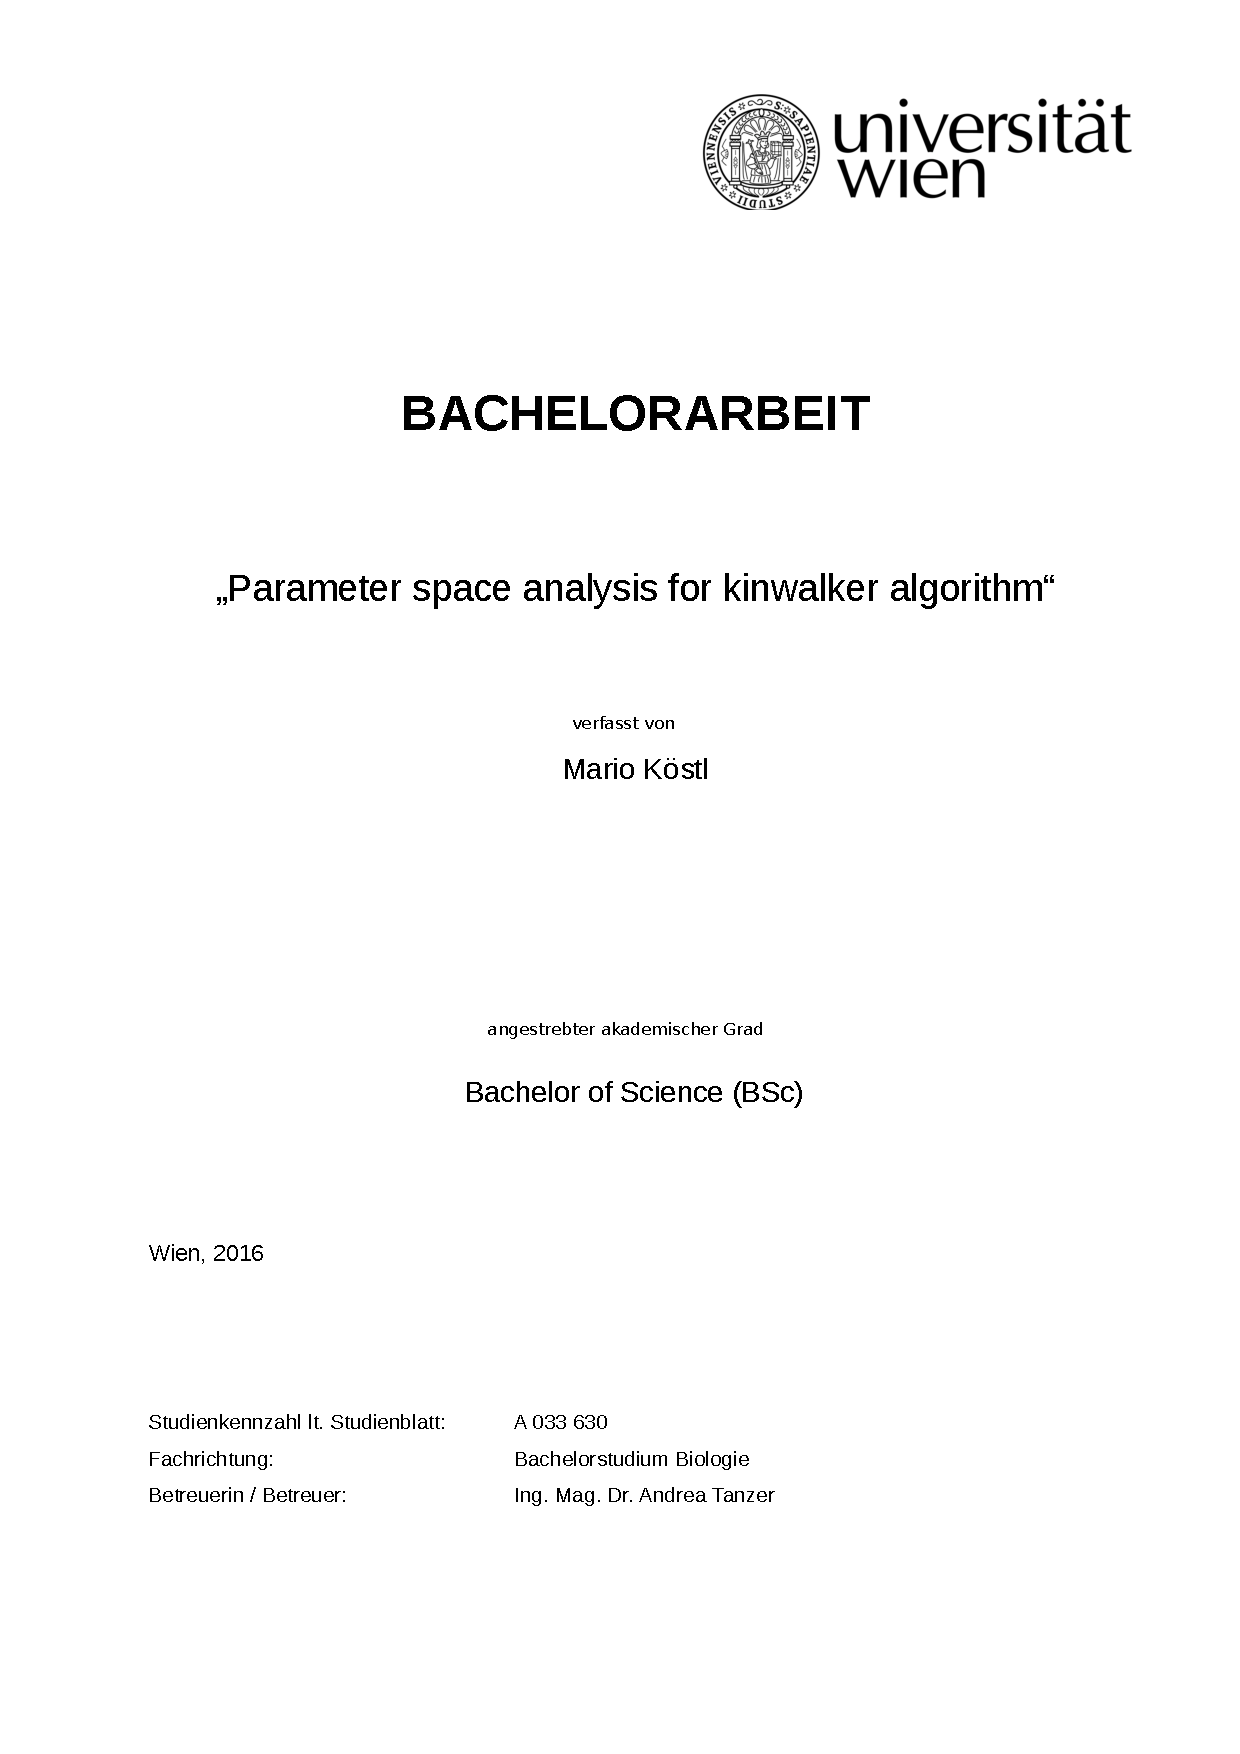
\includepdf[pages=-,pagecommand={},noautoscale=true,offset=0.5cm 0.0cm, scale=1.00, frame=false]{Deckblatt_marioBac.pdf}
\cleardoublepage
\selectlanguage{american} % american ngerman
\pagenumbering{roman}
\pagestyle{plain}
%********************************************************************
% Frontmatter
%*******************************************************
%%*******************************************************
% Little Dirty Titlepage
%*******************************************************
\thispagestyle{empty}
%\pdfbookmark[1]{Titel}{title}
%*******************************************************
\begin{center}
    \spacedlowsmallcaps{\myName} \\ \medskip                        

    \begingroup
        \color{Maroon}\spacedallcaps{\myTitle}
    \endgroup
\end{center}        

\cleardoublepage%*******************************************************
% Abstract
%*******************************************************
%\renewcommand{\abstractname}{Abstract}
\pdfbookmark[1]{Abstract}{Abstract}
\begingroup
\let\clearpage\relax
\let\cleardoublepage\relax
\let\cleardoublepage\relax

\chapter*{Abstract}
Functional RNA secondary structures are evolutionary conserved and can be predicted with various algorithms. Furthermore, RNA is able to fold onto itself during transcription, called the co-transcriptional folding event. The program kinwalker is able to predict such co-transcriptional foldings, by using a deterministic algorithm. The Kinwalker algorithm comes with different parameters, to fine tune said predictions. I performed a detailed parameter space analysis for three well studied RNA families. With the created data, evidence of evolutionary conservation of folding pathways can be investigated.




\vfill
%\selectlanguage{ngerman}
\pdfbookmark[1]{Zusammenfassung}{Zusammenfassung}
\chapter*{Zusammenfassung}



Funktionelle RNA sekund{\"a}r Strukturen sind evolution{\"a}r konserviert, und k{\"o}nnen durch verschiedene Algorithmen vorherbestimmt werden. Dar{\"u}ber hinaus kann RNA w{\"a}hrend der Transkription auf sich selbst zur{\"u}ckfalten. Dieses Ph{\"a}nomen wird auch als Co-transkriptionelles Falten bezeichnet. Das Programm Kinwalker ist in der Lage solch Co-transkriptionelles Falten vorherzubestimmen. Kinwalker hat mehrere Parameter um Feinabstimmungen am Algorithmus zu t{\"a}tigen. Ich habe eine detailierte Parameter Raum Analyse f{\"u}r drei wissenschaftlich bekannter RNA Familien get{\"a}tigt. Mit diesen erzeugten Daten, k{\"o}nnen Hinweise auf evolution{\"a}re Konservierung des Co-transkriptionellen Faltungsvorgang untersucht werden.




\endgroup			

\vfill
\cleardoublepage%*******************************************************
% Acknowledgments
%*******************************************************
\pdfbookmark[1]{Acknowledgments}{acknowledgments}


%\bigskip

\begingroup
\let\clearpage\relax
\let\cleardoublepage\relax
\let\cleardoublepage\relax
\chapter*{Acknowledgments}
Sincere thanks to everybody who helped me to succeed in writing this thesis.


%First and foremost I want to thank my supervisor Ivo L. Hofacker, who was always
%patient and helpful and guided me through the many years of my PhD study.
%His scientific competence, and that of his group, allowed me to thoroughly
%investigate new fields of research.


Very special thanks goes to Andrea and Ronny, who always helped me with every problem I came up with. Without Andrea's knowledge of biological systems and their behavior and Ronny's knowledge about coding and math, this thesis wouldn't be as detailed and informative.




Furthermore, I want to thank all my colleagues at the TBI, especially those who provided me with beer, schnapps and bacon in Bled.



\endgroup




\pagestyle{scrheadings}
\cleardoublepage%*******************************************************
% Table of Contents
%*******************************************************
%\phantomsection
\refstepcounter{dummy}
\pdfbookmark[1]{\contentsname}{tableofcontents}
\setcounter{tocdepth}{2} % <-- 2 includes up to subsections in the ToC
\setcounter{secnumdepth}{3} % <-- 3 numbers up to subsubsections
\manualmark
\markboth{\spacedlowsmallcaps{\contentsname}}{\spacedlowsmallcaps{\contentsname}}
\tableofcontents 
\automark[section]{chapter}
\renewcommand{\chaptermark}[1]{\markboth{\spacedlowsmallcaps{#1}}{\spacedlowsmallcaps{#1}}}
\renewcommand{\sectionmark}[1]{\markright{\thesection\enspace\spacedlowsmallcaps{#1}}}
%*******************************************************
% List of Figures and of the Tables
%*******************************************************
%\clearpage

%\begingroup 
%    \let\clearpage\relax
%    \let\cleardoublepage\relax
%    \let\cleardoublepage\relax
%    %*******************************************************
%    % List of Figures
%    %*******************************************************    
%    %\phantomsection 
%    \refstepcounter{dummy}
%    %\addcontentsline{toc}{chapter}{\listfigurename}
%    \pdfbookmark[1]{\listfigurename}{lof}
%    \listoffigures
%
%    \vspace*{8ex}
%
%    %*******************************************************
%    % List of Tables
%    %*******************************************************
%    %\phantomsection 
%    \refstepcounter{dummy}
%    %\addcontentsline{toc}{chapter}{\listtablename}
%    \pdfbookmark[1]{\listtablename}{lot}
%    \listoftables
%        
%    \vspace*{8ex}
%%   \newpage
%    
%    %*******************************************************
%    % List of Listings
%    %*******************************************************      
%	  %\phantomsection 
%    \refstepcounter{dummy}
%    %\addcontentsline{toc}{chapter}{\lstlistlistingname}
%    \pdfbookmark[1]{\lstlistlistingname}{lol}
%    \lstlistoflistings 
%
%    \vspace*{8ex}
%       
%    %*******************************************************
%    % Acronyms
%    %*******************************************************
%    %\phantomsection 
%    \refstepcounter{dummy}
%    \pdfbookmark[1]{Acronyms}{acronyms}
%    \markboth{\spacedlowsmallcaps{Acronyms}}{\spacedlowsmallcaps{Acronyms}}
%    \chapter*{Acronyms}
%    \begin{acronym}[UML]
%        \acro{DRY}{Don't Repeat Yourself}
%        \acro{API}{Application Programming Interface}
%        \acro{UML}{Unified Modeling Language}
%    \end{acronym}                     
%\endgroup

\cleardoublepage
%********************************************************************
% Mainmatter
%*******************************************************
\pagenumbering{arabic}
\cleardoublepage

\chapter{Introduction}

RNA is a polymer molecule, consisting of smaller sub-units called
nucleotides. A nucleotide is composed of a nucleobase, a ribose
monosaccharid and a phosphate group. The nucleobase can either be an
Adenin(A), Cytosin(C), Uracil(U) or a Guanin(G). Nucleotides are linked
together by covalent bonds, resulting in a sugar-phosphate backbone. In
contrast to RNA, DNA replaces the nucleobase U with a Thymin(T), and the
ribose with a deoxyribose, which lacks a hydroxyl group on the C2 of
the ribose sugar.  Both DNA and RNA are directional molecules with a 5 prime end (5';
the C5 of the ribose) and a 3 prime end (3'; the C3 of the ribose). The
sequence of a gene is read from 5' to 3'.

RNAs are essential for every living organism and play a major role in
regulation of various cellular processes such as
transcription, splicing, translation and RNA degradation
\citep{Mattick15042006}.

RNAs are formed during transcription, executed by different RNA polymerases. In detail, the DNA template strand (3'-> 5') is read by a RNA polymerase and a new single RNA strand is formed, with complementary bases. The newly formed strand (5'-> 3') is now an exact copy of the DNA leading strand (5' -> 3'). The RNA polymerase is a nucleotidyl transferase which catalysis the polymerization of ribonucleotides on the 3' end of a new RNA strand.

%%basepair definition -----------------------

RNA sequences can be abstracted to 4 different structure levels, called the
primary, secondary, tertiary and quaternary structure. Within this thesis,
only primary and secondary structures are addressed. The primary structure
is the sequence of ribonucleotids from the 5' to the 3' end. Secondary
structures are defined by base-pairs, which are formed by hydrogen bonds between nucleobases 
leading to a 2 dimensional structure. Regarding RNA, hydrogen bonds can
occur between G-C and  A-U (Watson Crick pairs) and G-U (Wobble Pairs ), whereby the G-C base pair is more stable, due to three hydrogen bonds instead of the two bonds of the G-U or A-U base-pair.

RNA tertiary structures represent all further bonds, that will lead to its spatial conformation, and quaternary structures would be interactions of such tertiary structures with themselves. Such quaternary structures can be found in the ribosome or the spliceosome\citep{spliceosome}.
From now on, only secondary structures are considered within my thesis.

\begin{figure}
  \begin{center}
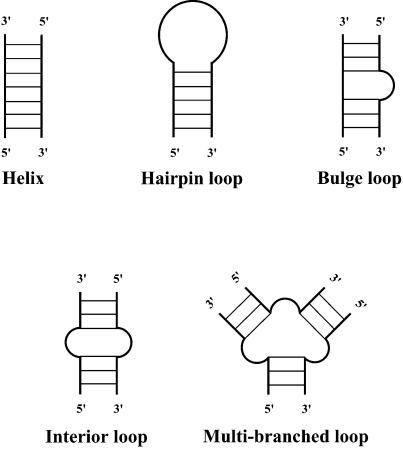
\includegraphics[width=0.5\textwidth]{./pictures/secondary_structure_motifs.jpg}
  \end{center}
\caption{{\bf frequently appearing RNA secondary structure motifs\citep{SecondaryStructureMotifs}.}  
RNA secondary structures are defined by base-pairs, which are formed by hydrogen bonds between nucleobases 
leading to a 2 dimensional structure.}
\label{fig:secondaryStructureMotifs}
\end{figure}

\FloatBarrier
From a mathematical point of view, secondary structures can be represented as lists of base-pairs (i, j), with
i\textless j, where i is a base that can form a base-pair with base j and $i\not=j$\citep{waterman1978}.
\begin{enumerate}
	\item each nucleotide (nt) i takes part in at most one base pair (base triplets are not allowed)
	\item $j- i$ \textgreater 3 (the most simple hairpin loop consists of minimal 3 non paired bases)
	\item two base-pairs (i, j) and (k, l) do not cross, if i\textless k\textless j then k\textless l\textless j (pseudoknots are not allowed)
\end{enumerate}
This notation will be used throughout my thesis.


%%MFE description-----
%Secondary structure formation is depending on the primary sequence of the RNA as well as the free energy of the formed structure. 



An RNA sequence can fold into a variety of structures with different free
energies, stability and probability to be observed.
The more stable a structure, the more frequently it is found within the
Bolzmann distributed ensemble of structures. The most frequent structure is
the one with the lowest free energy, the so called minimal free energy
structure (MFE).
The active structure in nature (i.e. the native structure) could differ to their MFE structure, because the
native structure doesn't have to be the energetically lowest one.

%The free energy defines the stability of such structures and if this structure is able to form after all. If the free energy is lower, the structure is more stable and the possibility of formation is increased. The structure of a sequence with the lowest free energy is called the minimal free energy structure (MFE). The native structure could differ to their MFE structure, because the active structure doesn't have to be the energetically lowest one.

Many efficient algorithms are available to predict secondary structures
from RNA sequences \citep{hofacker:1994},\citep{ViennaRNA},\citep{Mfold},\citep{Contrafold}. The basic idea here is to 
decompose secondary structures into their building blocks, i.e. loops like
hairpins, bulges, interior loops or multi loops (fig.~\ref{fig:secondaryStructureMotifs}).
In turn, the free energy of an RNA secondary structure can be calculated by
summing up the energies of the individual loops it consists of.

The tools of the \texttt{ViennaRNA package 2.0} \cite{ViennaRNA}, like
\texttt{RNAfold}\cite{RNAfoldWebsite} predict secondary structures using a
physics based model. In this model, the energy parameters of individuel
loop types were determined by RNA melting experiments of hundreds of
different RNA sequences \cite{turner:1987},\cite{mathews:99},\cite{mathews:2002},\cite{turner:2009}.  The recursively
dynamic programming algorithm introduced by \citet{zuker:1981} allows for
fast and efficient prediction of secondary structures.


Throughout this thesis only {\it in vitro} folding is considered, therefore
we neglect any \emph{in vivo} environmental factors, such as RNA
chaperones, RNA binding proteins (RBPs), small ligands or
ion-concentration.

\section{Co-transcriptional RNA folding prediction}

RNAs are in constant flux between different structural conformations.
This is of particular interrest during transcription, because with every
nucleotide added the set of possible conformations increases
exponentially. Like all molecules, RNAs are driven towards their most stable
conformation, i.e. the MFE structure. 
In nature, the MFE structure is not necessarily the predominant one. During
the folding process the RNA might get caught in another stable low energy
structure. Such folding traps and trajectories folding directly into the MFE can be predicted using kinetic folding
algorithms discussed in this section.

%The structural ensemble of an RNA sequence is determined by it's Boltzmann distribution.

%as for instance bacterial riboswitches and ribozymes\citep{ribozym}. 
During transcription the new RNA strand is created starting with the 5'
end, therefore RNA folding can also occur during transcription at the
extending 3' end\cite{Kramer1981}.
Additional structures emerge at the 3' end of the newly synthesized sequence during transcription, which in turn can trigger refolding of the upstream region.



%%------------------ KINWALKER description
In contrast to MFE prediction, computing co-transcriptional folding pathways of
RNAs is extremely difficult and thus only a handful of programs exist which
allow for an efficient prediction. One of them is the program
\texttt{Kinwalker\cite{kinwalker}}. \texttt{Kinwalker} aims to substitute
the effort of predicting RNA folding kinetics by using an heuristic approach, that
deterministically follows the most favorable folding trajectory. For that
purpose, it makes use of MFE predictions for each substructure in the
sequence intervals [i,j].
Thus, secondary structure predictions for unfinished RNA chains during transcription is possible.
\texttt{Kinwalker} implements various path-finding algorithms to calculate structural changes during and after transcription. Further details of these algorithms are described in section~\ref{kinwalker parameter description}.

One of the first steps of the \texttt{Kinwalker} algorithm is to create the
$C$ matrix. This matrix consists of MFE values ranging from sequence
position $i$ to $j$. To calculate this matrix, every possible
$(x_i,...,x_j)$ sub-sequence is taken and the respective MFE structure is
calculated. The resulting sub-structure for the sub-sequence $(x_i,...,x_j)$ is called $s_{i,j}$. 
The exact same matrix is also used in the program RNAfold to
predict global MFE structures, i.e. the MFE structure for the full length
RNA.
In contrast, \texttt{Kinwalker} calculates the most likely structure for
every trajectory step, which is not necessarily the MFE structure of
the already transcribed sub-sequence.  

Every cycle of transcription adds one base to the growing 3' end,
therefore sequences with different length are present during
transcription. At the beginning of each step we have the current
structure $s_{i,j}$ and have to find a way to the structure $s_{i,j+1}$. To do so,
\texttt{Kinwalker} makes use of all the MFE sub-structures backtracked from
the $C$ matrix. Every possible sub-structure is used as a candidate that
might be merged into the structure trajectory.


\texttt{Kinwalker} decides on sub-structures depending on the path-finding
algorithm used. If a sub-structure has been selected, it will not be
considered any further and removed from matrix $C$. After each
transcription step, structures $s_{i,j}$ and $s_{i,j+1}$ are
merged. Special algorithms are implemented, to resolve base-pair conflicts
during the merge. The \texttt{Kinwalker} algorithm is able to predict
folding trajectories of RNA sequences of up to 1500 nucleotides in length. 
Different parameters can be used to execute the \texttt{Kinwalker}
algorithm.

The optimal parameter set for RNA co-transcriptional folding prediction has
never been analyzed in great detail.  Some parameters reflect reality more
than others. The best parameter combinations remain to be determined in
order to increase precision of \textit{in silico} folding prediction of RNA
structures.



\subsection{TRP operon}

The regulation of the TRP operon is a good biological example for RNA co-transcriptional folding and is therefore used within this thesis.
The TRP operon is a DNA sequence consisting of 5 genes (i.e. trpE, trpD, trpC, trpB, trpA), each of them encoding the tryptophan synthetase protein which is essential for tryptophan synthesis, and some regulatory areas, described below.
The TRP operon is found throughout the enterobacteriaceae family, but is missing in
eucaryotes and archaea. In bacteria, transcription and translation occurs
more or less simultaneously and thus regulating one may affect the
other.
Genes of operons are clustered into logical groups and are therefore transcribed and regulated together.
The regulatory region of the TRP operon, located upstream of the 5 coding genes, consists of the tryptophan repressor gene trpR (coding for the trp repressor protein), the tryptophan leader transcript (trpL), the promoter (P) and the operator (O). The promoter is the binding site for the RNA polymerase and the operator is the binding site for the trp repressor protein.

Regulation of TRP synthesis is essential for maintaining homeostasis inside the bacterial cell, to prevent intoxication from TRP over-production, as well as energy conservation if enough TRP is available.
If tryptophan is present in the cell, the genes for trypthopan synthesis
should be inactivated and vica verse. 
The TRP operon is regulated by two different systems, a repressive negative regulation via trpR (fig.~\ref{fig:trp_operon_trpR}) and a regulation via secondary structures (i.e. attenuation fig.~\ref{fig:trp_operon_attenuation}). 

Repressive negative regulation is triggered by binding of TRP molecules to the trp repressor protein, which will change its structural conformation and can now bind to the operator, stopping transcription initiation. If TRP is absent, trp repressor cannot bind to the operator and transcription of tryptohpan synthetase genes is possible, leading to newly synthesized TRP.

Attenuation is correlated with the formation of secondary structures
(i.e. two different hairpins) of trpL\cite{Oxender1979},
\cite{Yanofsky1977}. In difference to the trpR system which targets
intracellular TRP and regulates transcription initiating, attenuation
targets TRP already loaded onto tRNAs and regulates gene expression during transcription.

\texttt{TrpL} consists of 4 sequence areas (seq 1, seq 2, seq 3, seq 4) which are in
part complementary to each other and therefore able to form 3 different hairpins: 1-2, 2-3, 3-4.
Seq 1 codes for multiple tryptophans, seq 2 can form a rather unstable hairpin with seq 1, or a stable hairpin with seq 3 (i.e. the anti terminator hairpin), and seq 3 can form another stable hairpin with seq 4 (i.e. the terminator hairpin).
A formation of the terminator hairpin leads to transcription stop, whereby the formation of the antiterminator hairpin will not stop transcription. 

Forming of the antiterminator hairpin, and therefore preventing the
terminator hairpin, requires some time and is therefore only possible if
the ribosome is stalled upstream seq 2. The key to ribosome stalling is
hidden in seq 1 which contains multiple consecutive TRP-codons. Low level
of intracellular TRP and therefore a low level of TRP loaded tRNAs stall
the ribosome at seq 1, which will lead to the formation of the
antiterminator hairpin and correct transcription of the structural genes. 
High level of intra-cellular trypthophan and therefore a high level of TRP
loaded tRNAs lead to faster translation of seq 1 and thus covering of seq 2 by the ribosome. Therefore the formation of the terminator hairpin and the dissociation of the polymerase is possible, which will lead to transcription stop. 

\begin{figure}
  \begin{center}
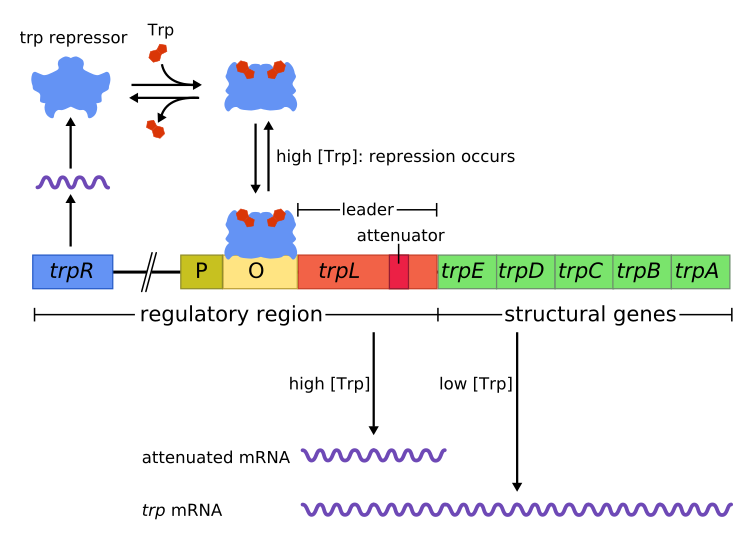
\includegraphics[width=0.7\textwidth]{./pictures/Discussion_results/TRP/Trpoperon_trpR.png}
  \end{center}
\caption{{\bf TRP operon repressive negative regulation via trpR.} Repressive negative regulation occurs if enough TRP molecules have bound to the trp repressor protein, which will change its structural conformation and can now bind to the operator sequence, leading to transcription stop. If TRP is absent, trp repressor cannot bind to the operator(O) and transcription of tryptohpan synthetase genes is possible, leading to new TRP.}
\label{fig:trp_operon_trpR}
\end{figure}

\begin{figure}
  \begin{center}
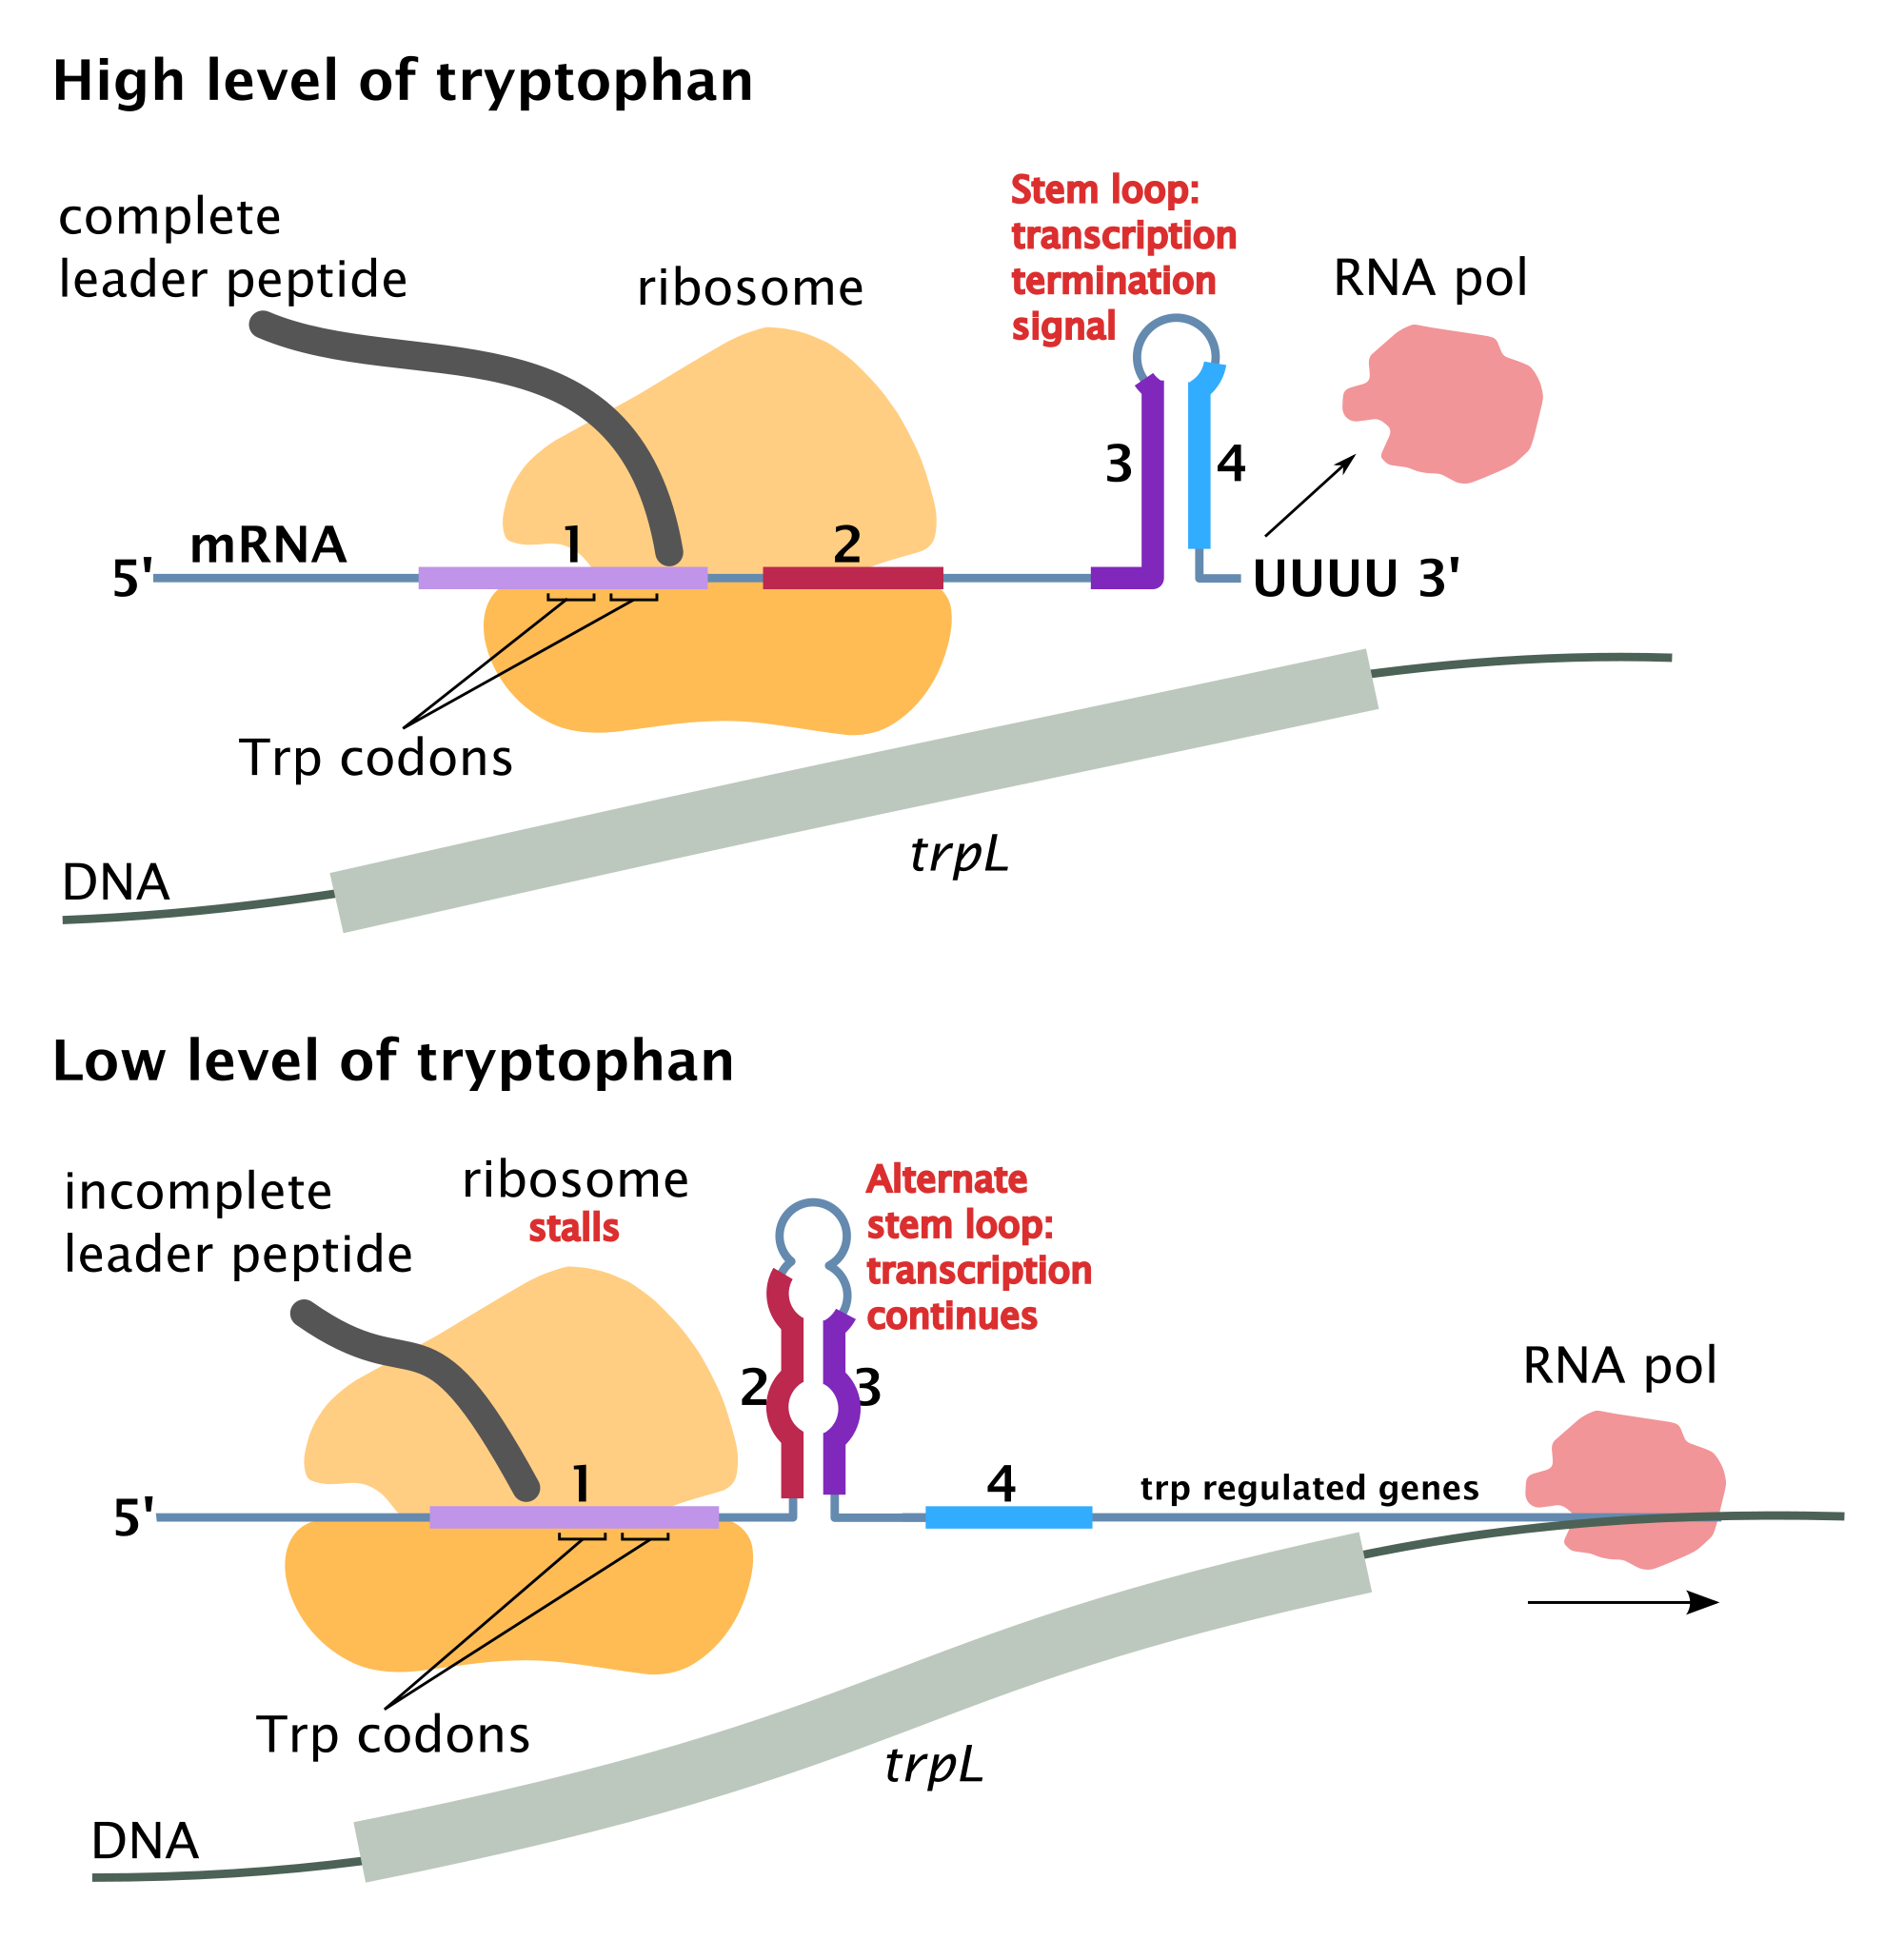
\includegraphics[width=0.7\textwidth]{./pictures/Discussion_results/TRP/trp_operon_attenuation.png}
  \end{center}
\caption{{\bf Regulation of TRP operon via secondary structures (attenuation).} 
upper panel: High level of intra-cellular trypthophan and therefore a high level of TRP loaded tRNAs leads to faster translation of seq 1 and covering of seq 2 by the ribosome. Therefore the formation of the terminator hairpin and the dissociation of the polymerase, is possible, which will lead to transcription stop. 
  lower panel: Low level of intracellular TRP and therefore a low level of TRP loaded tRNAs stalls the ribosome at seq 1, which will lead to the formation of the antiterminator hairpin and correct transcription. }
\label{fig:trp_operon_attenuation}
\end{figure}


\FloatBarrier

\section{Motivation}

%It is interesting and worth knowing, how different RNA sequences behave during co-transcriptional folding, if evolutionary conserved folding pathways are present, and if they can be predicted by the \texttt{Kinwalker} algorithm.
%To examine how fine tuning of the \texttt{Kinwalker} parameter influence predictions, a detailed parameter space analysis was performed. Due to comparisons with experimentally evaluated structures, the validity of the performed structure predictions can be analyzed. 
%To understand the evolutionary conservation of related RNA sequences, and their folding pathways, co-transcriptional folding analysis is necessary,

It is from uttermost importance to analyze co-transcriptional folding pathways to understand evolutionary conservation of related RNA sequences and their folding pathways. These data can be used to support predicting of phylogenetic relationships, and the evolutionary history (i.e. duplication, mutation, specification,..) of RNA sequences. This thesis focuses mainly on the following questions:

\begin{itemize}
\item Are evolutionary conserved folding pathways present in related RNA sequences?
\item Is it possible to predict such pathways by using heuristics like \texttt{Kinwalker}?
\item How should the \texttt{Kinwalker} parameters be fine-tuned to better reflect reality?
\end{itemize}



\section{Outline}
I approached this questions by using \texttt{in-silico} predictions, and therefore I performed a detailed parameter space test for the program \texttt{Kinwalker}.
A total of 200 different \texttt{Kinwalker} parameter combinations were
tested on well studied RNA families.
The resulting structure trajectories were compared between different RNA
sequences of one family to determine similarities in their
co-transcriptional folding pathways. Furthermore, resulting trajectories
were compared to existing reference structures in order to determine the
optimal \texttt{Kinwalker} parameters.
\texttt{Kinwalker} trajectories were statistically analyzed with the use of python scripts and plotted for better comparison. 

%The signal recognition particle (\texttt{SRP}), tryptophan leader transcript (trpL) and the bacterial ribonuclease P (RNAseP) fit perfectly. These RNA classes are good examples for RNAs with co-transcriptional folding and therefore ideal for testing of conserved folding evolution within each family. Detailed description of these classes is found in section ~\ref{data description}. By statistical evaluation of the output data, similar and/or different behavior of sequences, during co transcriptional folding, can be obtained. 




\chapter{Materials and Methods}

\section{data description} \label{data description}

\subsection{Input files and input data}


The signal recognition particle (\texttt{SRP})\cite{SRP}, tryptophan leader
transcript (trpL)\cite{sourceRefTRP} and the bacterial ribonuclease P
(RNaseP)\cite{RNAseP} are used in this thesis, because they are well studied RNA classes with existing benchmark studies. Furthermore, for this families, reference structures and partial co-transcriptional folding intermediates are availabe.

\texttt{SRP} is a ribonucleoprotein consisting of both RNA and protein
components. \texttt{SRP} facilitates peptid transfer into the eukaryotic ER membran
or to the prokaryotic plasma membran and is therefore used as a molecular
adapter. For my analysis here only the RNA part of \texttt{SRP} is used.

  
\texttt{TrpL} is a regulatory region of the bacterial tryptophan operon and resides
upstream of the structural genes.
\texttt{TrpL} regulates gen expression via formation of two secondary RNA structures (i.e. terminator and antiterminator hairpin). Both hairpins can be formed during transcription and are good examples for co-transcriptional folding of RNA. 


\texttt{RNaseP} is a ribozym - a ribonucleic acid that is able to catalyze chemical
reactions - is found throughout all domains of life (bacteria, archaea and
eukaryotes). \texttt{RNaseP} catalyzes the cleaving of the 5' leader sequence of precursors tRNA and is also important in correct transcription of various small noncoding RNAs (i.e. 5s rRNA, \texttt{SRP} RNA). 



The original alignment data for each RNA class were obtained from the
Rfam\cite{Rfam} database version 12.0 and further processed\cite{Meyer}. Our working
group modified the Rfam alignments and we are currently using them as
benchmarking sets. 
%Table \ref{table:alignment composition} lists all sequences for each RNA family used in this study, 
Table:\ref{table:alignment description} provides further information on
reference sequences, their reference structures and respective
citations. Table:\ref{table:reference structures} shows the secondary structure representation of the reference structures. Reference sequences were downloaded from \texttt{NCBI database} in \texttt{FASTA} format. 
\texttt{FASTA} format is a simple plain text format used for DNA, RNA and
Aminoacid sequences. A fasta file consists of one or more entries where
each entry consist of at least two lines, a header (">" character and the sequence
identifier), folowed by subsequent lines that contain the sequence itself.

\begin{table}[ht]
\begin{tabular}{l|l|l|l|l}  
{RFam family} & {RNA class} & {ref. seq.} & {ref. struct.} & citation\\  
\hline
RF00169 & \texttt{SRP} & X01074.1/ & functional & \cite{sourceRefSRP1}, \cite{sourceRefSRP2}\\ 
 & & 170-275 & transient & \\ 
 \hline
RF00513 & \texttt{trpL} & AE005174.2/ & antiterminator& \cite{sourceRefTRP} \\
 & & 2263095-2263188 & terminator &  \\
 \hline
RF00010 & \texttt{RNaseP} & CP001509.3/ & functional & \cite{sourceRefRNAseP1}, \cite{sourceRefRNAseP2}\\
 & & 3136785-3136410 & & \\
 \end{tabular} 
\caption{{\bf alignments and corresponding reference sequences and reference structures.} \texttt{SRP} = signal recognition particle. \texttt{TrpL} = tryptophan leader transcript. \texttt{RNaseP} = bacterial ribonuclease P. }
\label{table:alignment description}
\end{table}



\begin{table}
%\begin{tabular}{p{8cm}|p{8cm}}
\begin{tabular}{l|l}
  \hline
  \multicolumn{2}{l}{{\bf \texttt{SRP}}}\\
  \hline
X01074.1 functional structure & X01074.1 transient structure \\
\hline \\[5pt]
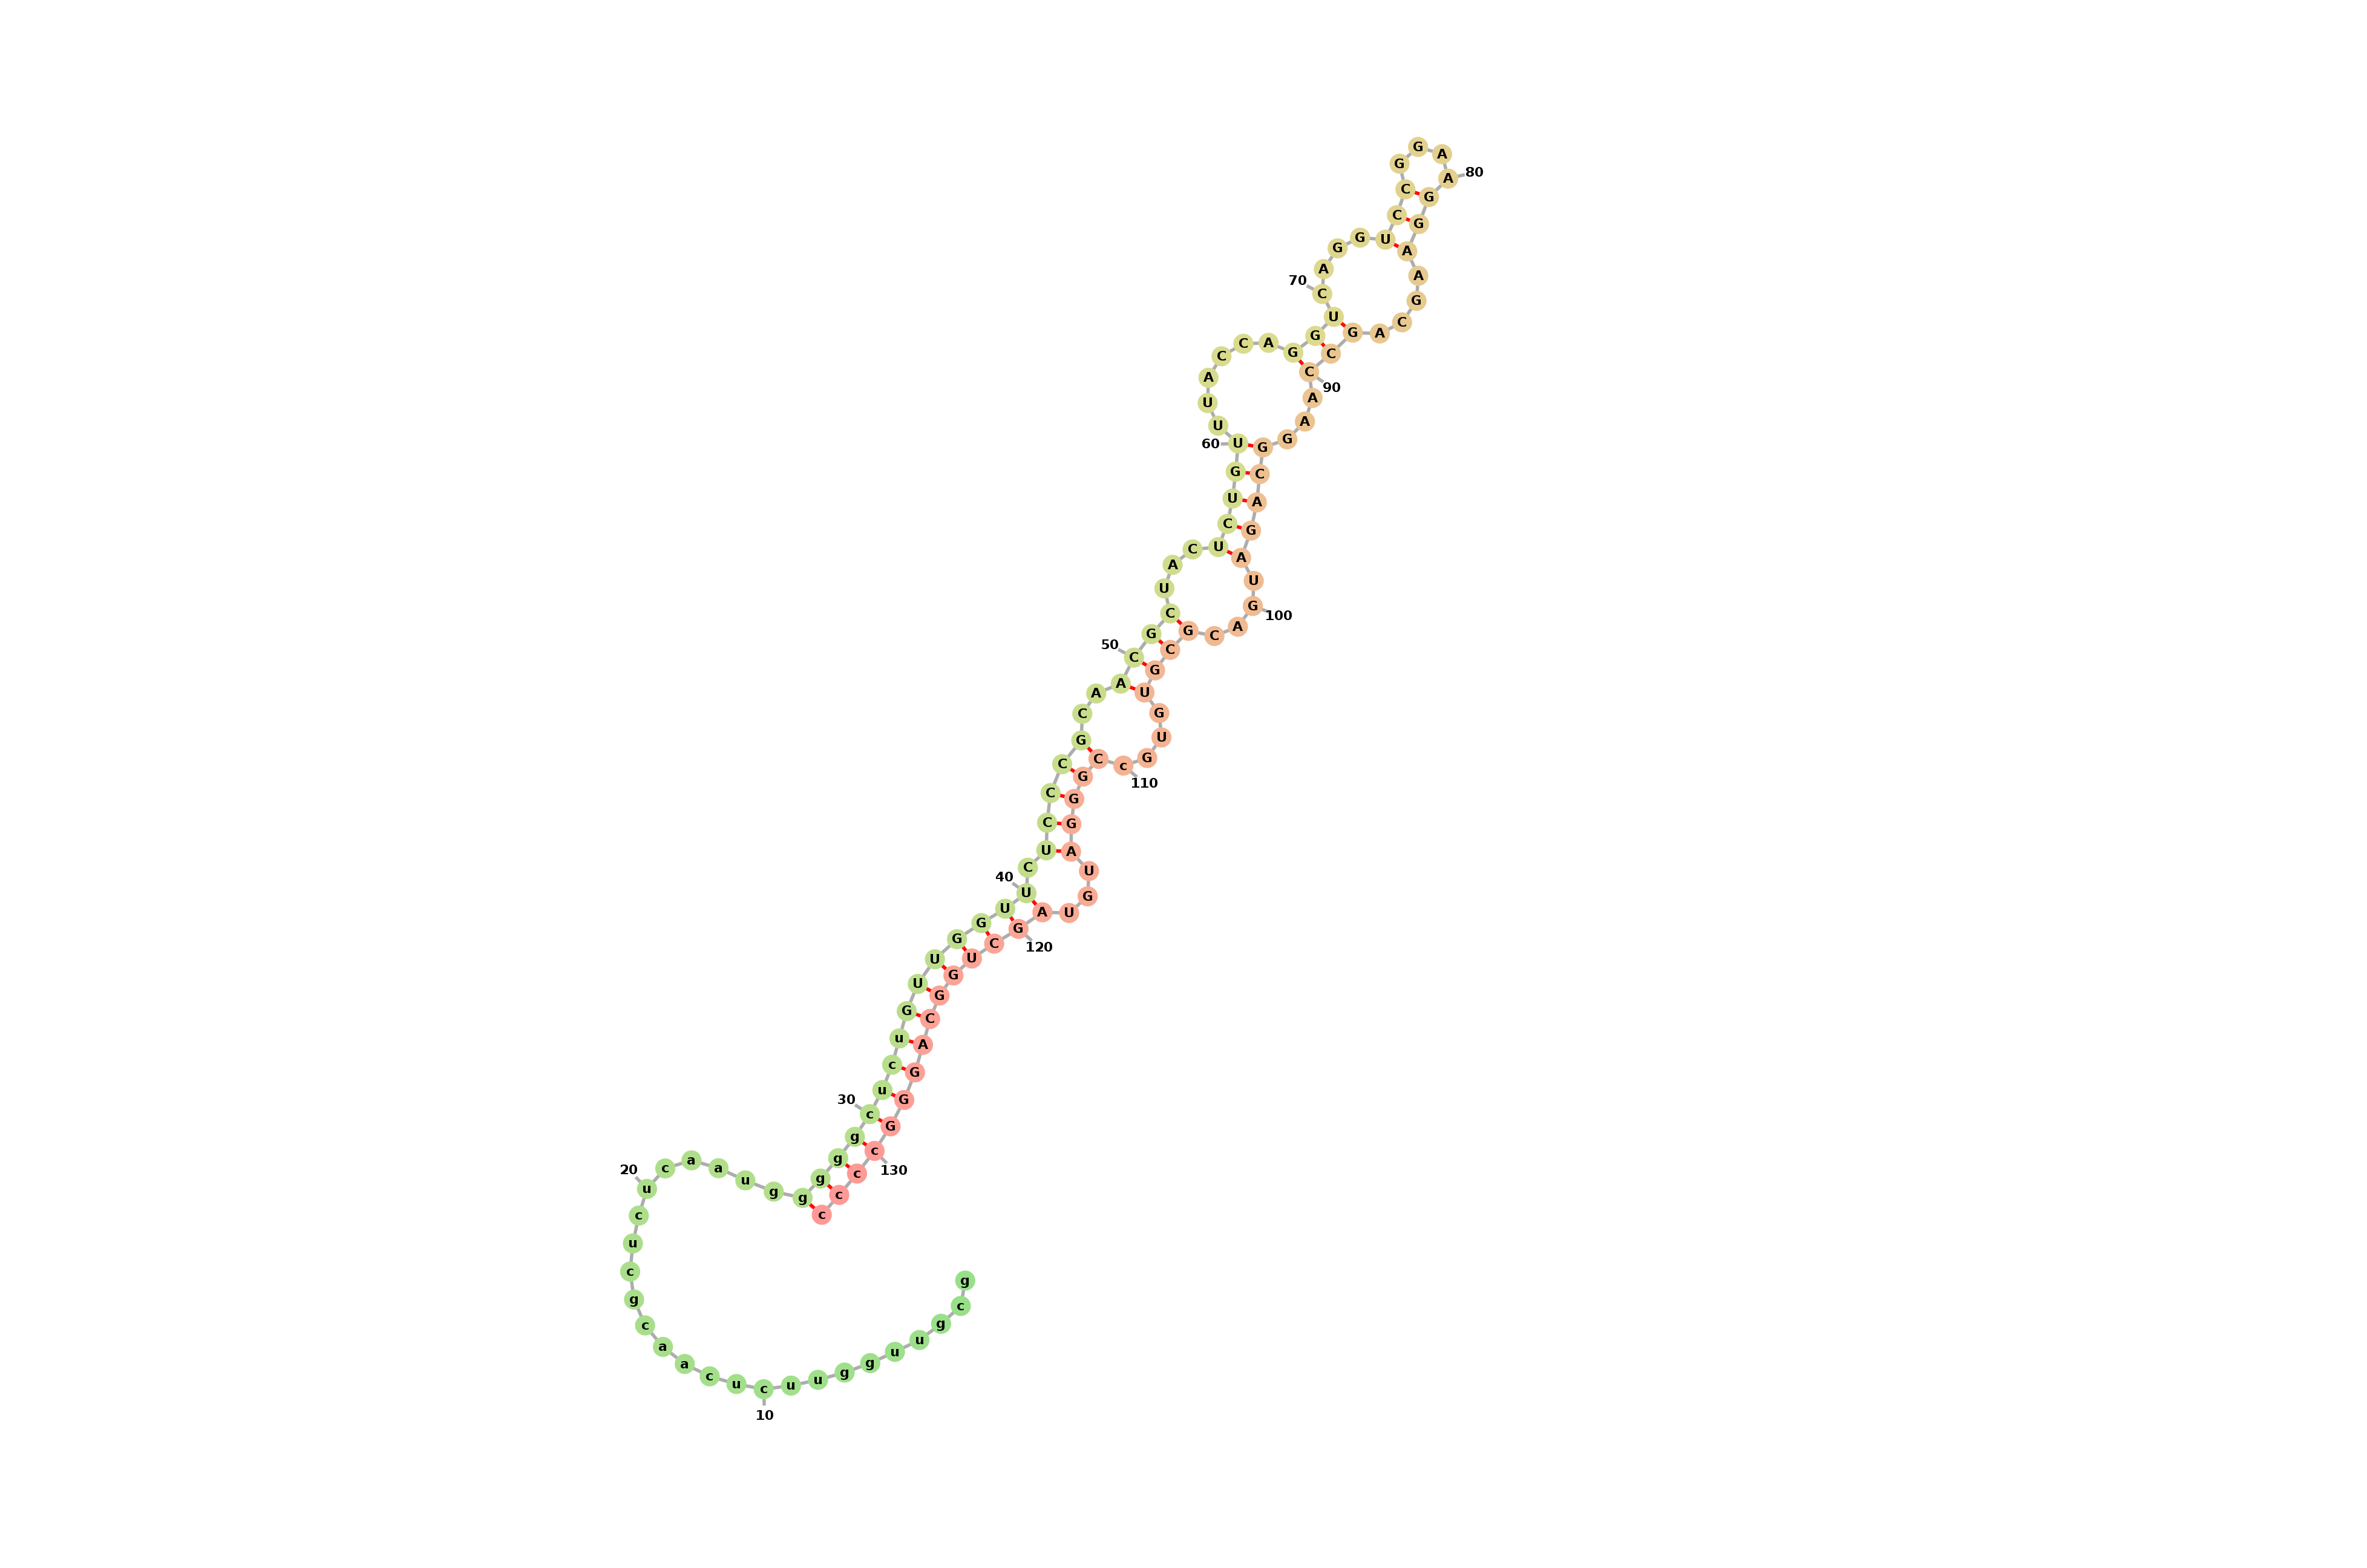
\includegraphics[width=0.5\textwidth]{./pictures/refStructure_pictures/X01074-1-functional-str.png} &
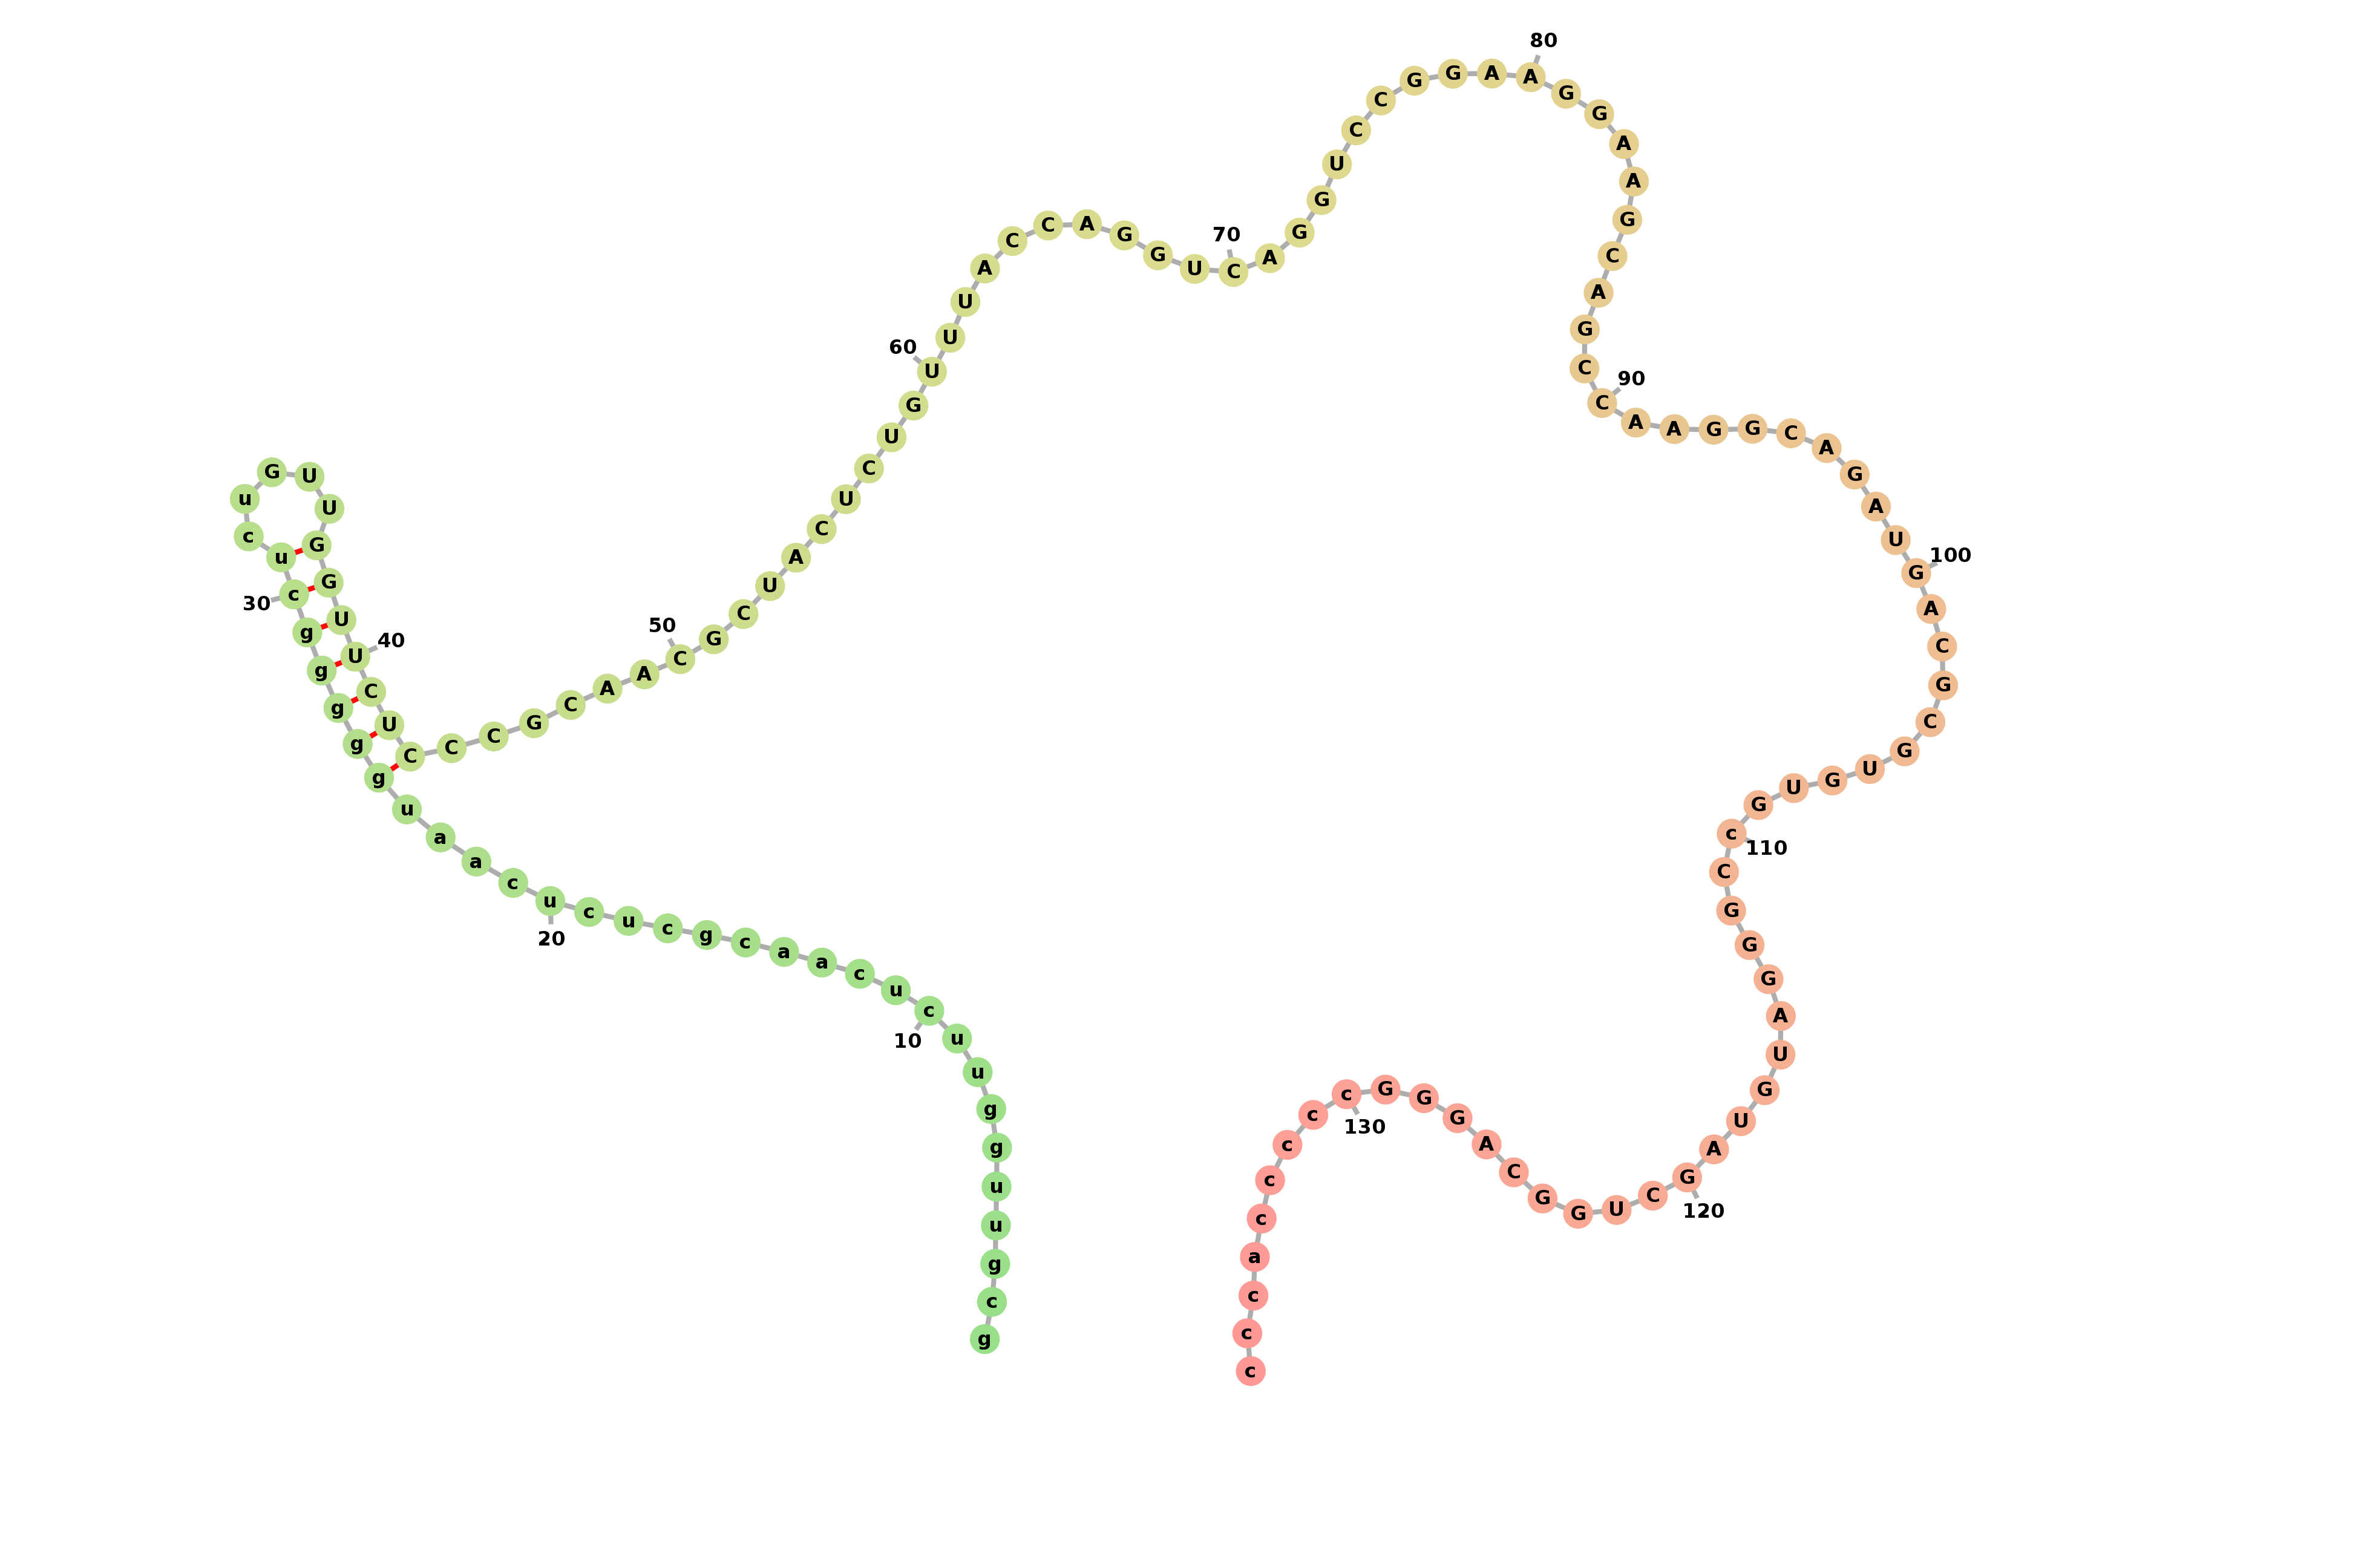
\includegraphics[width=0.5\textwidth]{./pictures/refStructure_pictures/X01074-1-transient-str.png} \\
\hline
  \multicolumn{2}{l}{{\bf trpl}}\\
  \hline
AE005174.2 antiterminator & AE005174.2 terminator\\
\hline \\[5pt]
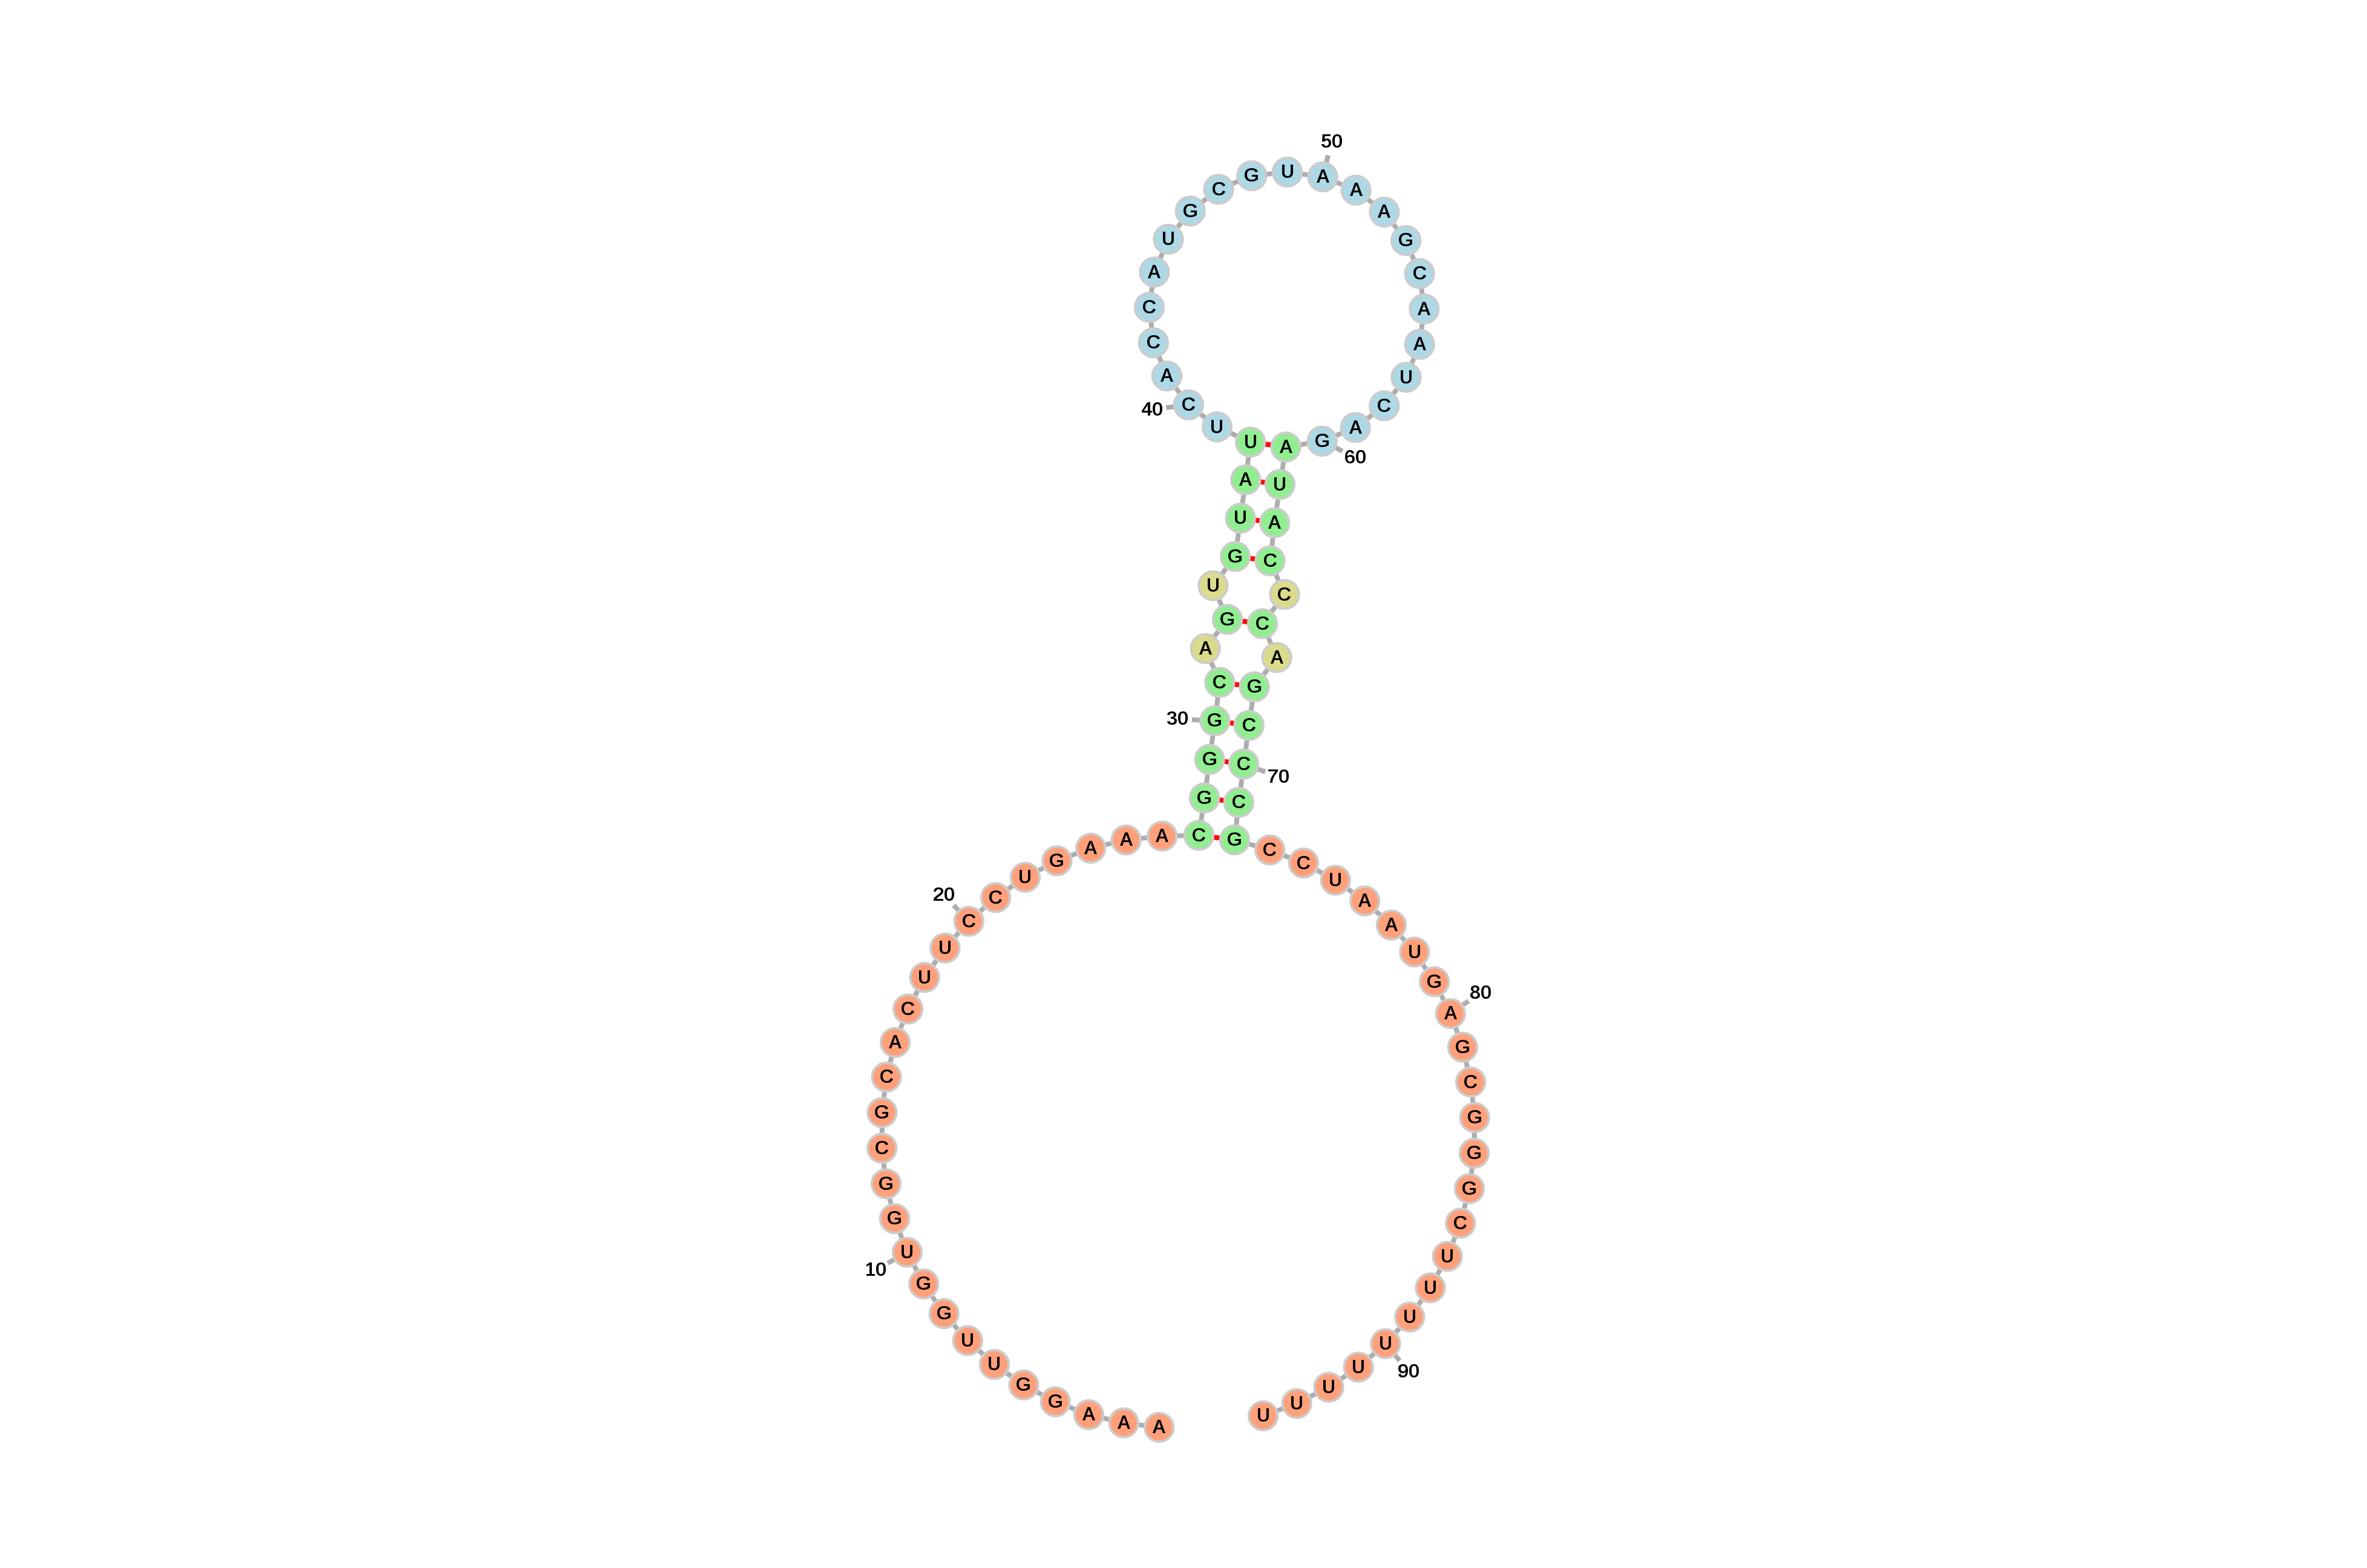
\includegraphics[width=0.5\textwidth]{./pictures/refStructure_pictures/AE005174-2-alternative1-str.png} &
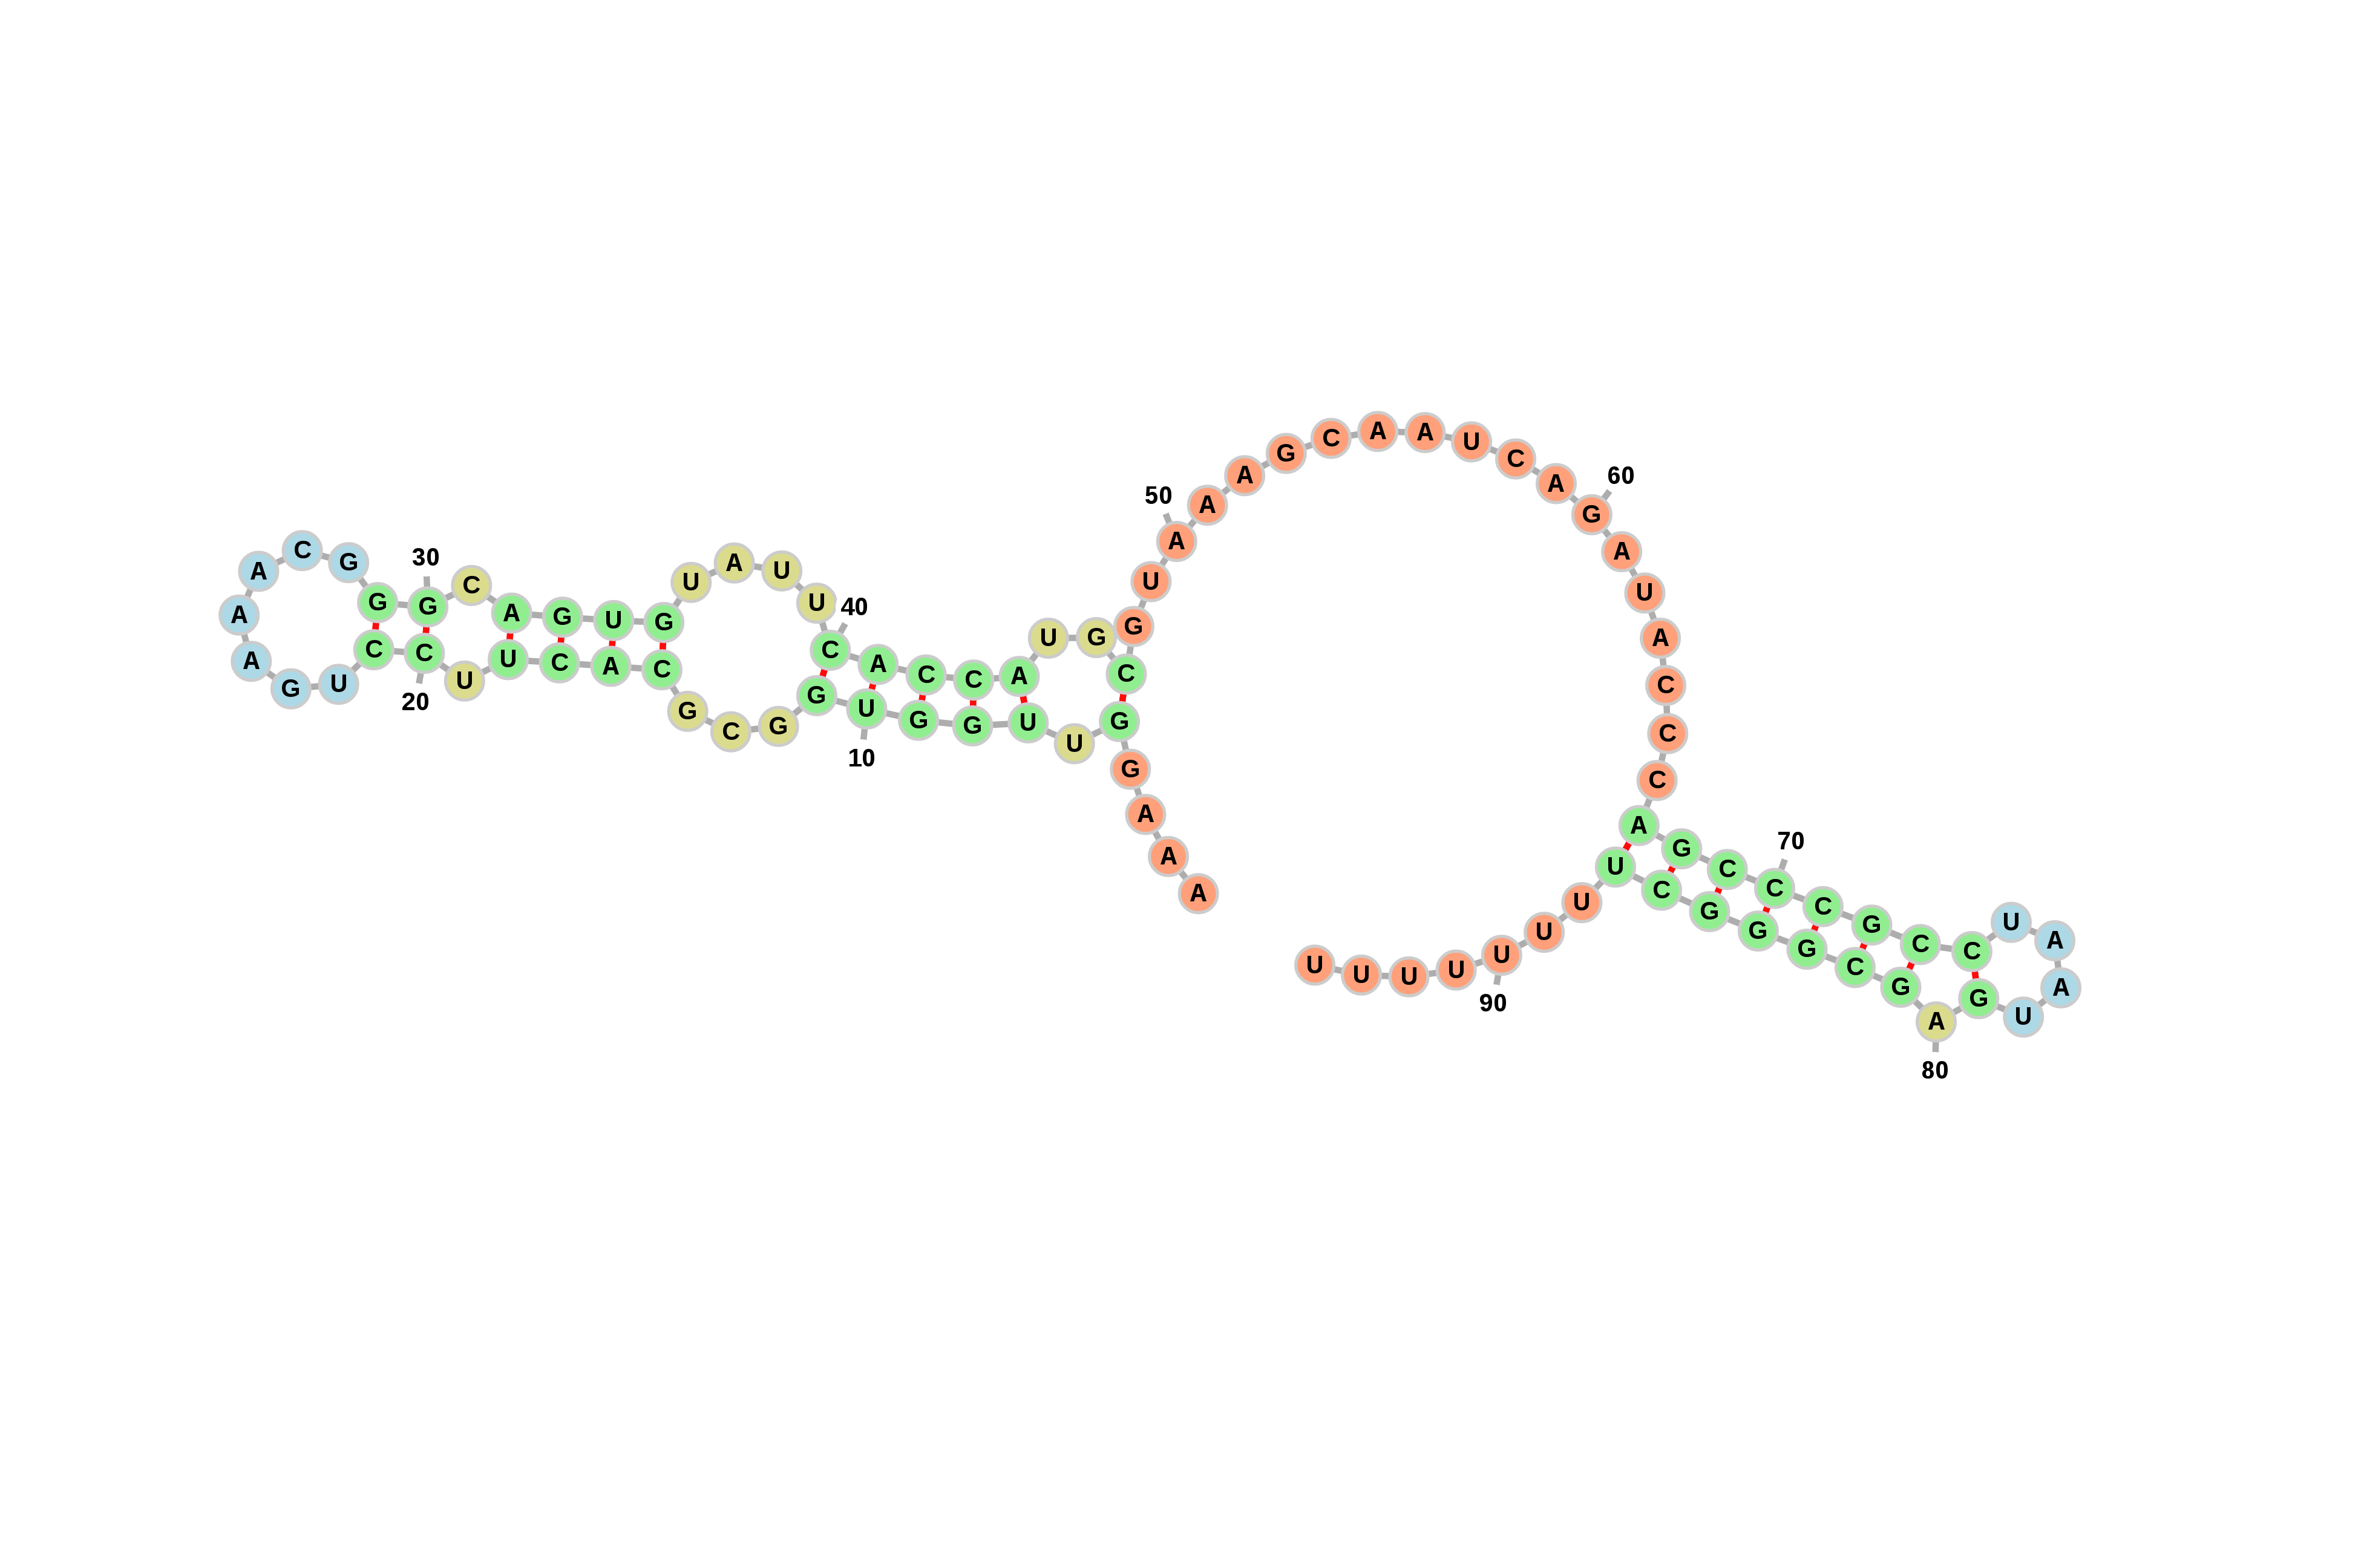
\includegraphics[width=0.5\textwidth]{./pictures/refStructure_pictures/AE005174-2-alternative2-str.png} \\
\hline
  \multicolumn{2}{l}{{\bf RNaseP}}\\
  \hline
CP001509.3 functional & \\
\hline \\[5pt]
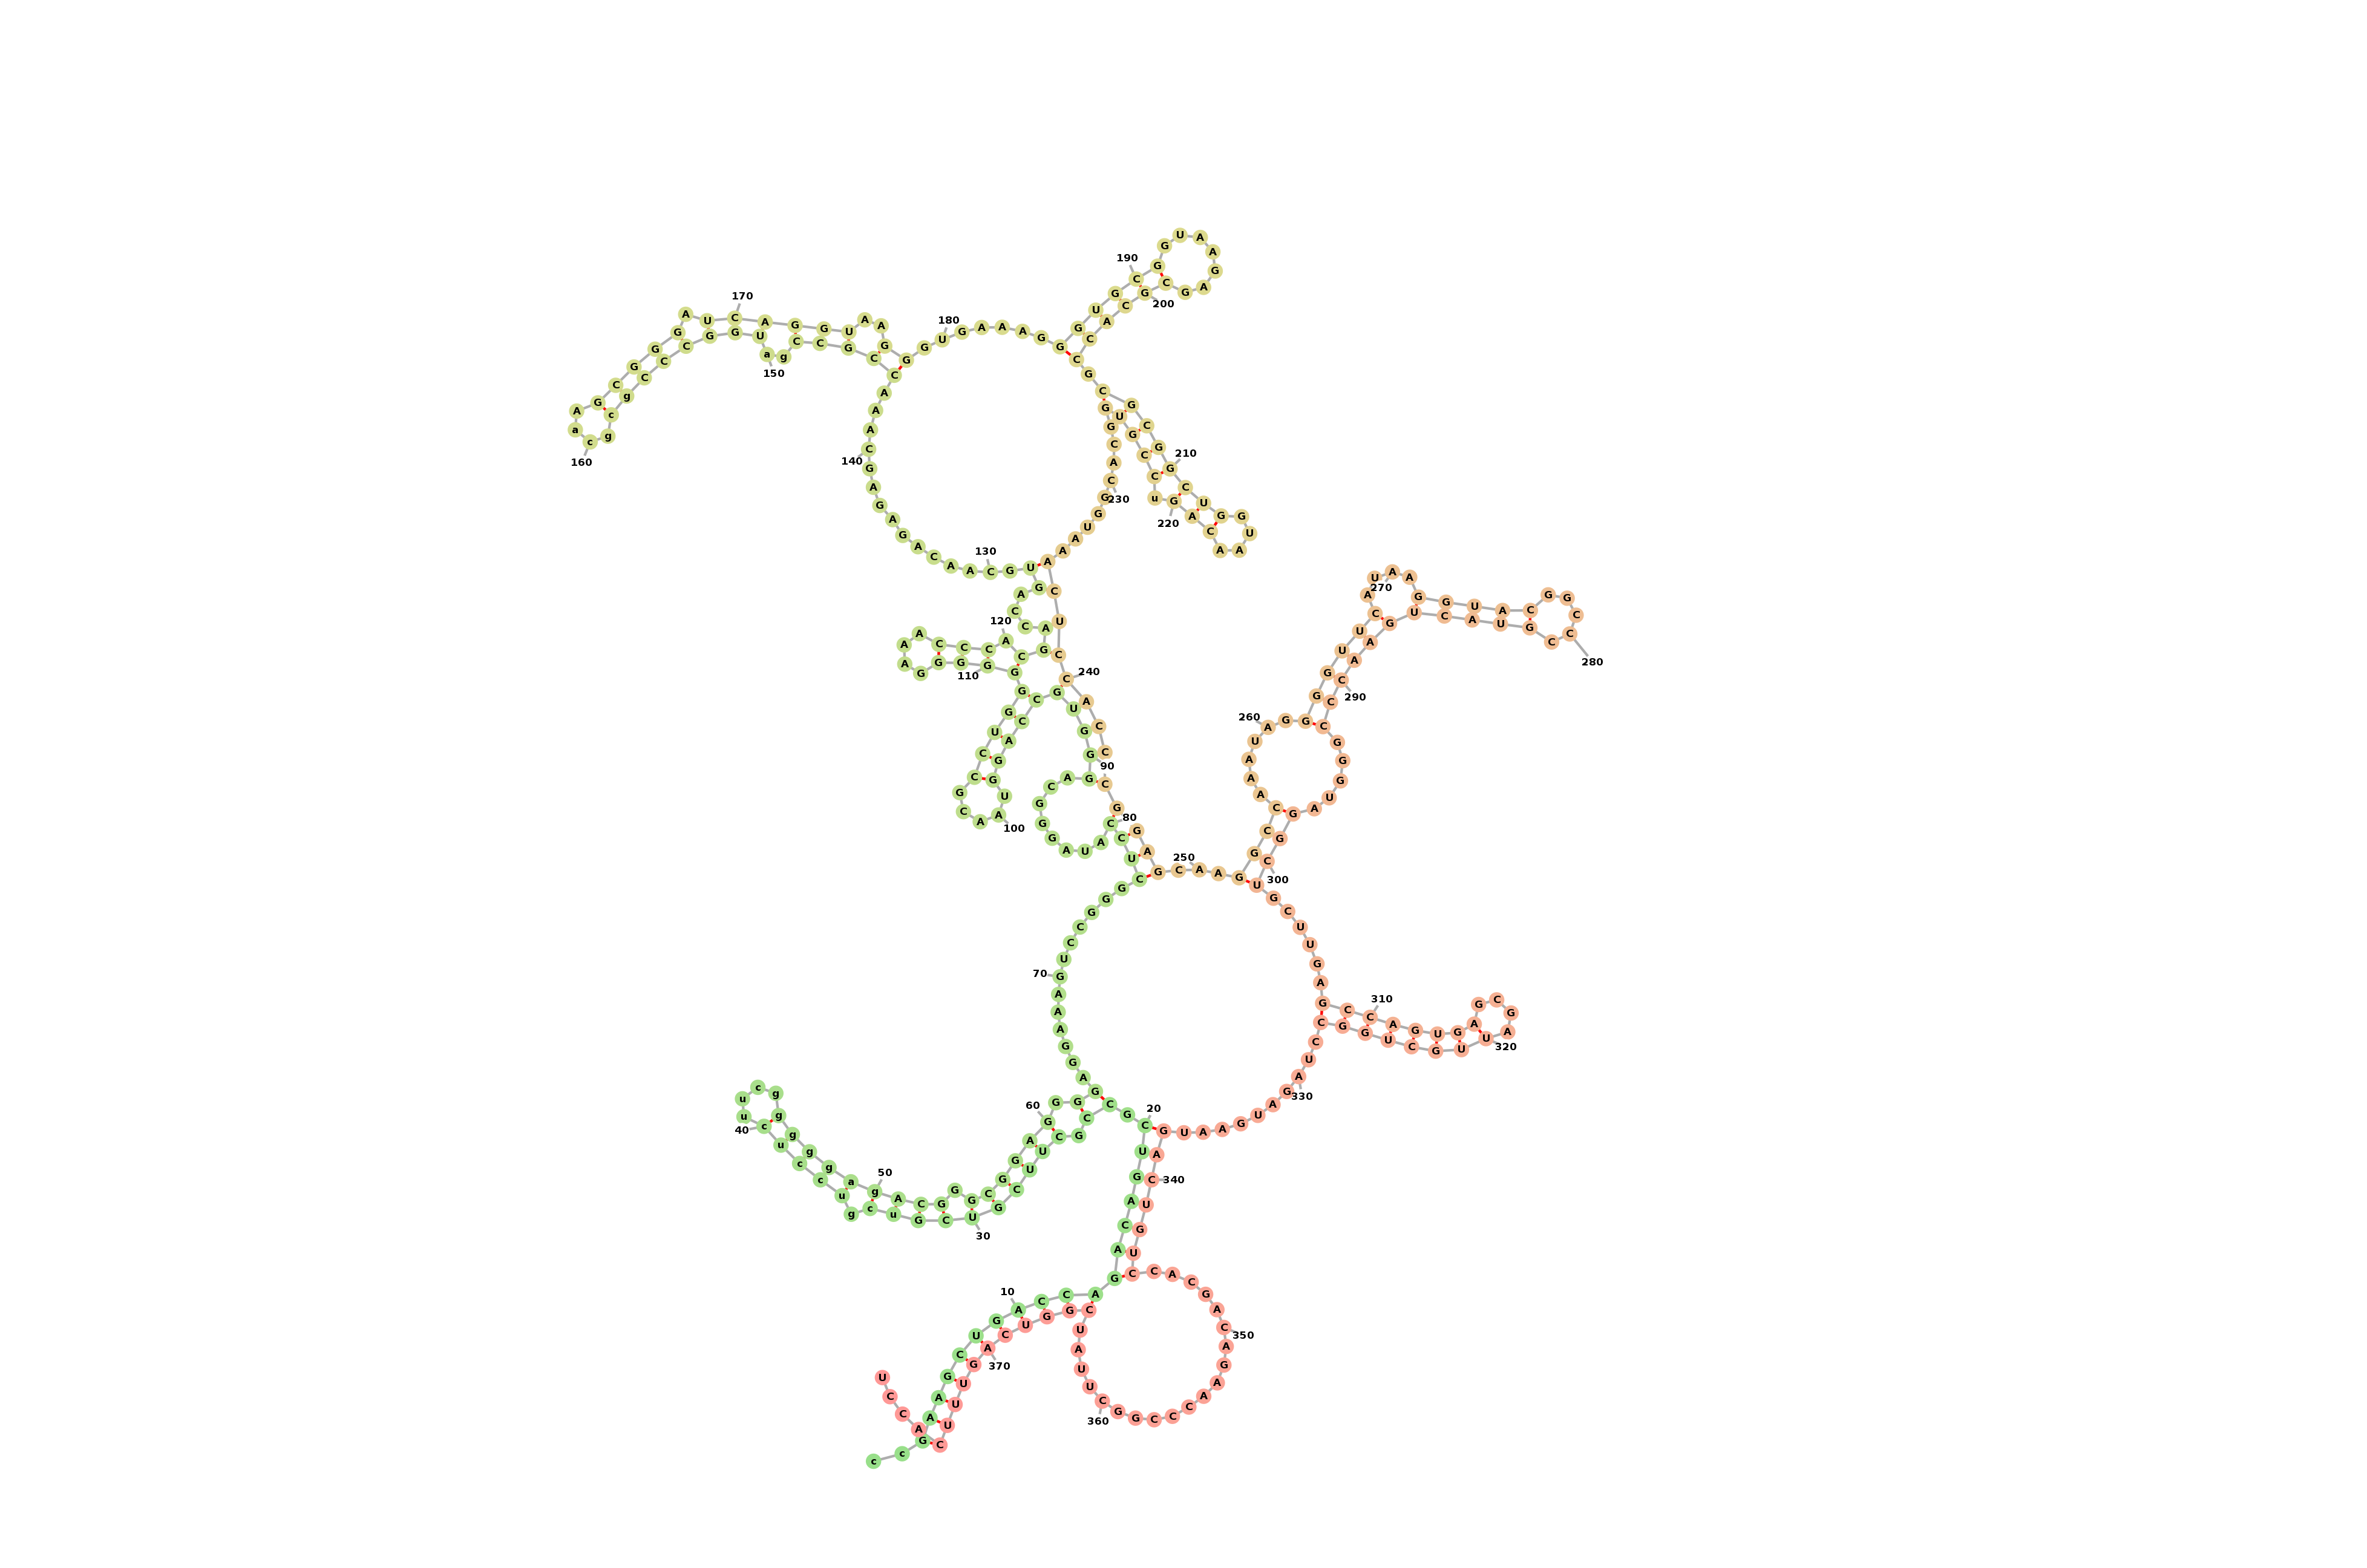
\includegraphics[width=0.5\textwidth]{./pictures/refStructure_pictures/CP001509-3-functional.png} \\
\end{tabular}
\caption{{\bf reference structures for RNA families.} Visualization with program forna \cite{forna} }
\label{table:reference structures}
\end{table}




\FloatBarrier

\subsection{\texttt{Kinwalker} parameter description} \label{kinwalker parameter description}

For fine tuning of the \texttt{Kinwalker} algorithm following parameters
are available: (1) \texttt{--transcription\_rate}, (2)
\texttt{--barrier\_heuristic}, (3) \texttt{--dangle}, (4)
\texttt{--maxkeep}, (5) \texttt{--grouping}, (6) \texttt{--lookahead}, (7)
\texttt{--nolonely}, (8) \texttt{--windowsize}, (9)
\texttt{--transcribed}. For my parameter space analysis, only transcription
rate, barrier heuristic, dangle and max keep were used and described below.
 



\subsubsection{transcription rates}

Number of nucleotides transcribed by the RNA polymerase per
second. Typically values for the speed of the transcription process in
nature are 10-20 nt per second for eukaryotes, 20-80 nt per second for
bacteria and about 200 nt per second for
bacteriophages\cite{transcriptionrates}.


\texttt{Kinwalker} approaches the problem with transcription rates with energy
barriers.
In the program \texttt{Kinwalker} the transcription rate influences the
refolding behaviour of an RNA sequence during transcription.
%to calculate refolding between structures.
To get from the current $s_{i,j}$ structure to the $s_{i,j+1}$ structure
\texttt{Kinwalker} estimates an energy barrier, which has to be overcome in order to
refold to the $s_{i,j+1}$ structure. This energy barrier is equivalent to
chemical kinetics activation energies (fig.~\ref{fig:energyBarrier}).
Transforming, i.e. adding or deleting substructures backtracked from the $C$ matrix, consumes time. If \texttt{Kinwalker} tries to insert a new substructure, the corresponding energy barrier is checked if such insertion could be even possible within the given time. If the energy barrier was to high, and therefore the time was to short, this specific substructure cannot be inserted and another one is tried.
 
Transcription rates, ranging from 10 to 500 nucleotids per second (nt/s) with 10 nt/s steps, were used for this \texttt{Kinwalker} parameter space analysis.
 
\begin{figure}
  \centering
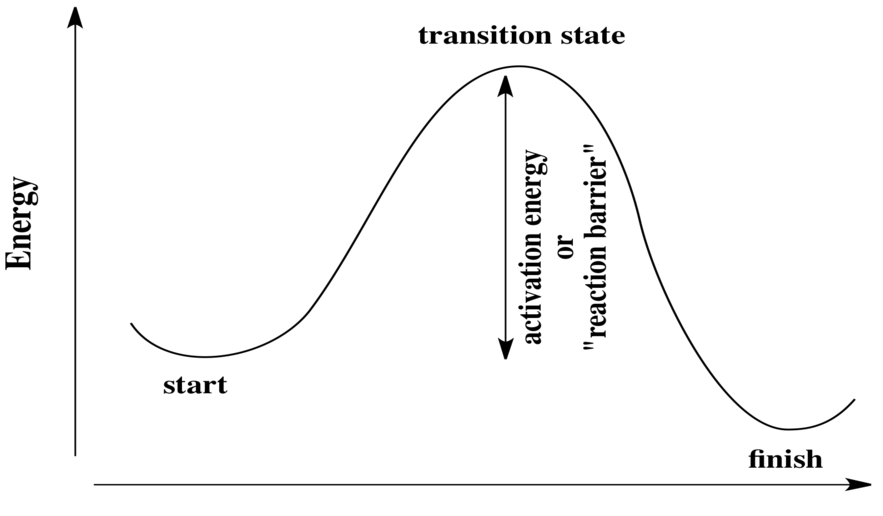
\includegraphics[width=0.5\textwidth]{./pictures/energyBarrier.png}
\caption{{\bf Kinetic model of activation energy.} To compare with RNA energy barriers, start and end are here seen as RNA structures, energy is the free energy of an RNA structure and the \texttt{Kinwalker} energy barrier is pictured as activation energy.}
\label{fig:energyBarrier}
\end{figure}
 
\FloatBarrier
\subsubsection{Barrier heuristic}

\texttt{Kinwalker} implements two direct path-finding algorithms, \texttt{Morgan$-$Higgs} and \texttt{findpath}. Both of these methods are heuristics, since the general problem of finding direct paths is \texttt{NP\_hard}\citep{manuch:2011}.
A direct path-finding algorithms can be described as follows:
Let A and B be structures of sequence S and $A_{bp}$, $B_{bp}$ their set of base-pairs. Overall $|BP_{distinct}|$ moves (i.e. adding or removing base-pairs) are necessary to transition from A to B.


\begin{equation}
BP_{distinct} = (A_{bp} \cup B_{bp}) \setminus (A_{bp} \cap B_{bp})
\label{eq:bpDistinct}
\end{equation}

The order of moves can be permuted, but some permutations lead to invalid routes, because adding a base-pair \textit{b} from B before removing a base-pair \textit{a} from A whereby \textit{a} and \textit{b} using the same base, is not possible. 

\texttt{Morgan$-$Higgs} and \texttt{findpath} algorithm are similar, but differ at
choosing the best path. \texttt{Morgan$-$Higgs} is based on minimal
collisions between A and B and \texttt{findpath} is based on minimal free energy
differences. Furthermore, \texttt{findpath} uses a breadth-first search, and is
therefore able to examine more than one solution path.


\paragraph{\texttt{Morgan$-$Higgs} \cite{morganhiggs}}

\texttt{Morgan$-$Higgs} uses the following heuristics procedure: 
\begin{enumerate}
\item Find the base-pair in B which has the least number of incompatible pairs in A. If more than one is found, choose randomly
\item Remove all incompatible pairs in A and add the base-pair from B to A
\item Intermediate structure A' arises
\item Save the energy of the maximum point reached during adding/removing
\item repeat from step 1 with A' until B is reached
\end{enumerate} 

The general assumption of this method is, that the path found using the
above procedure, has the lowest $h_{AB}$, where $h_{AB}$ is the minimal
energy value of $\Delta E_{AB}$ for all possible routes. $\Delta E_{AB}$
is the barrier between A and B. The energy barrier is the energy difference
between A and the A' with the maximum energy on the route towards B.

The \texttt{Morgan$-$Higgs} heuristics uses a greedy approach, i.e. it
chooses only one (the best) path and therefore often misses reasonable alternative solutions.

\paragraph{\texttt{findpath} \cite{Flamm:2000}}

In contrast to \texttt{Morgan$-$Higgs}, the \texttt{findpath} algorithm explores
several trajectories simultaneously. Starting from structure A, all
conformations that are one move closer to B are generated. Only the $m$
best paths are kept and serve as starting structures for the next
iteration. Here, a best path is the one with the smallest energy
barrier. This breadth-first search can be restricted by the parameter
\texttt{--maxkeep} ($m$) (fig.~\ref{fig:find-pathSearch}). In principle, setting a max-barrier height would allow for premature
termination of paths, if the path-energy is higher than the upper bound of
the barrier height. However, this function is not implemented in the
current version of the \texttt{findpath} heuristic.

\begin{figure}
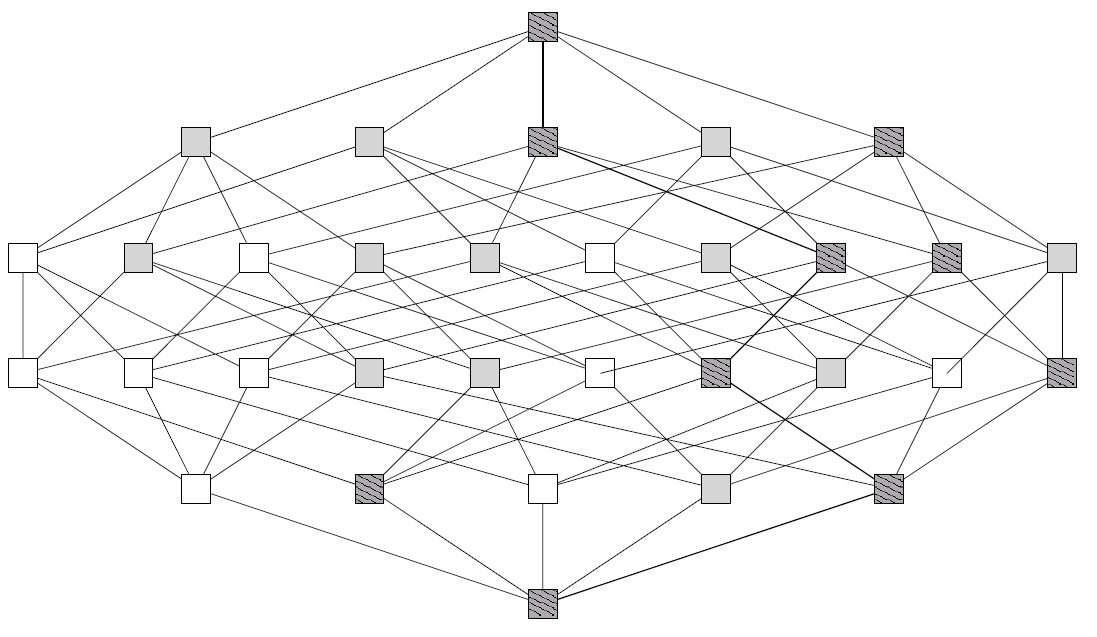
\includegraphics[width=0.6\textwidth]{./pictures/find-path.png}
\caption{{\bf Direct path-finding for two structures.} With \texttt{--maxkeep}=2 only striped structures are used to generate new conformations in the next iteration.}
\label{fig:find-pathSearch}
\end{figure}

\FloatBarrier
\subsubsection{Dangling ends}


Apart from the flexibility of the sugar-phosphate backbone and stability of
base-pairs, dangling end contributions and coaxial stacking of helices is important for RNA folding predictions\cite{walter:94}\cite{neilson:80}, since they decrease the free energy. Dangling is the effect of stacking an unpaired base to an adjacent helix. 


For better understanding of the dangling contribution, we assume that we
have a hairpin loop with a sequence \texttt{"GGGAAAACCC"} and add unpaired
bases to the sequence at the 3 and 5 prime end. Without dangling end
contribution, the free energy of the changed hairpin structure
\texttt{"UUGGGAAACCCC"} would be the same. Figure: \ref{fig:dangling} shows
this sample hairpin structure with U-U and C bases as possible dangling
ends. If dangling is considered, the unpaired bases are able to stack onto
their adjacent base-pairs, but do not form a pair with them. The 3 prime
dangling C stacks with the C-G base-pair and the adjacent 5 prime
dangling U can also stack with the C-G base-pair. This stapling result in a
noteworthy decrease of free energy\cite{walter:94}. Note, that the second
added U is not adjacent to the C-G base-pair, and therefore does not
contribute to the free energy of the RNA structure.

To use different dangling end approaches, 4 different dangle-models are implemented:

\begin{itemize}
	\item Dangle 0: dangling end energy contribution is not taken into account at all.
	\item Dangle 1: a single base is only allowed to stack onto one particular base-pair. If there is more than one possibility, the energetically lowest one is used.
	\item Dangle 2: if there are bases available for stacking, assume
          that every base is dangling on every possible base-pair. That
          means that the energy contribution of one dangling base may be added to more than one base-pair. Dangling can occur even if the dangling base is part of another base-pair. The idea behind this approach is the assumption that an RNA structure in equilibrium, is in constant flux between different conformations.
	\item Dangle 3: Coaxial stacking of multiloop stems is allowed, but
          dangling is regarded as in case 2 (dangle 1).
	
\end{itemize} 

\begin{figure}
	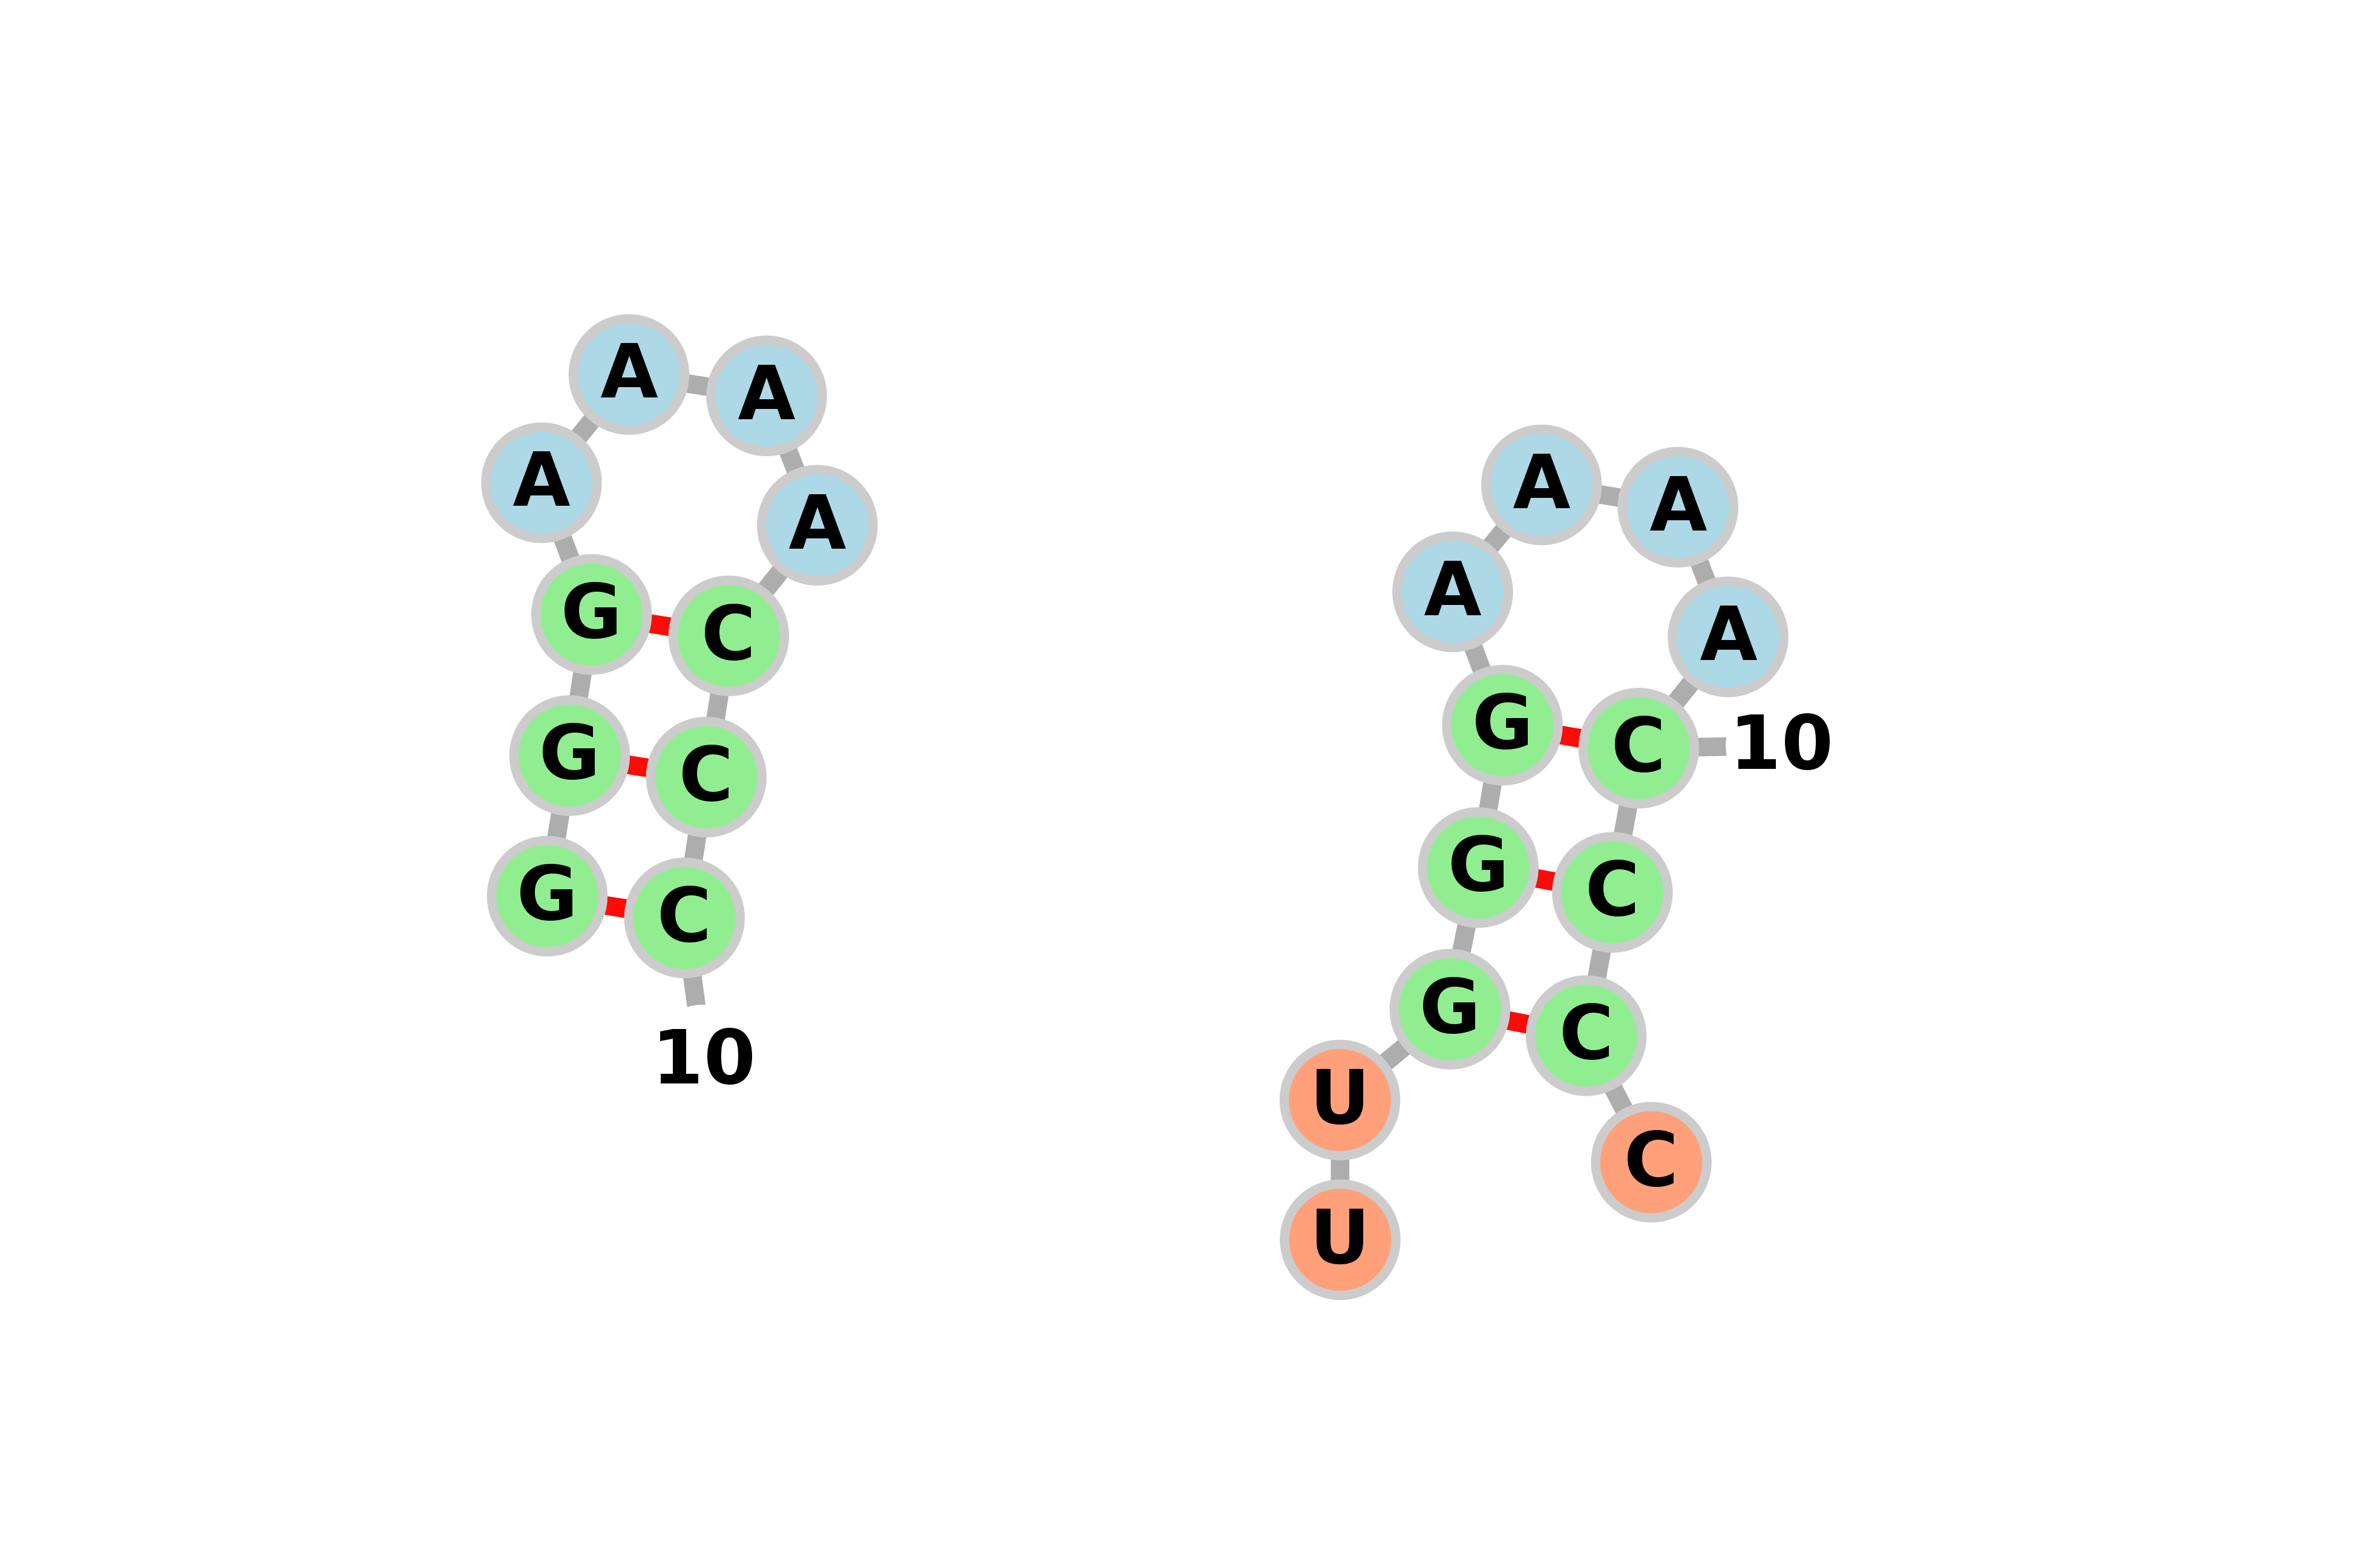
\includegraphics[width=0.6\textwidth]{./pictures/dangling/dangling.png}
	\caption{{\bf sample hairpin with and without dangling bases}
	Free energy of right hairpin is lower than left one, because adjacent bases U and C are able to stack onto the G-C base-pair and thus decreasing the free energy and stabilizing the hairpin even more. The second U is not able to stack, because it is not directly adjacent.}
	\label{fig:dangling}
\end{figure}


\FloatBarrier



\subsubsection{max keep}
Max keep parameter describes the maximal amount of paths $m$ for the \texttt{findpath} breadth-first implementation. Higher max keep could lead to better results, with the downside of a big increase in calculation time. If \texttt{Morgan$-$Higgs} algorithm is used, max keep parameter is not considered at all, because there is only one solution path.
 

\subsection{\texttt{Kinwalker} output}


Figure: \ref{fig:kinwalker output} shows a sample \texttt{Kinwalker} output file that summarizes the folding trajectory of an RNA sequence.
The first two lines define the RNA sequence, as well as the MFE structure of this RNA sequence. Each line also shows the free energy of this structure (here -60 kcal/mol, this is the MFE structure).
The last structure in the output again, shows the MFE structure and the last line shows the whole runtime of the algorithm.
In between, the whole folding trajectory is shown.
Every line shows (from left to right, separated with tabulators):
(1) the current formed structure in dot bracket format, (2) the free energy
of this specific structure, (3) overall passed time since the beginning of
transcription, (4) the energy barrier to get from the previous structure to
the current structure, (5) allowed max energy barrier, and (6) number of bases already transcribed.

\begin{figure}[ht] 
\centering
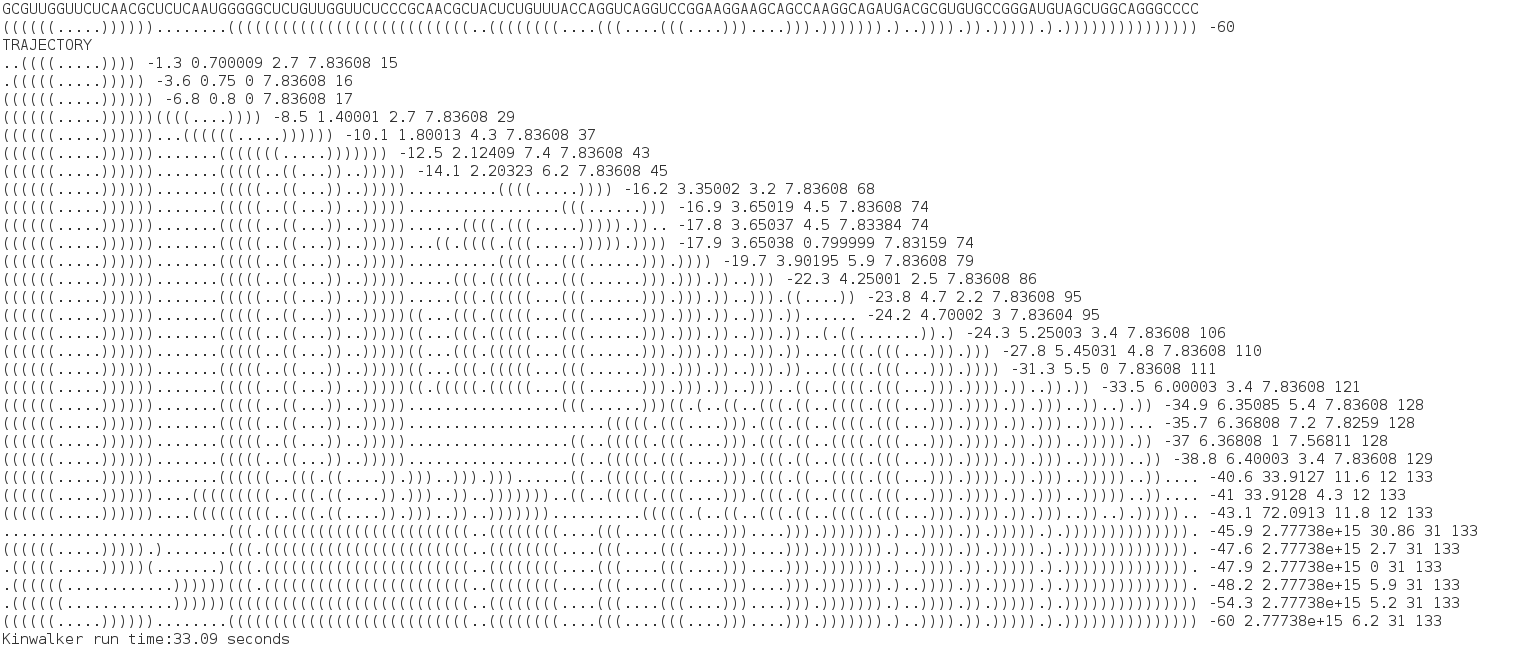
\includegraphics[width=1\textwidth]{./pictures/KinwalkOutput.png}
\caption{{\bf \texttt{Kinwalker} output file.}
Every line shows (from left to right, separated with tabulators):
(1) the current formed structure in dot bracket format, (2) the free energy
of this specific structure, (3) overall passed time since the beginning of
transcription, (4) the energy barrier to get from the previous structure to
the current structure, (5) allowed max energy barrier, and (6) number of bases already transcribed.
}
\label{fig:kinwalker output}
\end{figure}
\FloatBarrier


\section{evolution of input data and predictions} \label{section:scores}

For evaluation of \texttt{Kinwalker} output data, different scoring functions were used, statistically analysed and the results were plotted for better visualization, using  \texttt{ggplot2}\citep{ggplot2} and  \texttt{R}\citep{R}. The source code for scoring functions was implemented in  \texttt{Python}\cite{python}. 
Computations were performed on a 64-bit machine with Intel Octacore i7-4771 3.50 GHz and 32 GB RAM.

The scores used in this thesis are separated into two sections, the input scores \ref{section:input scores} and the prediction scores \ref{section:prediction scores}.
Input scores are dealing with the input data itself, like RFAM alignments and the evolutionary conservation of their sequences. Prediction scores are dealing with \texttt{Kinwalker} output data and statistically evaluation of co-transcriptional folding trajectories.  

\subsection{input scores} \label{section:input scores}

\subsubsection{structure conservation index (SCI)\cite{Washietl:2005} and consensus structure}
			
The SCI is used to measure evolutionary conservation of Alignment $A$
consisting of ${|A|}$ individual sequences $a$.
SCI compares the free energy of the alignment consensus structure to the
mean single sequence energies (i.e. the MFE for each sequence in the
alignment). The consensus structure is the minimum free energy structure of
an alignment, which can be formed by all sequences. Figure:
\ref{fig:consensusStructure_example} shows the output of a consensus
structure for a given example alignment. Let's take a random base-pair
(G-C) predicted in the consensus structure. There is no guaranty that all
of the sequences are forming the same base-pair at this position, or
forming a base-pair at all. To highlight this behaviors a color code is
used for the consensus structure representation (fig.~\ref{fig:colorCode}). A
conserved pair with identical pairing bases in coloured in red. All the other colors indicate compensatory mutations i.e. a nucleotide mutation with no loss in structure and functionality, for example the mutation from a G-C base-pair to a A-U base-pair. Pale colors indicate if some sequences cannot form this base-pair at all. Keeping this code in mind, a blue region indicated a higher structure conservation (due to compensatory mutations) than a red region.

\begin{figure}[ht] 
\centering
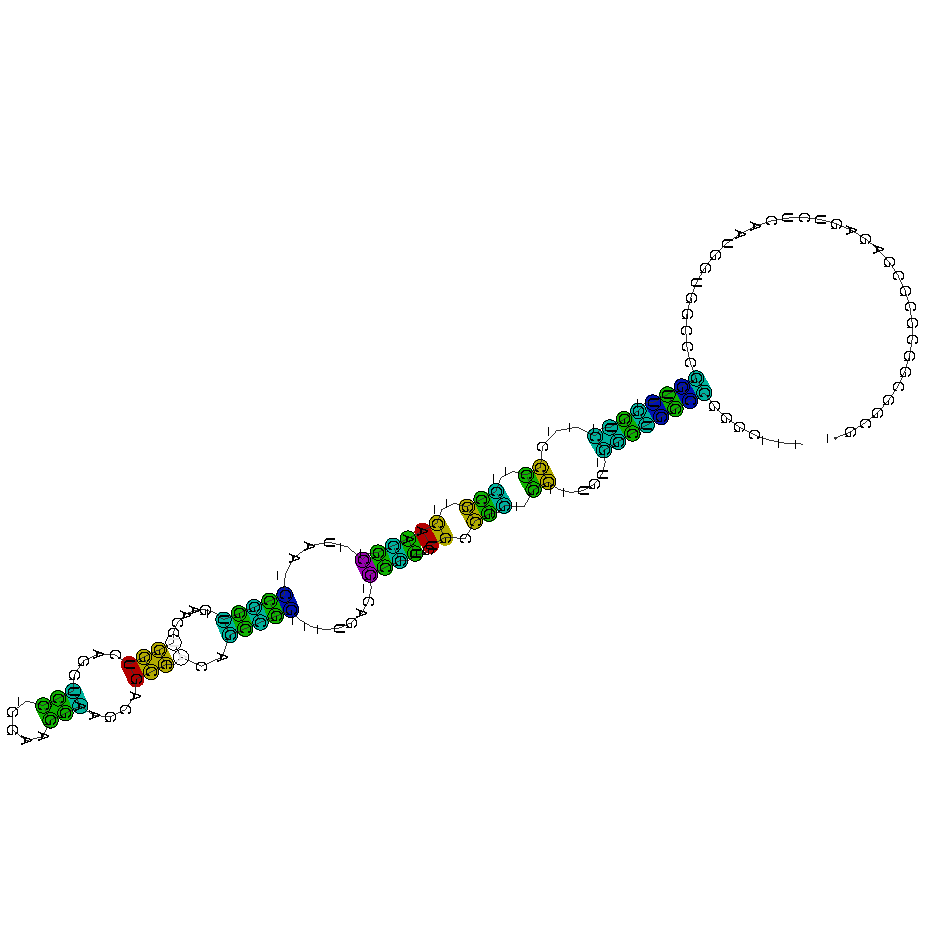
\includegraphics[width=0.7\textwidth]{./pictures/consensusStructure/SRP.pdf}
\caption{{\bf consensus structure}
consensus structure representation for a given example alignment.
A color code defines the amount of possible base-pairs at a given location.
}
\label{fig:consensusStructure_example}
\end{figure}

\begin{figure}[ht] 
\centering
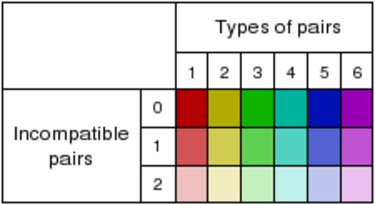
\includegraphics[width=0.5\textwidth]{./pictures/consensusStructure/colorcode.pdf}
\caption{{\bf consensus structure color code}
color representation of compensatory mutations: 
(i): different colors indicate the amount of different base-pairs that are formed in the alignment sequences: red = only one base-pair in all sequences, pink = 6 different base-pairs are possible here
(ii): intensity of the color indicates how many sequences cannot form a base-pair at this location
}

\label{fig:colorCode}
\end{figure}




\begin{equation}
SCI(A) = MFE(\mbox{consensus structure}) \cdot \frac{1}{\frac{1}{|A|}\cdot \sum\limits_{a\in A} MFE(a)}
\label{structure conservation index}
\end{equation}

SCI of $0$ means, that no consensus structure was found for this alignment. SCI of 1 means, that this alignment correspond to perfect structure conservation. SCI, consensus structure and the corresponding consensus free energy is calculated via RNAalifold\cite{RNAalifold} from the ViennaRNAPackage 2.0\cite{ViennaRNA}.


\subsubsection{sequence similarity}
	

Sequence similarity is a simple percentage based measure to calculate nucleotide similarity
between two aligned RNA sequences $S_1$ and $S_2$.

\begin{equation}
\mbox{sequence similarity($S_1,S_2$)} = \frac{1}{n}\cdot \sum\limits^n_{i=1} \begin{cases} 
1 & \mbox{if } S_1[i]=S_2[i] \\
0 & \mbox{if } S_1[i]\not=S_2[i] \\ \end{cases}
\label{eq:sequence similarity score} 	
\end{equation}

Where $n$ is the number of all bases and gaps for a sequence.
Results ranges from 0-1. Similarity of 1 means that the sequences are identical. 

Furthermore the mean distance similarity can be used, to determine the mean base-pair distance of all sequences of an alignment $A$ to a given reference sequence $S_{ref}$. 
				 
\begin{equation}
 \mbox{mean distance similarity} =  \frac{1}{n}\cdot \sum\limits^n_{i=1} \mbox{sequence similarity($S_{ref}$,$S_i$)}
 \label{eq:sequence similarity average}	
\end{equation}

Where n is the amount of all alignment sequences in $A$, and $S_i$ is one of these sequences.
Results range from 0-1. Mean distance similarity of 1 means, that every $S_i$ is identical with $S_{ref}$.

\subsection{prediction scores} \label{section:prediction scores}

\subsubsection{base-pair diversity} 

Base-pair diversity is used to determine how many different base-pairs a
sequence of length $n$ forms during and after co-transcriptional folding, and how many
could have been formed theoretically ($maxBP$).
\begin{equation}
maxBP= \frac{(n\cdot(n-1))}{2}
\label{eq:maximal base-pairs}
\end{equation}


For a particular folding trajectory $M$ with an unique set of base-pairs $BP(i,j)$ (multiple occurrences of base-pair $(i,j)$ are not taken into account),

\begin{equation}
bpDiversity(M) = \frac{1}{maxBP}\cdot \sum\limits_{(i,j) \in \texttt{M}} 
\begin{cases} 1 & \mbox{if  (i,j) has been formed} \\ 
0 & \mbox{if  (i,j) has not been formed} \\ 
\end{cases}
\label{eq:base-pair diversity}
\end{equation}
 
Here a higher score means that more diverse sets of base-pairs are formed
during folding of the RNA sequence.  


The score can be extended by adding a time factor into the
calculations. Base-pair diversity now considers the overall lifetime of one
base-pair. A short-lived base-pair now gets a lower score, than a base-pair
which was longer stable during RNA folding event. This score decreases the
bias with short-lived base-pairs which would otherwise get the same score
as long-lived base-pairs. If existence time of $(i,j)$ should be considered, the time quotient $\frac{\Delta Time_{ij}}{T_{total}}$ has to be
inserted into the formula.

\begin{equation}
bpDiversity_{\Delta Time_{ij}}(M) = \frac{1}{maxBP}\cdot \sum\limits_{(i,j) \in M} 
\begin{cases} \frac{\Delta Time}{T_{total}} & \mbox{if  (i,j) has been formed} \\ 
0 & \mbox{if  (i,j) has not been formed} \\ 
\end{cases}
\label{eq:base-pair diversity time depended}
\end{equation}	

Here $\Delta Time_{ij}$ is the existence time of base-pair $(i,j)$ during the whole
RNA folding event. Here the existence times of multiple occurrences of $(i,j)$ are taken into account and are simply summed up.
$T_{total}$ is the time from transcription start until the RNA is fully transcribed, has successfully
folded into the MFE structure and therefore has reached the equilibrium
state. $\frac{\Delta Time_{ij}}{T_{total}}$ is proportional to the probability to observe base-pair (i,j) along the trajectory to its MFE structure.

Generally speaking, a high $bpDiversity_{\Delta Time_{ij}}$ means that more diverse base-pairs are formed during
the folding process. However, RNAs with fewer different base-pairs, but
longer existence time will also result in a high $bpDiversity_{\Delta Time_{ij}}$. 

Likewise, low $bpDiversity_{\Delta Time_{ij}}$ indicates fewer different base-pairs and/or shorter existence
time of base-pairs.

			
Furthermore, to get an overall view of the behavior of alignment sequences, a mean base-pair diversity score for alignment $A$ can be
calculated.  Mean base-pair diversity allows to compare different RNA
families and their sequence alignments.

\begin{equation}
meanBpDiversity(A) = \frac{1}{|A|}\sum\limits_{a \in A} bpDiversity(a)_{\Delta Time_{ij}}
\label{eq:time depended base-pair alignment diversity}
\end{equation}
	
Where $A$  is a set of all sequences $a$ in the alignment. High scores suggest, that alignment sequences are forming a more diverse sets of base-pairs.

							
\FloatBarrier	


\subsubsection{Ensemble diversity}	
		
Another score to assess the diversity of folding trajectories
can be derived from the ensemble diversity $<d>$ \cite{dissRonny}, i.e. the
weighted average distance between structures $s$ and $t$ in equilibrium.
\begin{equation}
<d> = \sum\limits_{s,t} p(s) \cdot p(t) \cdot d(s,t) 
\label{eq:ensemble diversity original}
\end{equation}

where $p(s)$ is the probability to observe structure $s$ in the Boltzmann
ensemble, $p(t)$ is probability to observe structure $p$ and $d(s,t)$ is
the bp distance between structures $s$ and $t$.  Since we use the bp
distance as distance measure in the above equation, we can also express
equation: \ref{eq:ensemble diversity original} in terms of equilibrium bp
probabilities: \cite{EnsembleDistance}

\begin{equation}
<d>=\sum\limits_{i,j} p(i,j)\cdot(1- p(i,j))
\end{equation}

The largest contributon of a pair $(i,j)$ to this sum is obtained, if
$p(i,j)=0.5$.
In order to compare ensemble diversities for different RNAs,
$<d>$ can be normalized through dividing by the sequence length.

However, we are interested in the diversity of base-pairs along the folding
trajectory $M$, not the diversity of the entire ensemble of
structures. Therefore, we use the probability to observe a bp along the
folding trajectory $M$ instead of equilibrium probabilities. 
As a consequence, we use the fraction of observing bp $(i,j)$ within a
time interval (here named period) as probability to observe bp $(i,j)$.

The probability of base-pair (i,j) to appear is then $\frac{\Delta Time_{ij}}{period}$, where $\Delta Time_{ij}$ is the existence time of base-pair
(i,j) during the checked period. By substituting $p(i,j)$ with time
periods, we get

\begin{equation}
\mbox{ensemble diversity(period)} = \frac{1}{l} \cdot \sum\limits_{i,j} (\frac{\Delta Time_{ij}}{period})\cdot (1- \frac{\Delta Time_{ij}}{period})  
\label{eq:ensemble diversity }
\end{equation}

After the last step of transcription, the RNA has not necessarily reached
the equilibrium state yet and folding continues.

In the following, I consider periods ranging from $2\times$transcription time over
$5\times$transcription time, to $10\times$transcription time, with
\begin{equation}
  transcription\ time = {sequence\ length} / {transcription\ rate}.
\end{equation}

If diversity increase happens with $10\times$transcription time but not with $2\times$ or $5\times$ transcription times, this suggest that refolding into the
MFE starts extremely late. I expect such behavior in cases where the RNA
got stuck in a stable local energy minimum. If there is no diversity difference between
$2/5/10\times$ transcription times, than refolding either happens shortly
after finished transcription, or very late after transcription i.e. after
$10\times$ transcription time.


If \ref{eq:ensemble diversity } is high, the folding trajectory is more diverse. Max value is obtained, if all base-pairs have a probability of 50 \% to exist. If all base-pairs stay the same over folding, the ensemble diversity is zero (extremely low diversity).
If the ensemble diversity becomes significantly higher when larger time periods are
used, then the folding trajectory is more diverse at the later steps.


\subsubsection{Ensemble Distances \cite{EnsembleDistance}}
Next, we want to analyze whether a substructure
of the reference structure $s_{ref}$ is part of the folding trajectory $M$.
Therefore, we use the simple ensemble distance $d_E(M,s_{ref})$, which measures
the percentage of $(i,j) \in s_{ref}$ found in $M$.
%the base-pair distance from a reference structure $s_{ref}$ to all
%structure $s_M \in M$.

\begin{equation}
d_E(M,s_{ref}) = \frac{1}{|s_{ref}|} \cdot \sum\limits_{(i,j) \in s_{ref}}
\begin{cases} 
1 & \mbox{if }(i,j) \in \texttt{M} \\ 
0 & \mbox{if }(i,j) \notin \texttt{M} \\
\end{cases}
\label{eq:SimpleEnsembleDistance}			
\end{equation}



%To determine whether the set of base-pairs
%$BP_{ref}$ of a reference structure $s_{ref}$ are part of the folding
%trajectory $M$ of a sequence $s$, i.e. if $s_{ref}$ is an intermediate
%structure of $M$, the simple ensemble distance $d_E$ can be used. 

%This score determines how many base-pairs of $s_{ref}$ are found in $M$ and results with the base-pair percentage of $S_{ref}$ in $M$.
If the own MFE structure is chosen as $S_{ref}$, folding traps can be detected.

%Here $(i,j)_{ref}$ is a base-pair $(i,j)$ found in $BP_{ref}$.
Multiple occurrences of $(i,j)\in s_{ref}$ in $M$ are no taken into account.
Due to normalization by dividing by $|s_{ref}|$ - every result ranges from
0 to 1.
$d_E(M,s_{ref})$ of 1 means that every $(i,j) \in s_{ref}$ was also formed in $M$.


The score can be extended by adding a time factor and the probabilities of all possible base-pairs into the
calculations. Ensemble distance $d_{E,T}$ now considers the overall lifetime of one
base-pair. A short-lived base-pair now gets a lower score, than a base-pair
which was longer stable during RNA folding event. The improved ensemble distance is now the expected distance between the predicted trajectory and the reference structure\cite{EnsembleDistance}.
Thus
\begin{equation}
d_{E,T}(M,s_{ref})= \sum\limits_{(i,j)_M \in s_{ref} } (1- p(i,j)) + \sum\limits_{(i,j)_M \notin s_{ref}} p(i,j),
\label{eq:ensemble distance}
\end{equation}

where $(i,j)_{M}$ is a base-pair $(i,j)$ present in $M$ and $p(i,j) =
\frac{\Delta Time_{ij}}{T_{total}}$, is the probability of appearance of
$(i,j)_{M}$. $\Delta Time_{ij}$ is the existence time of base-pair $(i,j)_{M}$ during the whole RNA folding event. The existence times of multiple occurrences of $(i,j)_{M}$ are simply summarized. $T_{total}$ is the time until the RNA is fully transcribed and has successfully folded into the MFE structure.


For comparison of sequence alignments, the average ensemble distance can be
calculated as well. The base-pair distance of an alignment $A$ with $|A|$
sequences $a$ to $s_{ref}$ can be used to detect evolutionary conserved
folding pathways. Trajectories of sequences with small evolutionary
distance should theoretically display similar folding patterns and
therefore show a lower average Ensemble Distance to $s_{ref}$. This,
however, is only true if $s_{ref}$ or substructures of it are known to be part of the
trajectory
i.e. $s_{ref}$ is an intermediate structure necessary for the
correct folding pattern.

\begin{equation}
\mbox{average Ensemble Distance} = \frac{1}{|A|} \sum\limits_{a\in A} d_E(M_a,s_{ref})
\label{eq:meanEnsembleDistance}	
\end{equation}

Here, $M_a$ is the trajectory of $a$. Division by $|A|$ results in a
normalized score between $0-1$.
Average Ensemble Distance = 1 if every base-pair in $s_{ref}$ is also
formed in every trajectory of $A$.


% ==================================================

\chapter{Results}

% ==================================================



\texttt{Kinwalker} data, calculated via scores shown in section "used
statistically scores"~\ref{section:scores} are plotted in this chapter to
visualize statistical dependencies. Data were computed with the statistics
program \texttt{R}\cite{R} and afterwards plotted with the \texttt{ggplot2} package
\cite{ggplot2}. This chapter is separated into different sections, each
dealing with one group of scoring function.
	
\section{structure conservation index (SCI), average sequence similarity}

The sequence similarity of each alignment sequence to their reference sequence as well as their consensus structure are shown in figure: \ref{fig:sequence_similarity}. 
\texttt{RNaseP} (\textit{RF00010}) shows the highest
average sequences similarity of 89.1 \% (fig.~\ref{fig:sequence_similarity} c) with a SCI of 0.7854, whereas
sequences of \texttt{SRP} RNA (\textit{RF00169}, fig.~\ref{fig:sequence_similarity} a) and \texttt{trpL} (\textit{RF00513}, fig.~\ref{fig:sequence_similarity} b) are
more dissimilar (mean sequence similarity: 68.2 \%, SCI: 0.8379 and 65.8
\%, SCI: 0.5312, respectively).

To calculate the SCI of an alignment, \texttt{RNAalifold} algorithm\cite{RNAalifold} was used.
%Table: \ref{fig:compare_SCI_sequence_similarity} shows the sequence similarity and the structure conservation index in comparison. 
Alignment \texttt{SRP} is the evolutionary most conserved alignment.
Although \texttt{RNaseP}  sequences show a higher sequence similarity than
\texttt{SRP} RNAs, their SCI is lower than the one of \texttt{SRP}
RNAs.
If the SCI is high but the average sequence similarity is low, a lot of
compensatory mutations have occurred during evolution and conserved the
functional structure.




%- CHECK,general explaination about evolutionary structure conservation,
%- CHECK,compensatorische mutationen ( color code, basenpaarungen sind konserviert)
%- CHECK, Structure conservation index for SRP,trpL,RNaseP .ps

%- Discussion:
%Where are important domains, therefore the structure more consrverd there,
%- and so on


\begin{figure}
\begin{tabular}{l|l}
(a) \texttt{SRP} (RF00169) \\
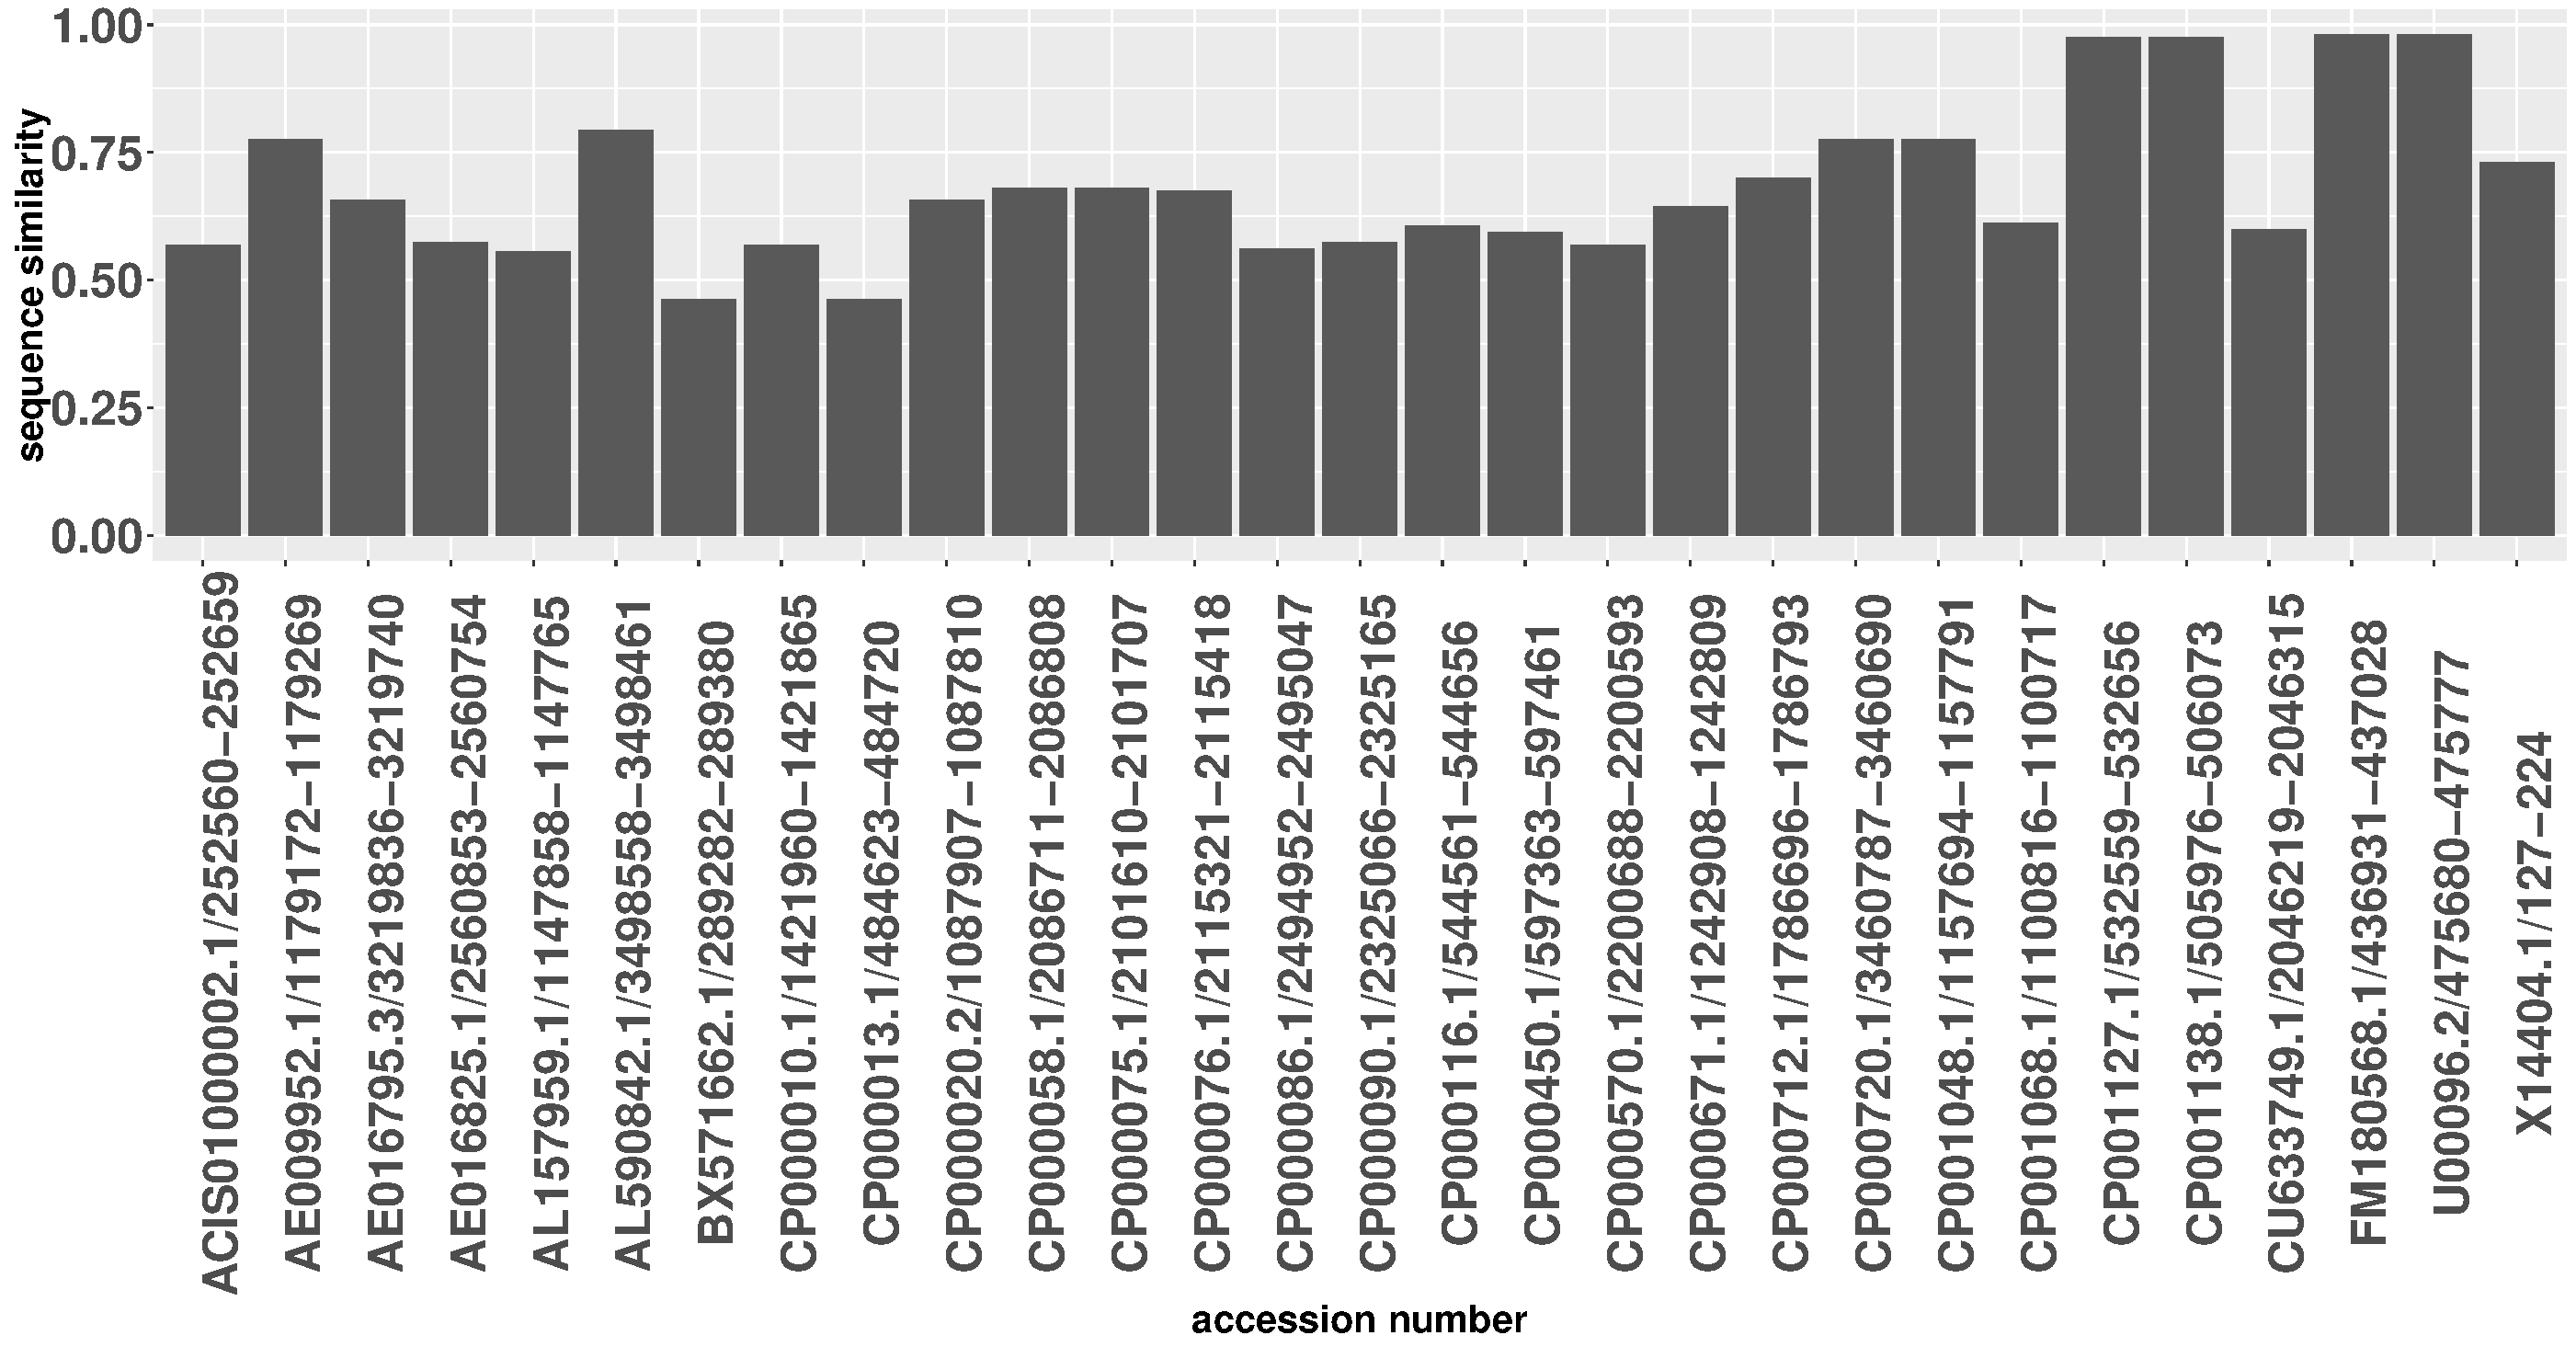
\includegraphics[width=0.5\textwidth]{./pictures/sequenceSimilarity/SRP.pdf} &
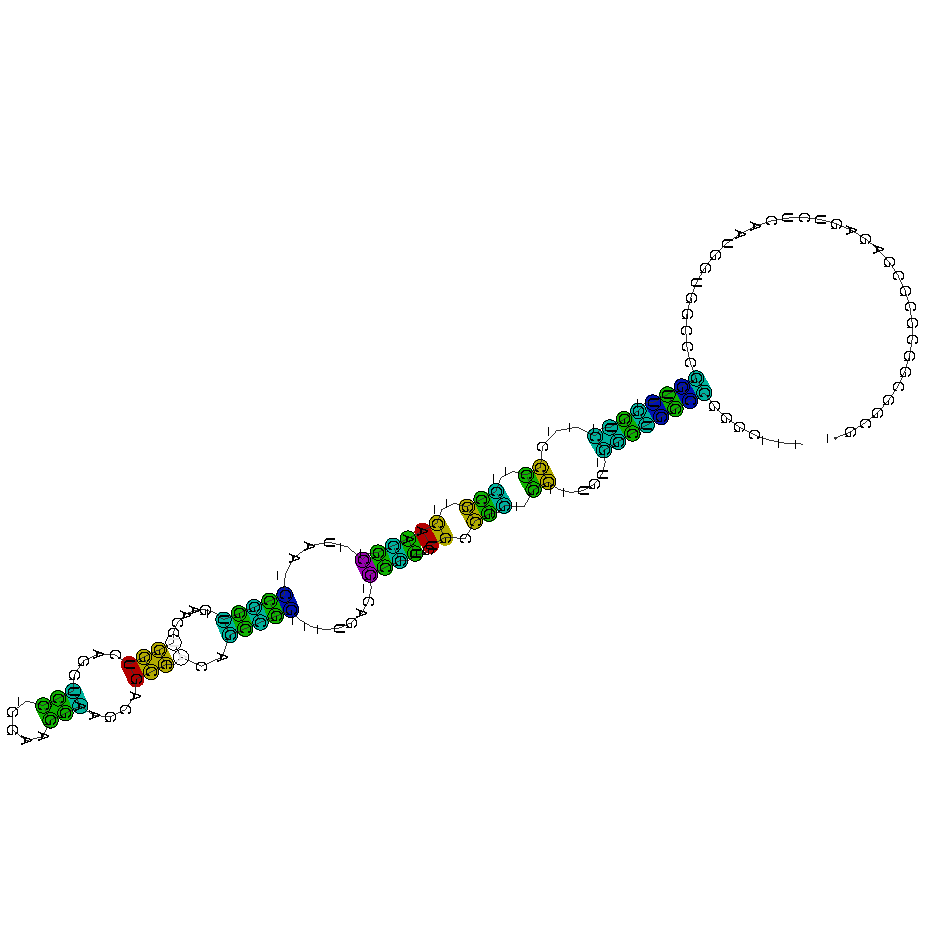
\includegraphics[width=0.4\textwidth]{./pictures/consensusStructure/SRP.pdf} \\

\hline
(b) \texttt{trpL} (RF00513) 
\\ 
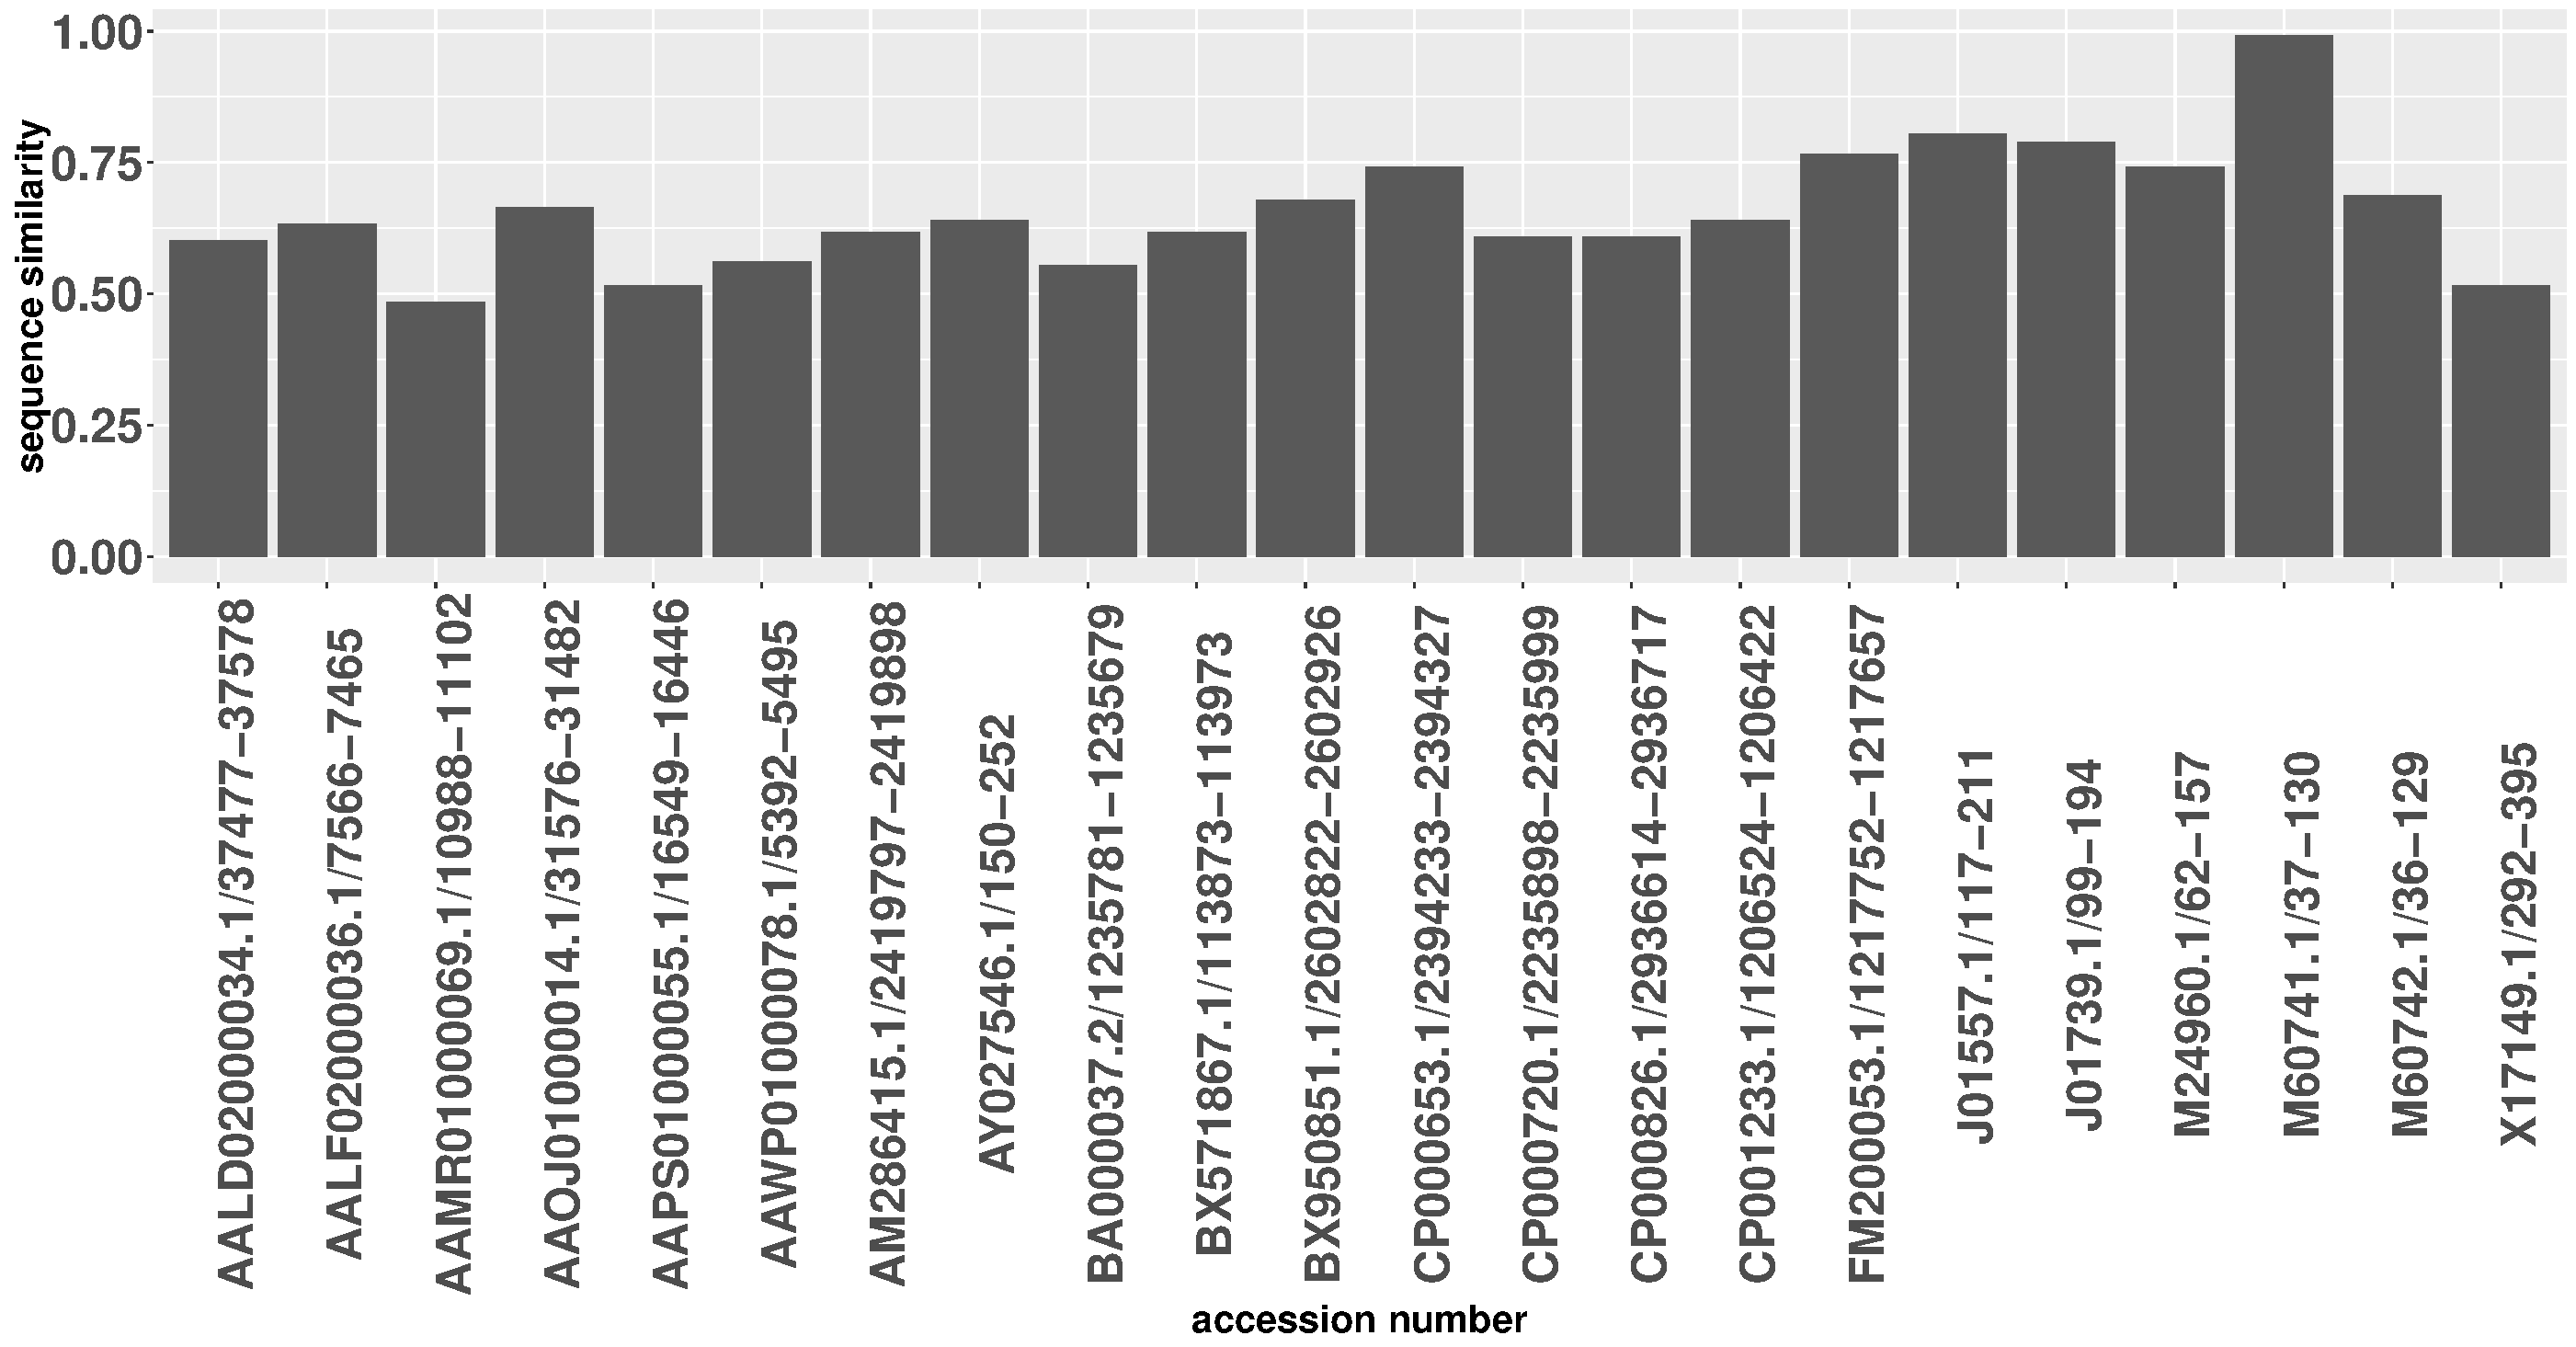
\includegraphics[width=0.5\textwidth]{./pictures/sequenceSimilarity/trpL.pdf} &
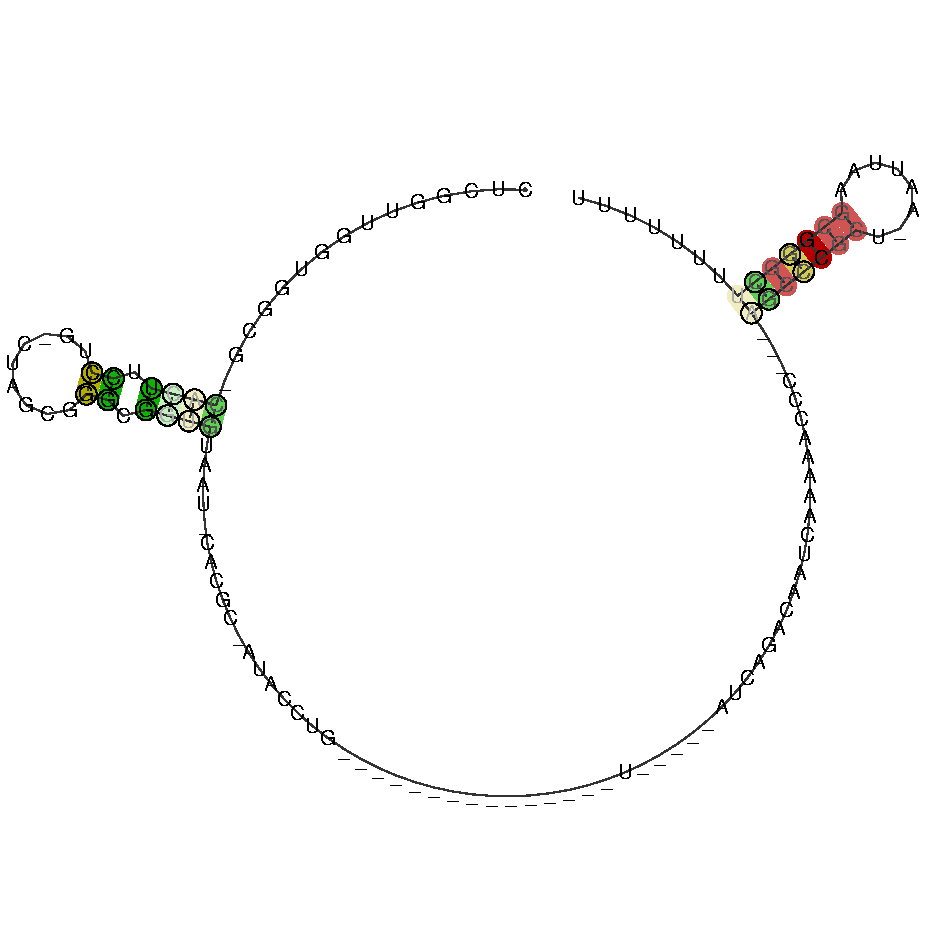
\includegraphics[width=0.4\textwidth]{./pictures/consensusStructure/TRP.pdf} \\
\hline
(c) \texttt{RNaseP} (RF00010)
\\
 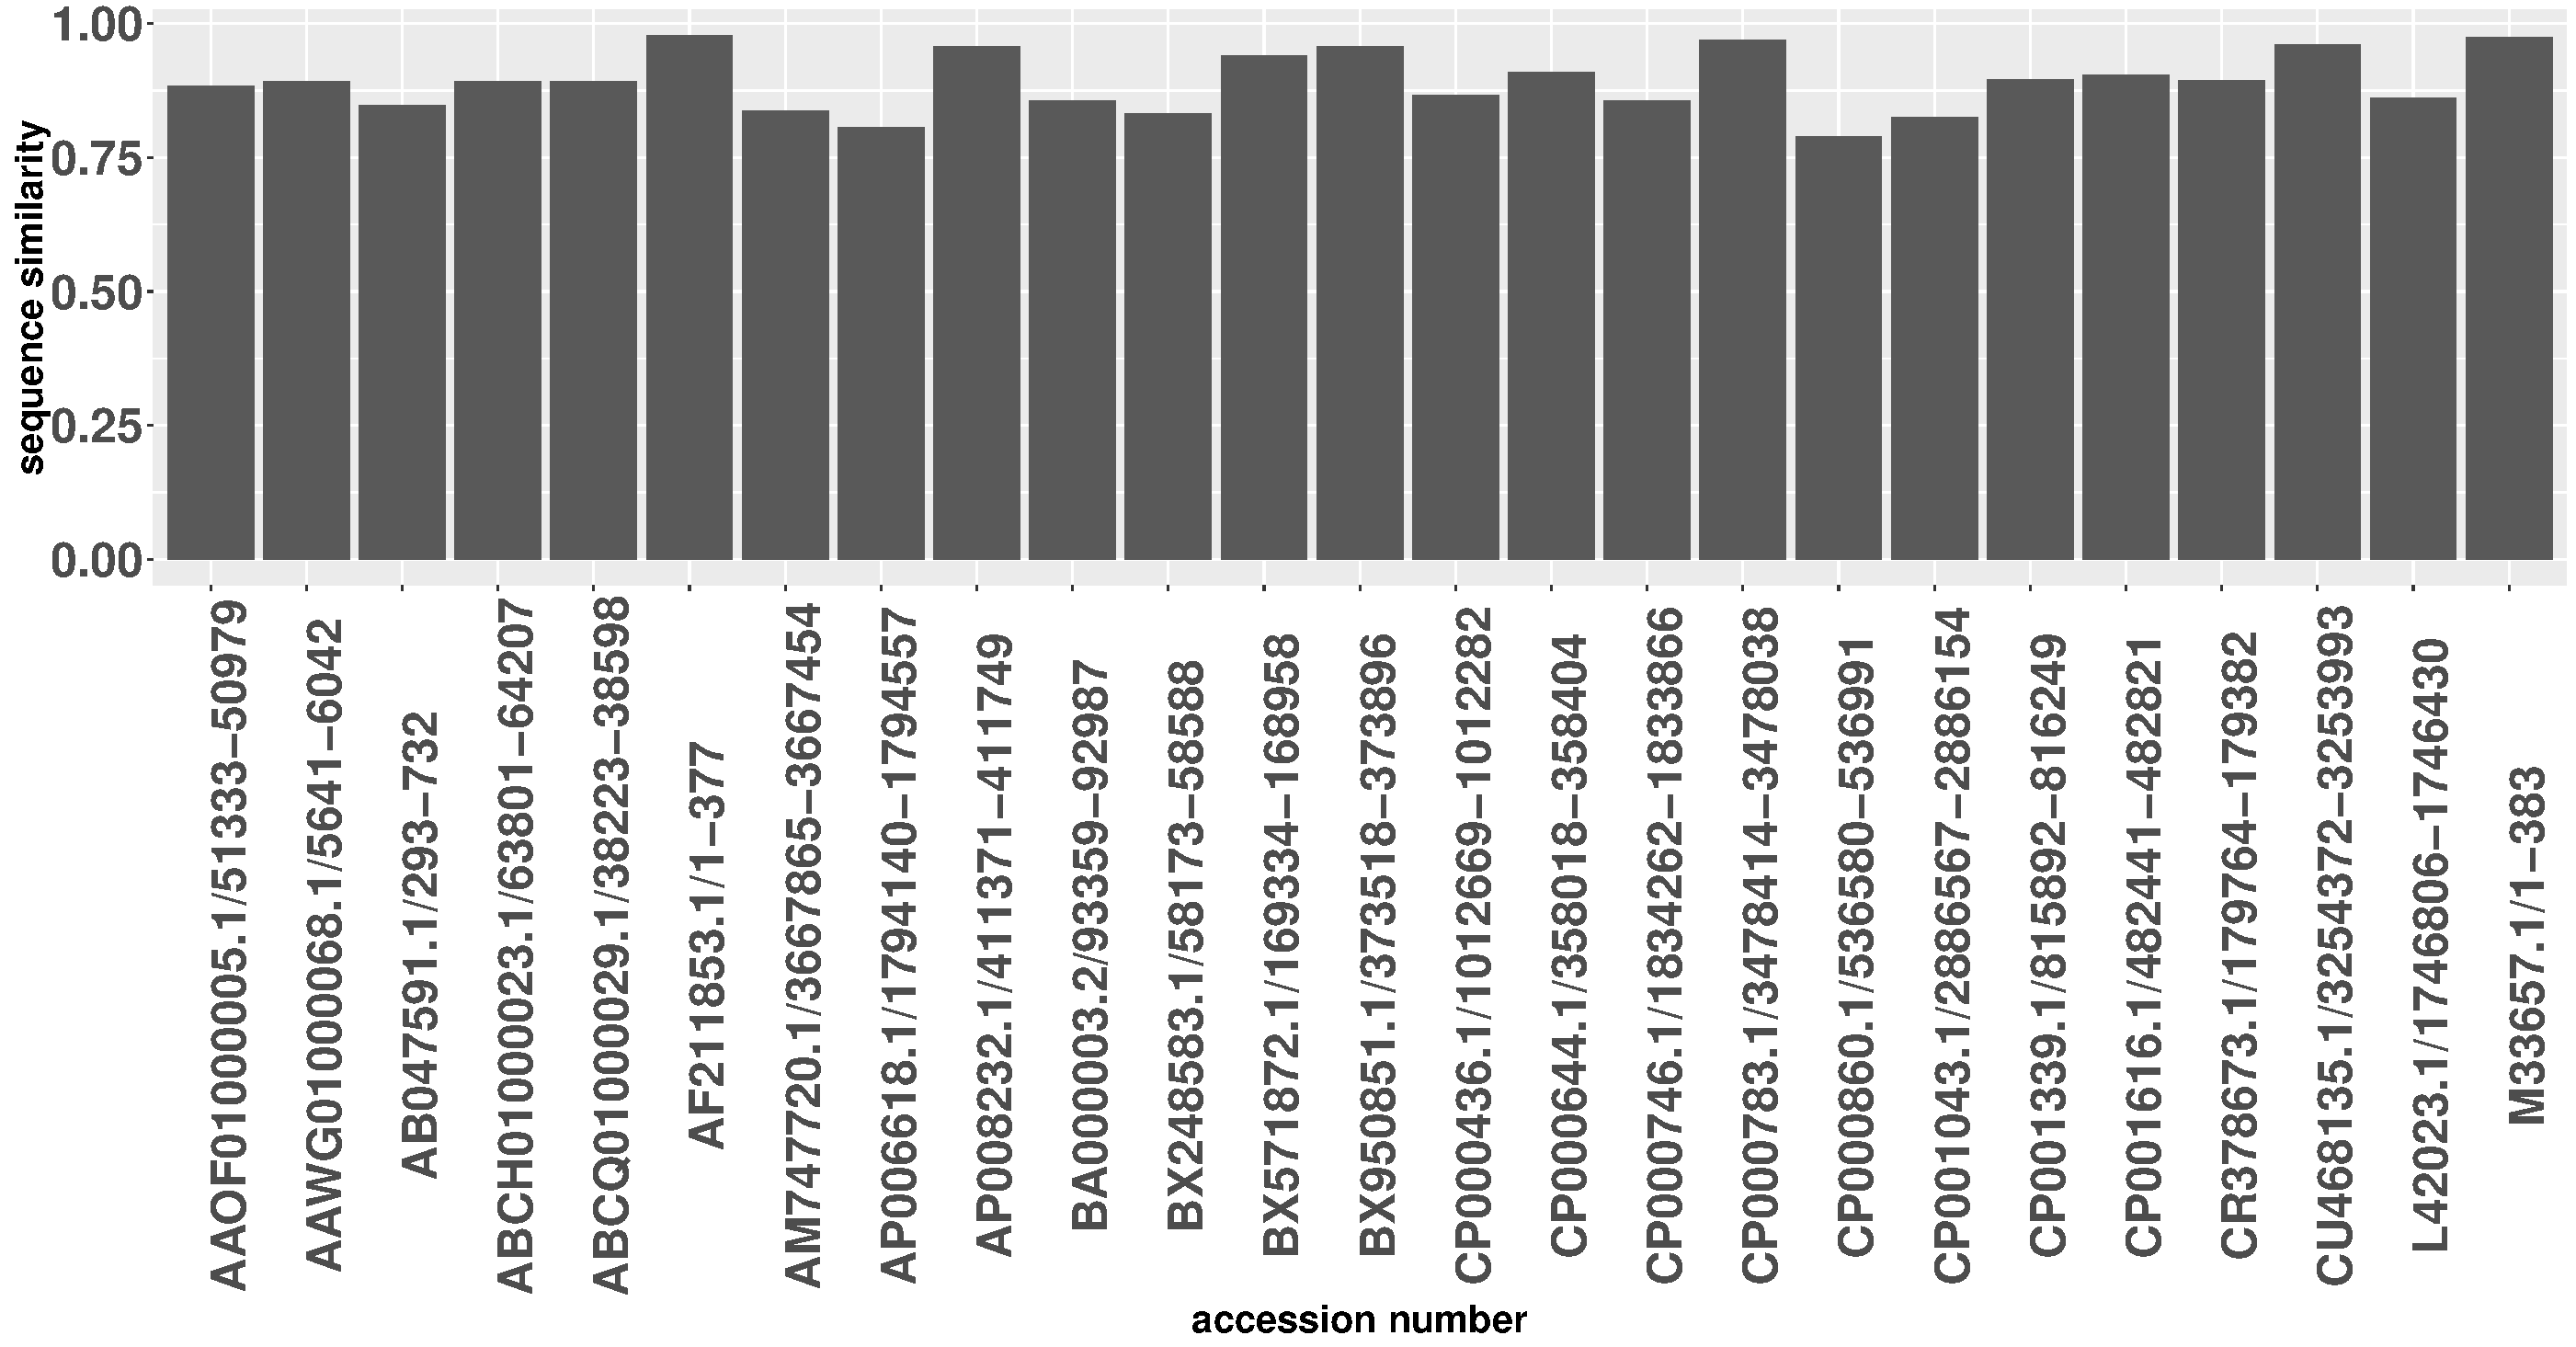
\includegraphics[width=0.5\textwidth]{./pictures/sequenceSimilarity/RNaseP.pdf} &
 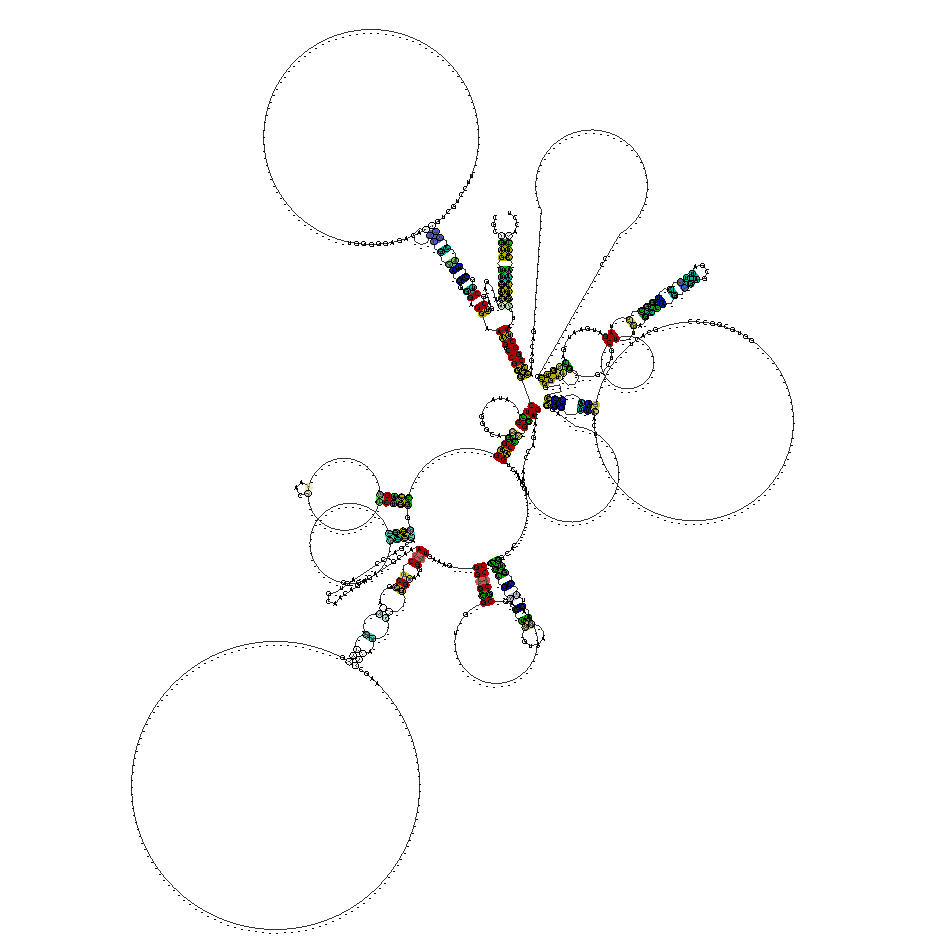
\includegraphics[width=0.4\textwidth]{./pictures/consensusStructure/RNaseP.pdf}\\
\end{tabular}
\caption{{\bf Sequence similarity  to the reference sequences and consensus structure of \texttt{SRP}, \texttt{trpL} and \texttt{RNaseP} family members.} 
  (a) \texttt{SRP} RNA: average sequence similarity ($\bar{S}$) = 0.682, ref. seq. = X01074.1/170-275. 
  			   SCI : 0.8379													 
  (b) trpL:  $\bar{S}$ = 0.658, ref. seq. = AE005174.2/2263095-2263188. 
			 SCI : 0.5312	 					 						   
  (c) RNaseP: $\bar{S}$ = 0.891, ref. seq. = CP001509.3/3136785-3136410
			  SCI : 	0.7854	 				}
\label{fig:sequence_similarity}
\end{figure}
      

\FloatBarrier
		
%\begin{table}[ht]
%\begin{tabular}{l|l|l|l}  
%{alignment} & {SCI} & {with ribosum scoring} & {sequence similarity}\\  
%\hline
%RF00169 & 0.8379 & 1.4266 & 0.682\\ 
%RF00513 & 0.5312 & 1.2229 & 0.658\\
%RF00010 & 0.7854 & 1.3666 & 0.891\\
% \end{tabular} 
%\caption{Comparison of SCI and sequence similarity. Dangle option 2 was used to calculate SCI.}
%\label{fig:compare_SCI_sequence_similarity}
%\end{table}





\FloatBarrier
		

\section{base-pair diversity}
  
Base-pair diversity is used to determine how many different base-pairs a
sequence forms during and after co-transcriptional folding, and how many
could have been formed theoretically.
I calculated the bp diversity for all of the three 
reference sequences and over all possible \texttt{Kinwalker} parameter
combinations in both time-independent (eq.~\ref{eq:base-pair diversity})
and dependent (eq.~\ref{eq:base-pair diversity time depended}) manner
 and compared the resulting scores with each other. 

As expected, the time-dependent base-pair diversity for every RNA family is in general lower and more constant over all \texttt{Kinwalker} parameter than the time-independent bp-diversity (fig.~\ref{fig:base-pair diversity}).

For \texttt{SRP} reference sequence,  time-dependent diversity remains constant over
all parameters and only shows a small drop at transcription rates of 270 to 300
nt/s (\texttt{findpath}/dangle 2) and 20 nt/s (\texttt{Morgan$-$Higgs}/dangle
$0$). The time-independent bp diversity gives similar results for these
transcription rates. However, here the individual parameter combinations
influence overall bp diversity much more than for the time-dependent scores
(fig.~\ref{fig:base-pair diversity} a).
In the case of \texttt{trpL}, base-pair diversities are more robust regarding parameter
combinations (fig.~\ref{fig:base-pair diversity} b).
%stays constant over all parameters; small time-dependent diversity decrease at transcription rates ranging from 60 to 90 nt/s with findpath/dangle 2.

\texttt{RNaseP} shows a drastic increases in base-pair diversity when calculated
time-independent at transcription rates ranging from 230 to 430 nt/s
(\texttt{Morgan$-$Higgs}/dangle 2) as well as from 50 to 500 nt/s
(\texttt{findpath}/dangle 2). None of these increases appear with the time-dependent
diversity (fig.~\ref{fig:base-pair diversity} c).


%To determine how \texttt{Kinwalker} parameters influence base-pair
%diversity during folding of RNAs, 
% If every formed base-pair would exist for the whole folding time, scoring with time-factor would result the same result as without time-factor. This implicates, that if calculated with a time scoring function (like equation:~\ref{eq:base-pair diversity time depended}), the base-pair diversity score is generally lower (as shown in figure:~\ref{fig:base-pair diversity SRP},~\ref{fig:base-pair diversity TRP} and~\ref{fig:base-pair diversity RNAseP}).

 

\begin{figure}[ht]
\centering
\begin{tabular}{c|c}
time-independent & time-dependent\\
\hline
(a) \texttt{SRP} \\
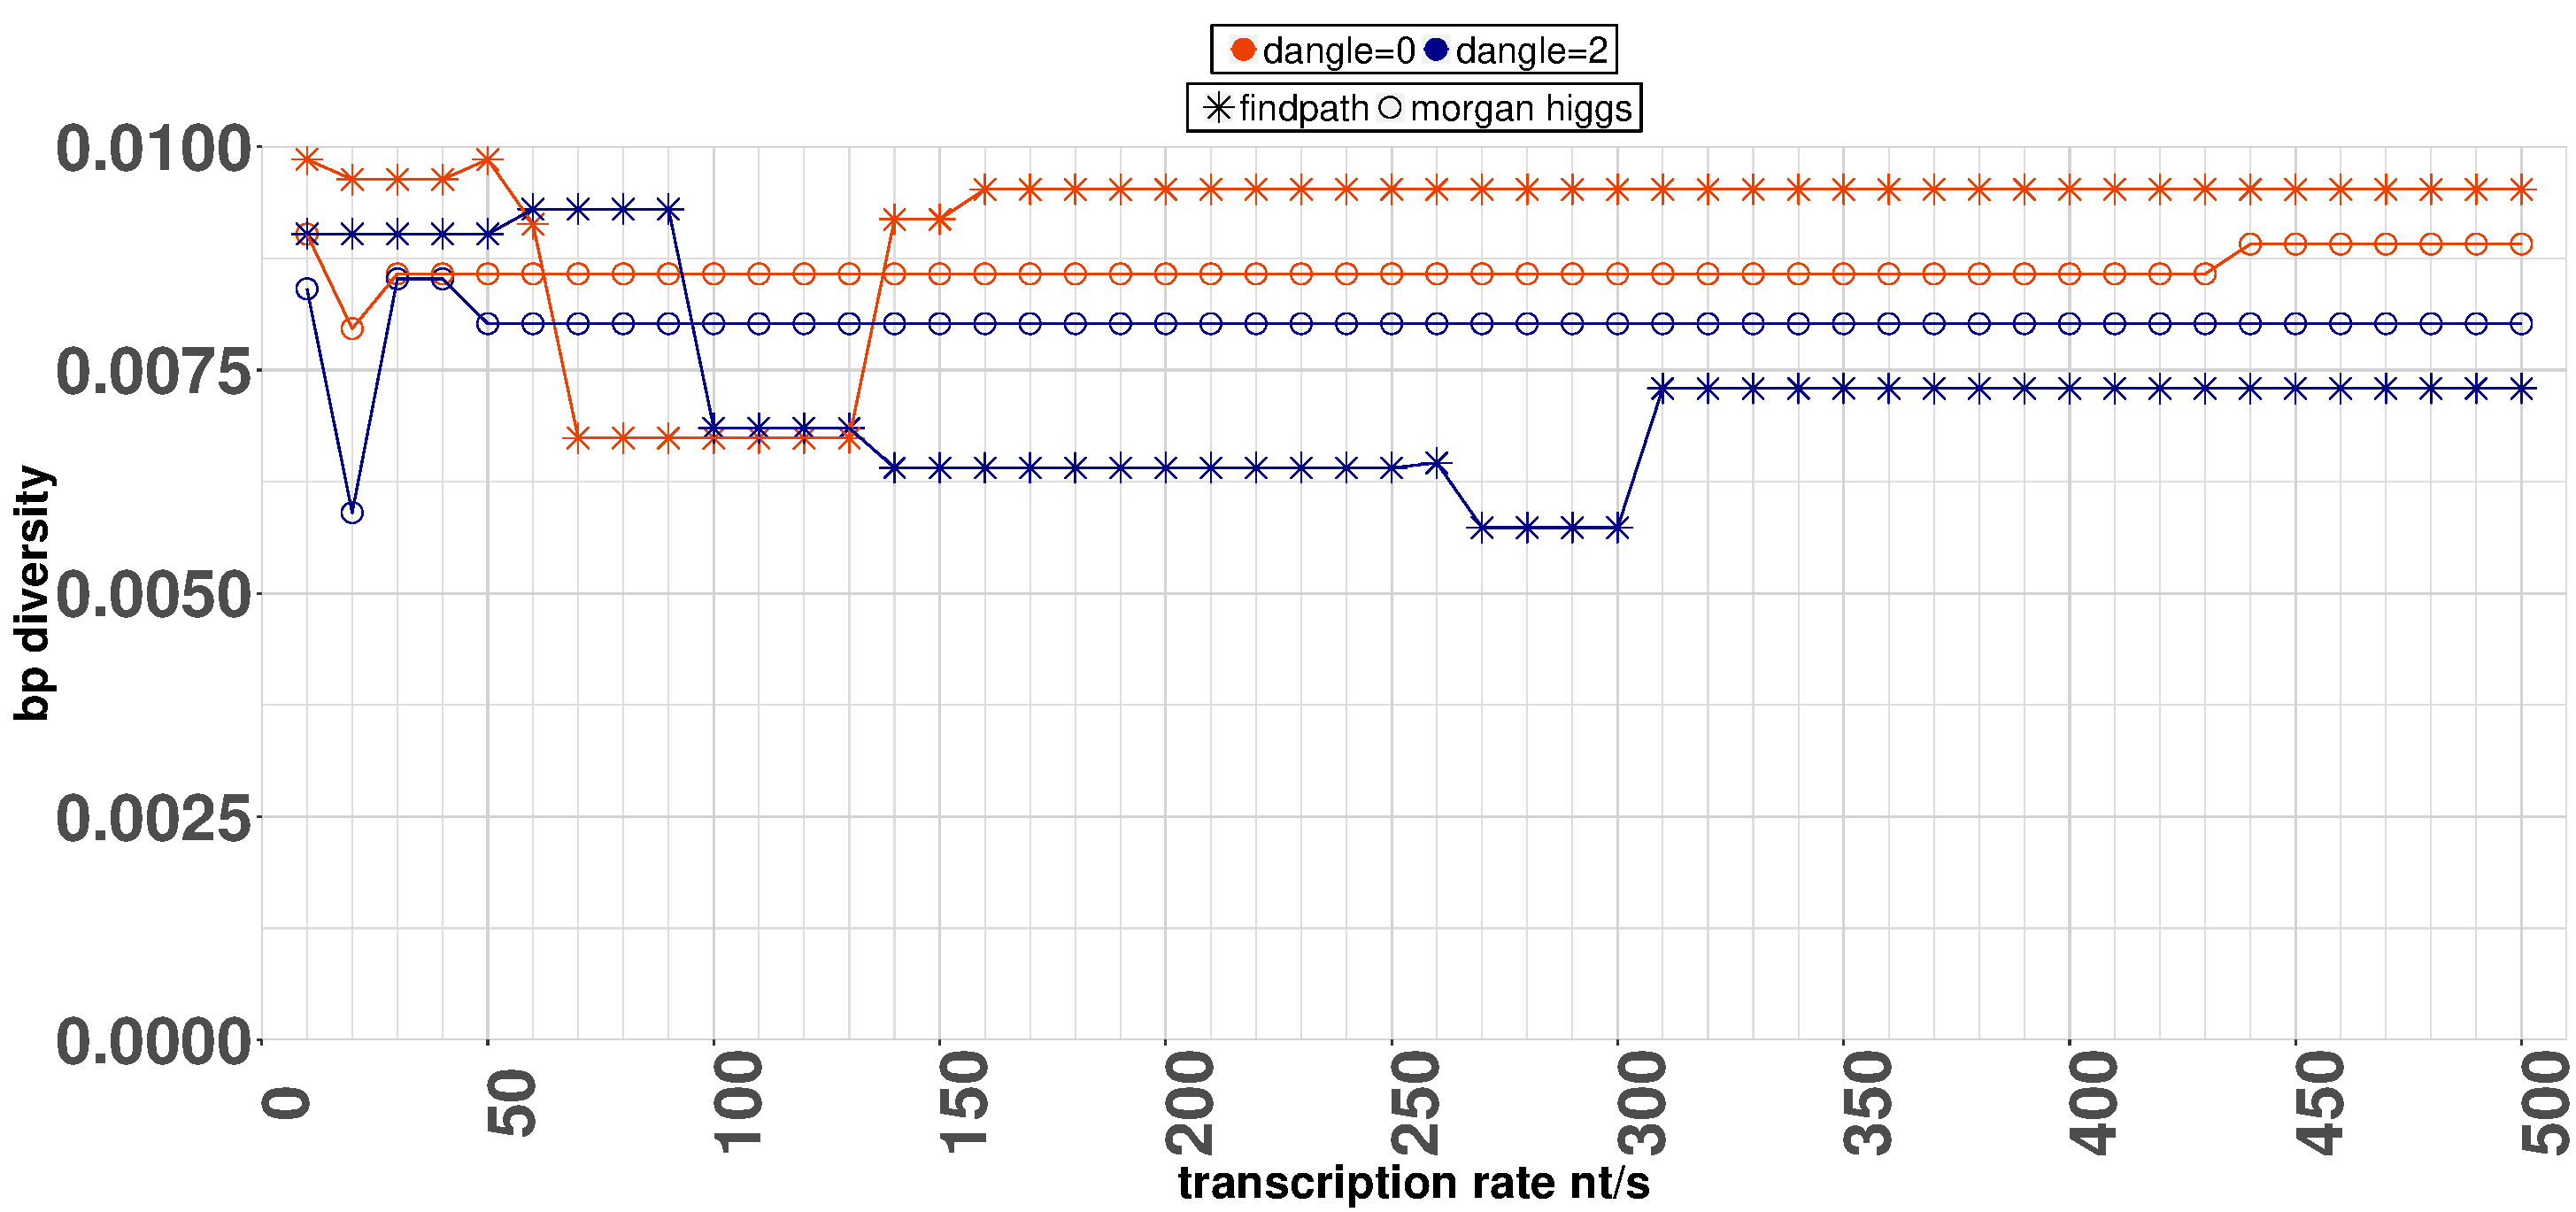
\includegraphics[width=0.5\textwidth]{./pictures/basePairDiversity/WithoutTime/SRP-WithoutTime.pdf} &
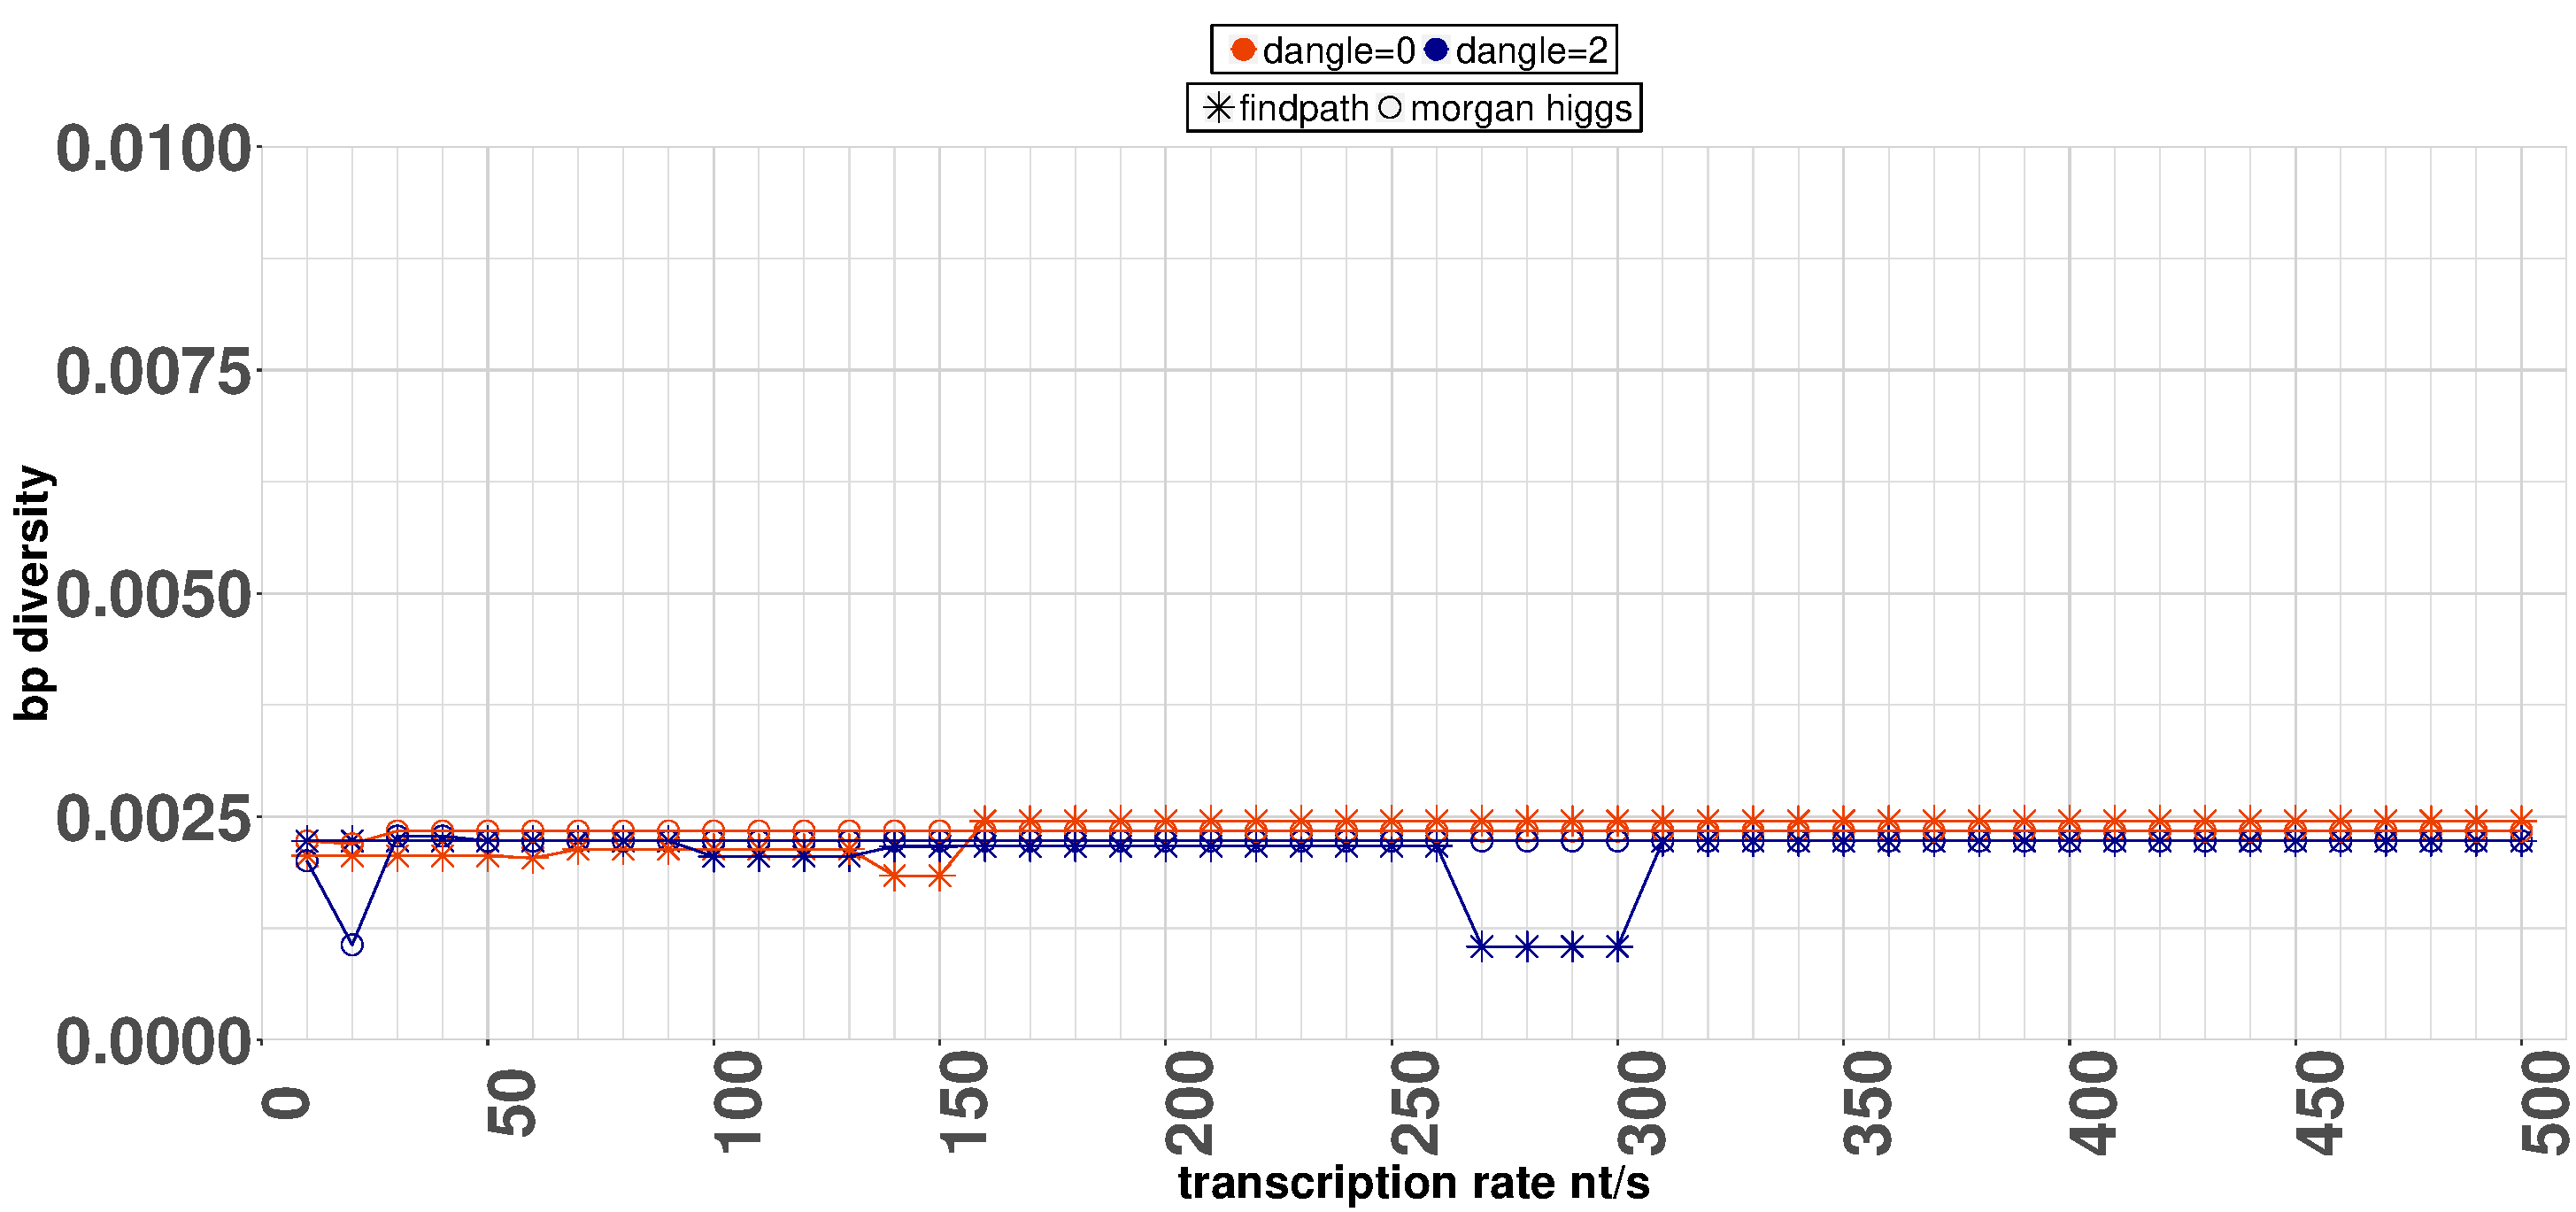
\includegraphics[width=0.5\textwidth]{./pictures/basePairDiversity/TimeDepended/SRPWithTime.pdf}\\
\hline
(b) \texttt{trpL} \\
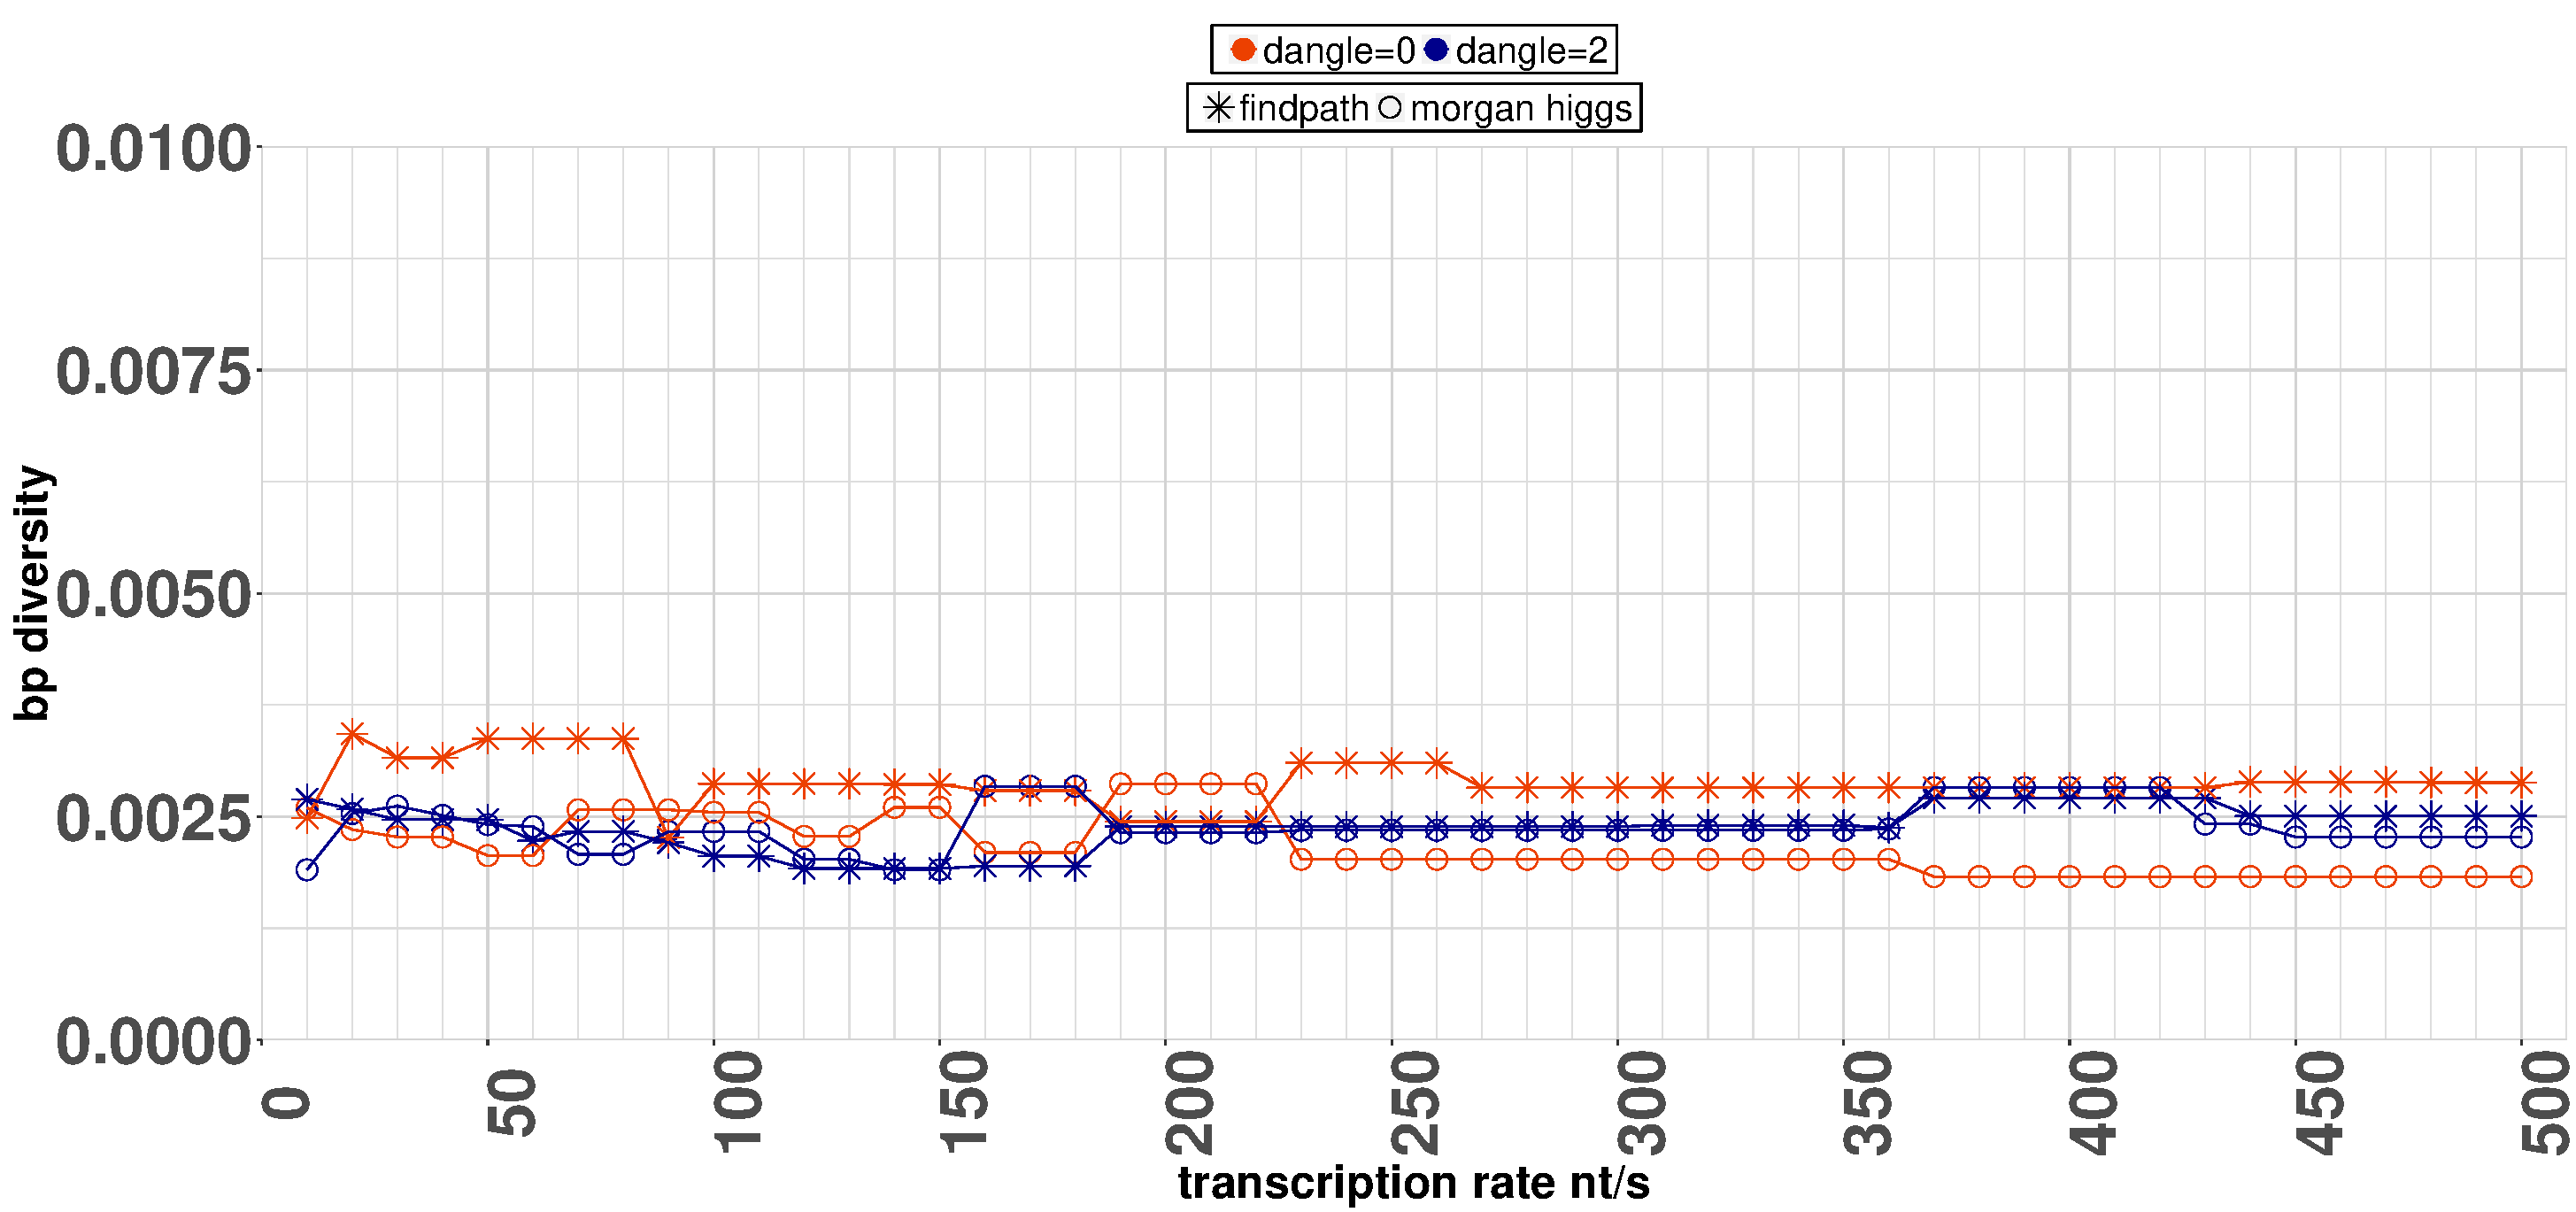
\includegraphics[width=0.5\textwidth]{./pictures/basePairDiversity/WithoutTime/TRP-WithoutTime.pdf}&
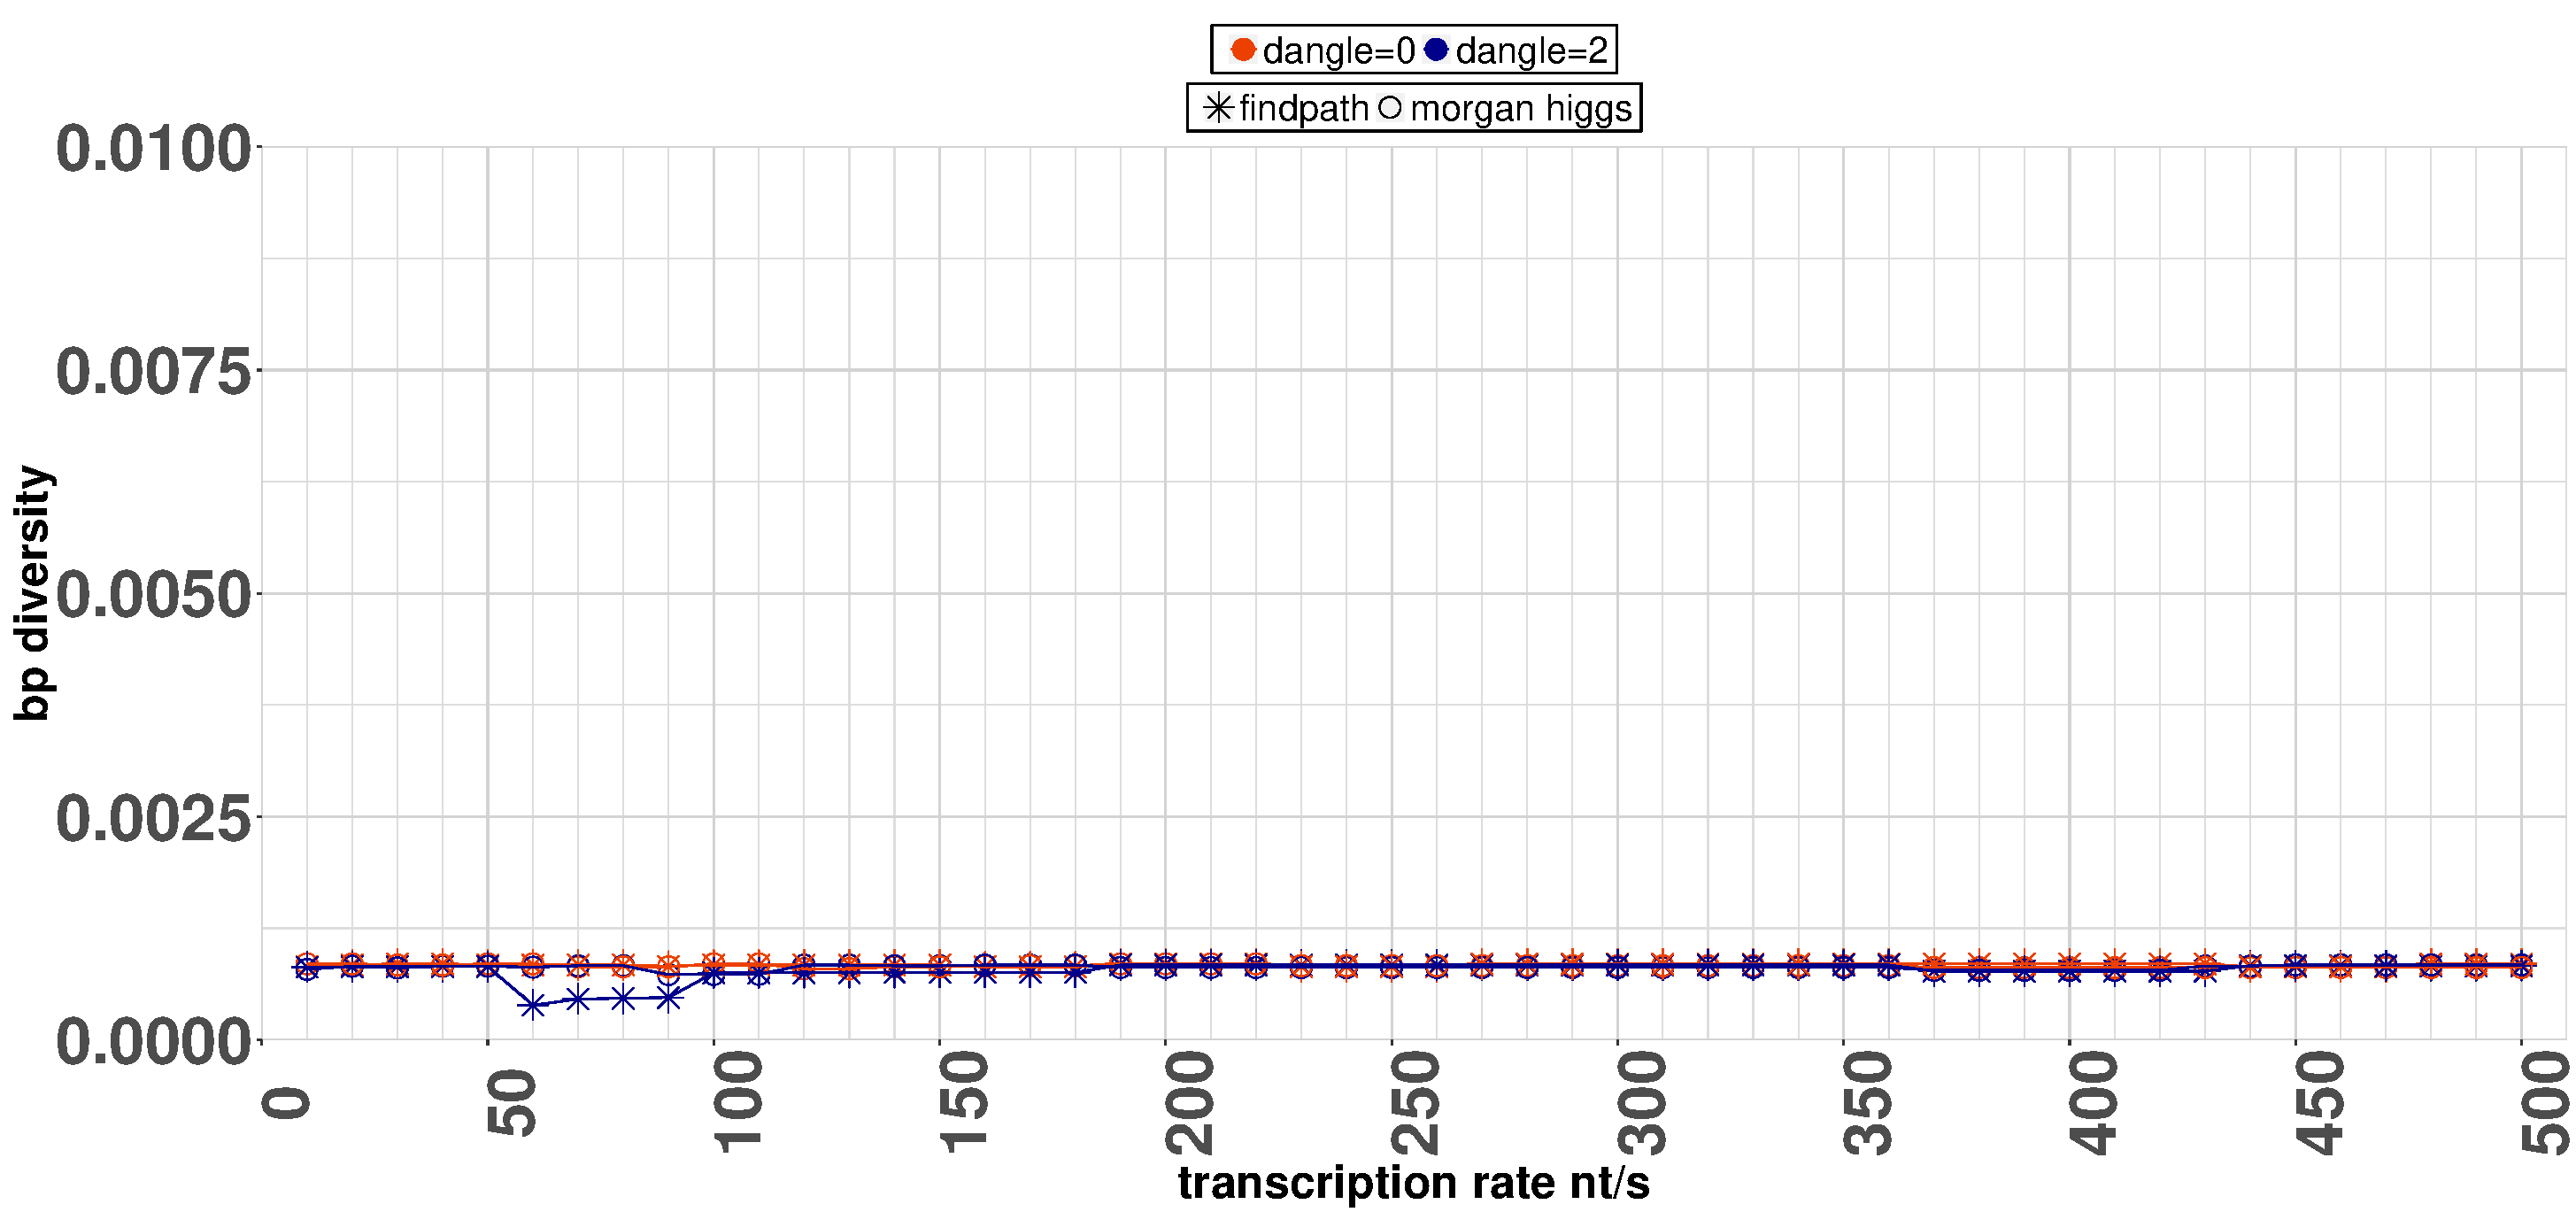
\includegraphics[width=0.5\textwidth]{./pictures/basePairDiversity/TimeDepended/TRPWithTime.pdf}\\
\hline
(c) \texttt{RNaseP} \\
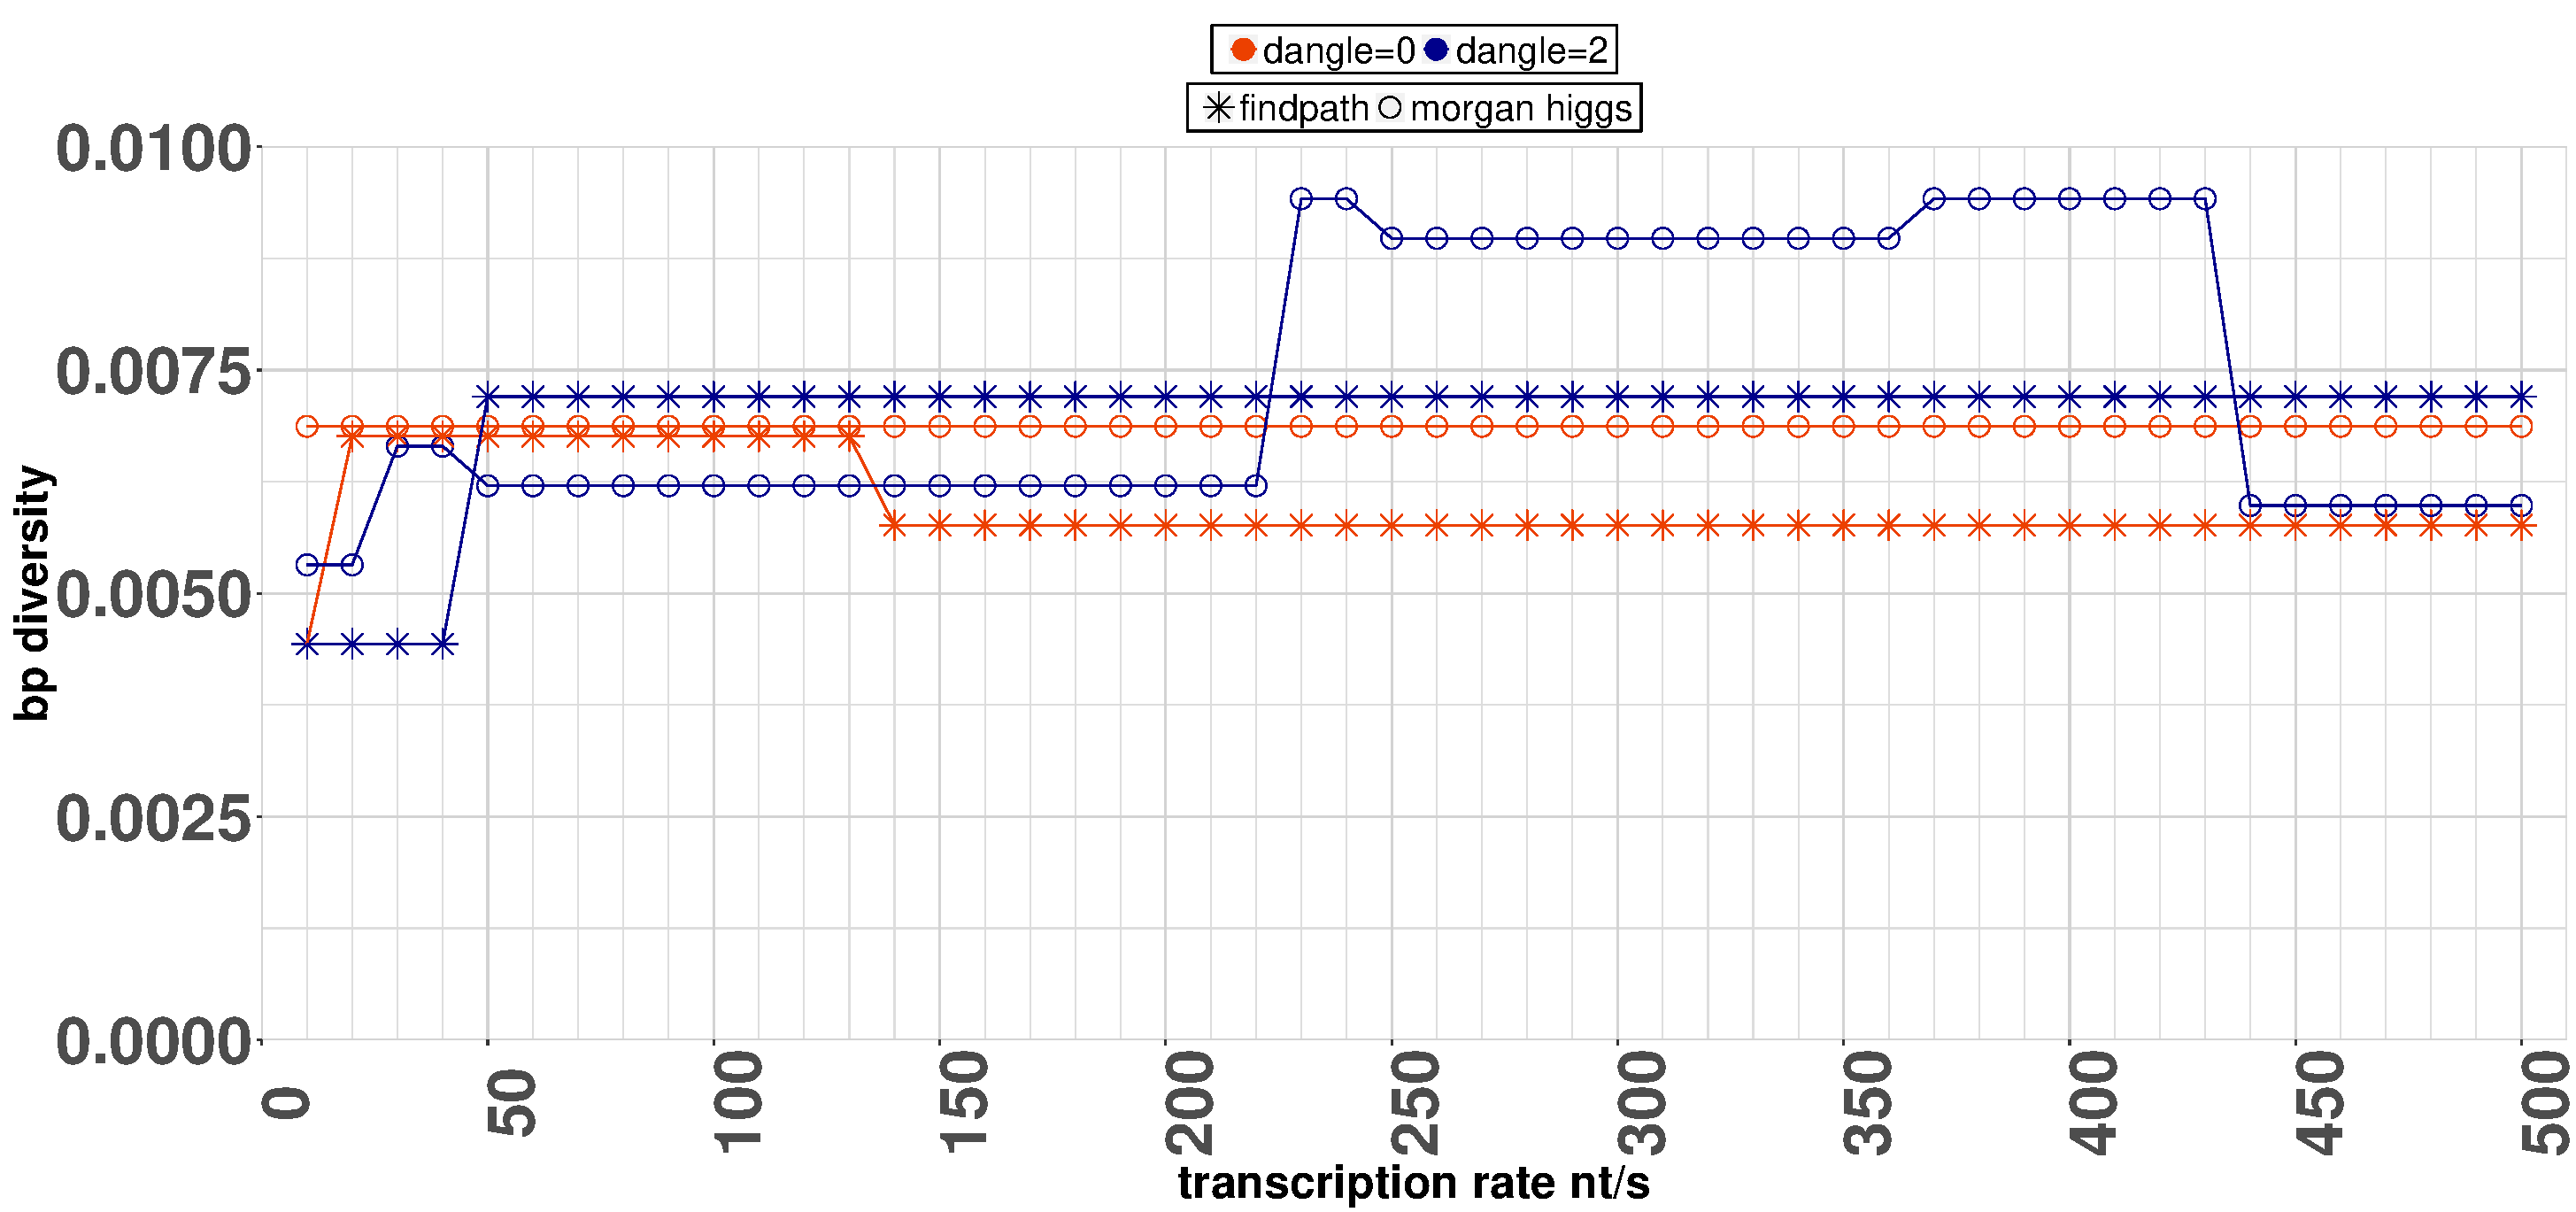
\includegraphics[width=0.5\textwidth]{./pictures/basePairDiversity/WithoutTime/RNAseP-WithoutTime.pdf}&
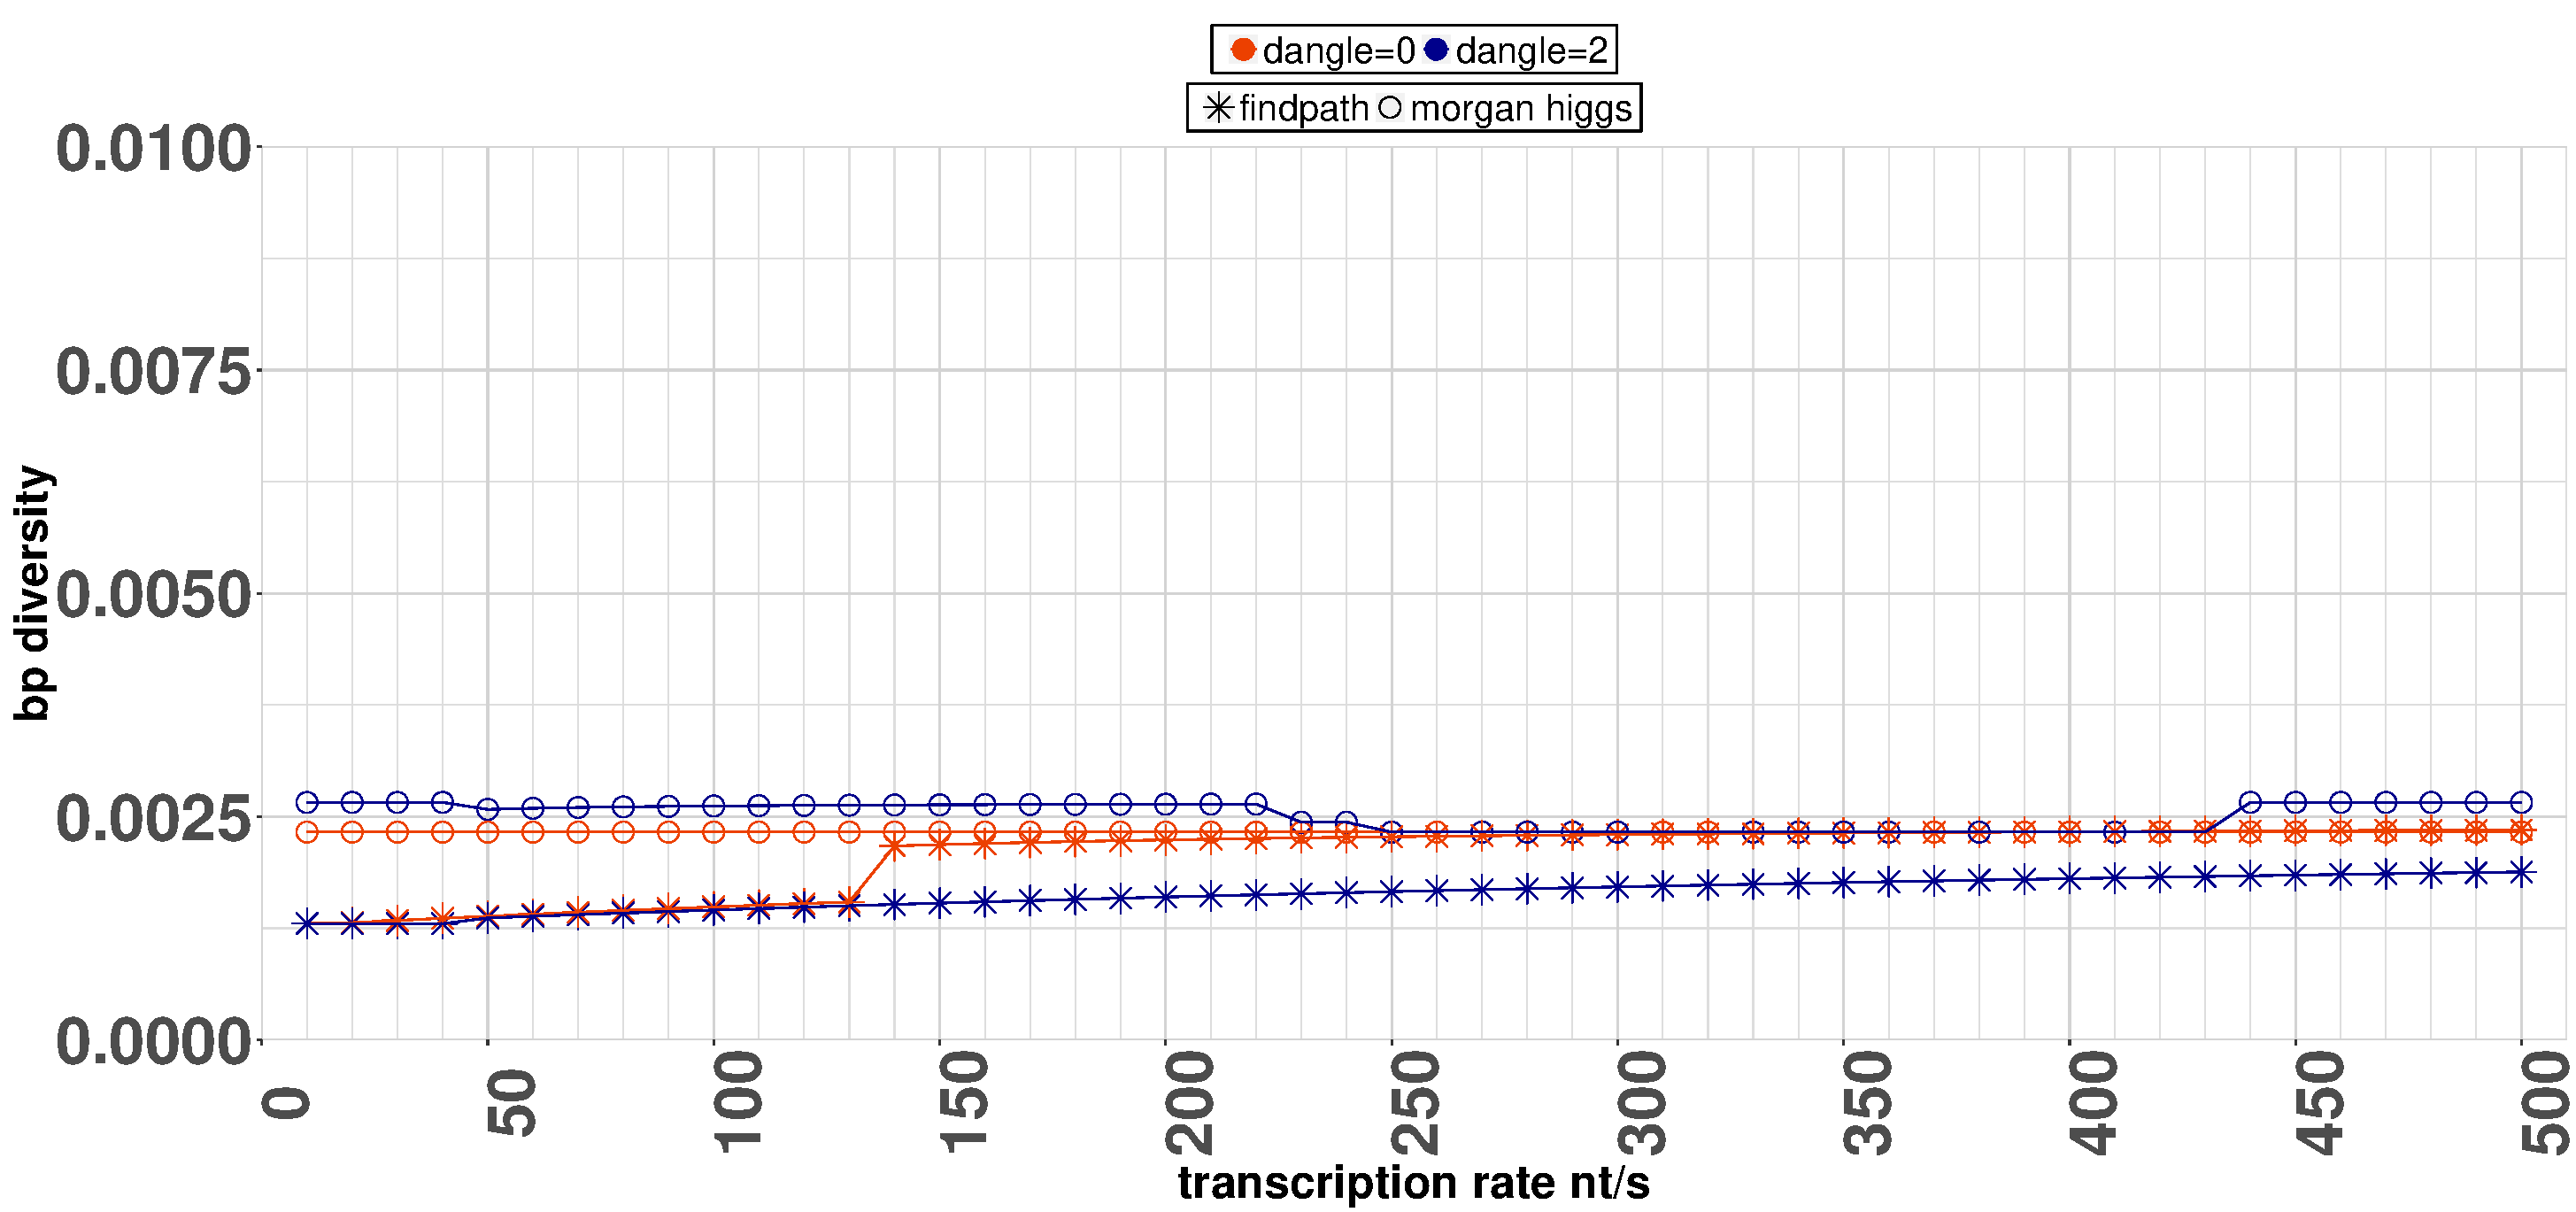
\includegraphics[width=0.5\textwidth]{./pictures/basePairDiversity/TimeDepended/RNAsePWithTime.pdf}\\

\end{tabular}
\caption{{\bf bp diversity for references sequences}. 
(a) Base-pair diversity for \texttt{SRP} reference sequence. Constant time-dependent diversity over all parameters. Diversity drops for both scores at transcription rates of 270 to 300 nt/s if \texttt{findpath}/dangle 2 was used as well as with transcription rate of 20 nt/s and \texttt{Morgan$-$Higgs}/dangle $0$. 
(b) Base-pair diversity for \texttt{trpL} reference sequence. Diversity stays constant over all parameters; small time-dependent diversity decrease at transcription rates ranging from 60 to 90 nt/s with \texttt{findpath}/dangle 2.
(c) Base-pair diversity for \texttt{RNaseP} reference sequence. Constant time-dependent diversity over all parameters. Time-independent diversity increase happens with transcription rates ranging from 230 to 430 nt/s with \texttt{Morgan$-$Higgs}/dangle 2 as well as with transcription rates ranging from 50 to 500 nt/s if \texttt{findpath}/dangle 2 was used. None of these increases appear with the time-dependent diversity.
}
\label{fig:base-pair diversity}
\end{figure}
		
For comparison of base-pair diversity of sequences within their RNA family,
each time-dependent base-pair diversity was plotted for each sequence
(fig.~\ref{fig:base-pair diversity alignments}).
Here we selected the best parameter combination (\texttt{findpath} and
dangle option 2), because these parameters provide in general a more
realistic model for \textit{in silico} RNA folding simulations, reflected
by in generally lower base-pair diversities (fig.~\ref{fig:base-pair diversity}).
%For data simplification only time-dependent base-pair diversity,
%\texttt{findpath} algorithm, and  were used for this comparison. These
%specific parameter set was chosen, because "\texttt{findpath} and dangle
%2" are theoretically\footnote{specified by my working group} the best
%approach for \textit{in silico} RNA folding prediction.
Overall, base-pair diversity is more diverse at lower transcription rates and becomes more constant with increasing transcription rates. 	

In the case of \texttt{SRP} RNA, 
more changes in base-pair diversity are observed at transcription rates below 140
nt/s. A noticeable drop in base-pair diversity is observed at transcription rates ranging from 270 to
300 nt/s for five sequences (fig.~\ref{fig:base-pair diversity alignments} a).
Members of the \texttt{trpL} family show rather constant diversity over all \texttt{Kinwalker} parameters (fig.~\ref{fig:base-pair diversity alignments} b).
Like \texttt{SRP} RNA, \texttt{RNaseP} family members have 
more changes in base-pair diversity at lower transcription rate ($\le$ 120 nt/s), but rather constant base-pair diversity at higher transcription rates (fig.~\ref{fig:base-pair diversity alignments} c).


\begin{figure}[ht] 
\centering
\begin{tabular}{c}
(a) \texttt{SRP} \\
 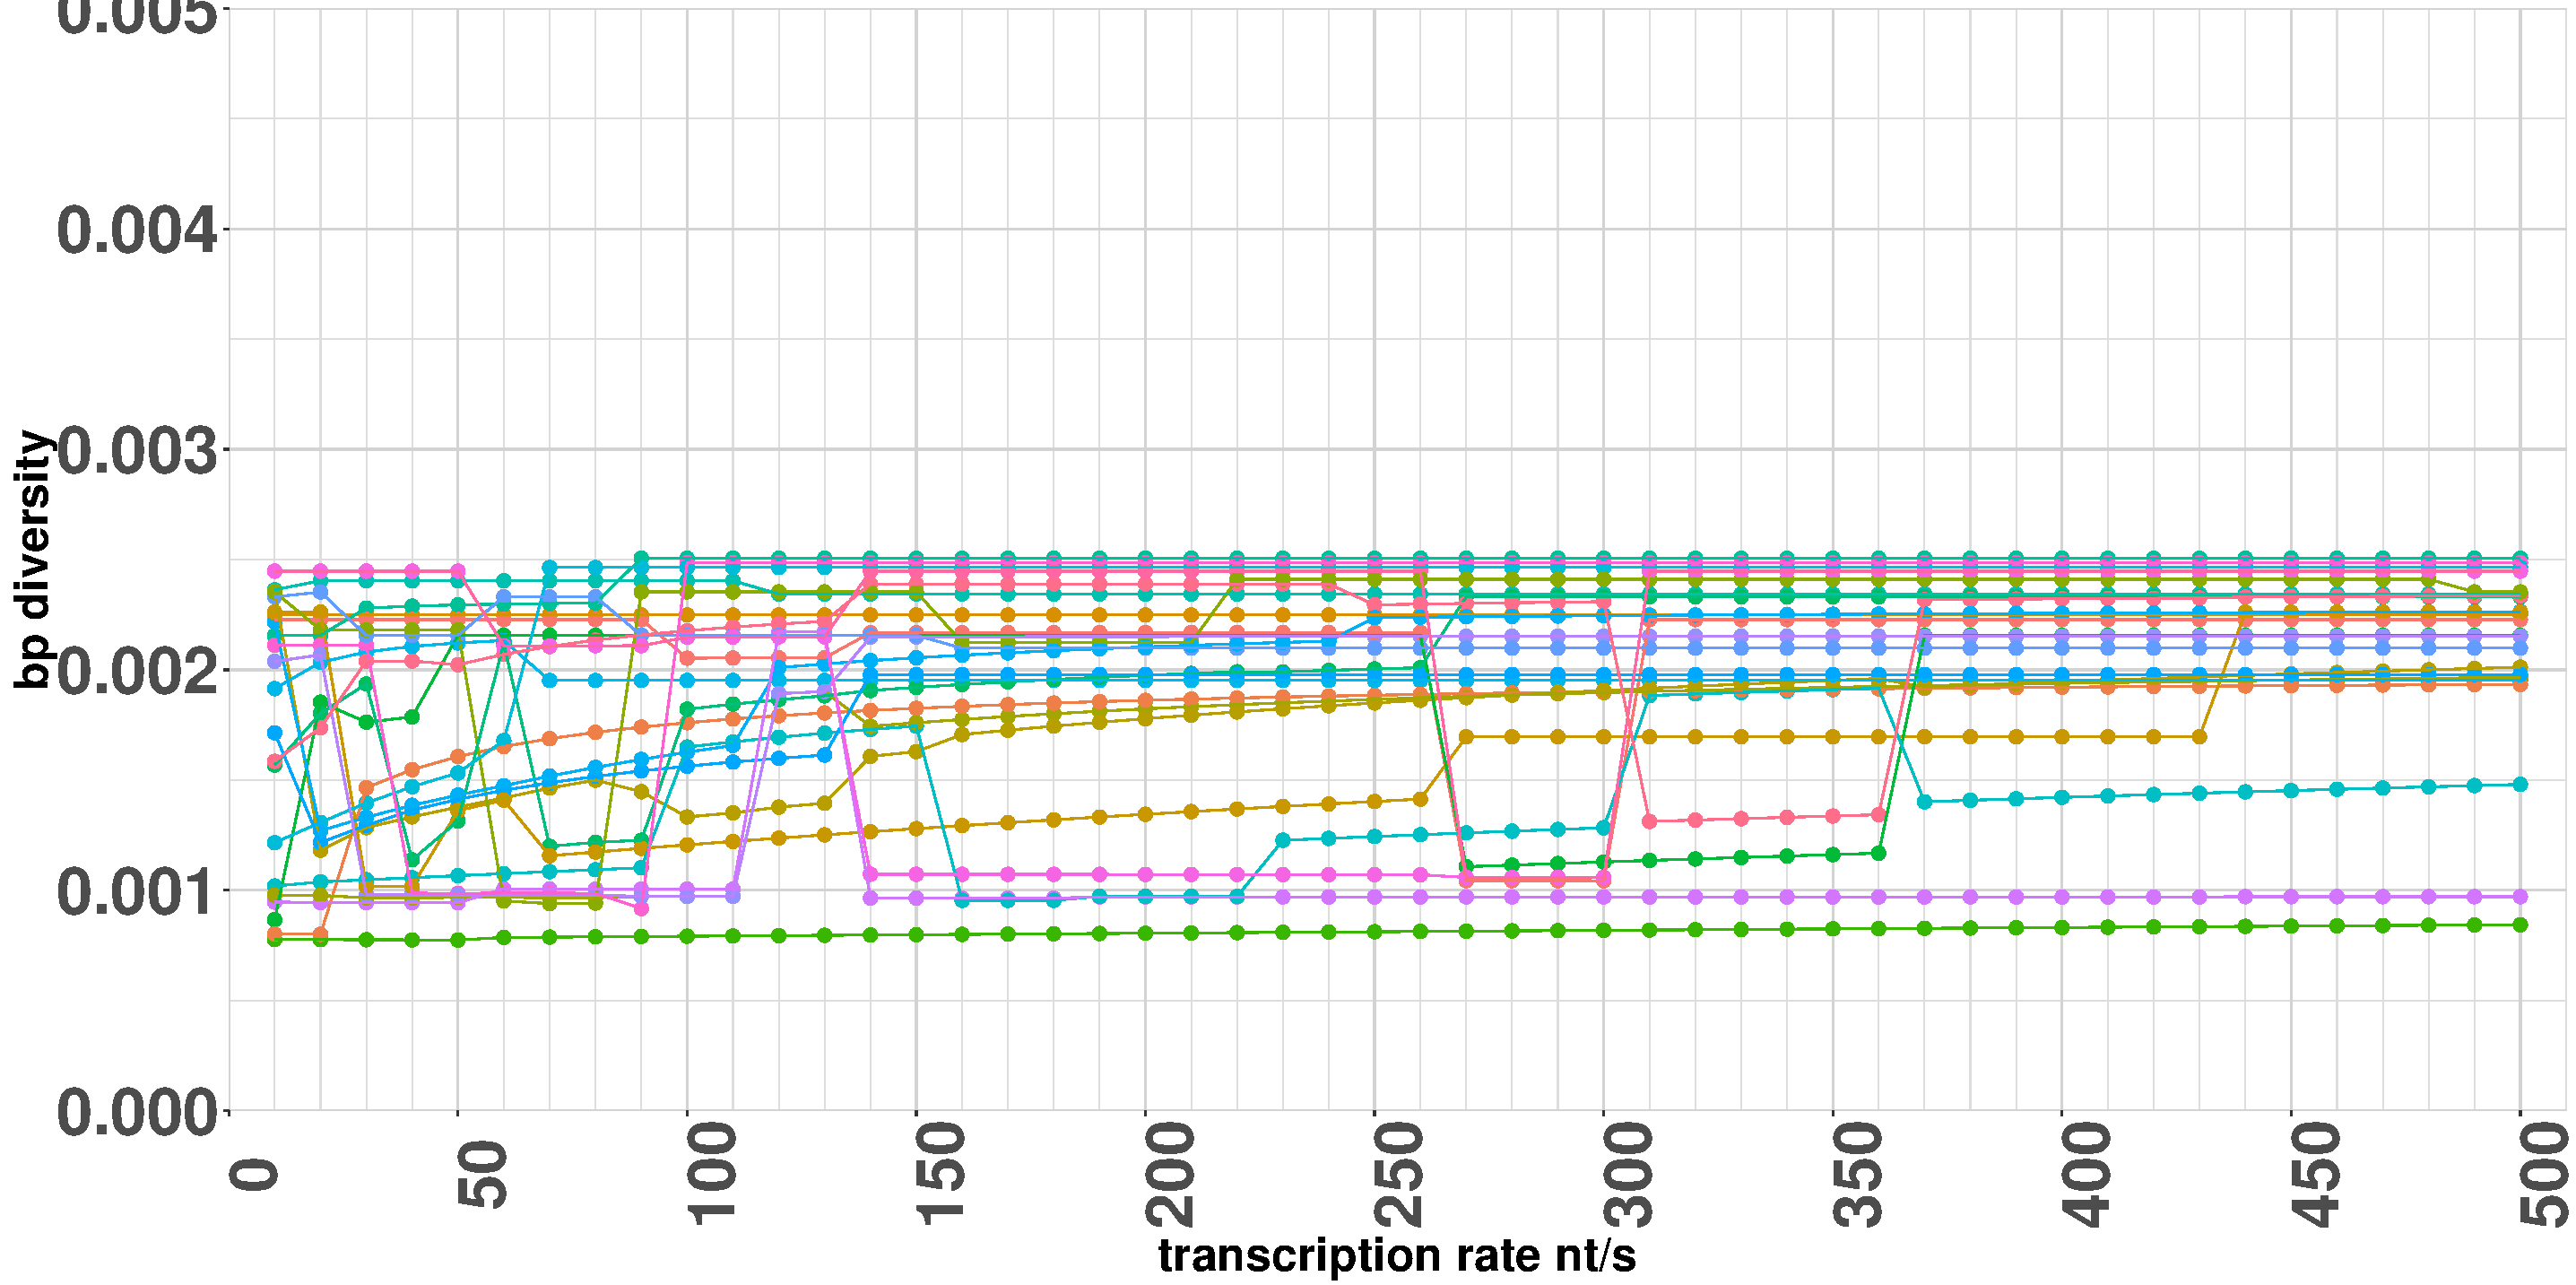
\includegraphics[width=0.85\textwidth]{./pictures/basePairDiversity/TimeDepended/forAlignment/RF00169.pdf} \\
\hline
(b) \texttt{trpL} \\
 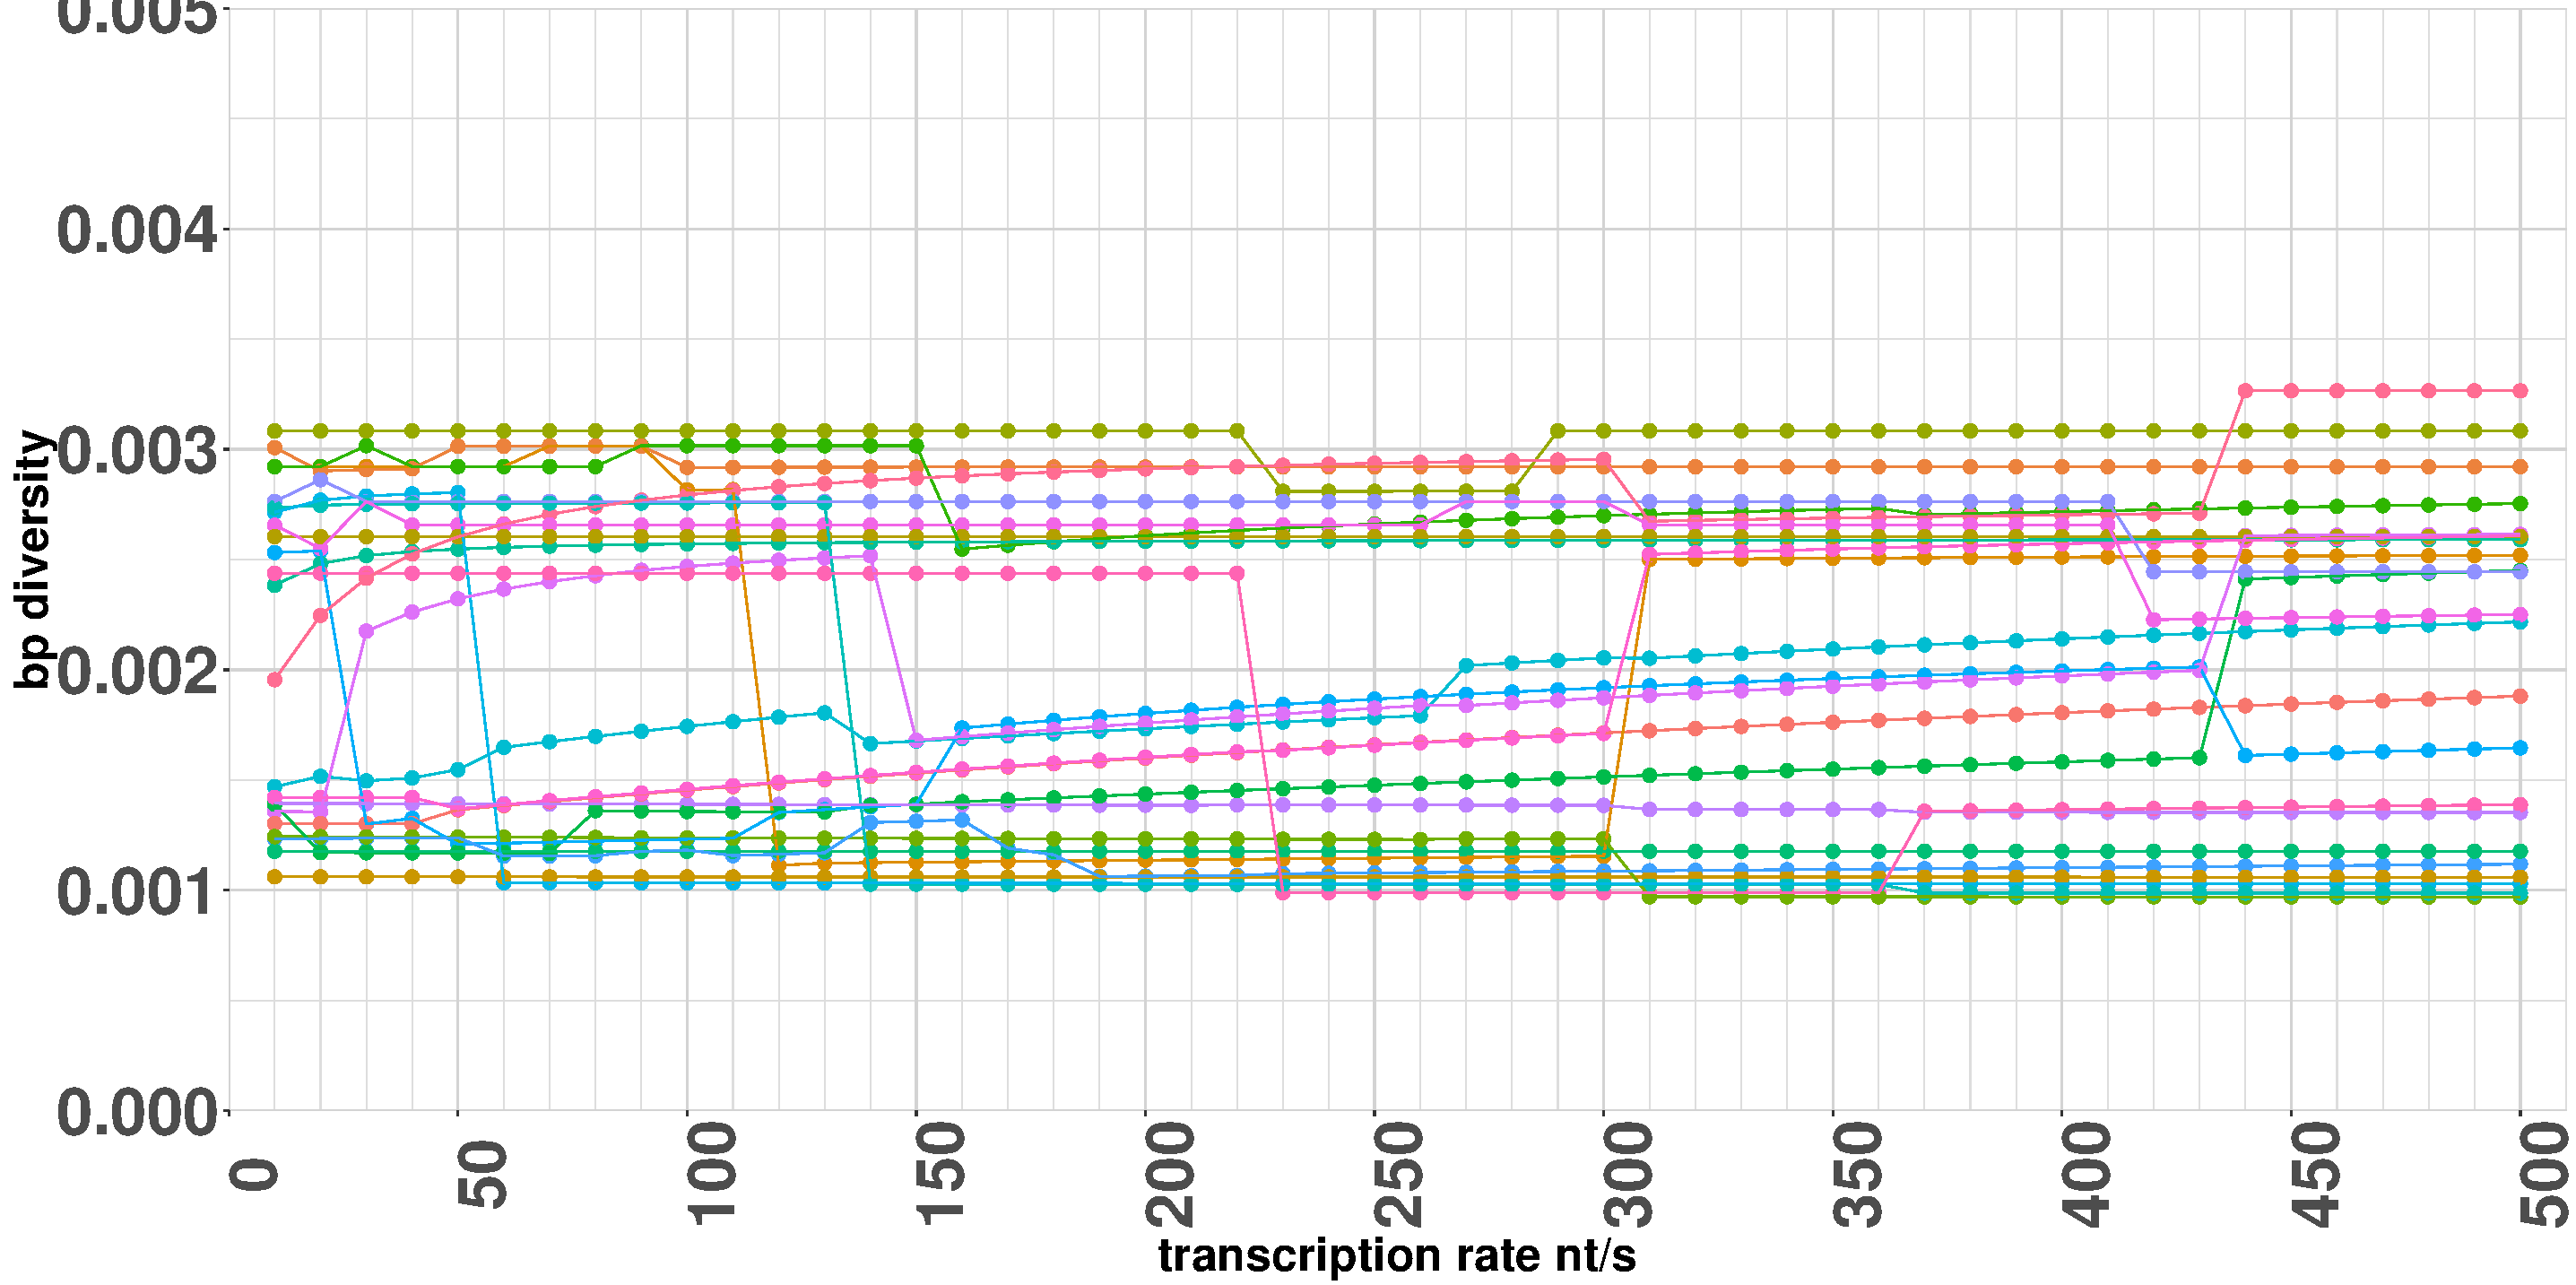
\includegraphics[width=0.85\textwidth]{./pictures/basePairDiversity/TimeDepended/forAlignment/RF00513.pdf} \\
\hline
(c) \texttt{RNaseP} \\
 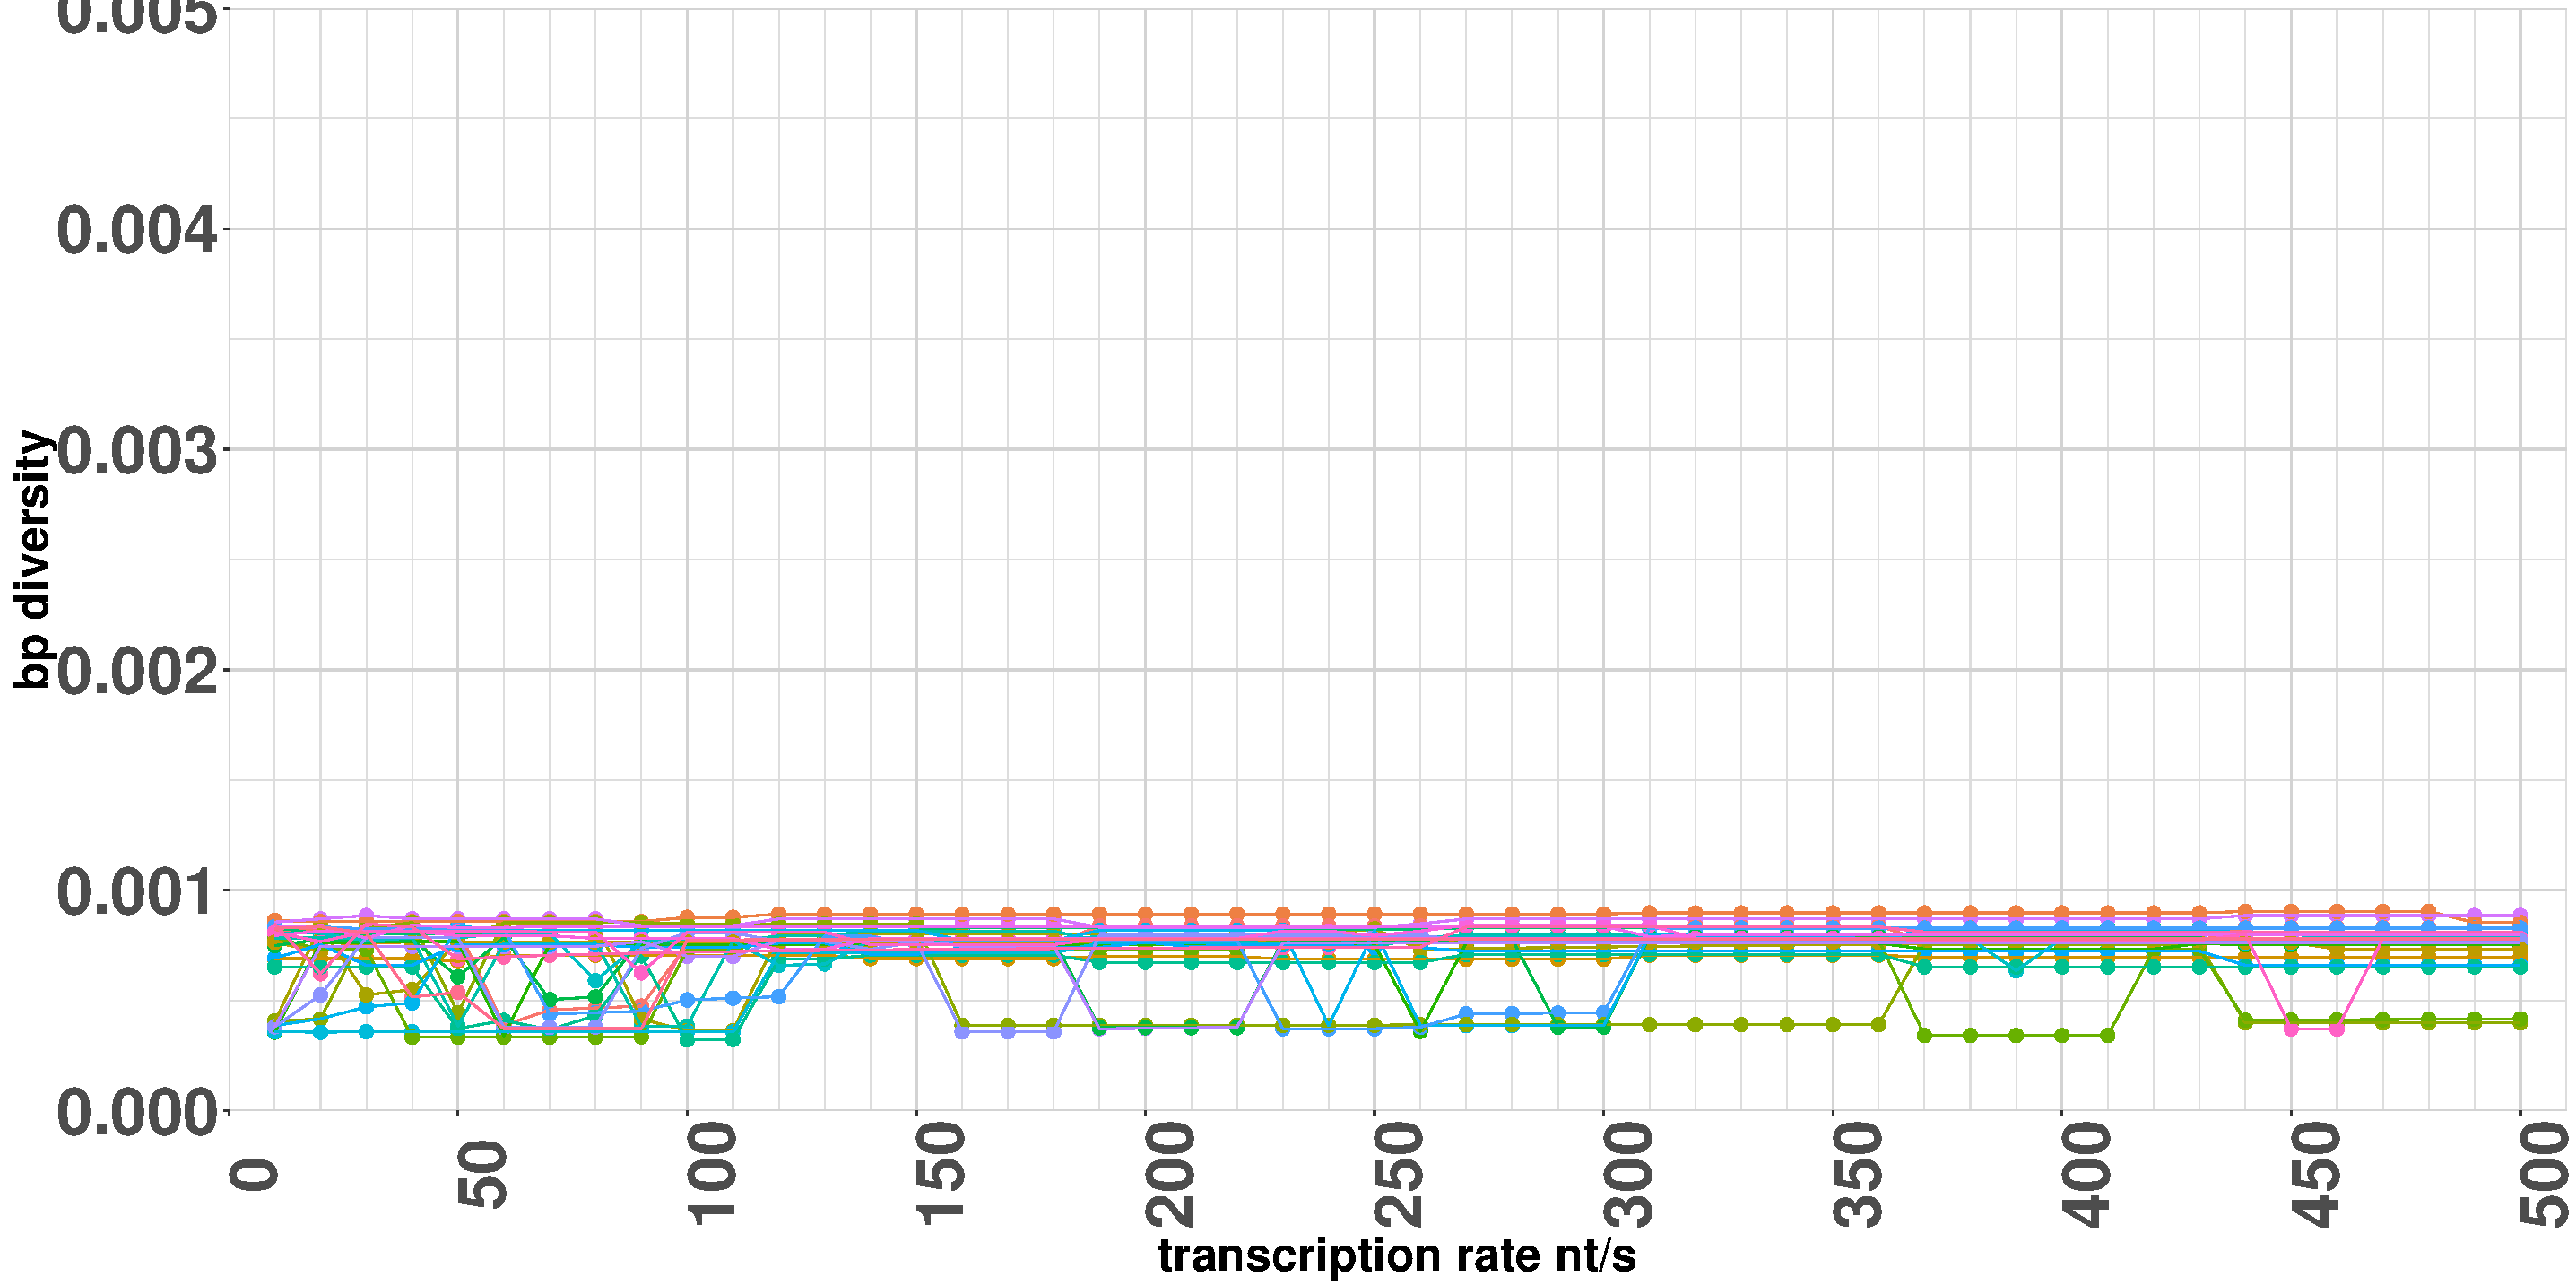
\includegraphics[width=0.85\textwidth]{./pictures/basePairDiversity/TimeDepended/forAlignment/RF00010.pdf} \\
\end{tabular}				

\caption{ {\bf base-pair diversity for RNA families}.
\texttt{Kinwalker} parameter-set used : \texttt{findpath}, dangle option 2 and transcription rates ranging from 0 to 500 nt/s.
(a) base-pair diversity for \texttt{SRP} family. 
More changes in diversity if transcription rate below 140 nt/s were used. Noticeable diversity drop at transcription rates ranging from 270 to 300 nt/s for five sequences.
(b) base-pair diversity for \texttt{trpL} family. 
Rather constant diversity over all \texttt{Kinwalker} parameters.
(c) base-pair diversity for \texttt{RNaseP} family. 
More changes in diversity if transcription rate below 120 nt/s were used but rather constant diversity at higher transcription rates.}
\label{fig:base-pair diversity alignments}
\end{figure}

			
%\begin{figure}[ht] 
%\centering
%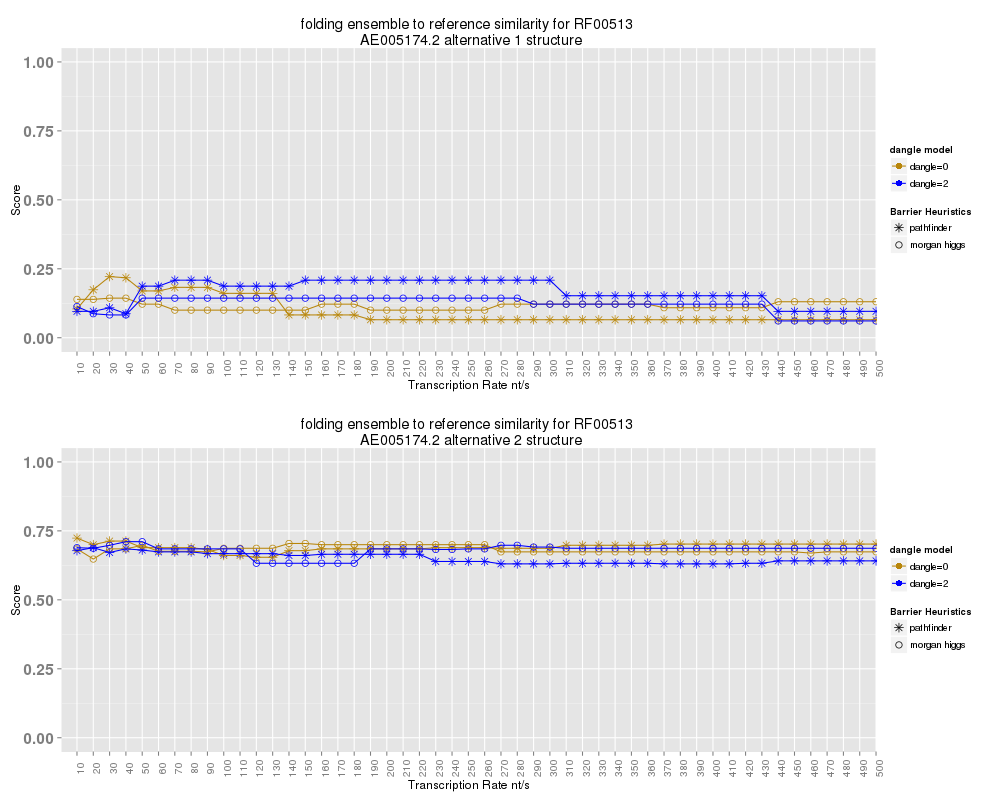
\includegraphics[width=0.9\textwidth]{./pictures/basePairDiversity/TimeDepended/forAlignment/RF00513.png}
%\caption{base-pair diversity for \texttt{trpL} family. \texttt{Kinwalker} parameter-set used : \texttt{findpath} and dangle option 2. Rather constant diversity over all \texttt{Kinwalker} parameters.}
%\label{fig:base-pair diversity for alignment RF00513}
%\end{figure}
%			
%\begin{figure}[ht] 
%\centering
%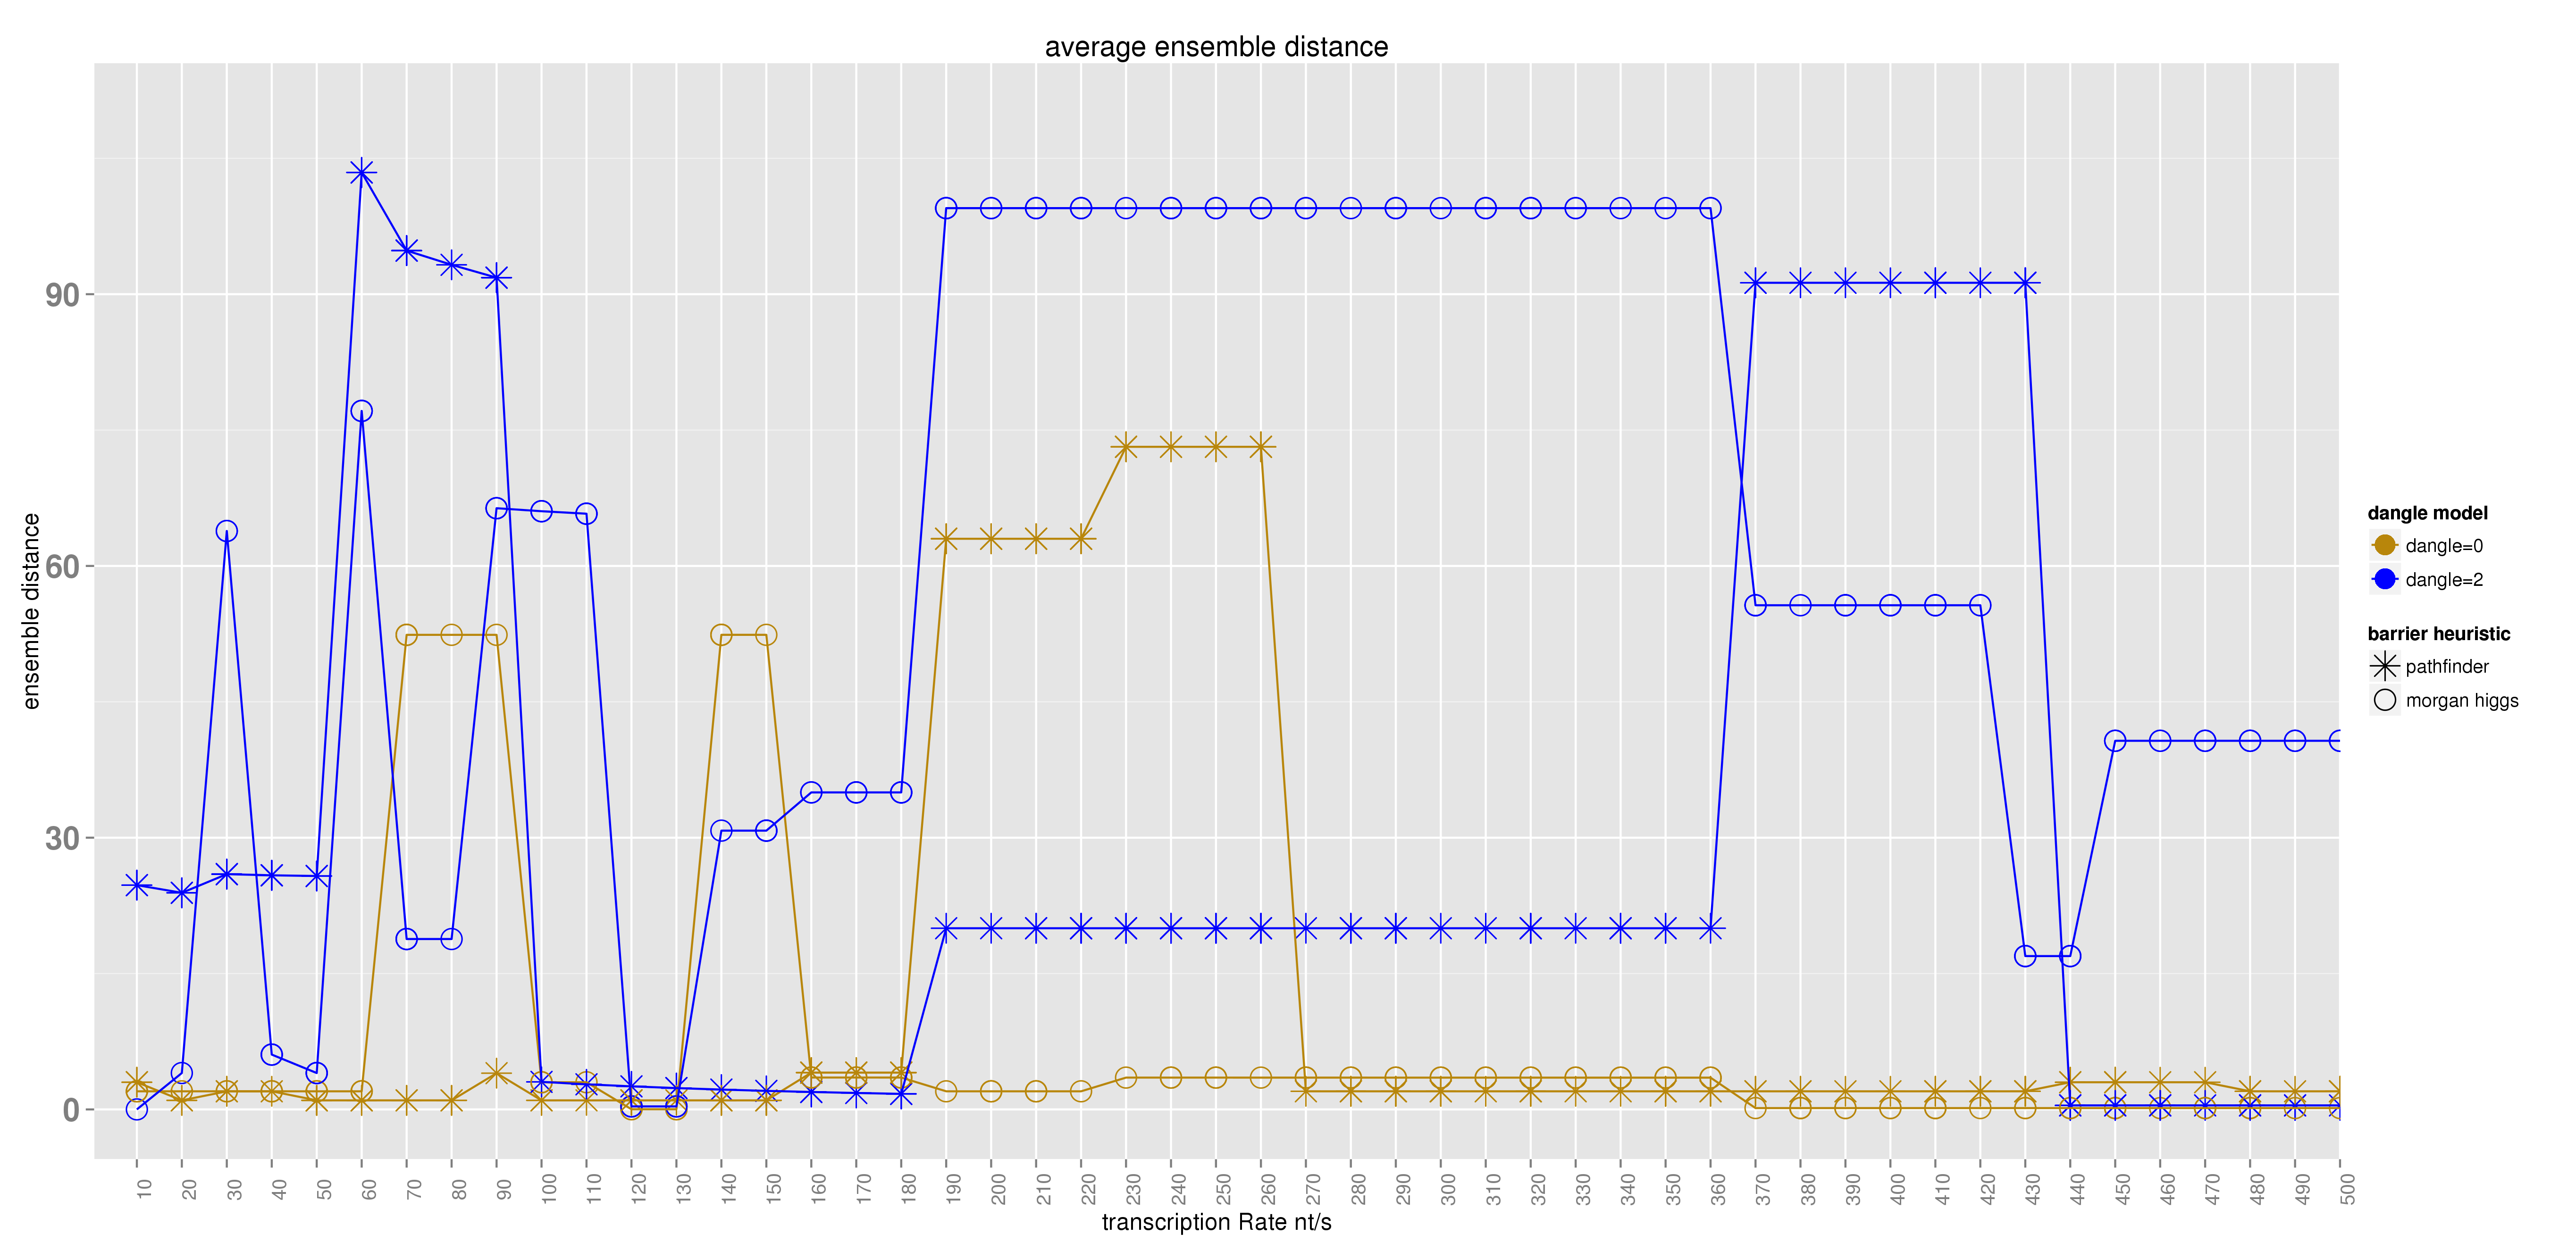
\includegraphics[width=0.9\textwidth]{./pictures/basePairDiversity/TimeDepended/forAlignment/RF00010.png}
%\caption{base-pair diversity for \texttt{RNaseP} family. \texttt{Kinwalker} parameter-set used : \texttt{findpath} and dangle option 2. A lot of diversity changes if transcription rates below 120 nt/s were used.}
%\label{fig:base-pair diversity for alignment RF00010}
%\end{figure}
				
\FloatBarrier	
\section{ensemble diversity} \label{result:ensemble diversity}

The ensemble diversity score extended with base-pair probabilities instead of ensemble probabilities can be used to determine 
the diversity of base-pairs along the folding trajectory. Due to choosing of $\frac{\Delta
  Time_{ij}}{period}$ as measurement for the probability of base-pair (i,j) to appear, the time period can be used to investigate base-pair diversity at varying stages of co-transcriptional folding and afterwards.
For each reference sequences of the three families the ensemble diversity
was calculated for three different time periods exceeding transcription end
(i.e. $2,5,10 \times$transcription time) (fig.~\ref{fig:ensemble_diversity_X01074.1}, \ref{fig:ensemble_diversity_CP001509.3},  \ref{fig:ensemble_diversity_AE005174.2}). 

Ensemble diversity for \texttt{SRP} reference sequence shows no difference if time periods of $2,5,10 \times$transcription time were used. Furthermore, the ensemble diversity is extremely homogenous, except two outliers (i.e. diversity increase at 20 nt/s with \texttt{findpath} and dangle option $0$ as well as with transcription rates ranging from 27 to 300 nt/s with \texttt{findpath} and dangle option 2). Apart from these, \texttt{Kinwalker} parameters have very little influence  at the ensemble diversity for the \texttt{SRP} reference sequence.


Ensemble diversity for \texttt{trpL} reference sequence shows differences between the time periods used, if and only if \texttt{findpath} algorithm with dangle option 0 is used. There is no difference in the resulting ensemble diversity with every other \texttt{Kinwalker} parameter combination.
An ensemble diversity drop is noticed at transcription rates of 140 to 150 nt/s calculated with \texttt{findpath} and dangle $0$ option if time periods of 2 or 5$\times$ transcription rates are used.
By using the time period of 10$\times$ transcription rate the drop of ensemble diversity starts at the same transcription rates, but is not as sharp as with 2 or 5$\times$ transcription rate, and slowly decreasing until transcription rate of 330 nt/s.

Ensemble diversity for \texttt{RNaseP} reference sequence shows differences between the time periods used, if and only if \texttt{findpath} algorithm with dangle option 2 is used. Overall there is an extremely low diverse behavior of the ensemble, except a big diversity increases at transcription rates ranging from 60 to 90 nt/s if \texttt{findpath} and dangle option 2 are used. 
The only difference between 5$\times$ transcription time and 10$\times$ transcription time is an increase in ensemble diversity with a transcription rate of 10 nt/s with \texttt{findpath} algorithm and dangle option 2.


\begin{figure}[ht]
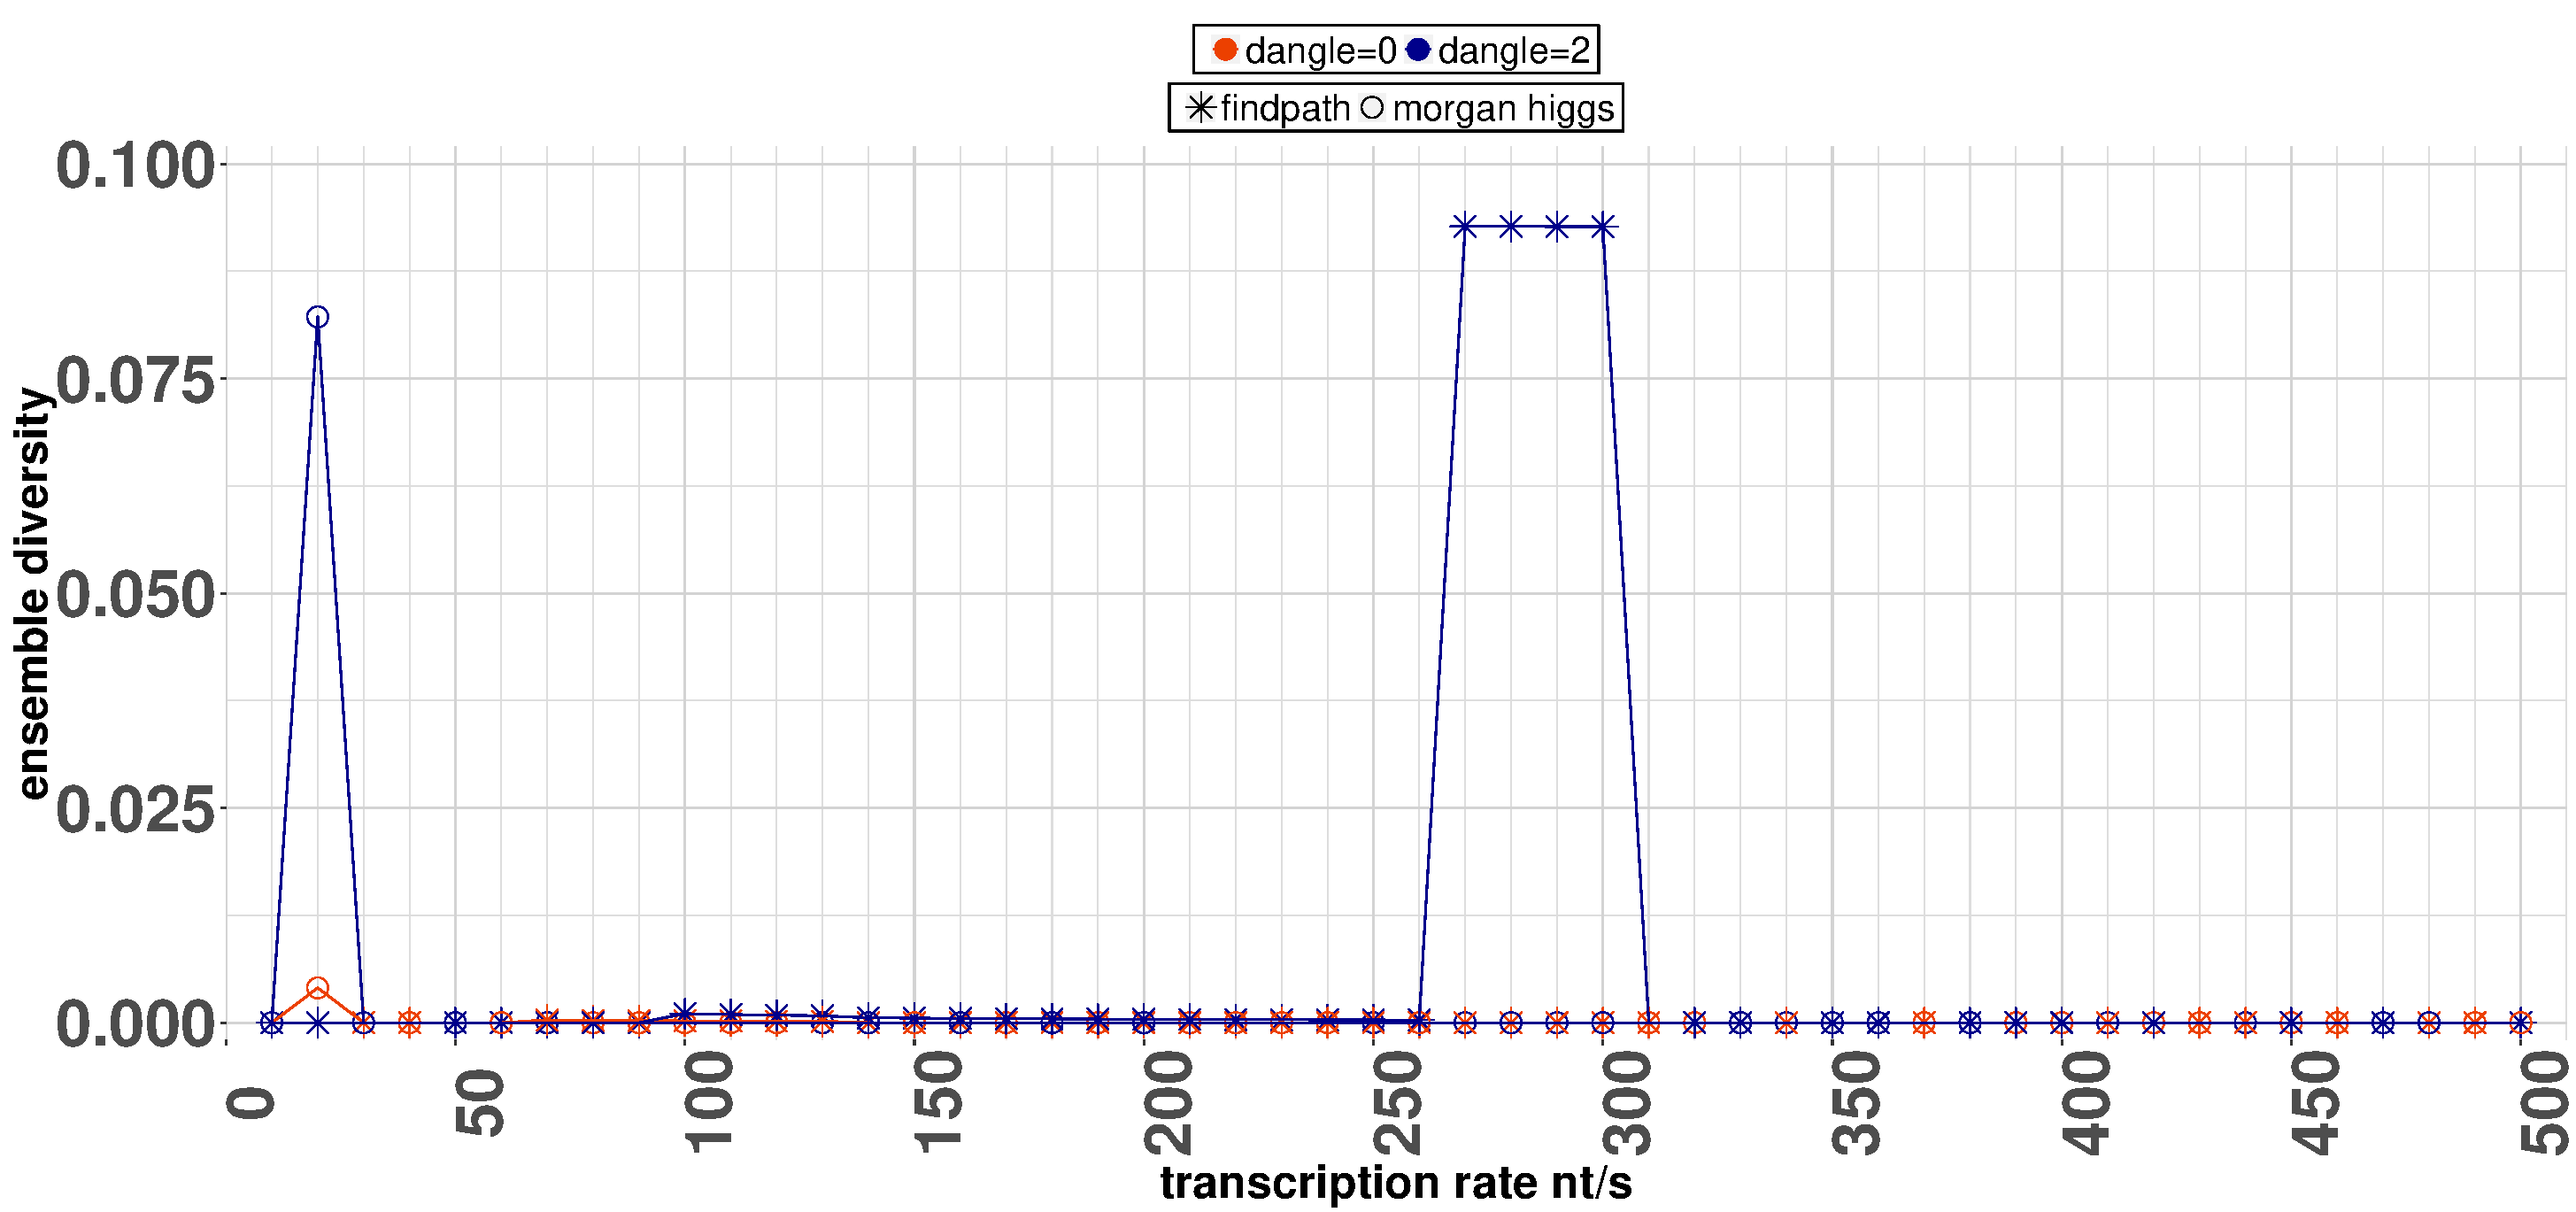
\includegraphics[width=0.9\textwidth]{./pictures/ensembleDiversity/SRP2510.pdf}
\caption{{\bf ensemble diversity of \texttt{SRP} reference sequence.}
No difference between $2,5,10 \times$transcription time. Extremely constant ensemble diversity except two increases at 20 nt/s with \texttt{findpath} and dangle option $0$ as well as with transcription rates ranging from 270 to 300 nt/s with \texttt{findpath} and dangle option 2.
}
\label{fig:ensemble_diversity_X01074.1}
\end{figure}	


\begin{figure}[ht]
\begin{tabular}{l}
(a) $2 \times$transcription time \\
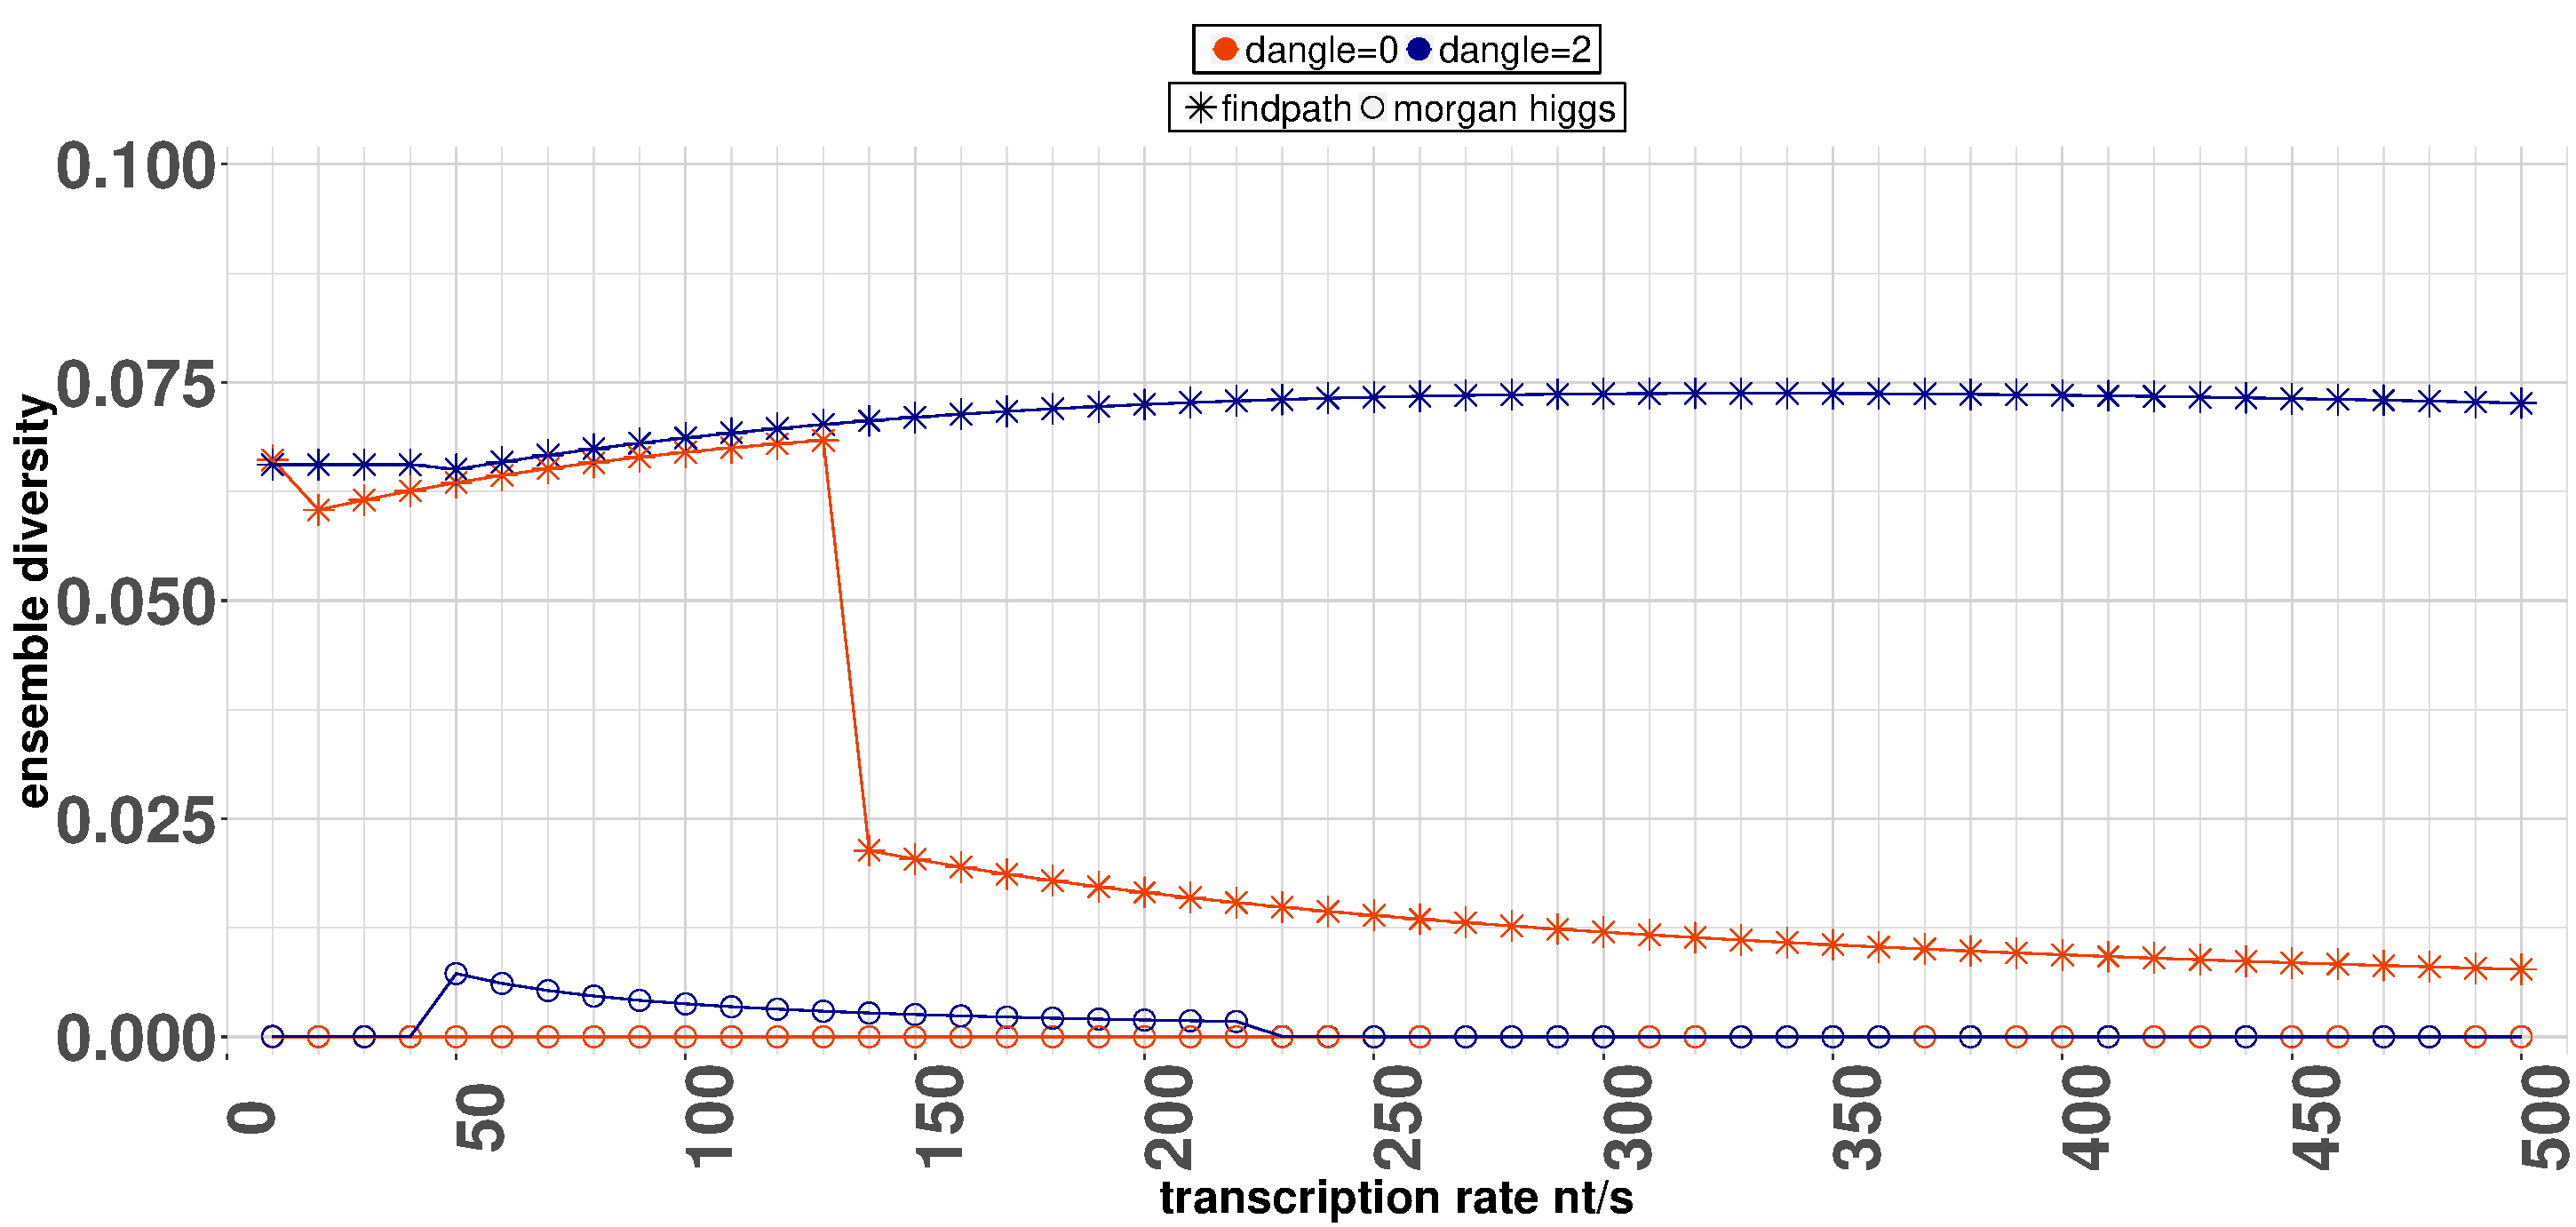
\includegraphics[width=0.9\textwidth]{./pictures/ensembleDiversity/trpL2.pdf}\\
\hline
(b) $5 \times$transcription time \\
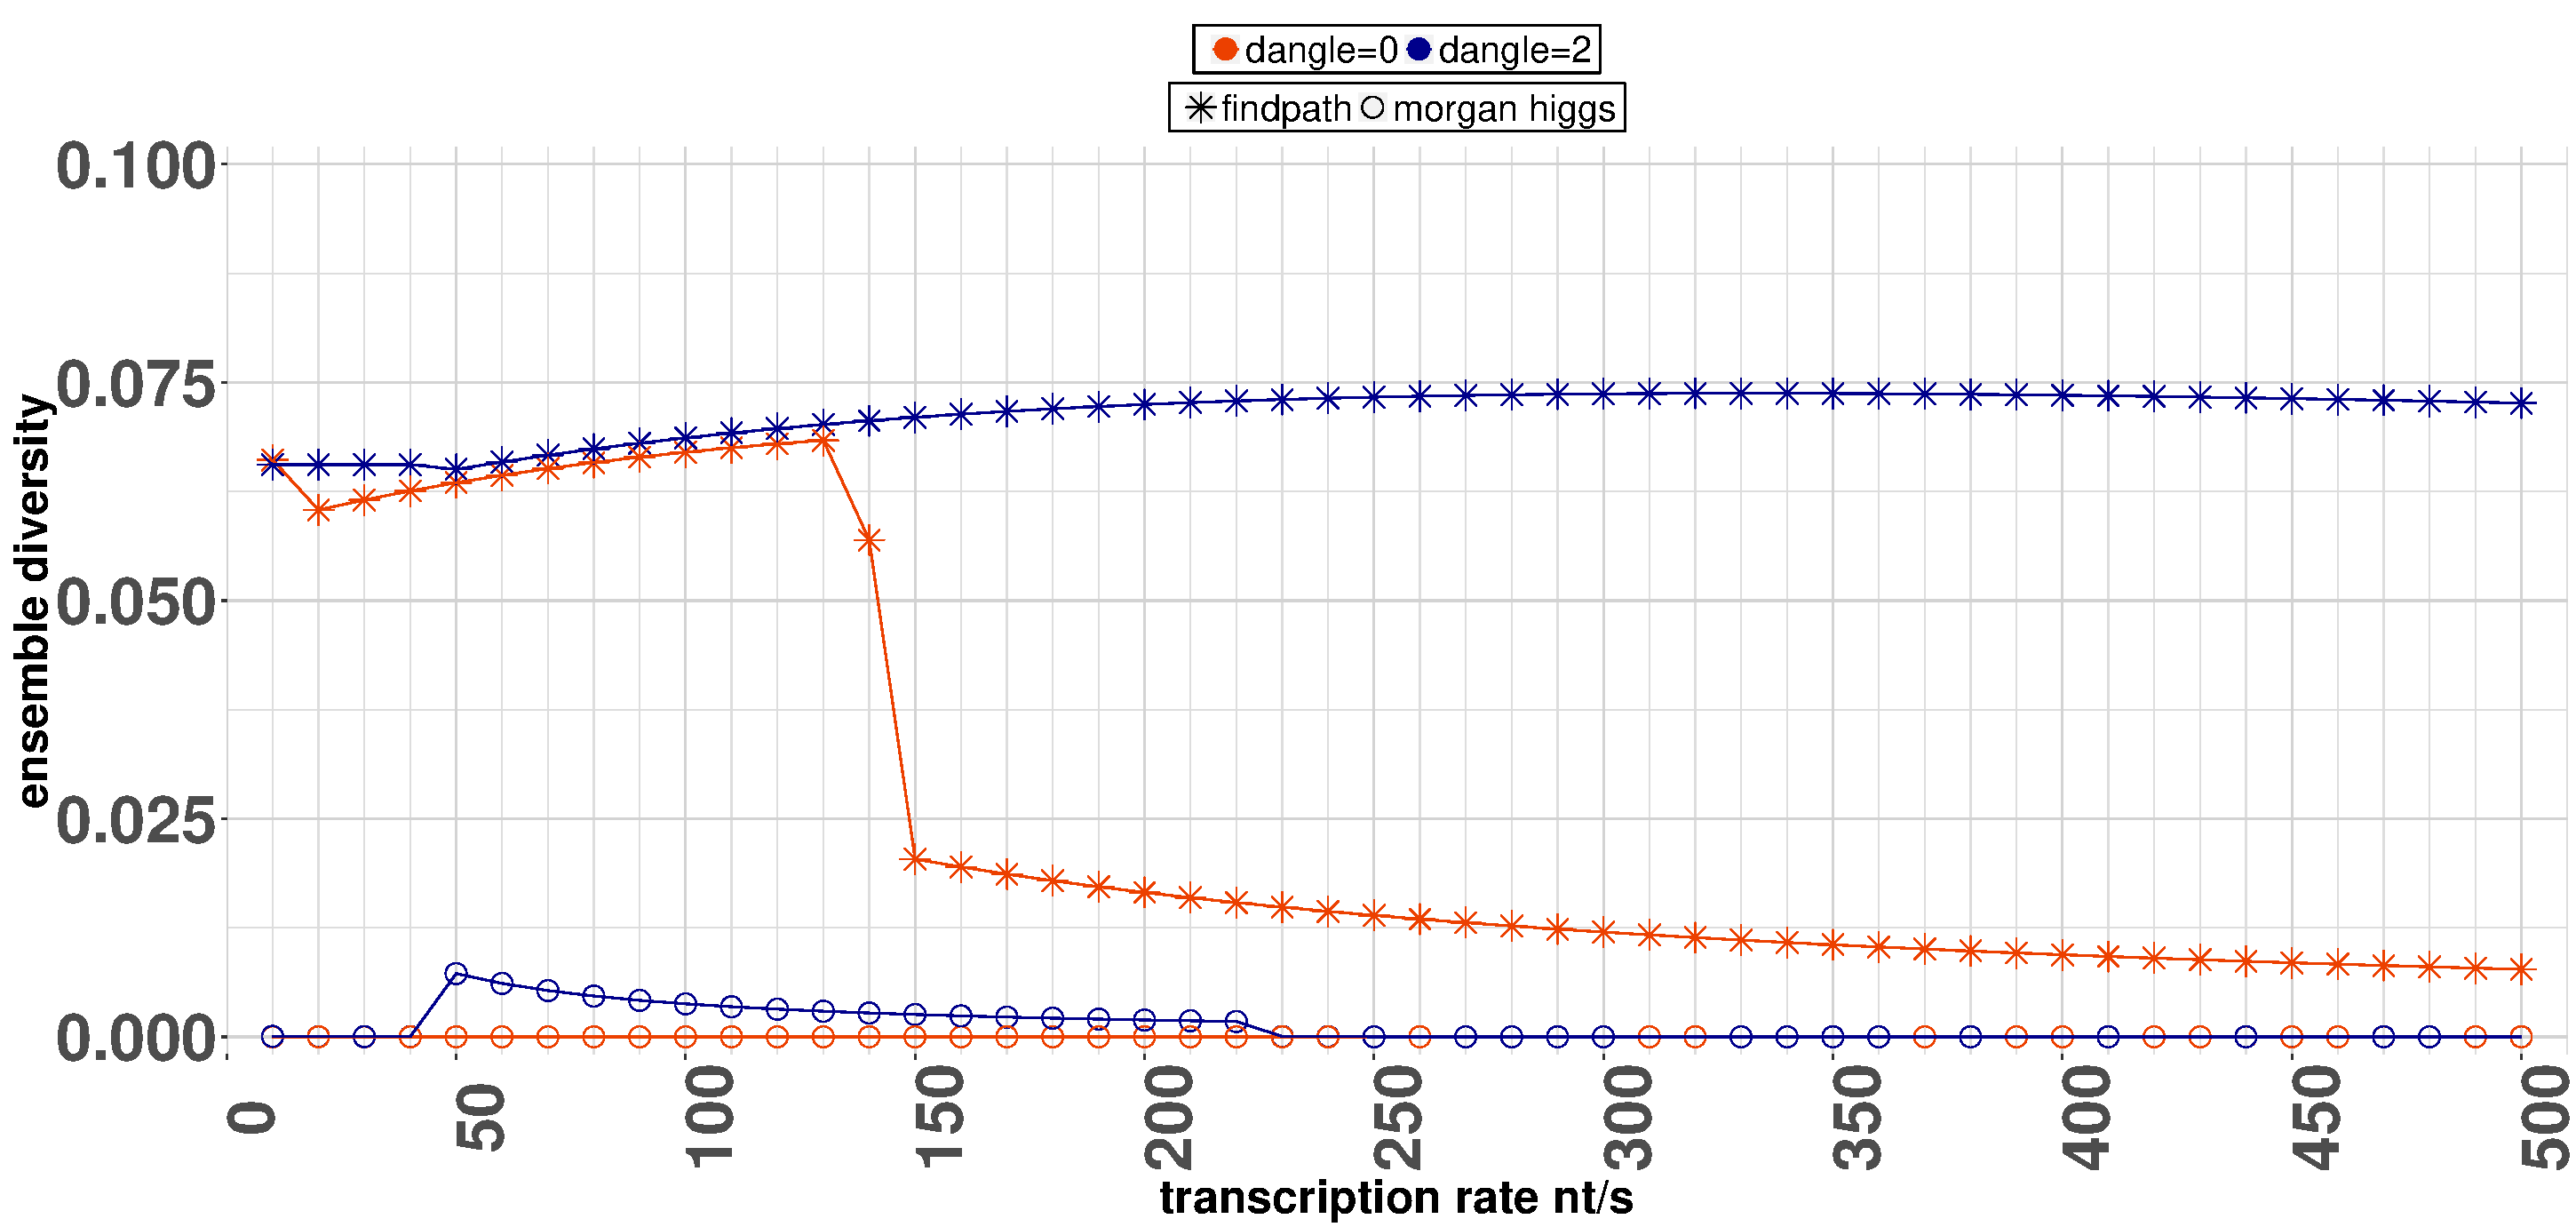
\includegraphics[width=0.9\textwidth]{./pictures/ensembleDiversity/trpL5.pdf}\\
\hline
(c) $10 \times$transcription time \\
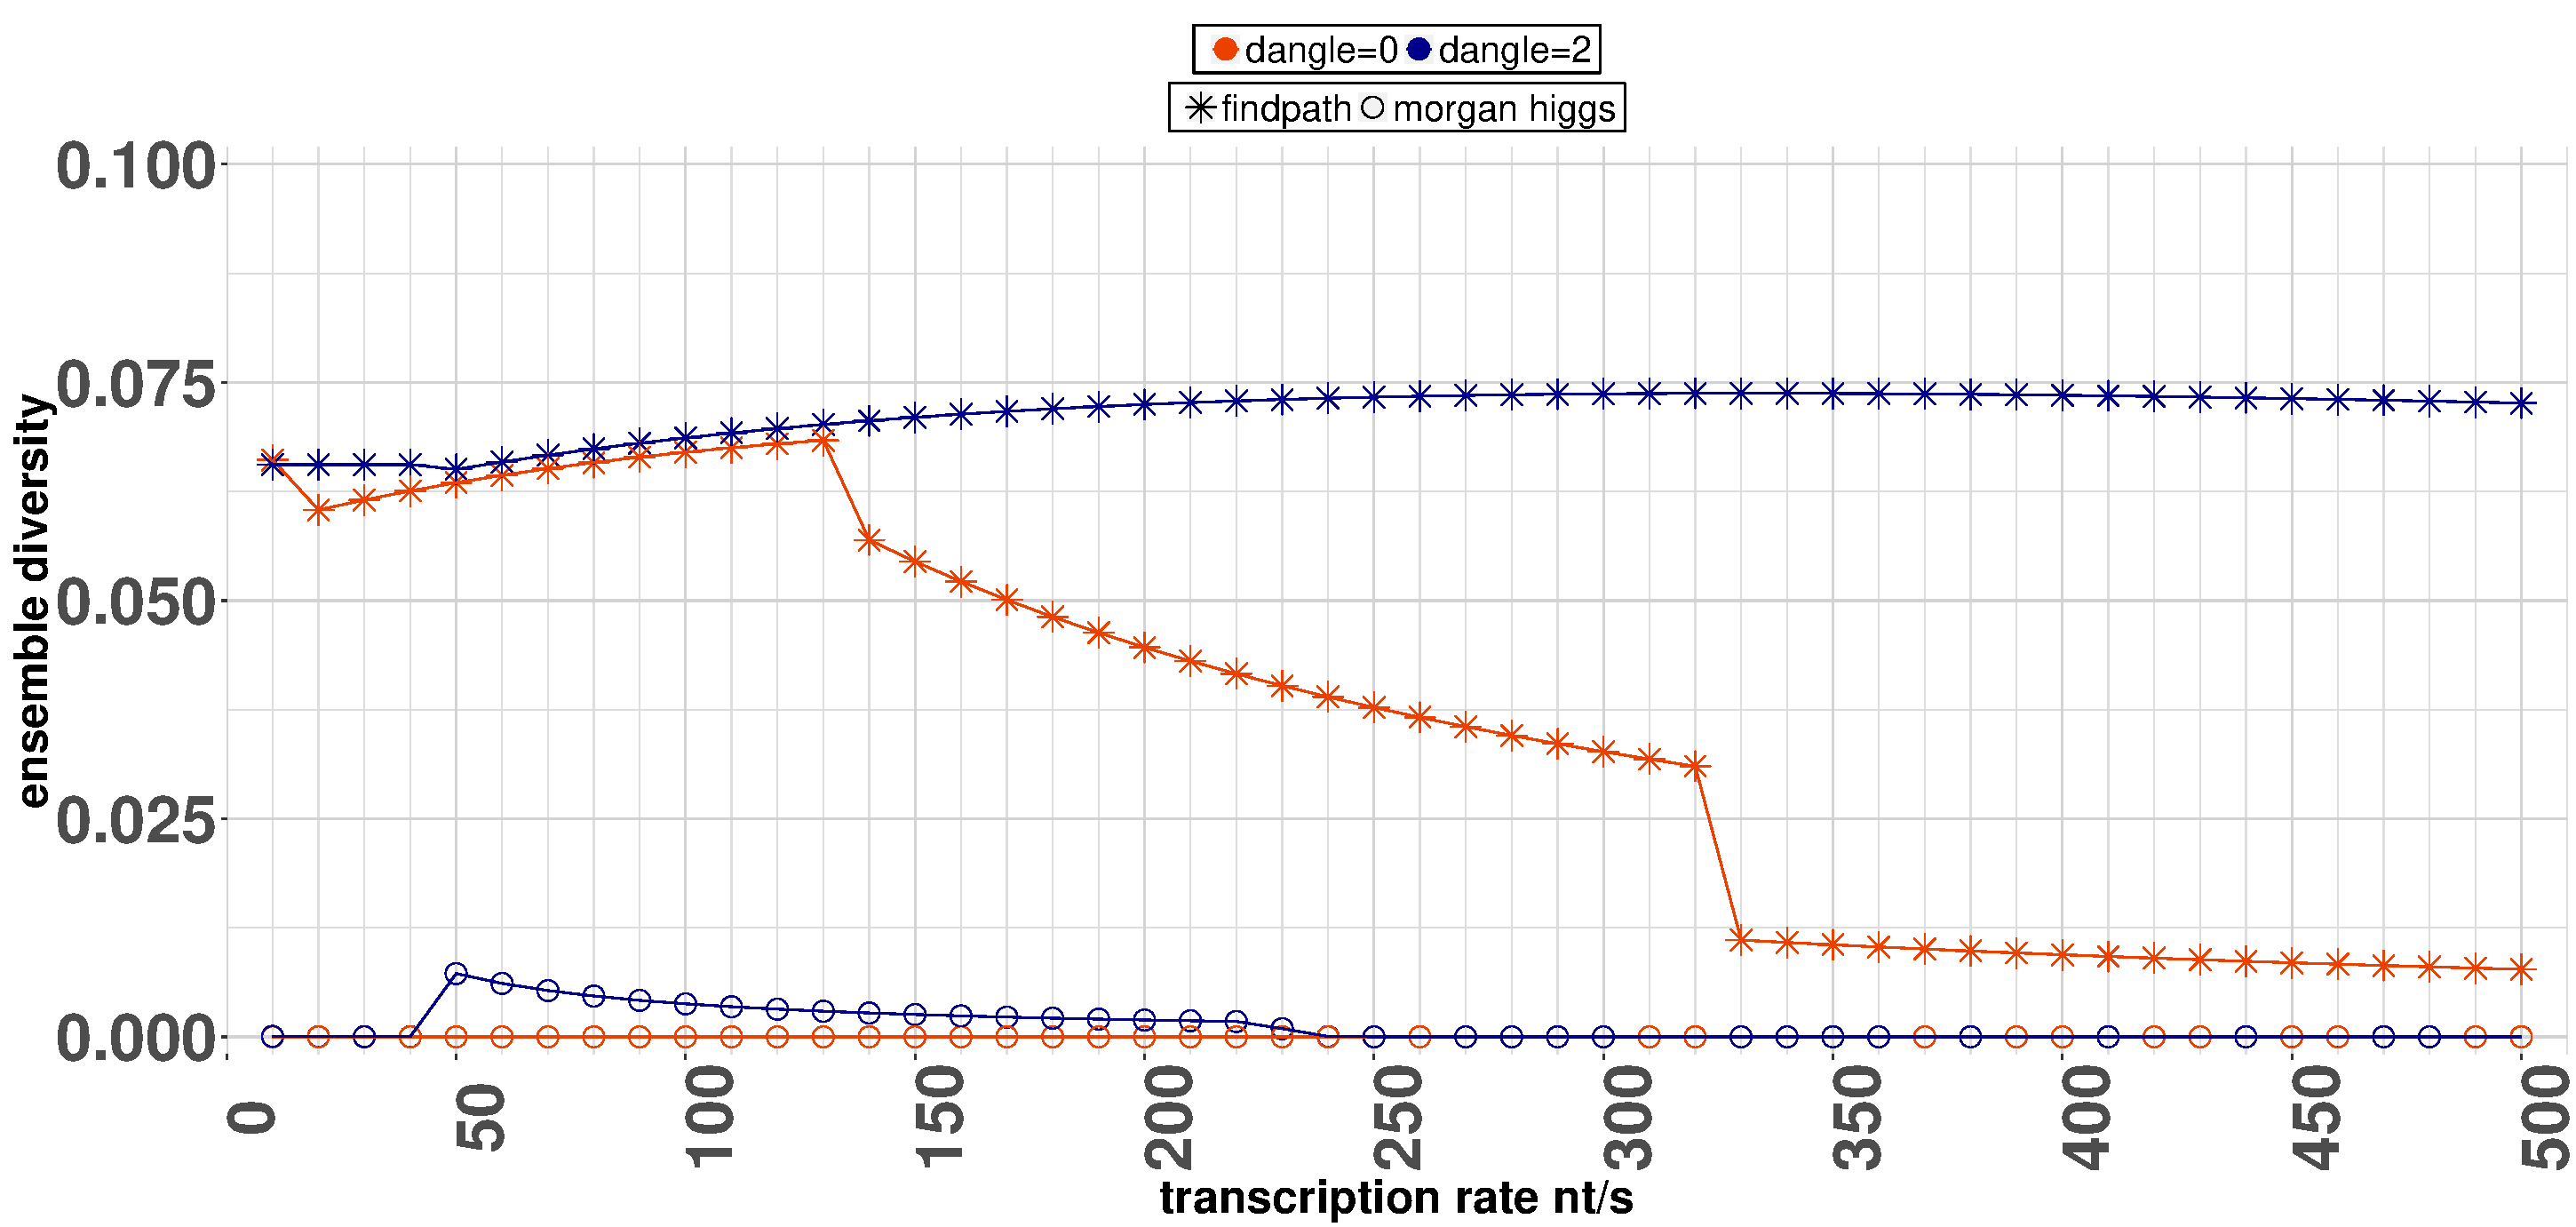
\includegraphics[width=0.9\textwidth]{./pictures/ensembleDiversity/trpL10.pdf}\\
\end{tabular}
\caption{{\bf ensemble diversity of \texttt{trpL} reference sequence}.
ensemble diversity of \texttt{trpL} reference sequence with time period of (a): $2\times$transcription time, (b): $5\times$transcription time, (c): $10\times$transcription time. An ensemble diversity drop is noticed at transcription rates of 140 to 150 nt/s calculated with \texttt{findpath} and dangle $0$ option if time period (a) or (b) is used.
By using the time period of (c) the drop of ensemble diversity starts at the same transcription rate, but is not as sharp as with (a) and (b) and is slowly decreasing till transcription rate of 330 nt/s }
\label{fig:ensemble_diversity_AE005174.2}
\end{figure}

\begin{figure}[ht]
\begin{tabular}{l}
 (a) 2 or 5 $\times$ transcription time \\
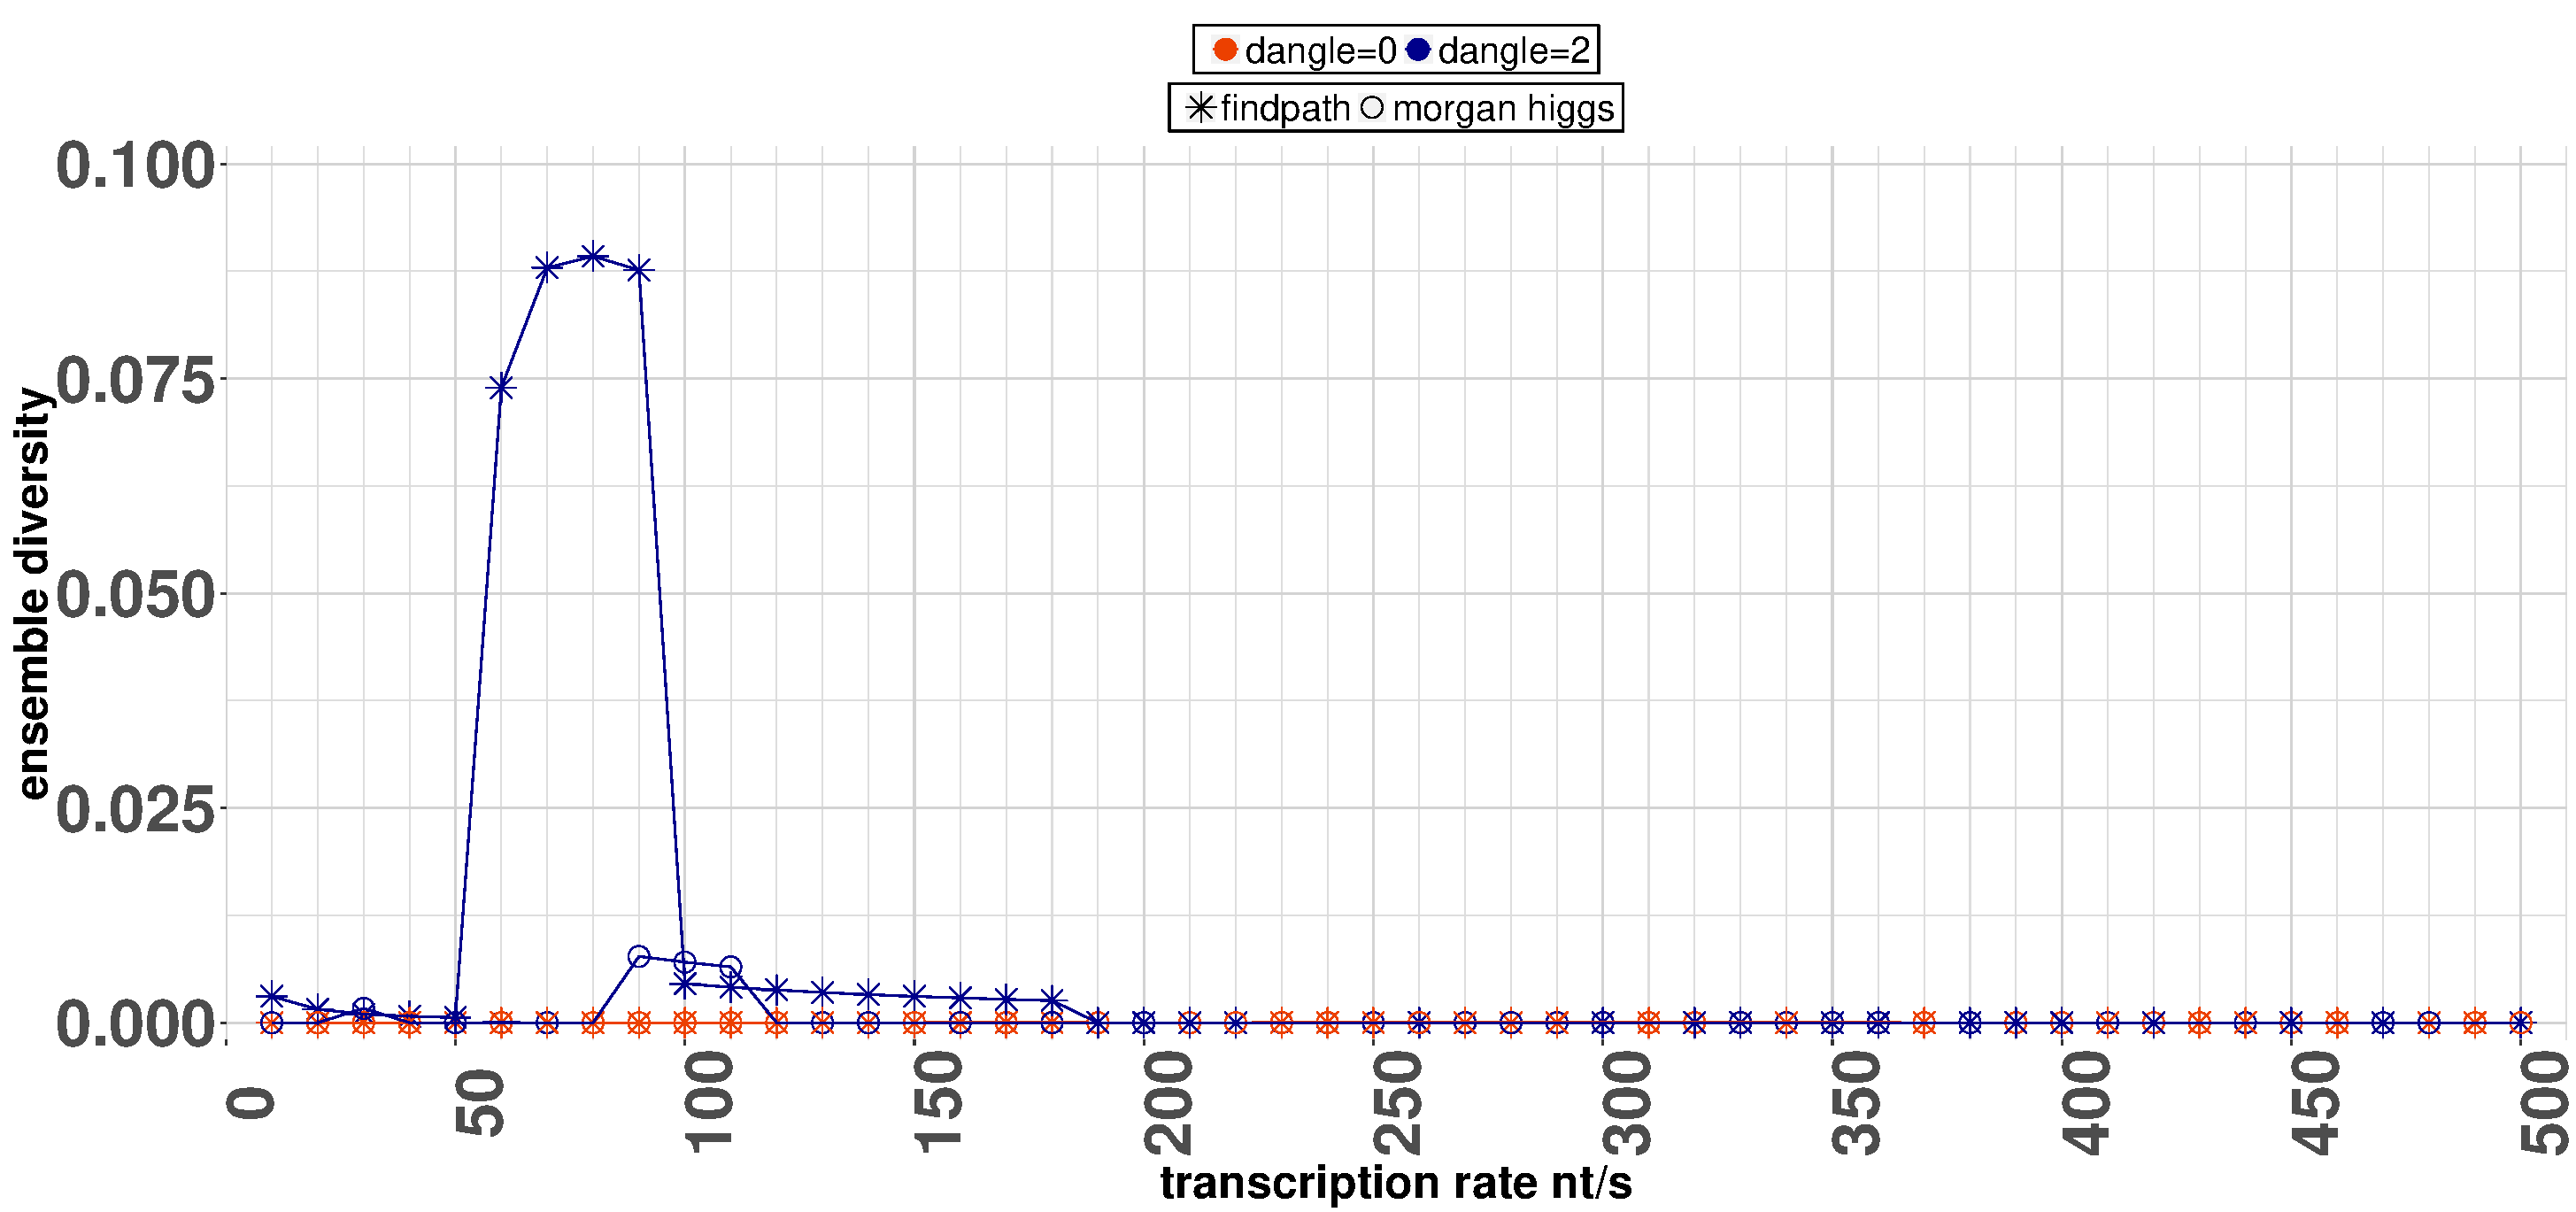
\includegraphics[width=0.9\textwidth]{./pictures/ensembleDiversity/RNaseP25.pdf}\\
\hline
(b) 10$\times$transcription time \\
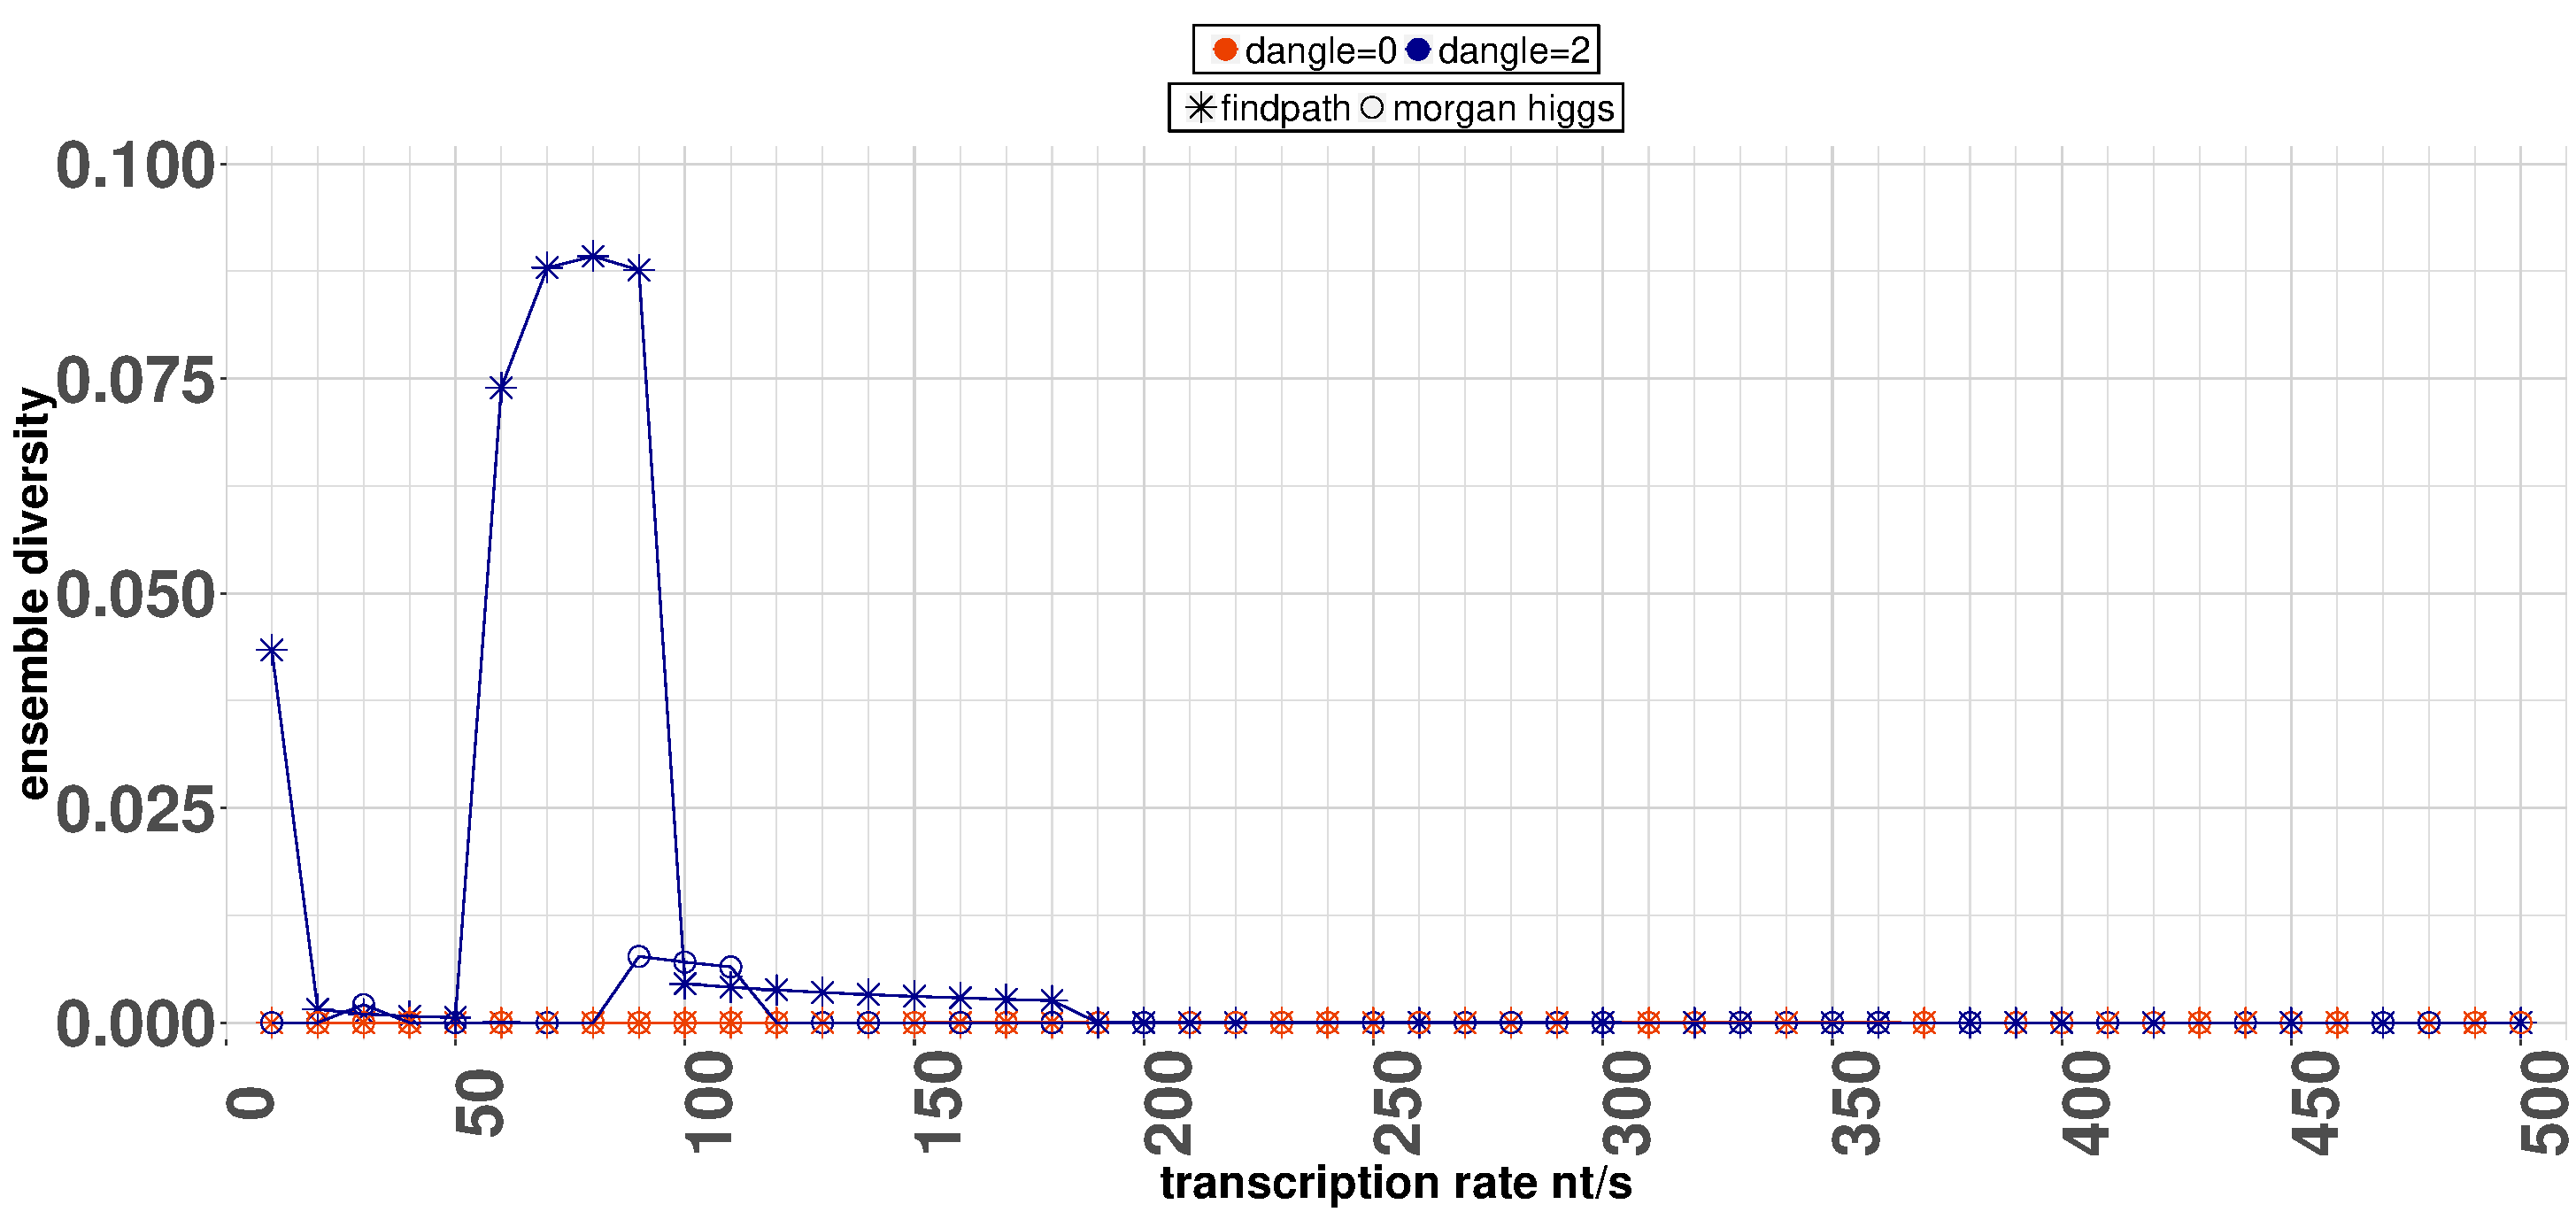
\includegraphics[width=0.9\textwidth]{./pictures/ensembleDiversity/RNaseP10.pdf}\\
\end{tabular}
\caption{{\bf ensemble diversity of \texttt{RNaseP} reference sequence}.
ensemble diversity of \texttt{RNaseP} reference sequence with time period of (a): $2,5\times$transcription time, (b): 10$\times$transcription time.
Extreme low diverse behavior of the ensemble, except a big diversity increases at transcription rates ranging from 60 to 90 nt/s if \texttt{findpath} and dangle option 2 are used. 
(b) Increase in diversity with transcription rate of 10 nt/s and \texttt{findpath} with dangle option 2 
}
\label{fig:ensemble_diversity_CP001509.3}
\end{figure}
	
\FloatBarrier	
\section{Ensemble Distance}
The ensemble distance analyzes weather a substructure of a reference structure is part of the folding trajectory of another sequence, by measuring the percentage of reference structure base-pairs also found in the folding trajectory.
Ensemble distance is extended by adding time factors and is now the expected distance between the predicted trajectory and the reference structure\cite{EnsembleDistance}.
Equation: \ref{eq:ensemble distance} was used to calculate the following results.

Five \textit{in vitro} analyzed reference structures for the three chosen
RNA families were compared to folding trajectories of their corresponding
sequences (fig.~\ref{fig:ensembleDistanceSRP},
\ref{fig:ensembleDistanceTRP}, \ref{fig:ensembleDistanceRNAseP}). In theory,
the ideal case would be a folding trajectory that leads directly into the
reference structure without resulting in energetically stable intermediate
structures, which in turn could prevent refolding into the reference structure. 
Here, similar to the base-pair diversity only dangle option 2 and \texttt{findpath} algorithm were used for ensemble distance calculations.
An ensemble distance of 1 is observed, if not even one reference structure base-pair is found in the given folding trajectory.
Likewise, an ensemble distance of 0 indicates that every reference structure base-pair is found in the given folding trajectory.

%Ensemble distances for SRP, \texttt{trpL} and \texttt{RNaseP} families resulting with more distance variations at lower transcription rates and more constant behavior at higher transcription rates.

\texttt{SRP}, \texttt{trpL} and \texttt{RNaseP} families yield more ensemble distance variations at lower transcription rates and more constant behavior at higher transcription rates.

The ensemble distance was calculated for the \texttt{SRP} family to their \texttt{SRP}
functional and \texttt{SRP} transient reference structure.
Both distances show a similar high variation of ensemble distance at lower transcription rates whereby the distance at higher transcription rates is rather constant. Furthermore, a distance drop for both structures is observed at transcription rates ranging from 270 to 300 nt/s.

The ensemble distance was calculated for the \texttt{trpL} family to their terminator and antiterminator reference structure.
The distance to the antiterminator structure is rather constant at higher transcription rates and is more diverse at lower transcripiton rates. An increase in ensemble distance is apparent for many sequences at transcription rate of 300 nt/s.
In contrast, distance to the terminator structure is equally diverse over all transcription rates.

The ensemble distance was calculated for the \texttt{RNaseP} family to their functional reference structure.
More ensemble distance variations occur with lower transcription rates, whereby the distance with higher transcription rates is rather constant.


\begin{figure}
\begin{tabular}{l}
(a) \texttt{SRP} functional \\
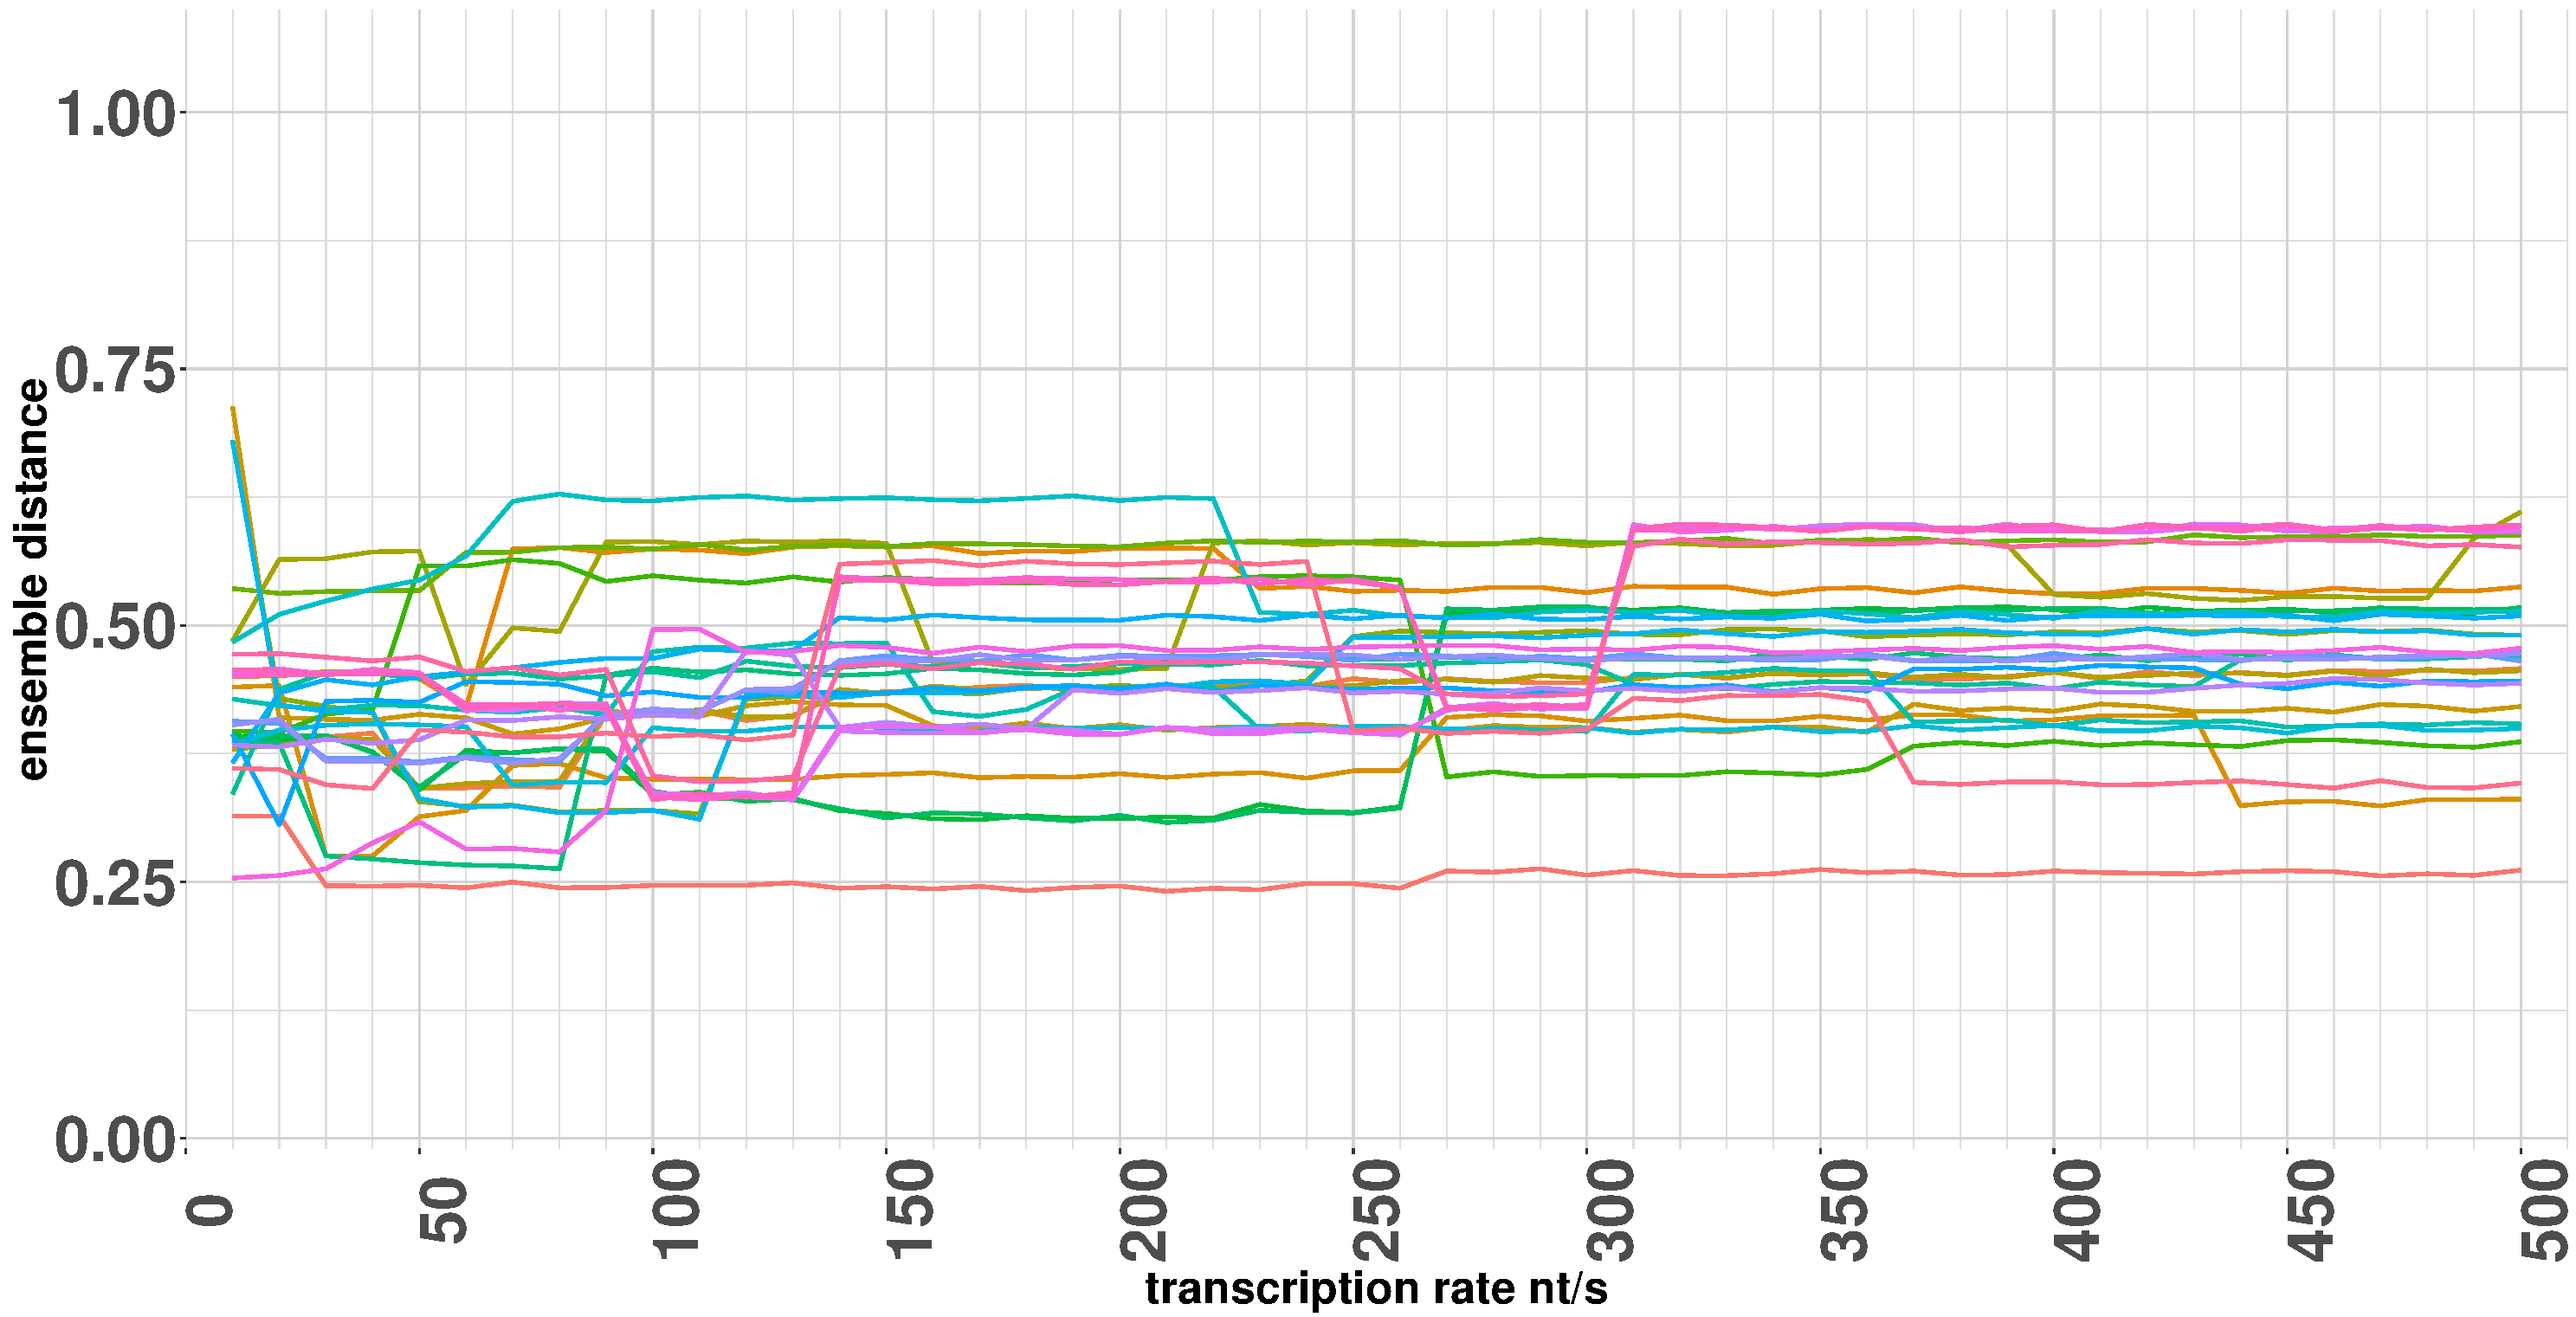
\includegraphics[width=0.9\textwidth]{./pictures/ensembleDistance/ensembleDistance_SRPFunctional.pdf}\\ 
\hline
(b) \texttt{SRP} transient\\
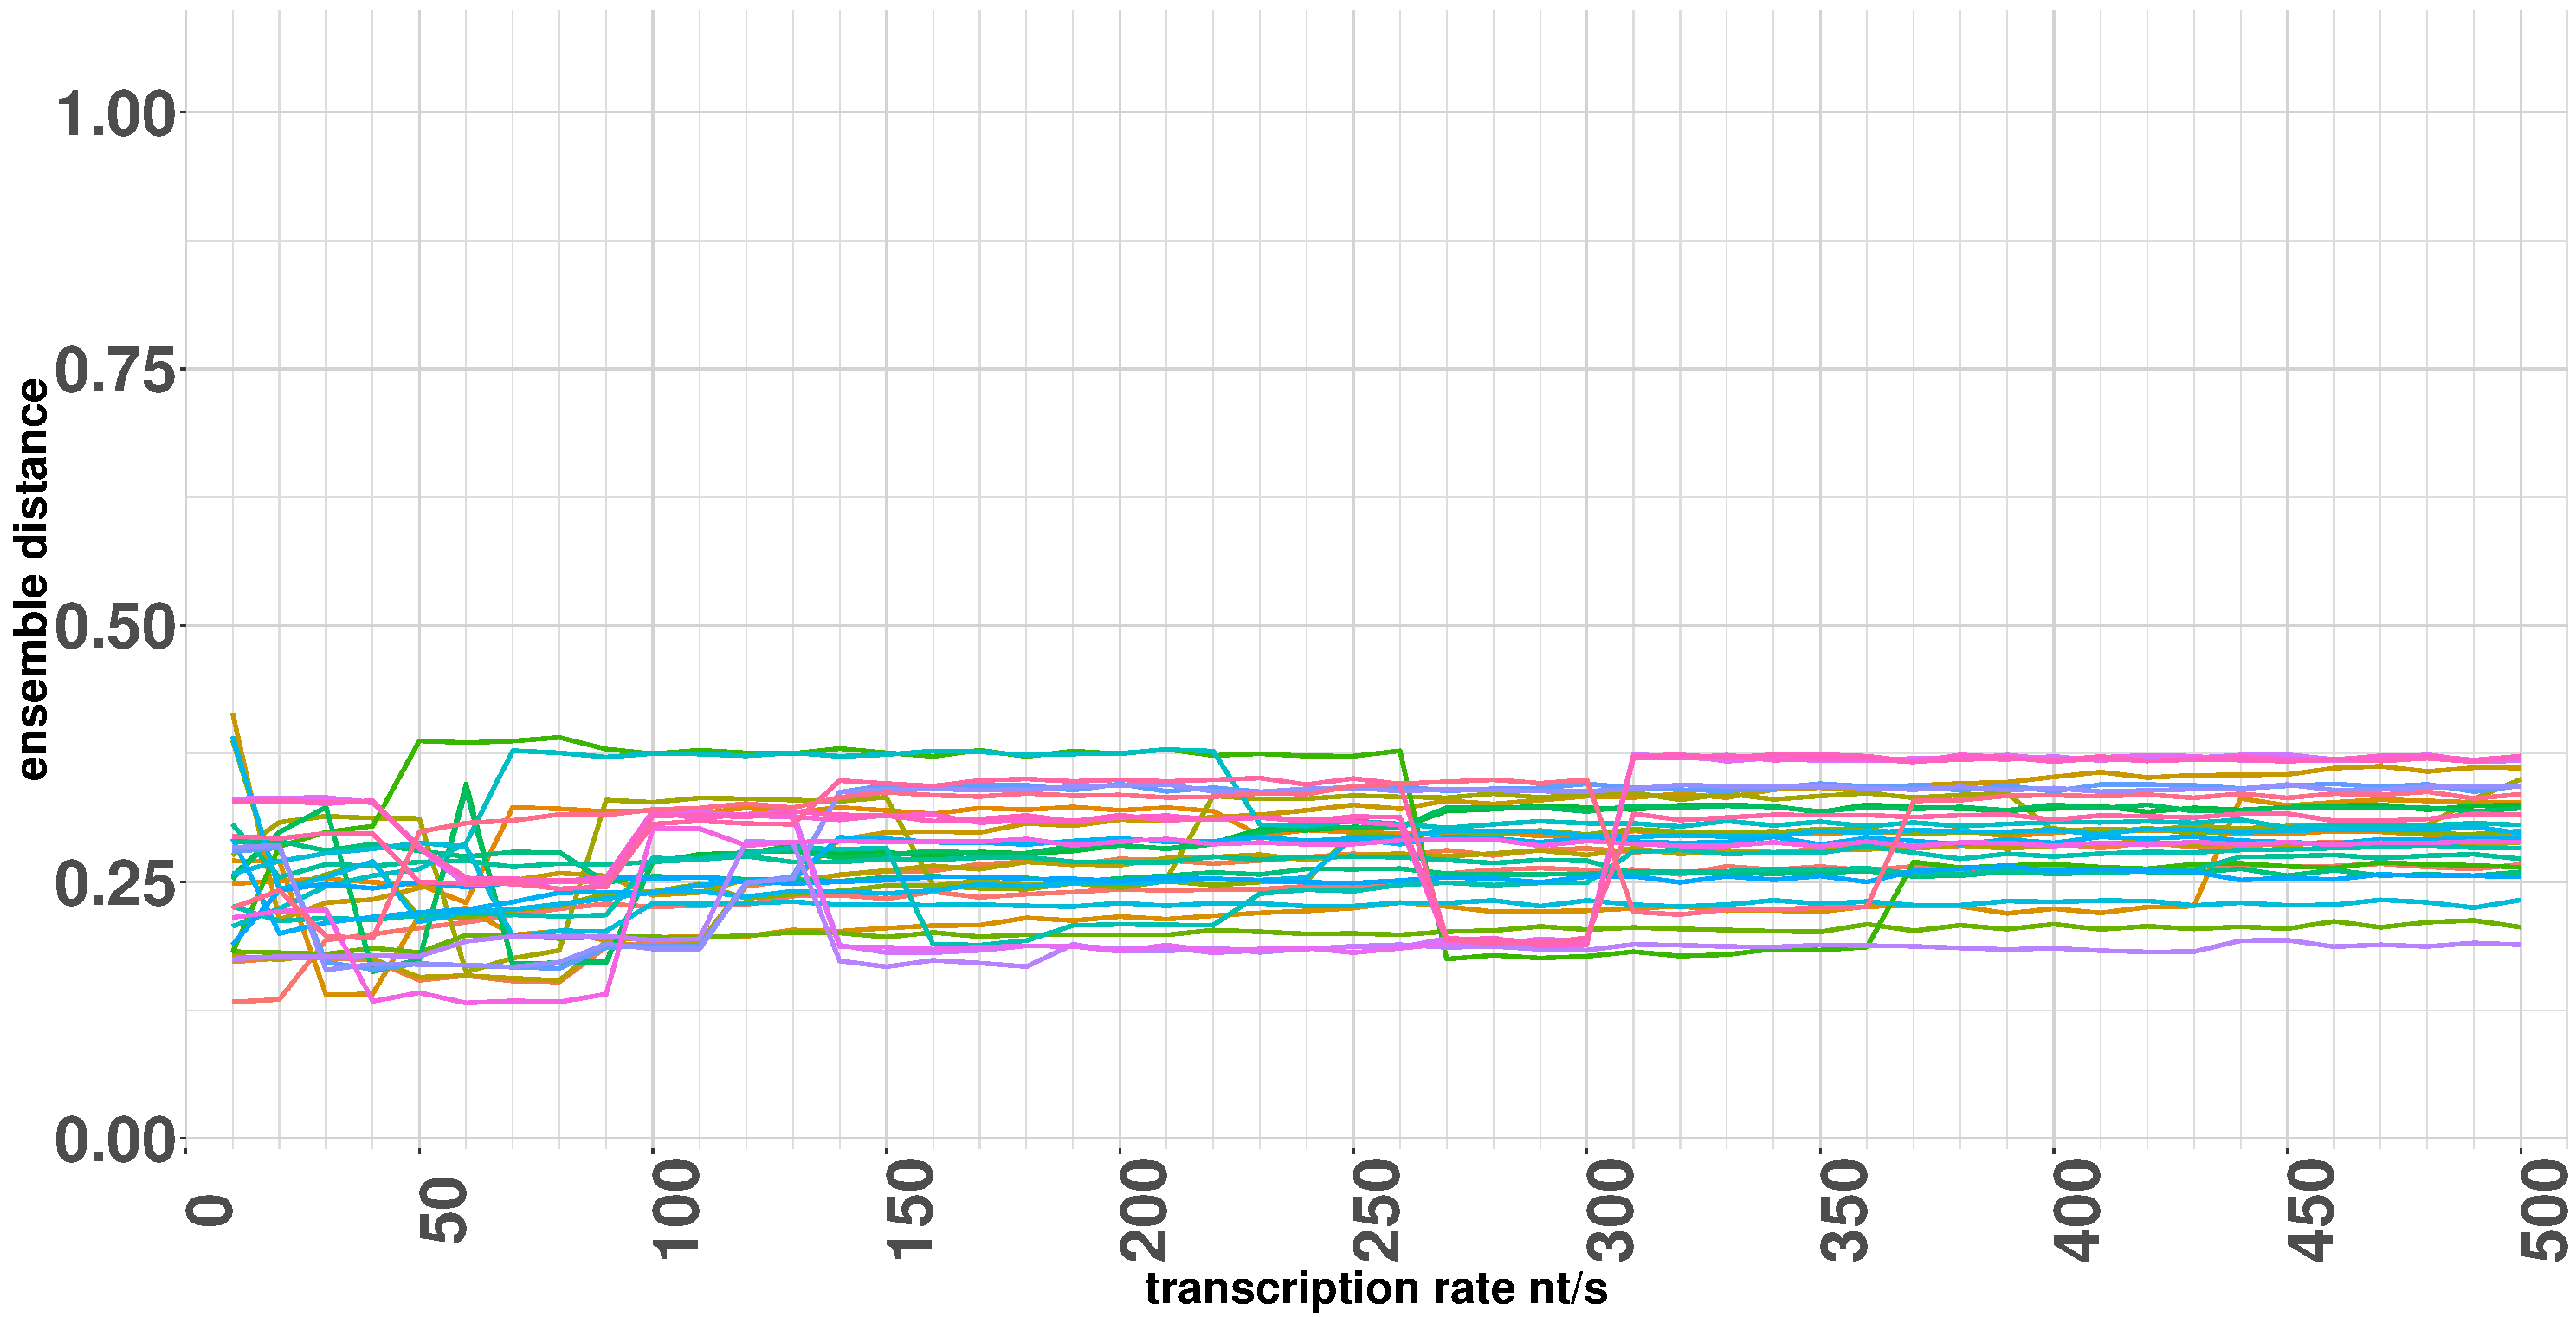
\includegraphics[width=0.9\textwidth]{./pictures/ensembleDistance/ensembleDistance_SRPtransient.pdf}\\
\end{tabular}
\caption{{\bf Ensemble distances of \texttt{SRP} family}
\texttt{findpath} and dangle option 2 were used.
 (a) distance to \texttt{SRP} functional reference structure.
 (b) distance to \texttt{SRP} transient reference structure. 
 }
\label{fig:ensembleDistanceSRP}
\end{figure}			
 							

		
\begin{figure}
\begin{tabular}{l}
(a) \texttt{trpL} antiterminator \\
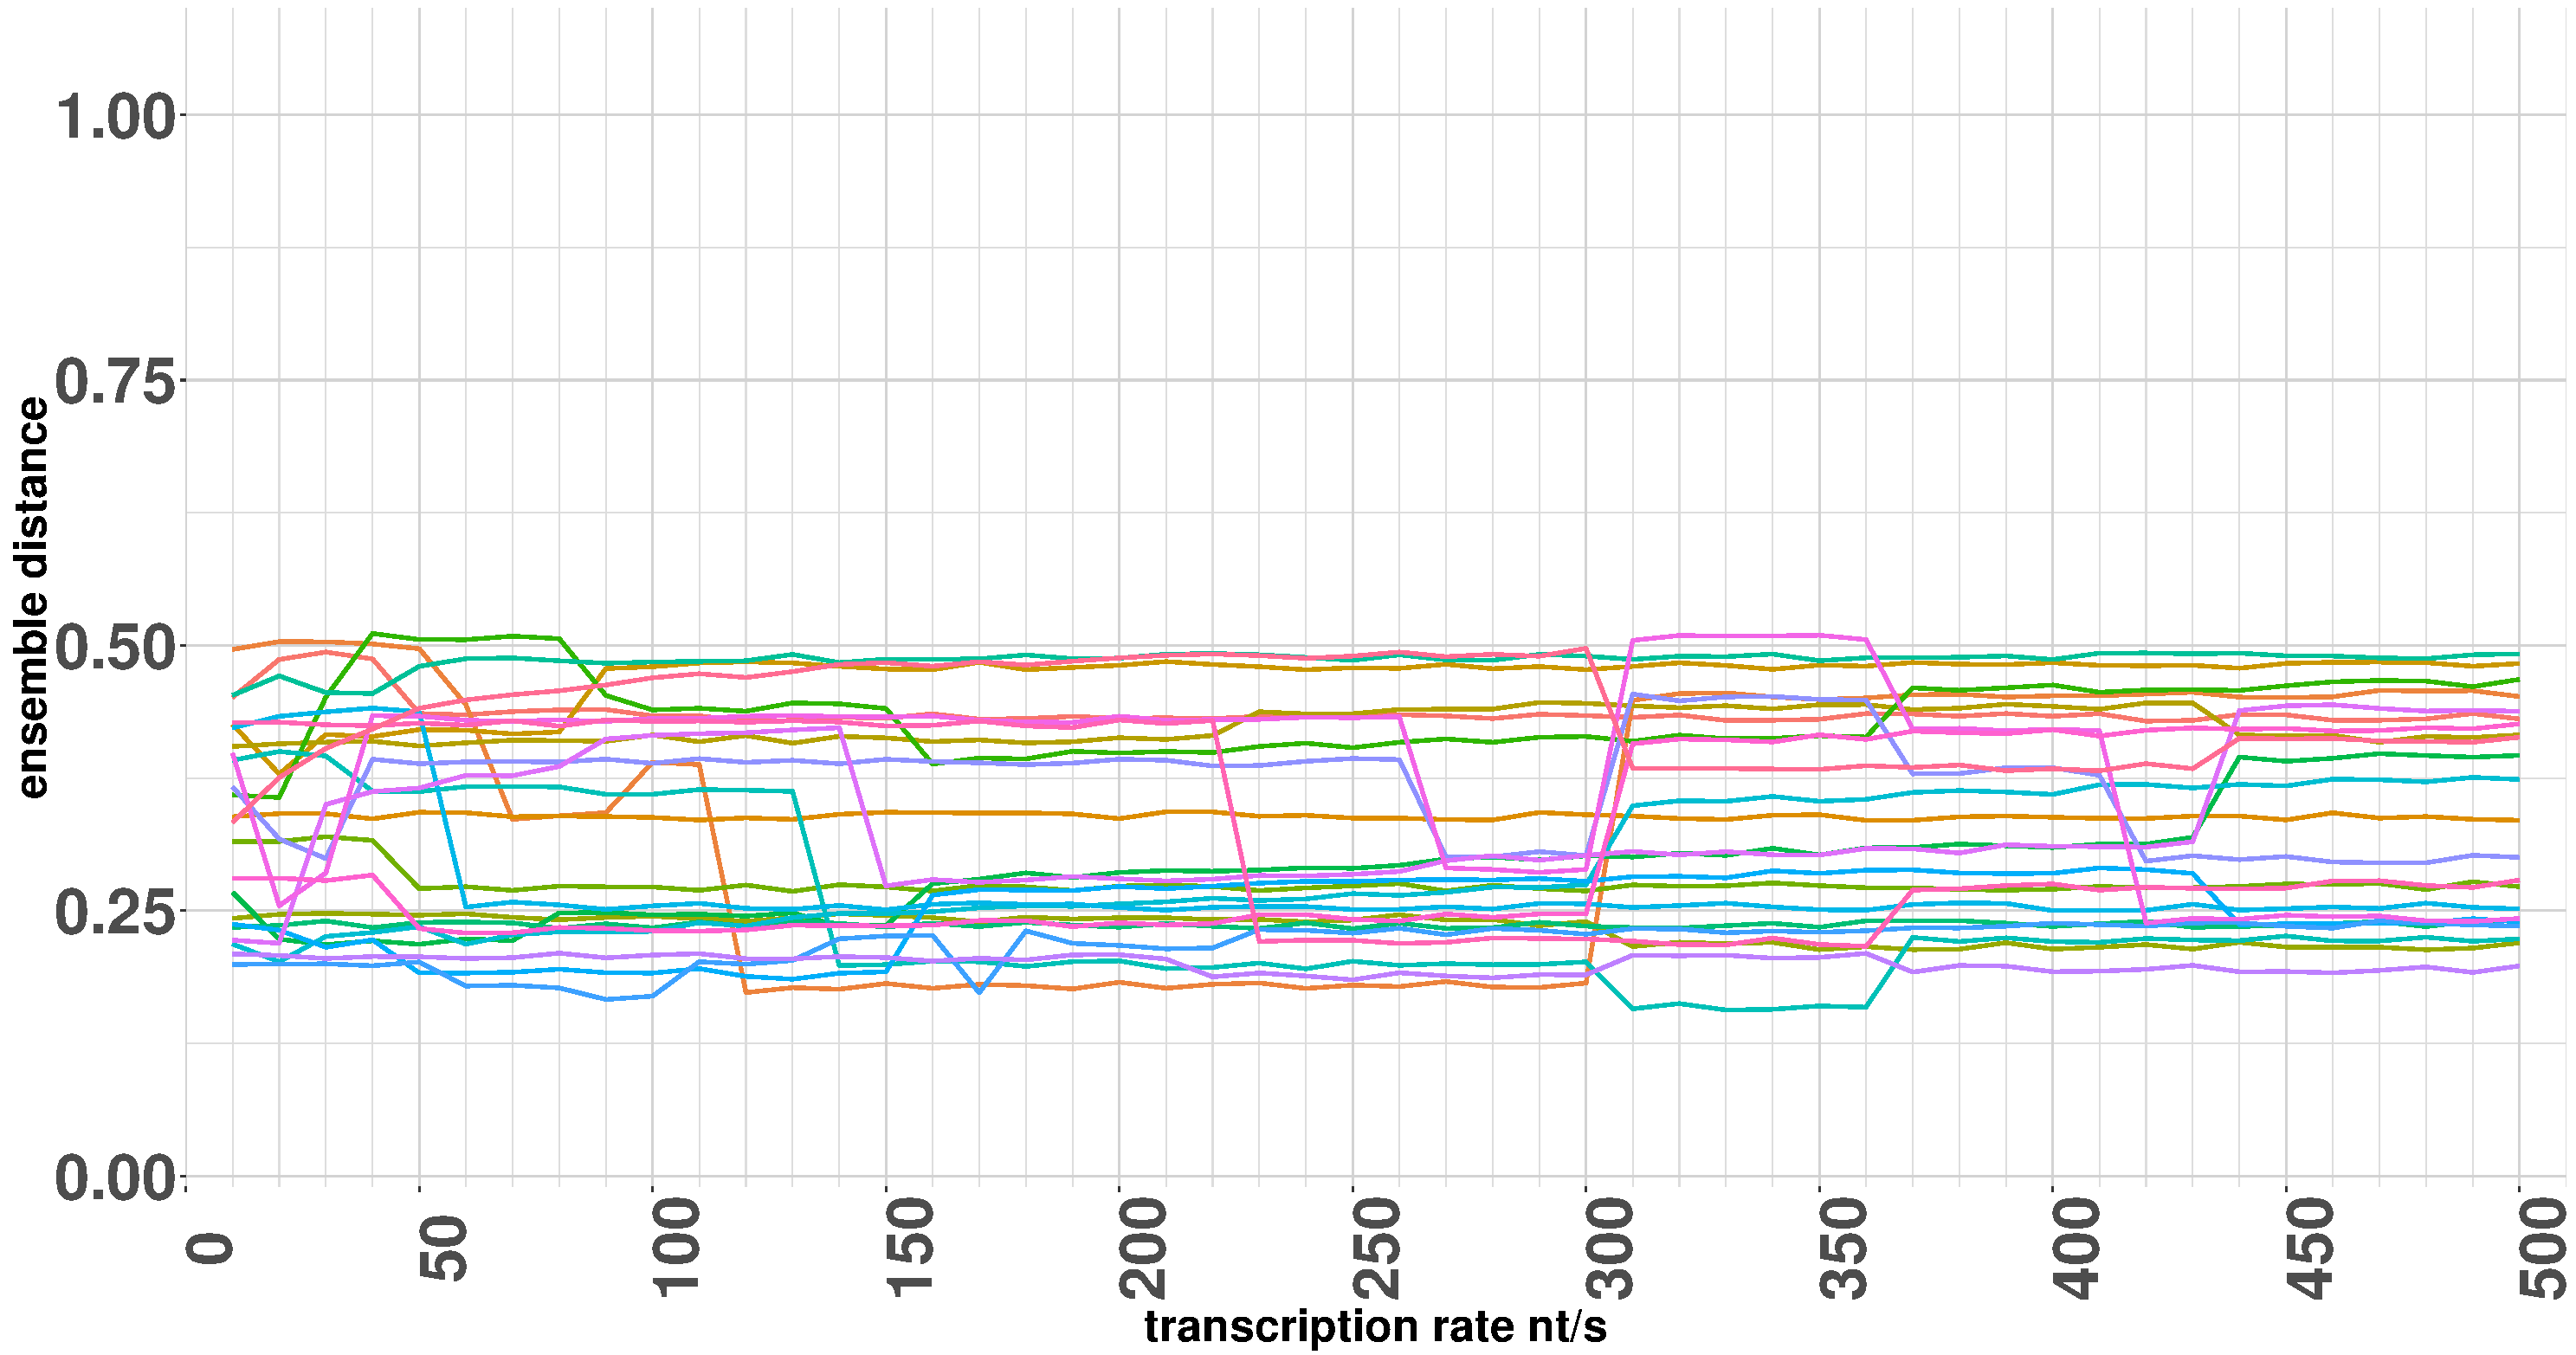
\includegraphics[width=0.9\textwidth]{./pictures/ensembleDistance/ensembleDistance_alternative1.pdf}\\
(b) \texttt{trpL} terminator \\
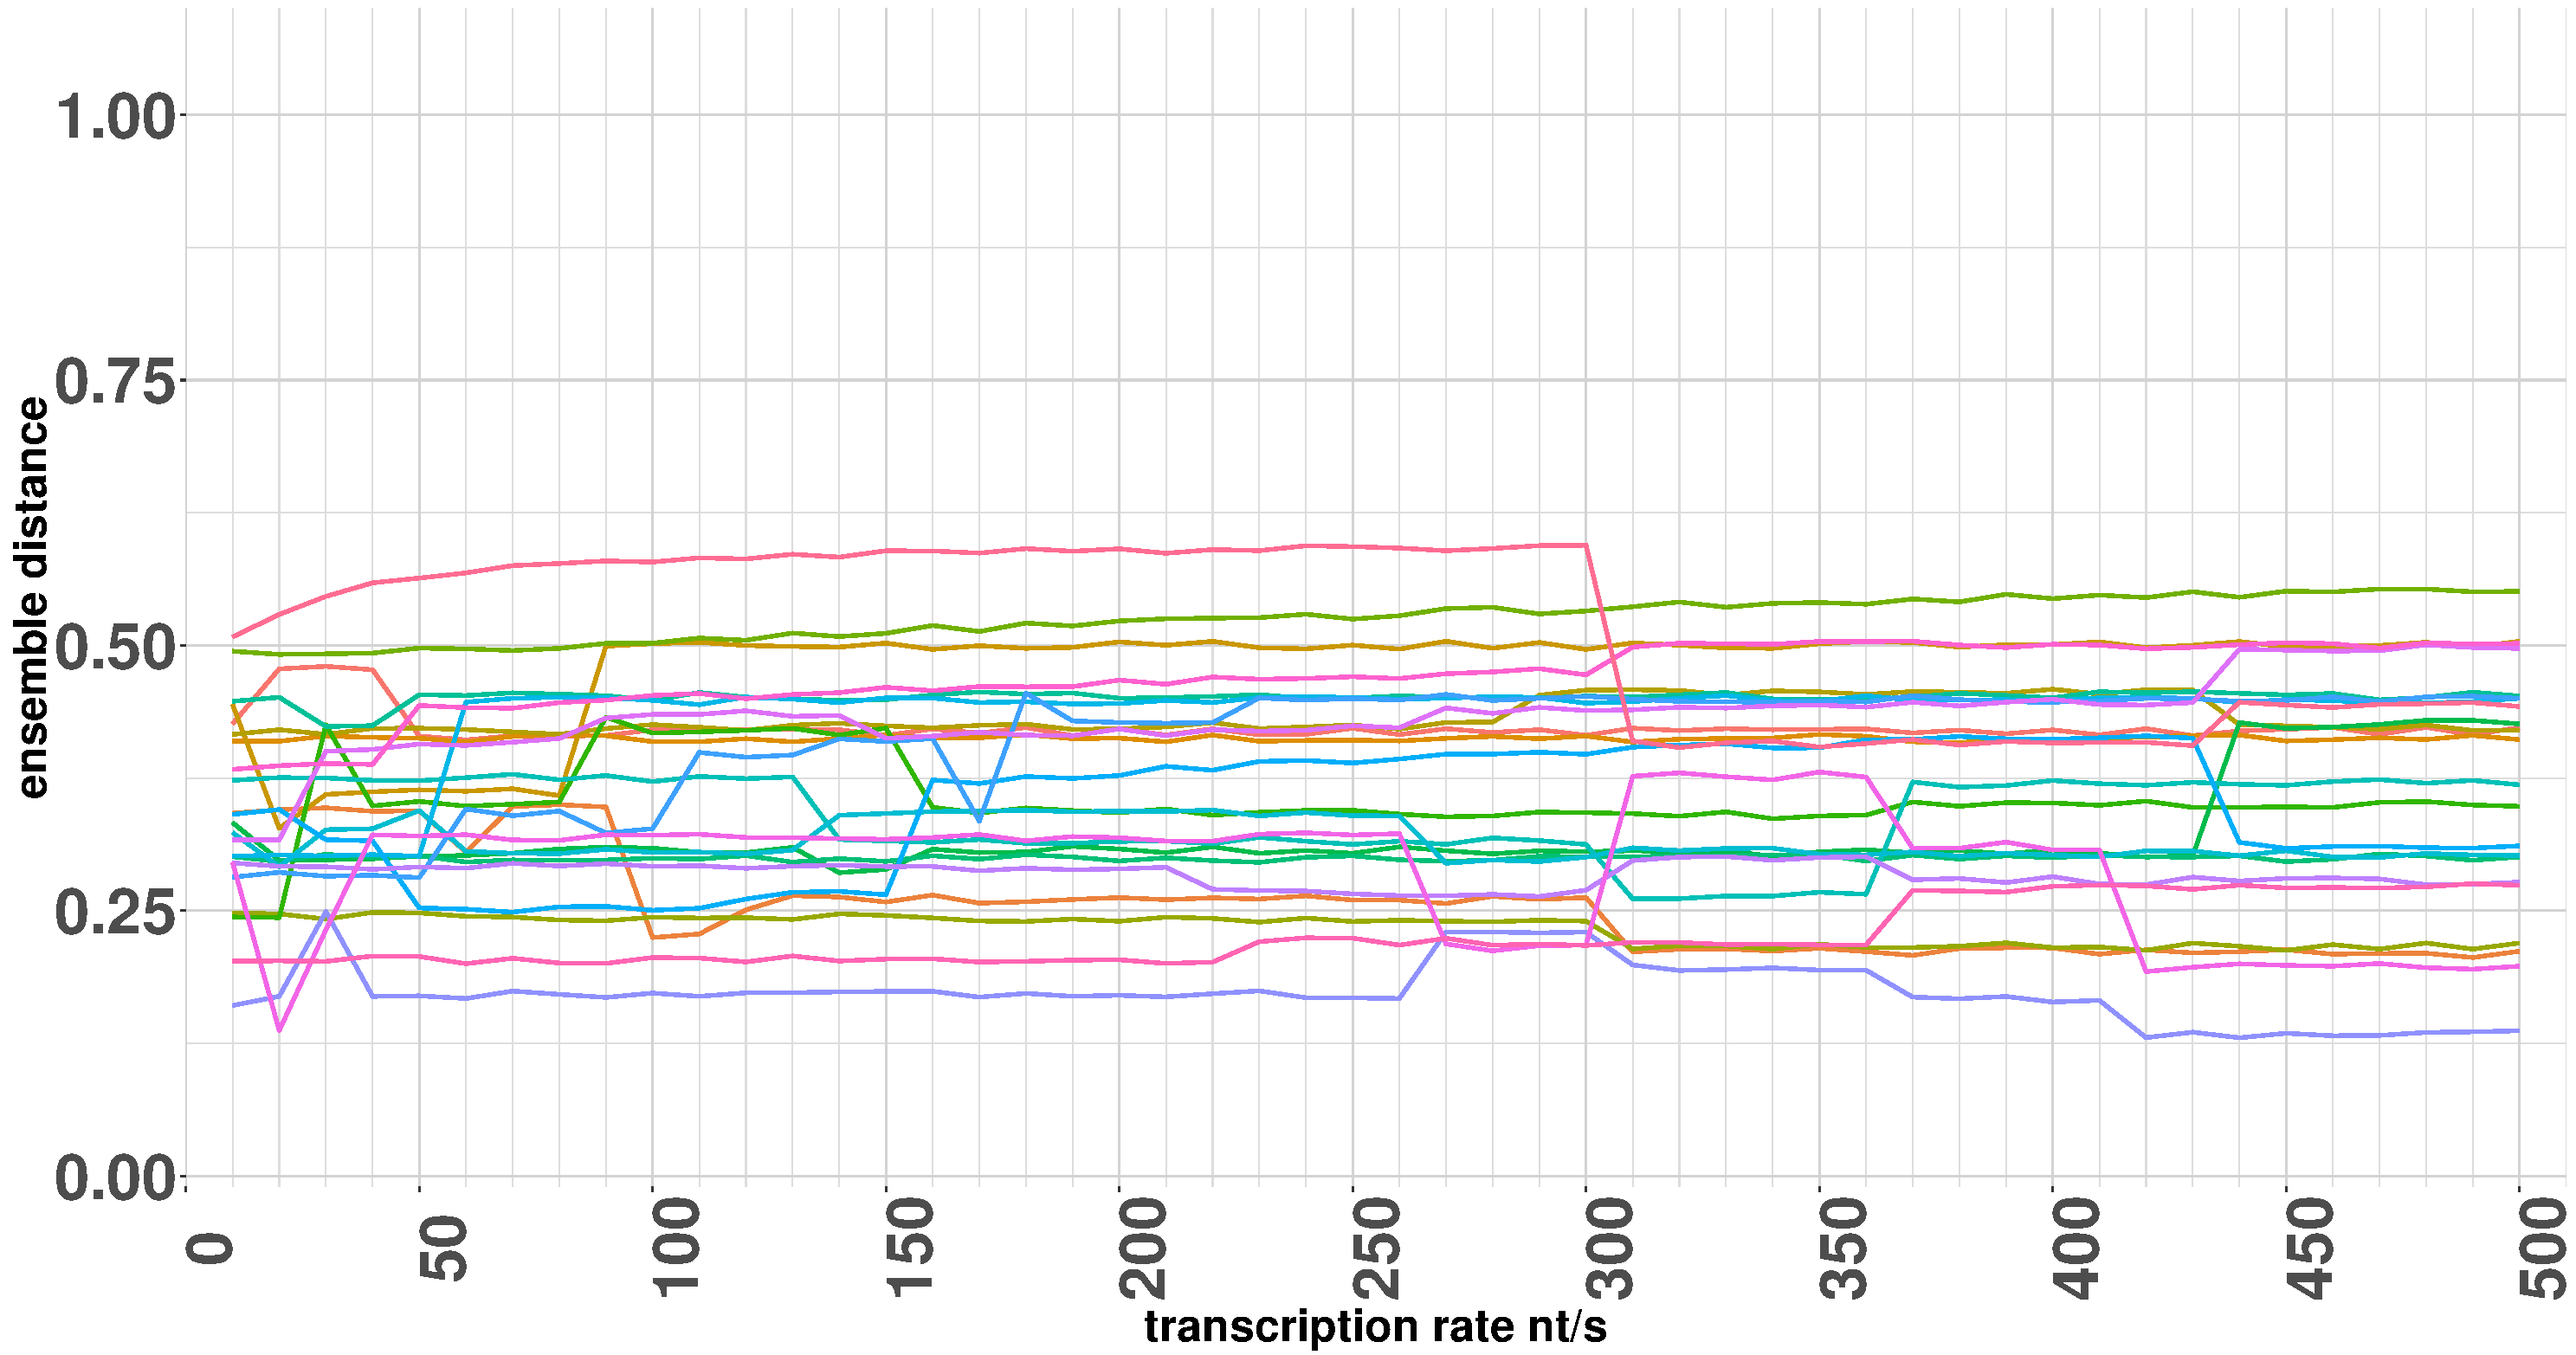
\includegraphics[width=0.9\textwidth]{./pictures/ensembleDistance/ensembleDistance_alternative2.pdf}\\
\end{tabular}
\caption{{\bf Ensemble distance of \texttt{trpL} family}
\texttt{findpath} and dangle option 2 were used.
(a) distance to antiterminator reference structure.
(b) distance to terminator reference structure.
}
\label{fig:ensembleDistanceTRP}
\end{figure}	
					
\begin{figure}
\begin{tabular}{l}
(a) \texttt{RNaseP} functional \\
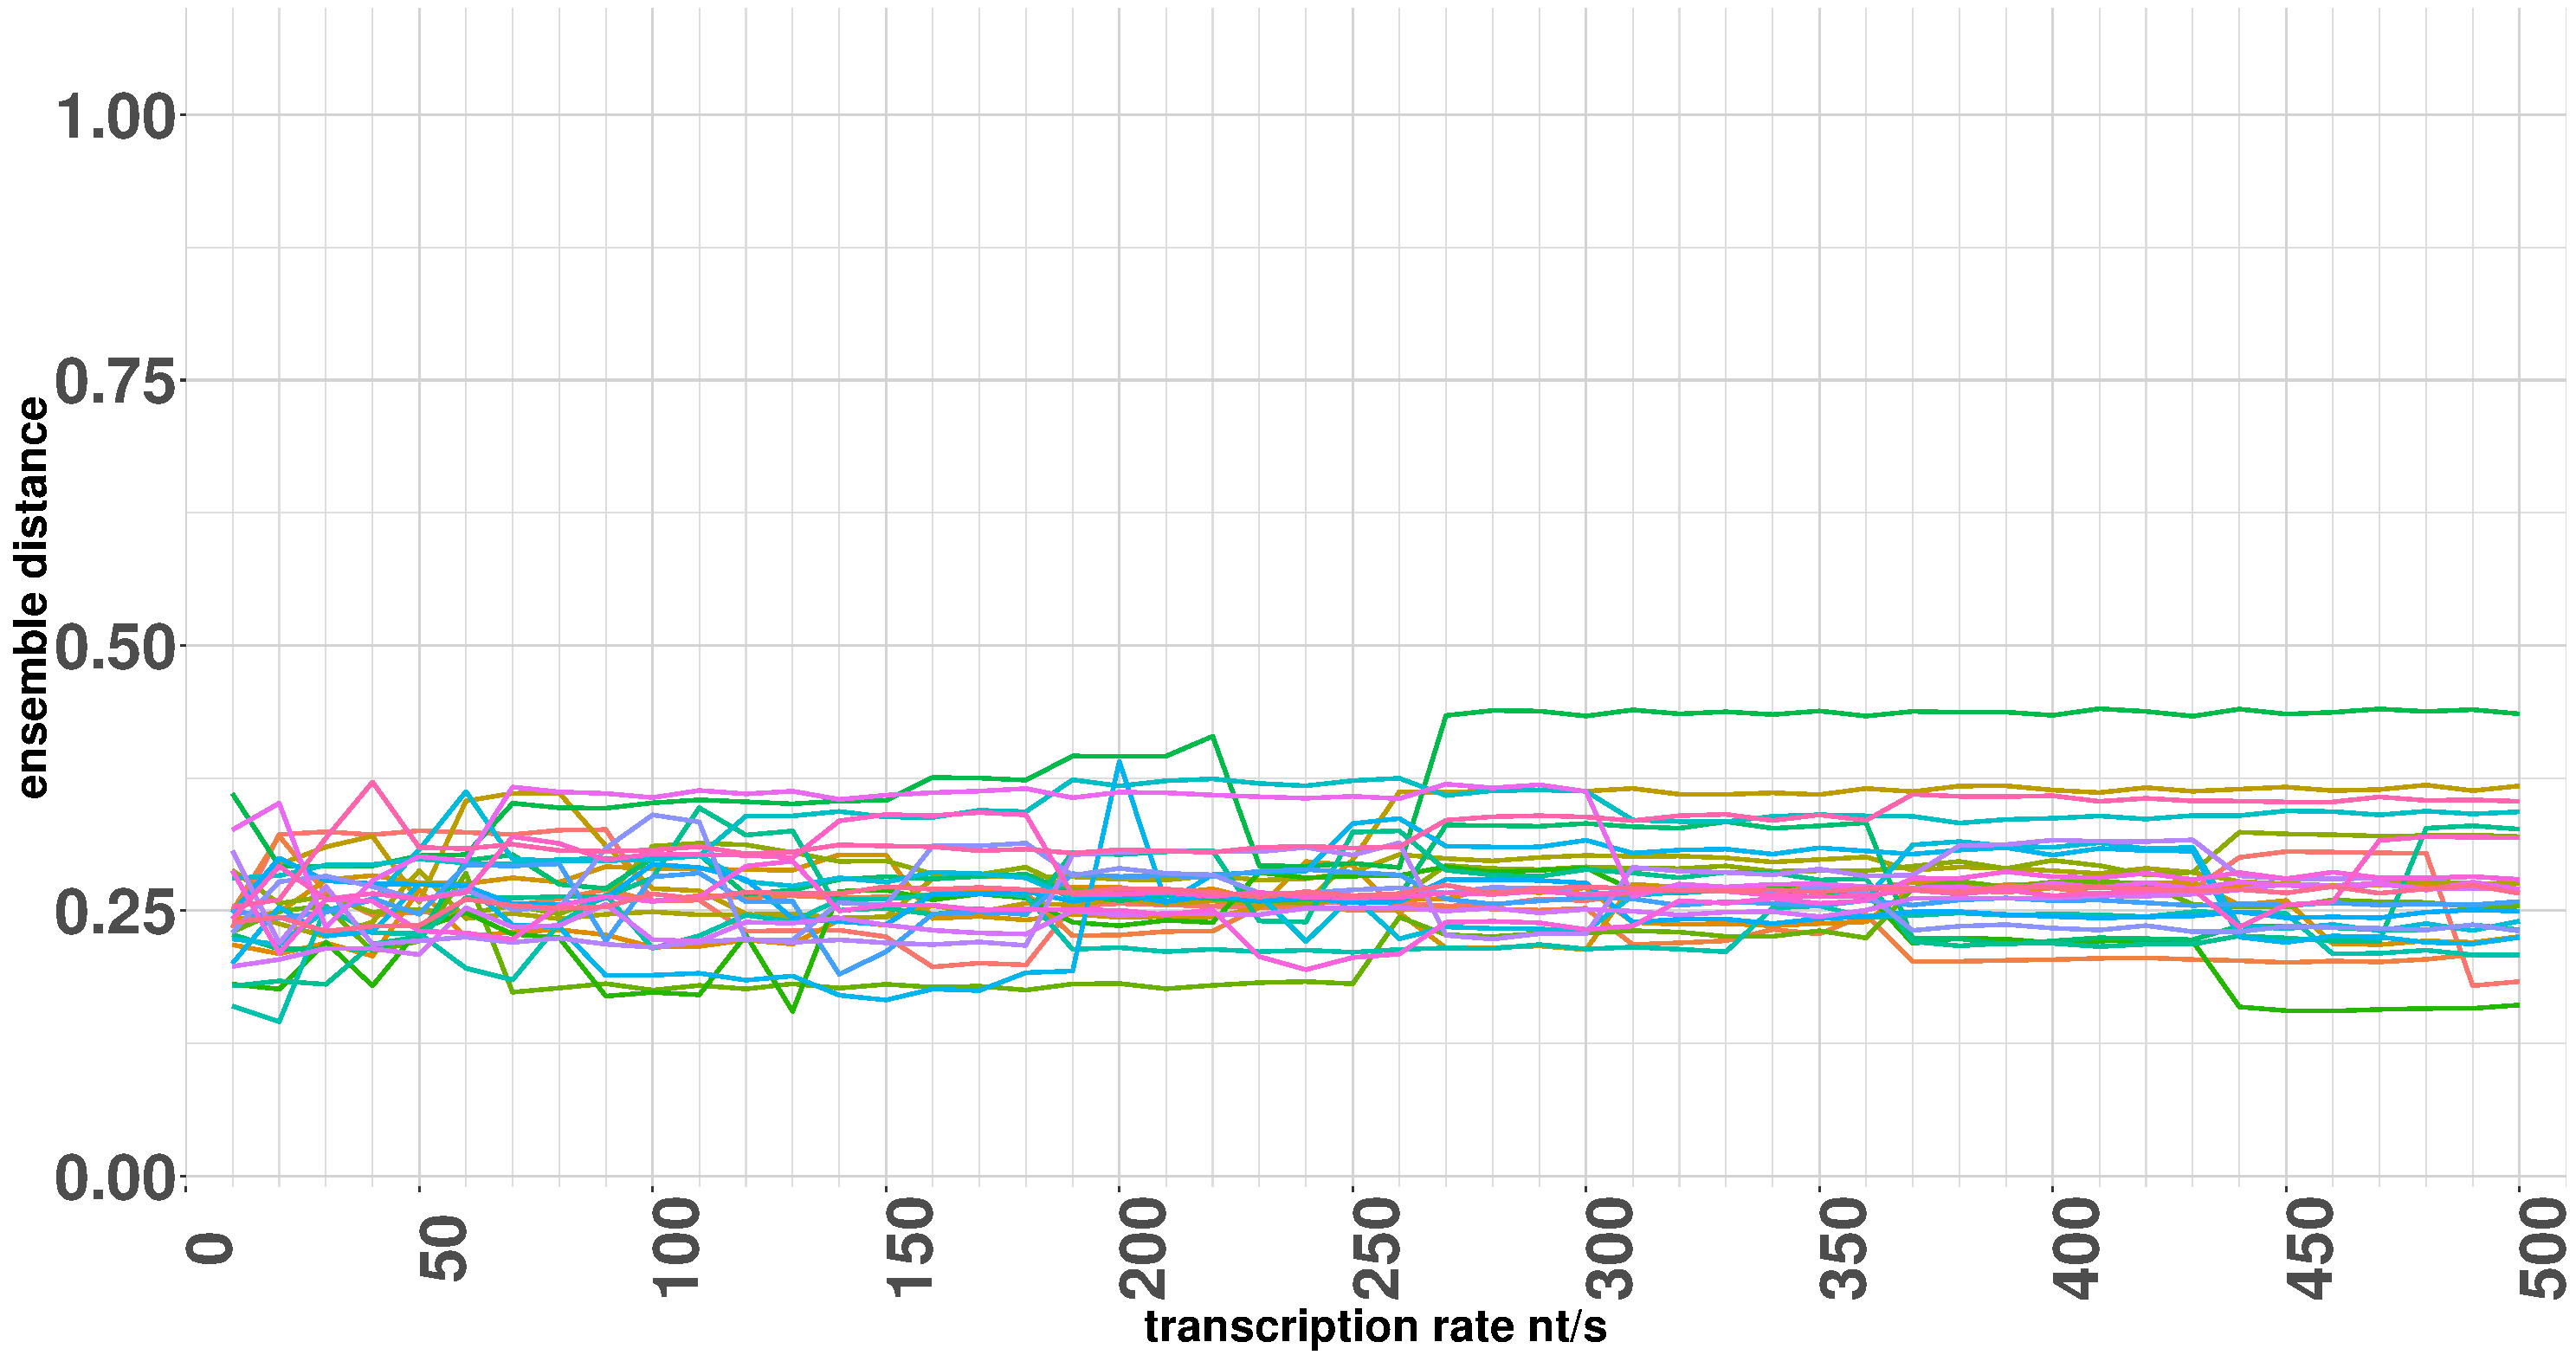
\includegraphics[width=0.9\textwidth]{./pictures/ensembleDistance/ensembleDistance_RNAseP.pdf}\\
\end{tabular}
\caption{{\bf Ensemble distance of \texttt{RNaseP} family}
\texttt{findpath} and dangle option 2 were used.
(a) distance to \texttt{RNaseP} functional reference structure. 
}
\label{fig:ensembleDistanceRNAseP}
\end{figure}
	
	

\FloatBarrier				

\chapter{Discussion}


After detailed parameter space tests and statistical analysis of the
results, I found out, that \texttt{Kinwalker} parameters, especially
transcriptions rates and pathfinding algorithms, have an impact
on co-transcriptional folding events. I divided this chapter into the following
sections: (i) the scores to highlight specific outcomes, restrictions or
improvements and (ii) into 2 biological observations I made from the data
created, one dealing with similar trajectory behavior of some \texttt{SRP} sequences
and the other one with the tryptophan operon.

\section{sequence similarity and SCI}


%\texttt{SRP}:
The \texttt{SRP} RNA is able to form the functional structure, as well as an intermediate transient structure.
The predicted consensus structure of the \texttt{SRP} family only shows base-pairs and loops of the functional structure (fig.~\ref{fig:sequence_similarity} a).
Furthermore, \texttt{SRP} has a high structure conservation (SCI of 0.8379), with a lot of compensatory mutations. Having only a sequence similarity of 0.682 \%, \texttt{SRP} has definitely evolved towards its functional structure. 

%trpL:
\texttt{trpL} RNA folds into two mutually exclusive functional structures: the
antiterminator loop and the terminator loop, both necessary for gene
expression regulation. The predicted consensus structure for the \texttt{trpL} RNA
is showing the functional terminator hairpin loop (fig.~\ref{fig:sequence_similarity} b). The other loop found
upstream of the terminator hairpin could be interpreted as the
antiterminator hairpin, although the predicted hairpin is too short. As the
color code indicates (red base-pairs), the terminator hairpin has nearly no
structure conservation through compensatory mutations but rather sequence
conservation at this hairpin.

%RNaseP:
\texttt{RNaseP} has the highest sequence similarity with 0.891 \%, but a lower SCI
(0.7854) than trpL, indicating that the MFE structures of the individual sequences of the
alignment differ slightly from the consensus structure (fig.~\ref{fig:sequence_similarity} c).
The predicted
consensus structure and the \texttt{RNaseP} functional structure have few loops and
base-pairs in common. This could be the case because the functional RNaseP
structure forms pseudo-knots which cannot be predicted by the
\texttt{RNAalifold} methods used to calculate the consensus structure.


\section{base-pair diversity}

When investigating the base-pair diversity for all three RNA families, I
expected to find lower diversity when using base-pair time-scoring than
without considering time. This result was indeed found in all three
families.
%and is due to
%the fact that inserting lifetime of a base-pair is of course a much better
%scoring function for base-pair diversity than without the time-scoring.
In general, including time into the score leads to a more constant diversity
throughout all parameters and families, due to the fact that short-living
base-pairs are weighted accordingly to their existence in the folding
simulation and are not scored as high as long living base-pairs.

\texttt{SRP} reference RNA shows a diversity decrease with both options (time
dependent and independent) at transcription rate ranging from 260 to 300
nt/s if \texttt{findpath} with dangle option 2 was used
(fig.~\ref{fig:base-pair diversity}).
The first possibility would be the direct folding into its MFE structure
without detours (which would lead to few different 
base-pairs). Another possible explanation could be the instant folding into
a local favorable energy minimum, where it becomes trapped and stays for
the entire simulation. Here \texttt{SRP} reference sequence is folding directly into the MFE structure at transcripiton rates ranging from 260 to 300 nt/s and is folding into a local energy minimum outside this range.
Another such noteworthy decrease happens at transcriptions rates of 20 nt/s with
\texttt{Morgan$-$Higgs} algorithm and dangle option $0$. 

One big similarity found in the \texttt{SRP} and \texttt{RNaseP} families, is the increase in
diversity variations at low transcription rates (fig.~\ref{fig:base-pair
  diversity alignments}). Higher transcription rates (i.e. over 120 nt/s)
result in more compact co-transcriptional folding patterns. On the
other hand, the base-pair diversity for \texttt{trpL} is rather constant over different
transcription rates.

The base-pair diversity score is useful to describe how much a sequence
refolds during transcription. However, it is not able to cover two
important questions:

\begin{enumerate}
\item Base-pairs that appear later during transcription have per definition
  a shorter life-time than those further downstream towards the 5' end.
  Although a time factor is inserted into the formula, this problem is not
  addressed here. For example: a base-pair with bases at position 2 and 7
  (start at 5' end) has a theoretically longer time to exist than a
  base-pair with a base at position 200 (start at 5'), simple because of
  the fact, that it was earlier transcribed. The later formed base-pair
  could contribute significantly more stability into the structure, but is
  never considered as important.

\item Calculation of the lifetime of base-pair $(i,j)$ ($\Delta Time_{ij}$) from
  \texttt{Kinwalker} output. A \texttt{Kinwalker} output does not show every
  substructure formed after each newly transcribed base. The determination
  of the exact existence time of a base-pair is therefore not possible.
  Figure:\ref{fig:fig_bp_lifetime_calculations} shows two lines of
  \texttt{Kinwalker} output. Base-pair (2,21) would get an lifetime of
  0.40055 ($5.5014-5.10085$), because base-pair (2,21) does not exist any
  more in the next line (next structure). During transformation from the
  previous structure to the new structure a total of 4 bases are added to
  the growing RNA chain. It remains unknown whether the base-pair (2,21)
  was dissolved during transcription of the first new base, or during the
  last, or in between. Because there is no exact way of telling how long
  this one base-pair existed, I simply assume in my calculations, that a
  base-pair exists until a new structure without this particular base-pair
  is calculated by \texttt{Kinwalker}. Therefore, base-pair (2,21) gets a
  lifetime of 0.4 when calculating base-pair diversity with time normalization.
\end{enumerate} 
			
\begin{figure}[ht] 
\centering
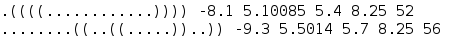
\includegraphics[width=0.7\textwidth]{./pictures/TimeCalculation.png}
\caption{base-pair lifetime calculation}
\label{fig:fig_bp_lifetime_calculations}
\end{figure}		


 
\section{ensemble diversity}
Base-pair diversity was further improved by introducing the ensemble diversity score (equation:~\ref{eq:ensemble diversity
}).
%\todo{here we have the probability of observing a bp only if the respective sequence exists already? ronny.}
%Here, I consider that a the hypothetical maximal lifespan of a bp depends
%on the position within the sequence and this the time it was transcribed.

By comparing the ensemble diversity score for the \texttt{SRP} reference sequence
with the base-pair diversity score, an interesting result occurs. The same
transcription rates have outliers, but invers ones. The area of 260 to 300 nt/s
for \texttt{findpath} and dangle option 2, shows a base-pair diversity
decrease but also an ensemble diversity increase (fig.~\ref{fig:comparison_SRPensemblediversity_bpdiversity}). After
manually analyzing the \texttt{Kinwalker} output files, I came to
following conclusion. With transcription rates of 260 to 300 nt/s and
\texttt{findpath}/dangle 2, \texttt{SRP} reference sequence folds relatively early into
the MFE structure. During he first half of transcription, it creates non
MFE base-pairs at the 5' end similar to the ones experimentally identified
as transient structure. These transient hairpins seem to prevent the
sequence from forming stable intermediate structures and thus falling into a folding trap.
This scenario leads to the high ensemble
diversity in this area. With every other transcription rate, the sequence
falls into a folding trap, refolding into the MFE only after a large amount
of time. The time needed precedes the life-time of an RNA molecule, and is
therefore only theoretically possible.
Taking these results together, I suggest to use transcription rates of
260 to 300 nt/s when analysing \texttt{SRP} RNA with \texttt{Kinwalker}.

\begin{figure}
\begin{tabular}{l}
X01074.1/170-275 base-pair diversity\\
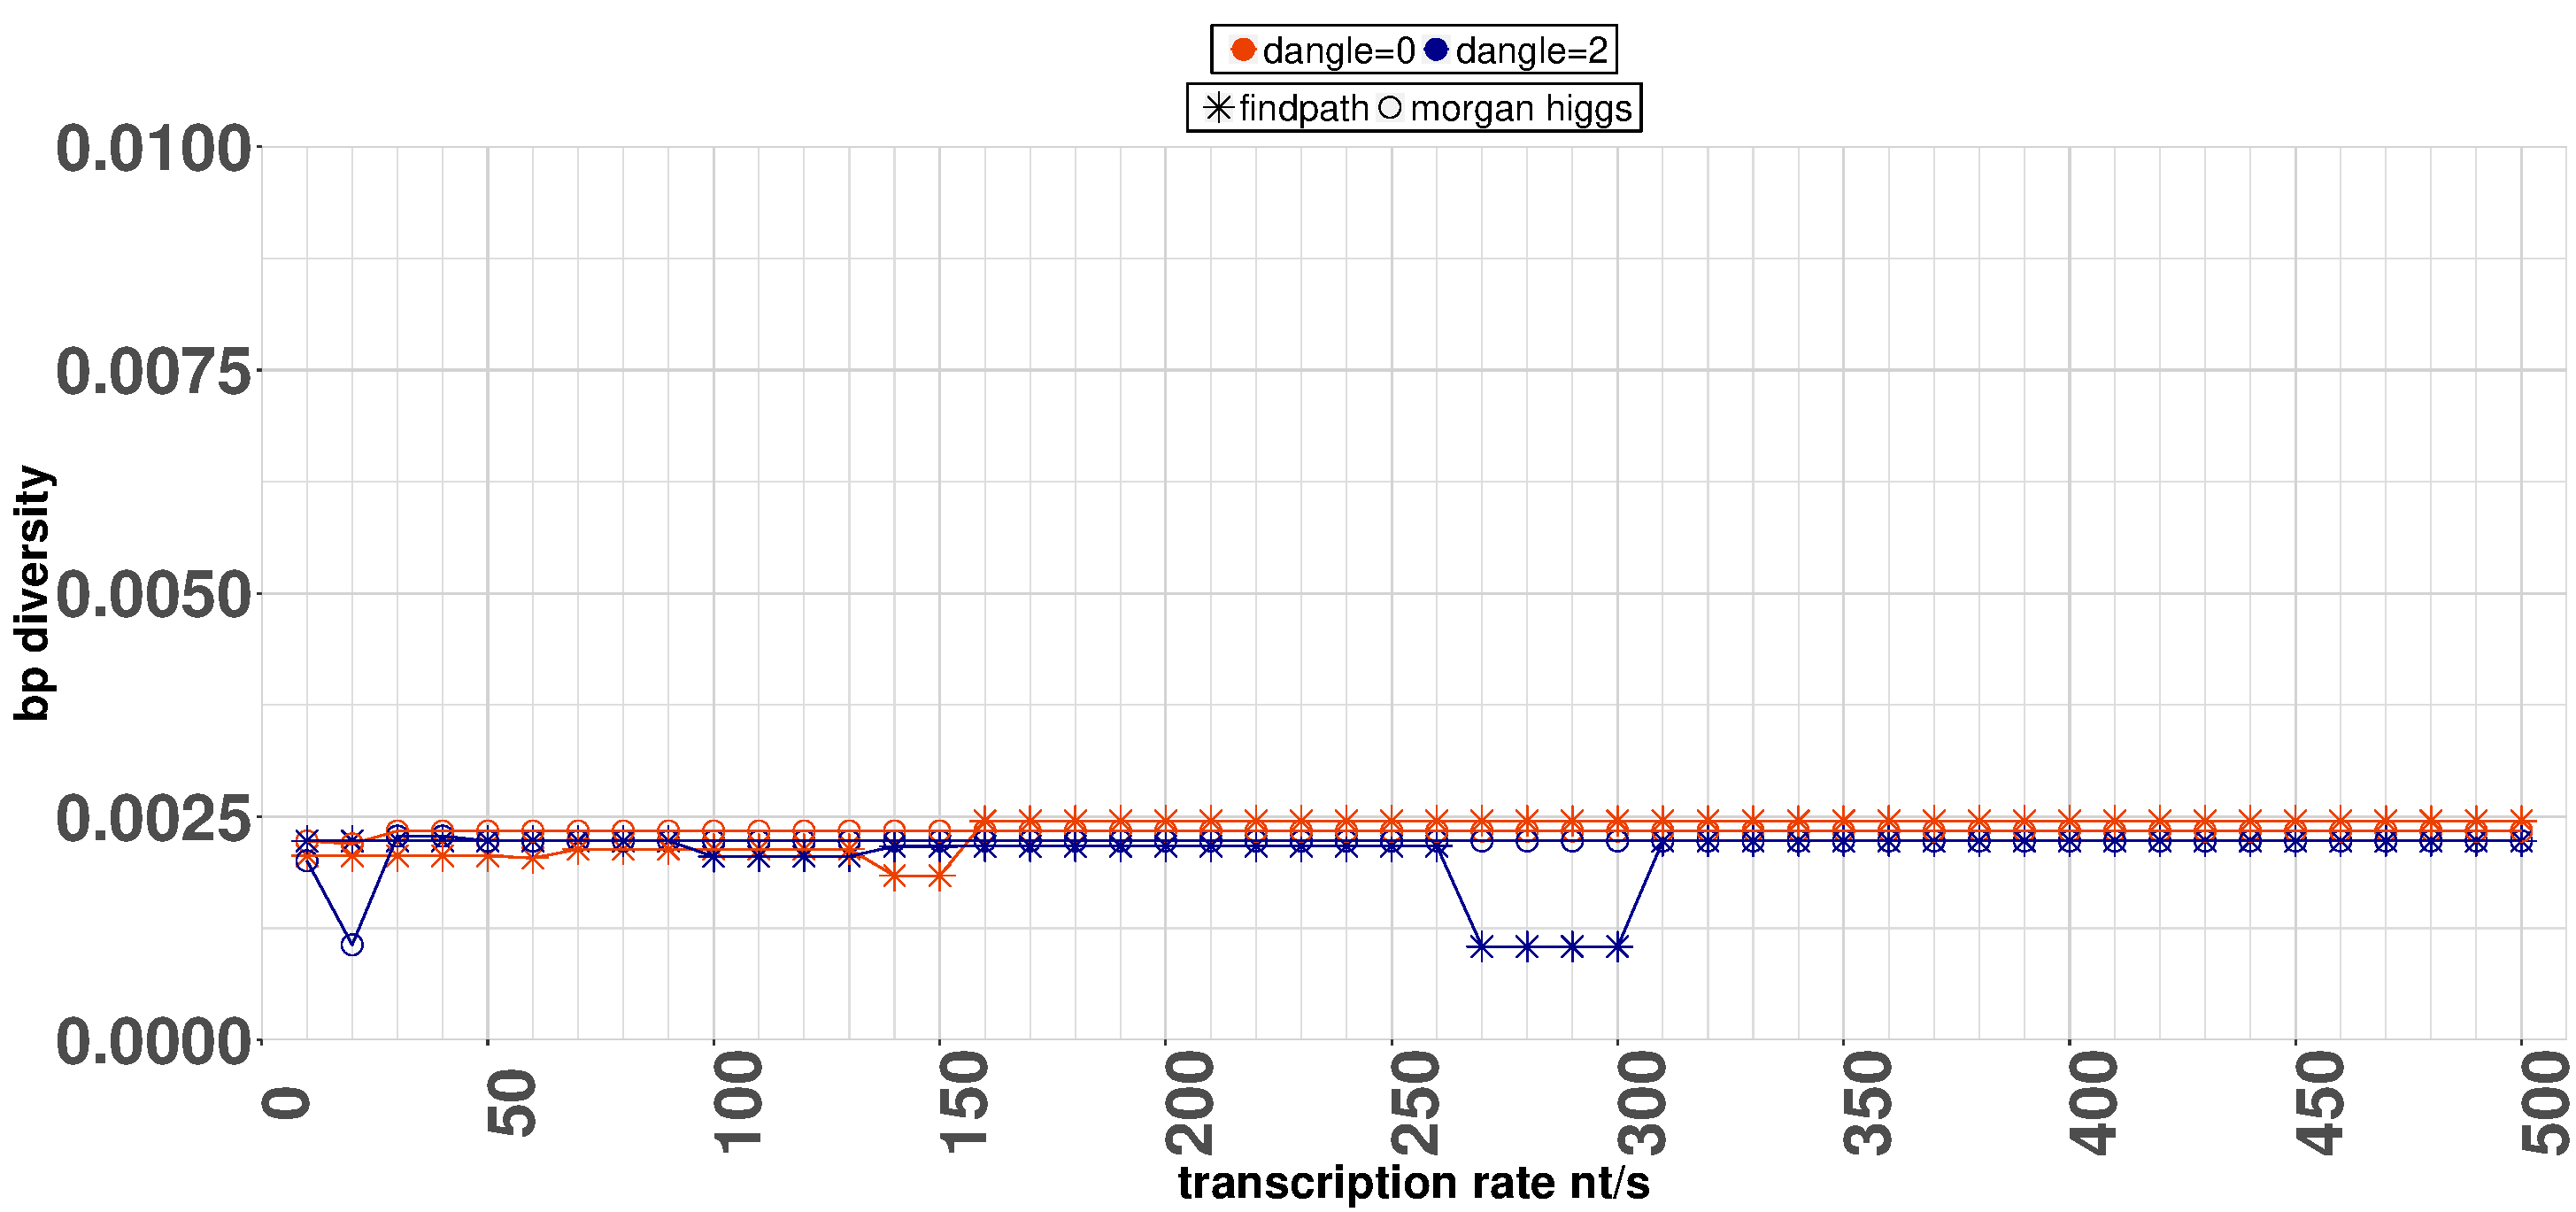
\includegraphics[width=0.9\textwidth]{./pictures/basePairDiversity/TimeDepended/SRPWithTime.pdf}\\
X01074.1/170-275 ensemble diversity\\
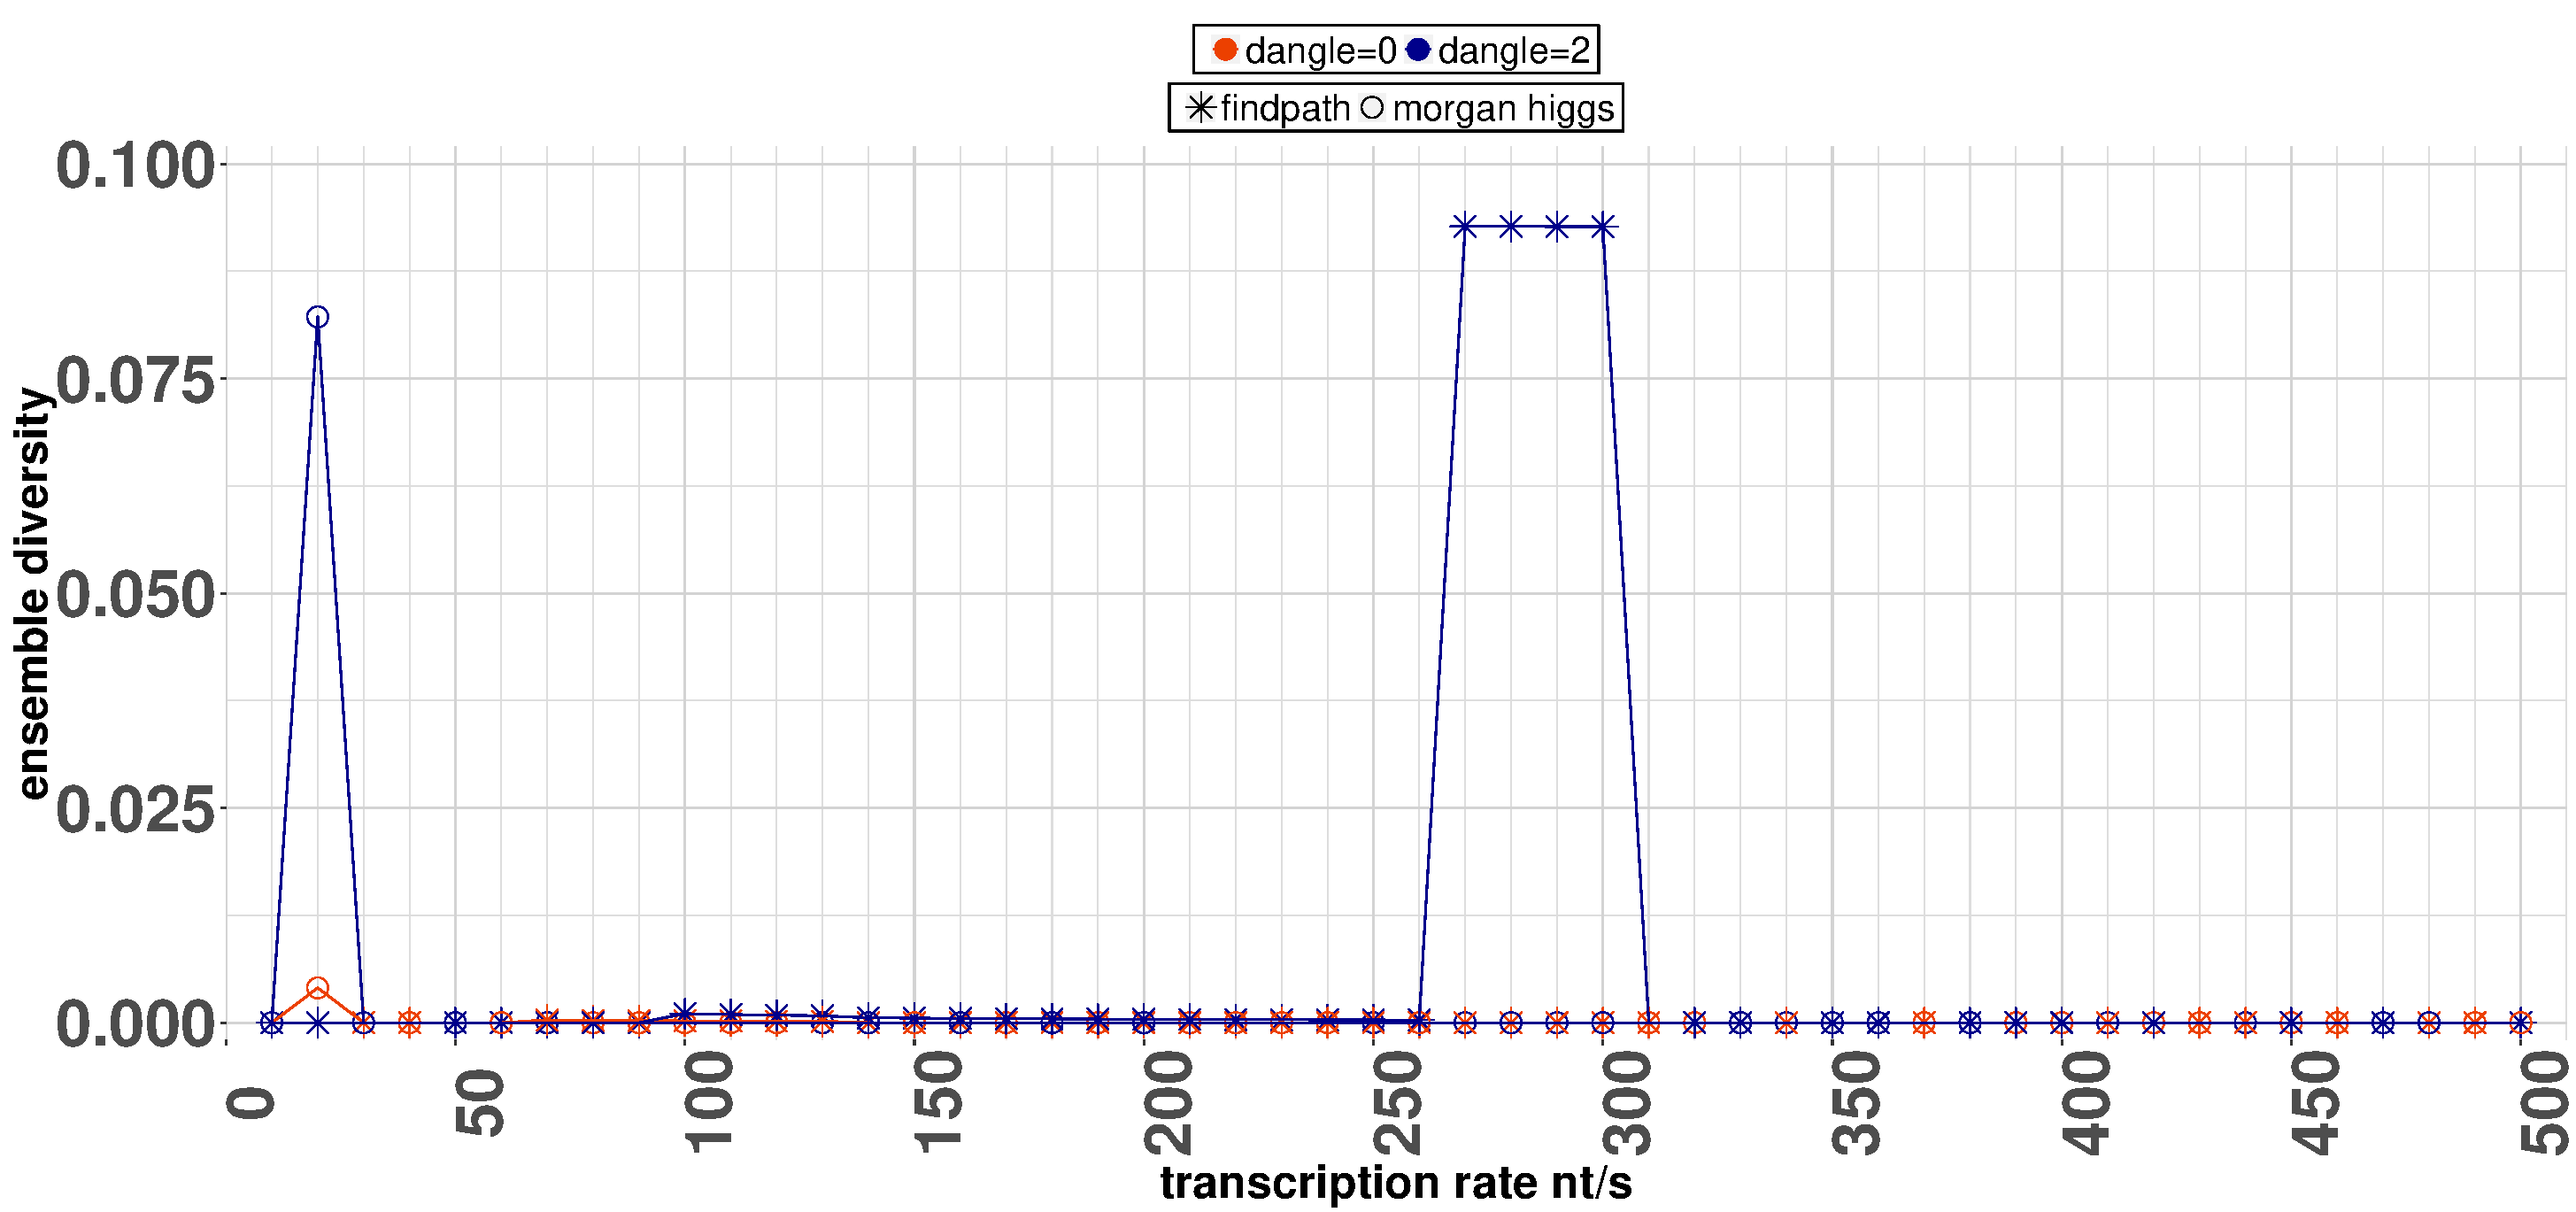
\includegraphics[width=0.9\textwidth]{./pictures/ensembleDiversity/SRP2510.pdf}\\
\end{tabular}
\caption{{\bf comparison of base-pair diversity and ensemble diversity for \texttt{SRP} reference sequence.}
Transcription rates of 260 to 300 nt/s with \texttt{findpath} algorithm and dangle option 2, show a base-pair diversity decrease but also an ensemble diversity increase.}
\label{fig:comparison_SRPensemblediversity_bpdiversity}
\end{figure}
\FloatBarrier\


%ensemble diversity Time periods
The ensemble diversity score was further improved by using different time periods within the ensemble diversity
calculations.
The idea of using different time periods was to determine at what time during or after transcription,
diversity variations occur. Due to the fact that the time periods were
chosen various times higher than the normal transcription time, the time
span between transcription end and successfully folding into the MFE can be
further analyzed.  If diversity increase happens with $10
\times$transcription time but not with 2/5 transcription times, refolding into the MFE starts long after transcription has
finished (i.e. between
$5 \times$transcription time and $10 \times$transcription time). If the
diversity stays the same with $2/5/10 \times$transcription times, than
refolding happens shortly after finishing transcription.  Such a late
refolding from a folding trap to the MFE structure can be seen for \texttt{RNaseP} (fig.~\ref{fig:ensemble_diversity_AE005174.2}). Only if the time until $10
\times$transcription rate was analyzed, a diversity change can be seen with
\texttt{findpath} and dangle option $0$. I suggest, that such late changes
are not possibly in reality, because refolding into the MFE would take to
long.


\section{ensemble distance}
The idea of using the ensemble distance is to determine whether the base-pairs of an intermediate
structure are present in the the folding trajectory of a sequence.

One big similarity that is apparent in every family, is the increased
distance changes at lower transcription rates. This behavior might occur,
because with lower transcription rates, RNA sequences have more time to
form secondary structures. If the next base is transcribed too fast,
another structure (containing the new base) could be energetically favored,
and the prior structure could never form.  
Note that there is no evidence
that the used reference structures have to be part of the folding
trajectory of every alignment sequence. The reference structure is an
experimentally defined structure, whereby the corresponding sequence is
part of the chosen alignment. Deviations between the reference sequence and
another alignment sequence could be so high, that the reference structure
can never form.

\section{attenuation of trp operon}
Here I investigated the attenuation behavior of the \texttt{trpL} transcript upstream of the trp operon, especially the ensemble distance to the terminator and anti-terminator structure of trpL.
As explained before, the attenuation and therefore regulation of the trp operon is correlated with the formation of secondary structures (i.e. 2 different hairpins) on the trp leader transcript (trpL) \cite{Yanofsky1977},\cite{Oxender1979}.


The most important feature of regulation via attenuation, is the formation of the terminator hairpin (i.e. 3-4), because this will occupy area 3, and therefore the stalling hairpin (2-3) cannot form. 
%Although alternative structure 2 and the described terminator hairpin form another upstream hairpin prior to the real 3-4 terminator hairpin, this upstream structure varies in different publications and I consider it as not not important for my studies. 
For the following analysis, I defined only the small 3-4 hairpin at the 5 prime end as the terminator structure. This terminator hairpin consists of strong G-C bonds and a slippery multiple U sequence, for detaching the RNA strand from the polymerase, if transcription stop should be achieved.

I analyzed the ensemble distances of every \texttt{trpL} sequence to the antiterminator hairpin (fig.~\ref{fig:ensembleDistanceTRP} a) and to the terminator hairpin (fig.~\ref{fig:ensembleDistanceTRP} b) to determine influences of transcription rates.
I detected no significant influence of transcription rate to the formation of the terminator hairpin. Some sequences have a high ensemble distance to the terminator hairpin at low transcription rates, others on higher.
Simultaneously, I cannot detect any preferences to form the anti-terminator hairpin at specific transcription rates.




\section{SRP analysis}

A hint of evolutionary conservation of co-transcriptional folding can be
observed in figure: \ref{fig:SRPDecrease250_300}. The shown five sequences
result with a base-pair diversity decrease at the area of 270 to 300 nt/s.
Following sequences are affected: X01074.1/170-275,
CP001127.1/532559-532656, U00096.2/475680-475777, FM180568.1/436931-437028
and CP001138.1/505976-506073. It is noteworthy, that this sequences also
show the same behavior with other scores. After manually analyzing the
\texttt{Kinwalker} output files for this sequences and transcription rate
areas, I investigated, that inside this area these sequences are folding
into the MFE without detours, but are forming folding traps with
transcription rates outside this area. CP000058.1/2086711-2086808 was used
as a negative control and is always forming a folding trap as expected. For
these sequences, lower base-pair diversity leads to the direct folding into
their MFE structure. Furthermore all of these sequences are forming similar
folding trajectories in these specific area. To answer the question what
kind of structures are formed, the ensemble distance delivers interesting
results. The base-pair-diversity drop at 270 to 300 nt/s is also visible with
the ensemble distance scores for both reference structures, \texttt{SRP} transient
and \texttt{SRP} functional, as shown in figure:~\ref{fig:ensembleDistanceSRP}. I
conclude, that for these sequences, the \texttt{SRP} transient and \texttt{SRP} functional
structure are important intermediate structures, required to fold into
their MFE structures. Outside this transcription rate area, folding traps
occur, and therefore less base-pairs from transient and functional
structure can form.

Calculation of a phylogenetic tree for the \texttt{SRP} family (fig.~\ref{fig:SRP_PhyloTree} a) shows, that these sequences form a closed subgroup, which lead to further prove of co-transcriptional folding conservation. To convert the species names with sequence accession-numbers, table:~\ref{table:SRPAcessionToSpeciesName}, provided in the appendix, as well as figure:~\ref{fig:SRPSpeciesTree} can be used. Further investigation with the global multiple sequence alignment tool \texttt{RNAalifold} (fig.~\ref{fig:SRP_PhyloTree} b) shows, that these five sequences are basically the same and no compensatory mutations are visible. Therefore it is understandable that these sequences are forming identical folding trajectories. I conclude, that this sequence behavior is no evidence for co-transcriptional folding conservation but rather for evolutionary sequence conservation in \texttt{Enterobacteriaceae.} 

\begin{figure}
\begin{tabular}{l}

(a) \\
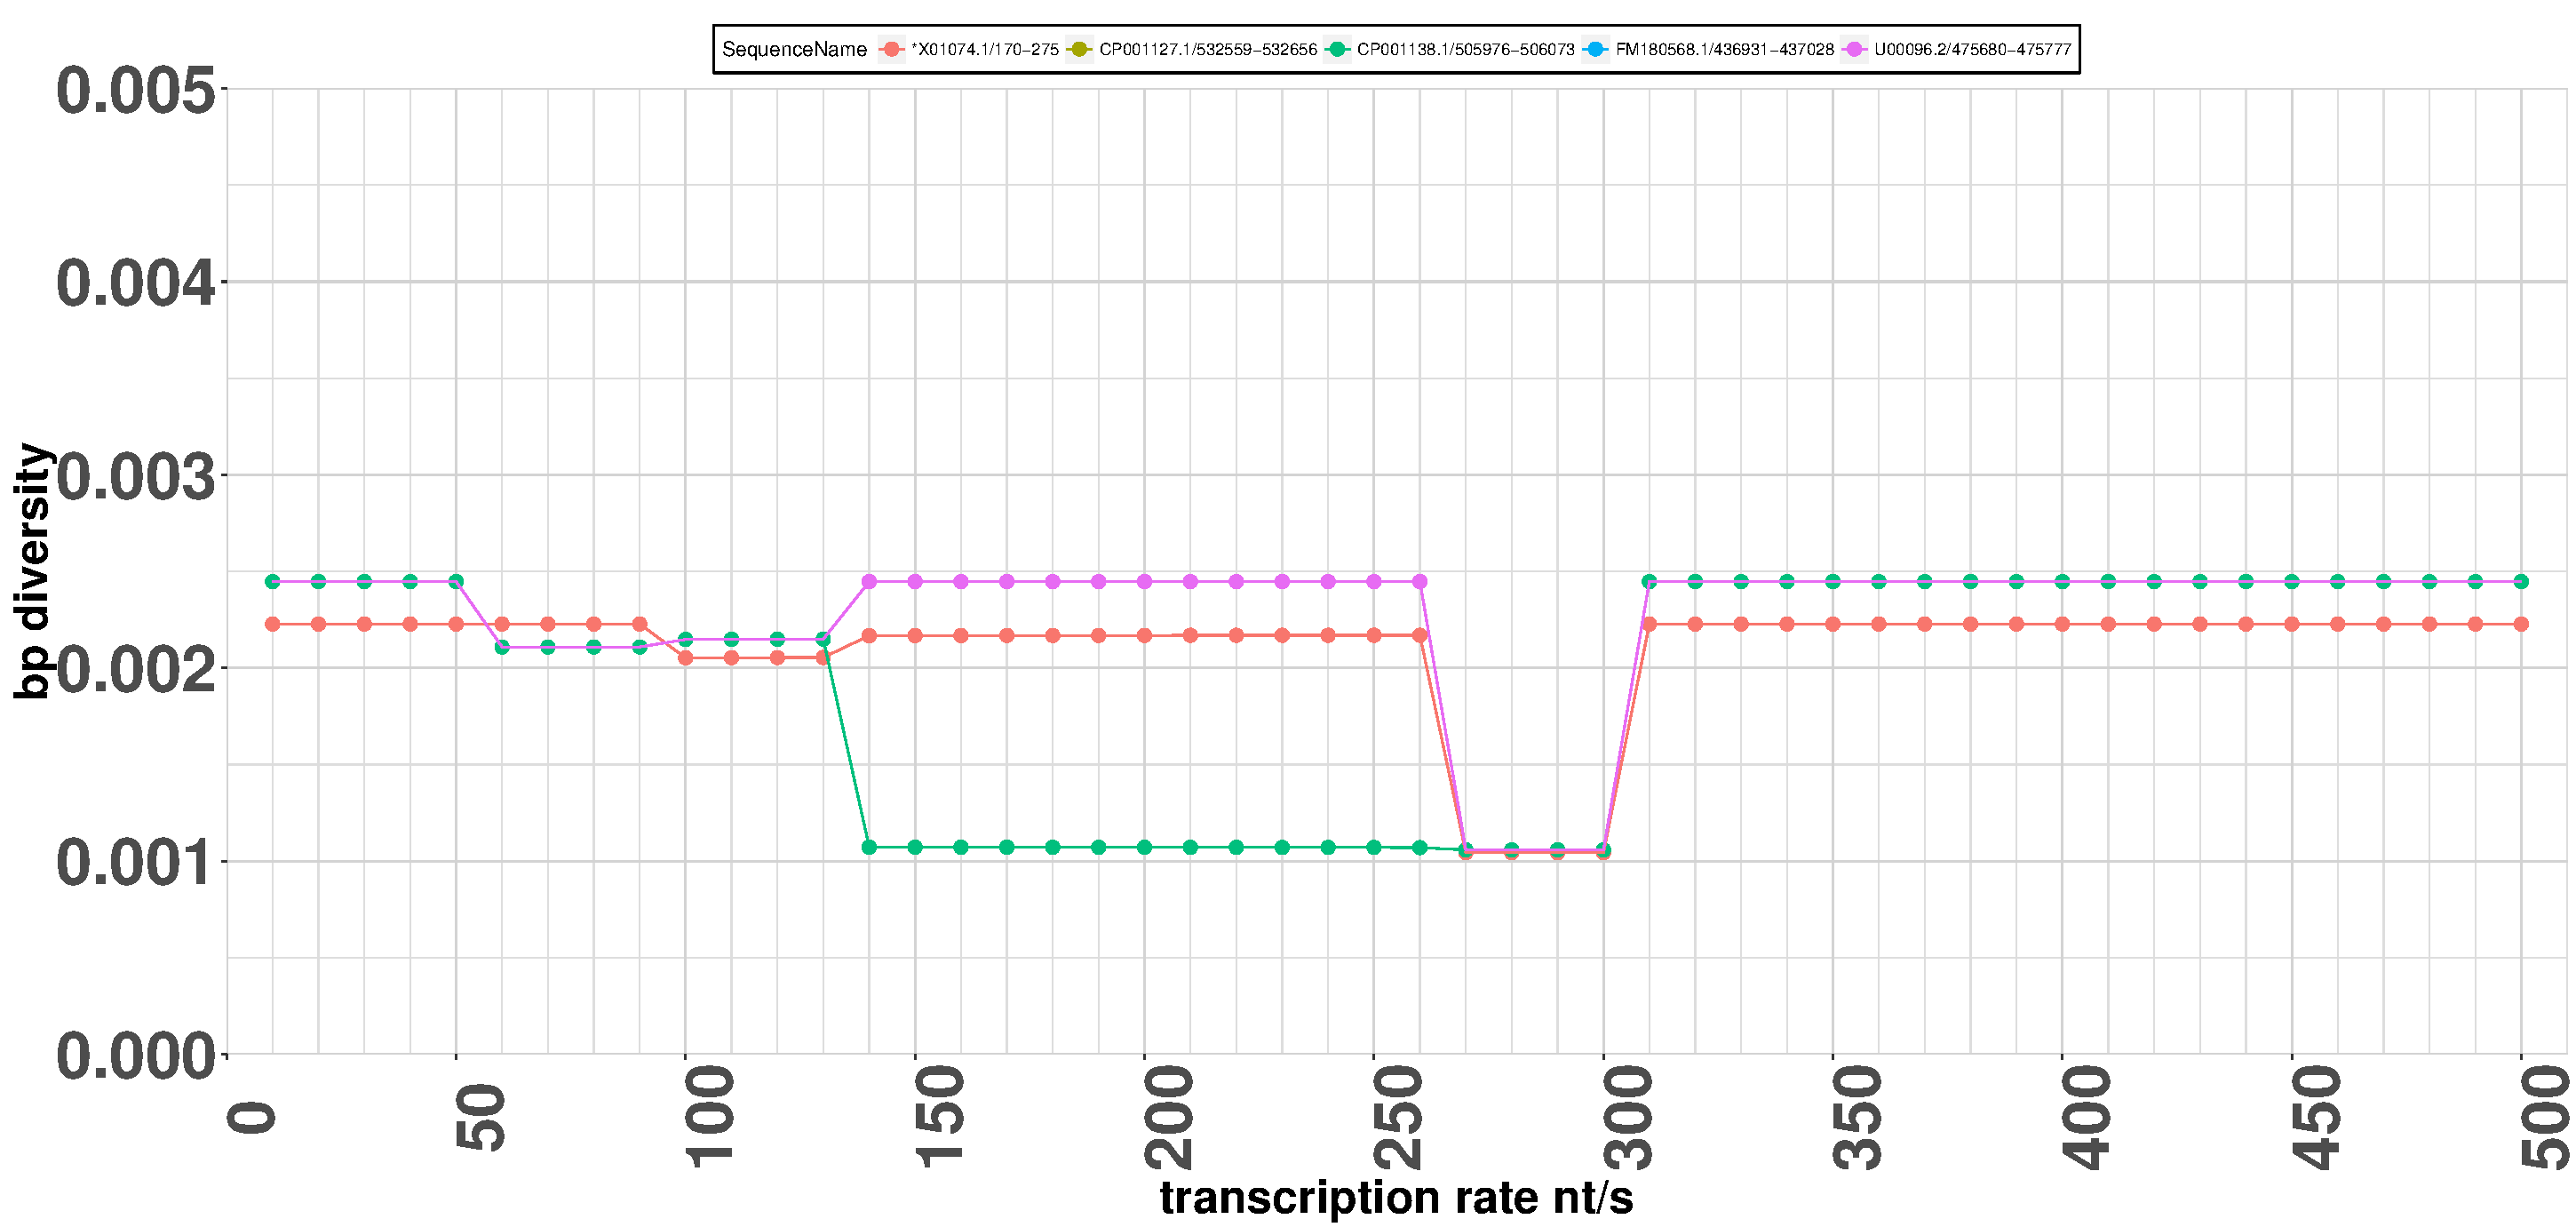
\includegraphics[width=1.0\textwidth]{./pictures/Discussion_results/SRP/SRPseqDecrease250_300nts.pdf}\\

(b) \\
\begin{tabular}{l|l|l|l}
sequence & trap at 260 nt/s  & trap at 300 nt/s & trap at 310 nt/s\\
\hline
X01074.1.170-275			&	yes &	no	&	yes \\
U00096.2.475680-475777		&	yes	&	no	&	yes	\\
FM180568.1.436931-437028	&	yes	&	no	&	yes	\\
CP001138.1.505976-506073	&	yes	&	no	&	yes	\\
CP001127.1.532559-532656 	&	no	&	no	&	yes	\\
CP000058.1.2086711-2086808	&	yes	&	yes	&	yes	\\
\end{tabular}
\\

(c) \\
\begin{tabular}{c|c}
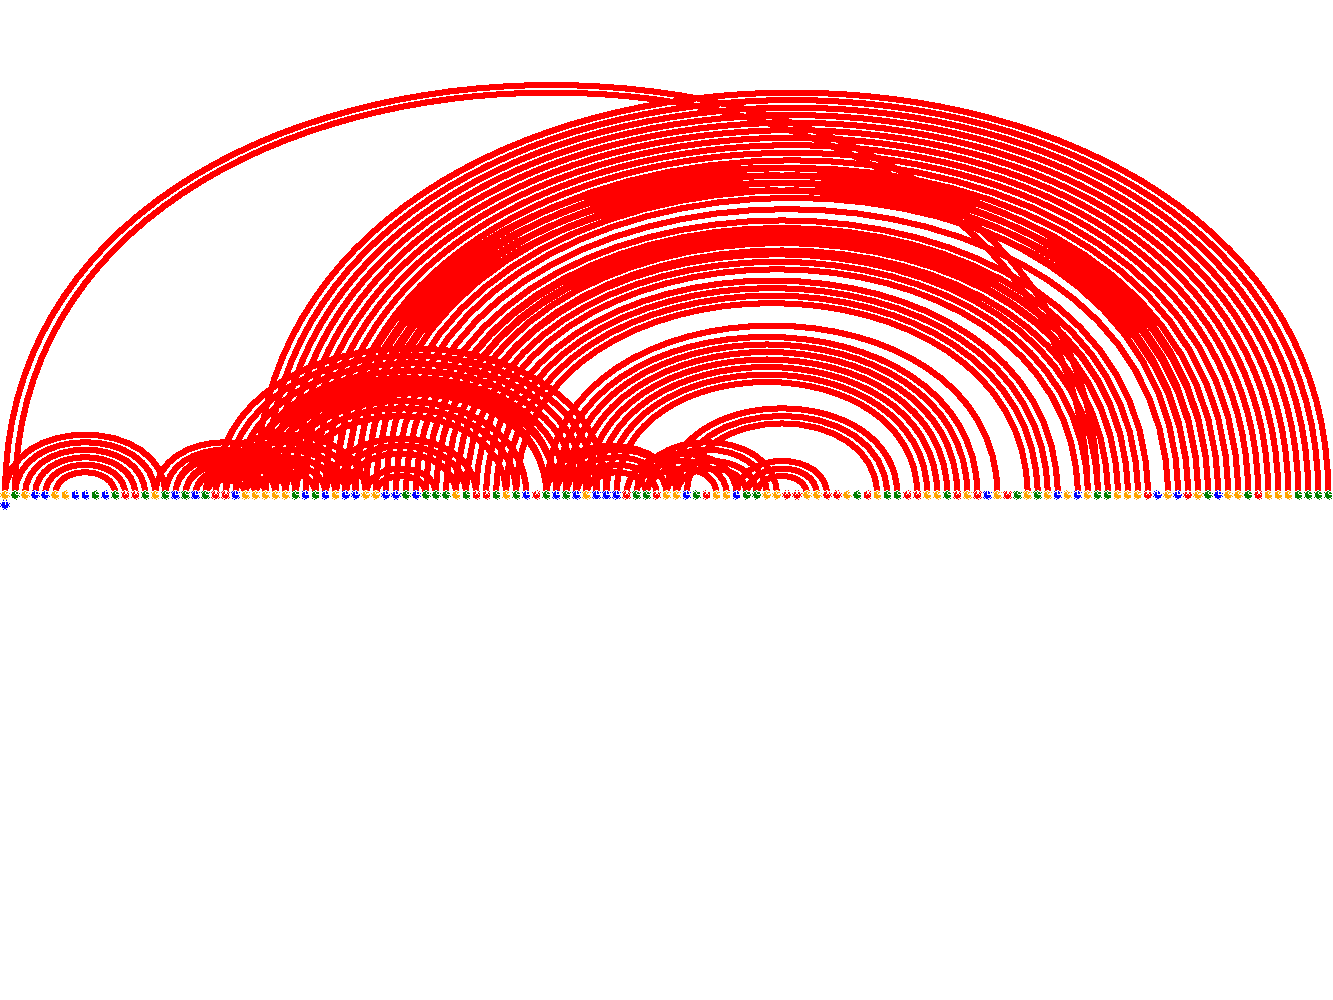
\includegraphics[width=0.5\textwidth]{./pictures/Discussion_results/SRP/X01074_1_170-275_300nts.pdf}&
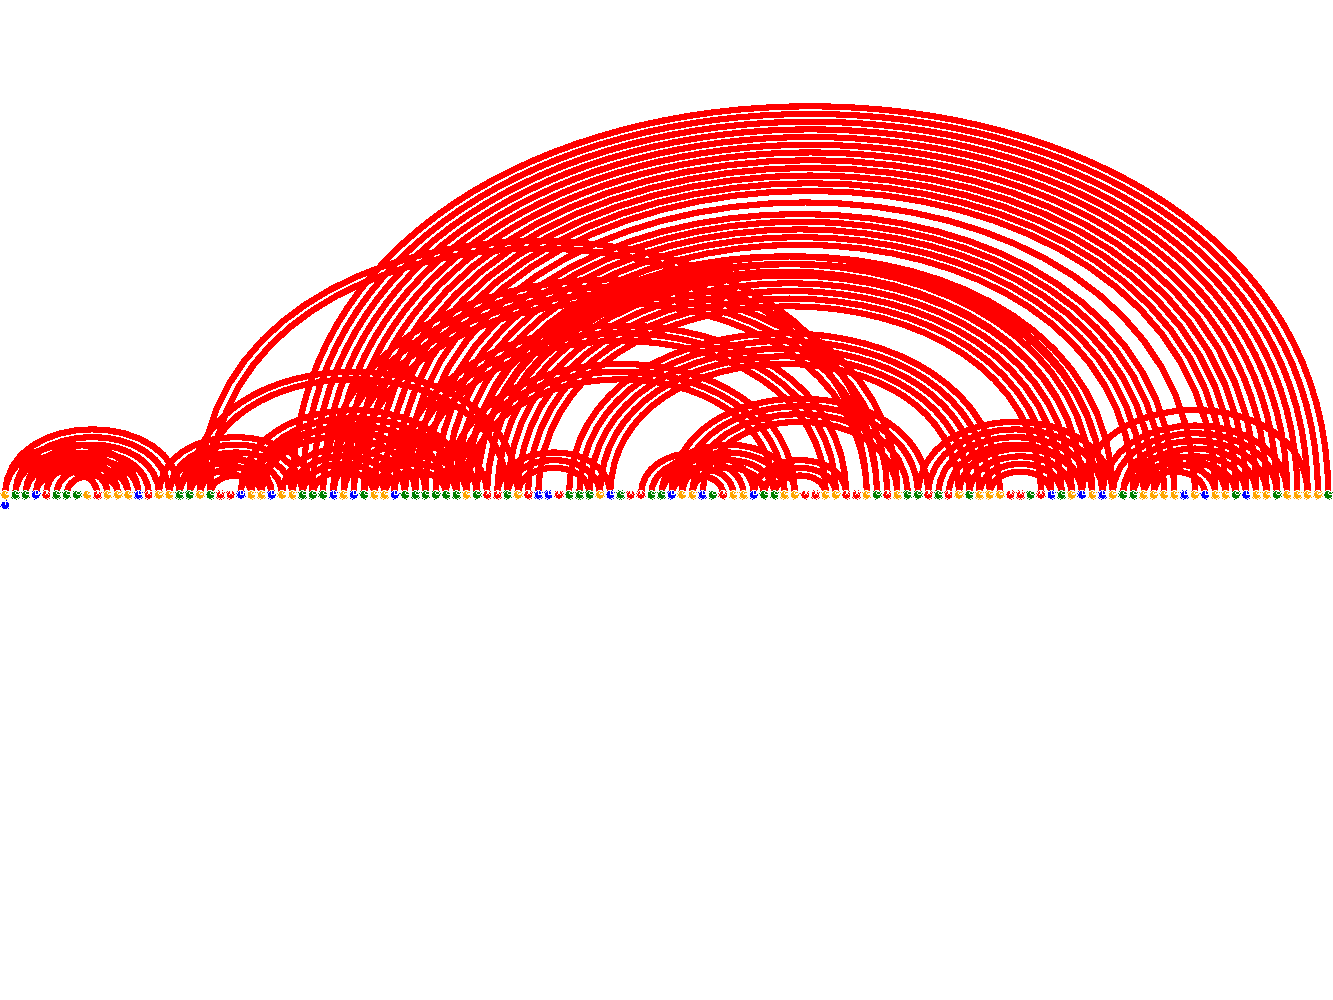
\includegraphics[width=0.5\textwidth]{./pictures/Discussion_results/SRP/X01074_1_170-275_360nts.pdf}\\
\end{tabular}

\end{tabular}

\caption{{\bf Analysis of five interesting \texttt{SRP sequences} }. 
(a) Base-pair diversity for five \texttt{SRP} RNA sequences. Noticeable diversity drop at transcription rates of 270 to 300 nt/s.
(b) Analysis of their folding patterns. All five sequences are folding directly into the MFE structure at this transcription rates. Outside of this transcription rate area, these sequences are folding into a local energy minimum. Sequence \texttt{CP000058.1.2086711-2086808} represents a negative control.
(c) Left: every formed base-pair of the trajectory inside the area. Right: every formed base-pair of the trajectory outside the area}
\label{fig:SRPDecrease250_300}
\end{figure}
\FloatBarrier




\begin{figure}
\begin{tabular}{l}
(a) \\
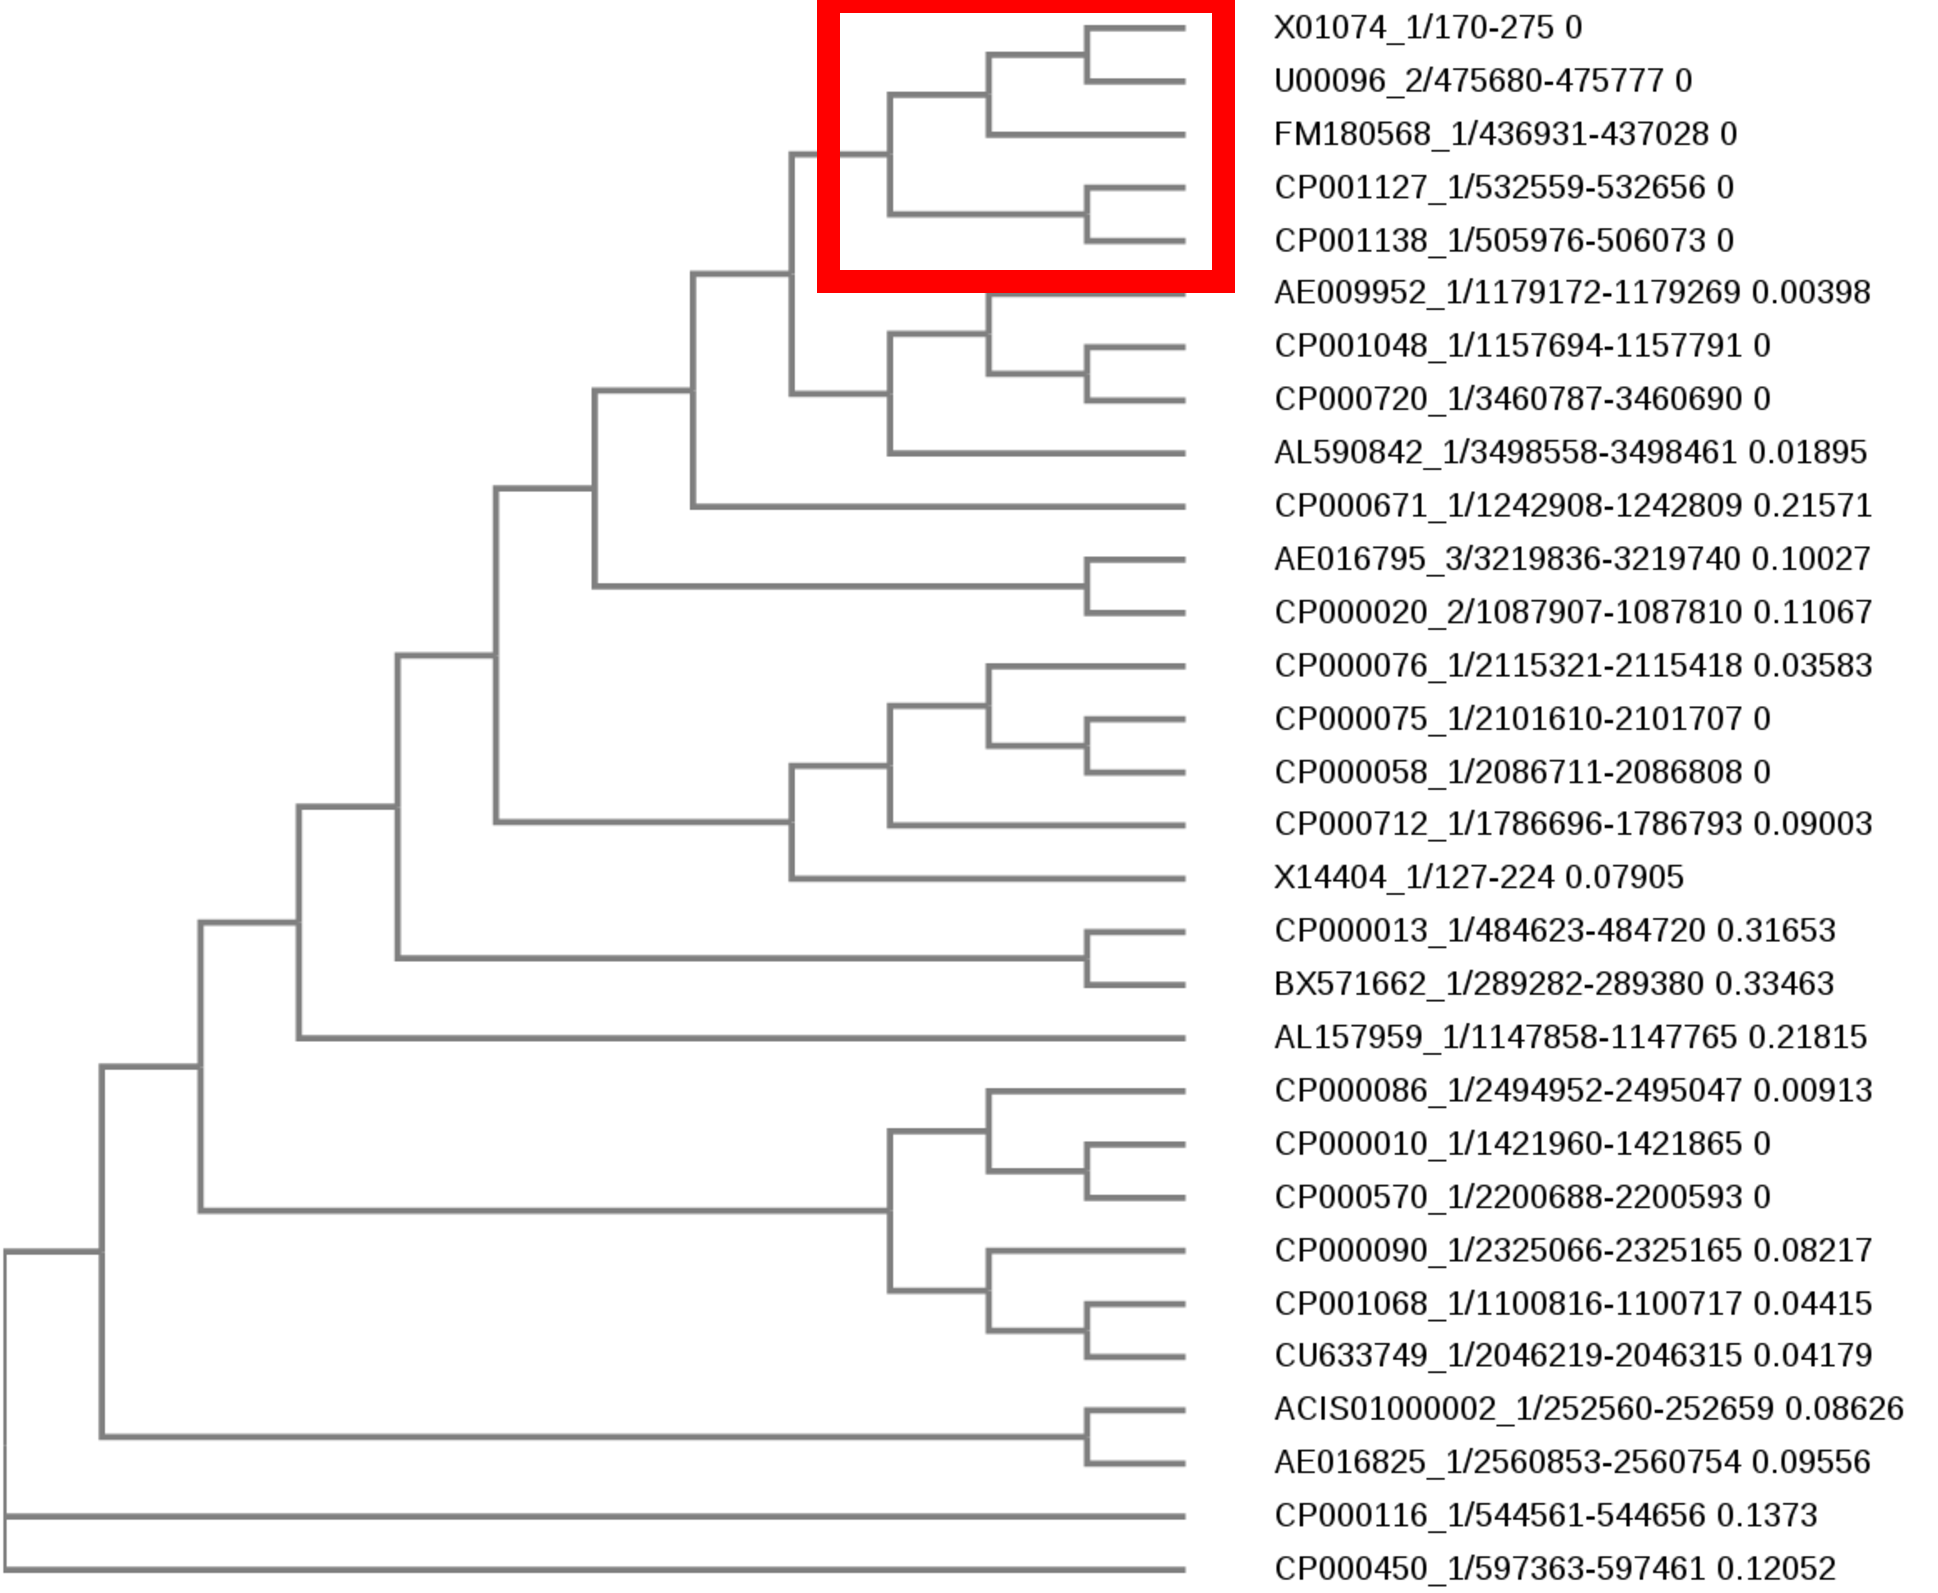
\includegraphics[width=0.7\textwidth]{./pictures/Discussion_results/SRP/srp_pylotree.pdf}\\
(b) \\
\includegraphics[width=0.7\textwidth]{./pictures/Discussion_results/SRP/MSA_SRP_5seq.png}\\
\end{tabular}

\caption{{\bf phylogenetic tree and MSA for \texttt{SRP} family} 
(a) \texttt{SRP} phylogenetic tree, created by \texttt{ClustalW2 to Phylogeny}. All five sequences are in one subgroup.
(b) Multiple sequence alignment shows that these five sequences have a similarity of nearly 100 \%.
}
\label{fig:SRP_PhyloTree}
\end{figure}
\FloatBarrier





%Last conclusion

\section{summary and outlook}

%Note: \texttt{Kinwalker} algorithm is assuming that the transcription rate is constant, which is not true for in vivo%!!!\citep{transcriptionPausing},%!!!\cite{trspeed} and also no effort is made to regard trans interactions( e.g. proteins or other RNAs).



I calculated and studied the co-transcriptional folding trajectories for three well studied RNA families by using the program \texttt{Kinwalker}, to detect evidences for co-transcriptional folding conservation. Overall I calculated folding trajectories with 200 different parameter combinations and scored and plotted the results. 
In conclusion, I did not found any evidence for co-transcriptional folding conservation for the threes studied RNA families. Apart from that, I obtained evidence for sequences conservation within the \texttt{Enterobacteriaceae} family for \texttt{SRP} RNA sequences.
Furthermore, I found out that transcription rates have a high influence on the folding of the \texttt{SRP} reference sequence, and I located a parameter set which is optimal for \texttt{Kinwalker} co-transcriptional folding prediction for this one sequence.


For further studies, the parameter space, especially transcription rate, should be further investigated (extending rate beyond 500 nt/s and with smaller intervals). 
Further improvement of the scores could also lead to better results. Especially improving the ensemble distance score would be desired by adding constraint folding to be certain that a specific intermediate structure is part of the folding trajectory.

Furthermore, the general scoring of base-pairs should be improved. A base-pair that could be formed due to compatible bases -but has not- should get a different scoring than a base-pair that could never form this base-pair due to incompatible bases.
  
%I regarded the reference structure more important than
%necessary. More meaningful would be the comparison of every folding
%trajectory with a structure [S]. Structure [S] is unknown to me but should
%be the lowest common denominator (structure) of the folding trajectory of
%an alignment. To calculate such structure, following approach could be
%used: Given is a reference structure pool R. Sum of all ensemble distances
%(for all alignment sequences) to every element of R results with the
%average ensemble distance of one alignment to one R. R with the minimal
%distance is the theoretically [S] structure for this alignment.





\chapter{Appendix}

\begin{sidewaystable}
\centering
%\begin{table}
%\begin{tabular}{p{5cm}|p{5cm}|p{5cm}}
\begin{tabular}{l|l|l|l}
RF00169 (\texttt{SRP}) & RF00513 (trpL) & RF00010 (RNaseP)\\
\hline \\[1pt]

\includegraphics[width=0.3\textwidth]{./pictures/SRPSequences.png} & 
\includegraphics[width=0.3\textwidth]{./pictures/TRPSequences.png} & 
\includegraphics[width=0.3\textwidth]{./pictures/RNAsePSequences.png}\\
\end{tabular}
\caption{{\bf RNA sequence composition of Rfam families.}
Identifier is the \texttt{GenBank accession number}. Plus strand is taken if the start base-pair position is lower than the end base-pair position and vica versa.}
\label{table:alignment composition}
%\end{table}
\end{sidewaystable}

\begin{table}
\tiny
\begin{tabular}{l|l}
accession number &	species name \\
\hline
X01074.1/170-275		&Escherichia coli 4.5S\\
AE016795.3/3219836-3219740& 	Vibrio vulnificus CMCP6 chromosome I, complete sequence\\
CP000671.1/1242908-1242809 &	Haemophilus influenzae PittEE, complete genome\\
ACIS01000002.1/252560-252659& 	Pseudogulbenkiania ferrooxidans 2002 ctg6, whole genome shotgun sequence\\
CP000076.1/2115321-2115418 	&Pseudomonas protegens Pf-5, complete genome\\
CP000712.1/1786696-1786793 	&Pseudomonas putida F1, complete genome\\
CP000013.1/484623-484720 	&Borrelia garinii PBi, complete genome\\
CP001127.1/532559-532656 	&Salmonella enterica subsp. enterica serovar Schwarzengrund str. CVM19633, complete genome\\
CP000086.1/2494952-2495047 	&Burkholderia thailandensis E264 chromosome I, complete sequence\\
AE009952.1/1179172-1179269 	&Yersinia pestis KIM10+, complete genome\\
AL157959.1/1147858-1147765 	&Neisseria meningitidis serogroup A strain Z2491 complete genome\\
CP000090.1/2325066-2325165 	&Ralstonia eutropha JMP134 chromosome 1, complete sequence\\
CP000116.1/544561-544656 	&Thiobacillus denitrificans ATCC 25259, complete genome\\
CP001048.1/1157694-1157791 	&Yersinia pseudotuberculosis PB1/+, complete genome\\
CP001068.1/1100816-1100717 	&Ralstonia pickettii 12J chromosome 1, complete sequence\\
CP001138.1/505976-506073 	&Salmonella enterica subsp. enterica serovar Agona str. SL483, complete genome\\
CU633749.1/2046219-2046315 	&Cupriavidus taiwanensis str. LMG19424 chromosome 1, complete genome\\
U00096.2/475680-475777 		&Escherichia coli str. K-12 substr. MG1655, complete genome\\
CP000075.1/2101610-2101707 	&Pseudomonas syringae pv. syringae B728a, complete genome\\
FM180568.1/436931-437028 	&Escherichia coli 0127:H6 E2348/69 complete genome, strain E2348/69\\
CP000020.2/1087907-1087810 	&Vibrio fischeri ES114 chromosome I, complete sequence\\
BX571662.1/289282-289380 	&Wolinella succinogenes, complete genome; segment 6/7\\
CP000720.1/3460787-3460690 	&Yersinia pseudotuberculosis IP 31758, complete genome\\
CP000450.1/597363-597461 	&Nitrosomonas eutropha C91, complete genome\\
AL590842.1/3498558-3498461 	&Yersinia pestis CO92 complete genome\\
AE016825.1/2560853-2560754 	&Chromobacterium violaceum ATCC 12472, complete genome\\
CP000010.1/1421960-1421865 	&Burkholderia mallei ATCC 23344 chromosome 1, complete sequence\\
CP000570.1/2200688-2200593 	&Burkholderia pseudomallei 668 chromosome I, complete sequence\\
CP000058.1/2086711-2086808 	&Pseudomonas syringae pv. phaseolicola 1448A, complete genome\\
X14404.1/127-224 		&Pseudomonas aeruginosa 4.5S RNA homologue\\
\end{tabular}
\caption{{\bf translation from accession-number to species name for \texttt{SRP} family }}
\label{table:SRPAcessionToSpeciesName}
\end{table}

\begin{figure}
\includegraphics[width=0.8\textwidth]{./Appendix/SRP_SpeciesTree}
\caption{{\bf species tree for \texttt{SRP} family}}
\label{fig:SRPSpeciesTree}
\end{figure}



%********************************************************************
% Bibliography
%*******************************************************
% work-around to have small caps also here in the headline
\manualmark
\markboth{\spacedlowsmallcaps{\bibname}}{\spacedlowsmallcaps{\bibname}} % work-around to have small caps also
%\phantomsection 
\refstepcounter{dummy}
\addtocontents{toc}{\protect\vspace{\beforebibskip}} % to have the bib a bit from the rest in the toc
\addcontentsline{toc}{chapter}{\tocEntry{\bibname}}
\bibliographystyle{plainnat}
\label{app:bibliography} 
\bibliography{Bibliography}
\end{document}


